% Options for packages loaded elsewhere
% Options for packages loaded elsewhere
\PassOptionsToPackage{unicode}{hyperref}
\PassOptionsToPackage{hyphens}{url}
\PassOptionsToPackage{dvipsnames,svgnames,x11names}{xcolor}
%
\documentclass[
  12pt,
  oneside]{book}
\usepackage{xcolor}
\usepackage[top=30mm,bottom=30mm,left=25mm,right=20mm,headheight=15mm,footskip=33pt]{geometry}
\usepackage{amsmath,amssymb}
\setcounter{secnumdepth}{5}
\usepackage{iftex}
\ifPDFTeX
  \usepackage[T1]{fontenc}
  \usepackage[utf8]{inputenc}
  \usepackage{textcomp} % provide euro and other symbols
\else % if luatex or xetex
  \usepackage{unicode-math} % this also loads fontspec
  \defaultfontfeatures{Scale=MatchLowercase}
  \defaultfontfeatures[\rmfamily]{Ligatures=TeX,Scale=1}
\fi
\usepackage{lmodern}
\ifPDFTeX\else
  % xetex/luatex font selection
\fi
% Use upquote if available, for straight quotes in verbatim environments
\IfFileExists{upquote.sty}{\usepackage{upquote}}{}
\IfFileExists{microtype.sty}{% use microtype if available
  \usepackage[]{microtype}
  \UseMicrotypeSet[protrusion]{basicmath} % disable protrusion for tt fonts
}{}
\usepackage{setspace}
\makeatletter
\@ifundefined{KOMAClassName}{% if non-KOMA class
  \IfFileExists{parskip.sty}{%
    \usepackage{parskip}
  }{% else
    \setlength{\parindent}{0pt}
    \setlength{\parskip}{6pt plus 2pt minus 1pt}}
}{% if KOMA class
  \KOMAoptions{parskip=half}}
\makeatother
% Make \paragraph and \subparagraph free-standing
\makeatletter
\ifx\paragraph\undefined\else
  \let\oldparagraph\paragraph
  \renewcommand{\paragraph}{
    \@ifstar
      \xxxParagraphStar
      \xxxParagraphNoStar
  }
  \newcommand{\xxxParagraphStar}[1]{\oldparagraph*{#1}\mbox{}}
  \newcommand{\xxxParagraphNoStar}[1]{\oldparagraph{#1}\mbox{}}
\fi
\ifx\subparagraph\undefined\else
  \let\oldsubparagraph\subparagraph
  \renewcommand{\subparagraph}{
    \@ifstar
      \xxxSubParagraphStar
      \xxxSubParagraphNoStar
  }
  \newcommand{\xxxSubParagraphStar}[1]{\oldsubparagraph*{#1}\mbox{}}
  \newcommand{\xxxSubParagraphNoStar}[1]{\oldsubparagraph{#1}\mbox{}}
\fi
\makeatother


\usepackage{longtable,booktabs,array}
\newcounter{none} % for unnumbered tables
\usepackage{calc} % for calculating minipage widths
% Correct order of tables after \paragraph or \subparagraph
\usepackage{etoolbox}
\makeatletter
\patchcmd\longtable{\par}{\if@noskipsec\mbox{}\fi\par}{}{}
\makeatother
% Allow footnotes in longtable head/foot
\IfFileExists{footnotehyper.sty}{\usepackage{footnotehyper}}{\usepackage{footnote}}
\makesavenoteenv{longtable}
\usepackage{graphicx}
\makeatletter
\newsavebox\pandoc@box
\newcommand*\pandocbounded[1]{% scales image to fit in text height/width
  \sbox\pandoc@box{#1}%
  \Gscale@div\@tempa{\textheight}{\dimexpr\ht\pandoc@box+\dp\pandoc@box\relax}%
  \Gscale@div\@tempb{\linewidth}{\wd\pandoc@box}%
  \ifdim\@tempb\p@<\@tempa\p@\let\@tempa\@tempb\fi% select the smaller of both
  \ifdim\@tempa\p@<\p@\scalebox{\@tempa}{\usebox\pandoc@box}%
  \else\usebox{\pandoc@box}%
  \fi%
}
% Set default figure placement to htbp
\def\fps@figure{htbp}
\makeatother





\setlength{\emergencystretch}{3em} % prevent overfull lines

\providecommand{\tightlist}{%
  \setlength{\itemsep}{0pt}\setlength{\parskip}{0pt}}



 


\usepackage{Archivo}
%\usepackage[sc]{mathpazo}

\usepackage[T1]{fontenc}
\usepackage{xcolor}
\usepackage[pages=some]{background}
\usepackage{setspace}
\usepackage[table]{xcolor}
\usepackage{tabularx}
\usepackage[Bjornstrup]{fncychap}
\usepackage{multirow}

% Colors Techtraplastice
\definecolor{Naranja}{HTML}{F69223}
\definecolor{Celeste}{HTML}{3299CC}
\definecolor{Verde}{HTML}{98C601}
\definecolor{Neutro}{HTML}{5E6F75}
\definecolor{Neutro_claro}{HTML}{F1F1F1}

\definecolor{Verde_osc}{RGB}{47,93,80}


% Headers
\usepackage{fancyhdr}
\pagestyle{fancy}          

\fancyhead{}
\fancyfoot{}

\fancyhead[L]{
\includegraphics[height=10mm]{assets/images/logo-TTPCE.png}}
\fancyhead[C]{ }
\fancyhead[R]{\thepage}

\fancyfoot[L]{
\includegraphics[height=8mm]{assets/images/footer-00.png}}
\fancyfoot[C]{}
\fancyfoot[R]{
\includegraphics[height=8mm]{assets/images/EU.png}}



\renewcommand{\headrulewidth}{1pt}
\renewcommand{\headruleskip}{1mm}



\usepackage{pdfpages}
\usepackage{wrapfig}
\usepackage{pgfgantt}
\usepackage{academicons}

\usepackage{worldflags}

% Command
\newcommand{\techtra}{\emph{TechTraPlastiCE }}

\usepackage{tabu}

% \usepackage{sectsty}
% \sectionfont{\scshape}
\usepackage{booktabs}
\usepackage{longtable}
\usepackage{array}
\usepackage{multirow}
\usepackage{wrapfig}
\usepackage{float}
\usepackage{colortbl}
\usepackage{pdflscape}
\usepackage{tabularx}
\usepackage{xltabular}
\usepackage{threeparttable}
\usepackage{threeparttablex}
\usepackage[normalem]{ulem}
\usepackage{makecell}
\usepackage{xcolor}
\makeatletter
\@ifpackageloaded{caption}{}{\usepackage{caption}}
\AtBeginDocument{%
\ifdefined\contentsname
  \renewcommand*\contentsname{Table of contents}
\else
  \newcommand\contentsname{Table of contents}
\fi
\ifdefined\listfigurename
  \renewcommand*\listfigurename{List of Figures}
\else
  \newcommand\listfigurename{List of Figures}
\fi
\ifdefined\listtablename
  \renewcommand*\listtablename{List of Tables}
\else
  \newcommand\listtablename{List of Tables}
\fi
\ifdefined\figurename
  \renewcommand*\figurename{Figure}
\else
  \newcommand\figurename{Figure}
\fi
\ifdefined\tablename
  \renewcommand*\tablename{Table}
\else
  \newcommand\tablename{Table}
\fi
}
\@ifpackageloaded{float}{}{\usepackage{float}}
\floatstyle{ruled}
\@ifundefined{c@chapter}{\newfloat{codelisting}{h}{lop}}{\newfloat{codelisting}{h}{lop}[chapter]}
\floatname{codelisting}{Listing}
\newcommand*\listoflistings{\listof{codelisting}{List of Listings}}
\makeatother
\makeatletter
\usepackage{pdflscape}
\makeatother
\makeatletter
\makeatother
\makeatletter
\@ifpackageloaded{caption}{}{\usepackage{caption}}
\@ifpackageloaded{subcaption}{}{\usepackage{subcaption}}
\makeatother
\usepackage{bookmark}
\IfFileExists{xurl.sty}{\usepackage{xurl}}{} % add URL line breaks if available
\urlstyle{same}
% fallback for those not using the hyperref driver hyperxmp:
\makeatletter
\@ifundefined{xmpquote}{\newcommand{\xmpquote}[1]{#1}}{}
\makeatother
\hypersetup{
  pdftitle={D2.1 Repository with Proposed Solutions / Services},
  pdfauthor={Prof.~Paula Ferreira (UA), Prof.~Idalina José Gonçalves (UA), Prof.~Cláudia Nunes (UA).; Prof.~Yamila Victoria Vazquez (UNS), Prof.~Yanela N. Alonso (UNS), Prof.~Luciana A. Castillo, (UNS), Econ. Yesica Soledad Dilernia (UNS), ID. Teresa Dutari (UNS).},
  colorlinks=true,
  linkcolor={Celeste},
  filecolor={Maroon},
  citecolor={Blue},
  urlcolor={Naranja},
  pdfcreator={LaTeX via pandoc}}


\title{D2.1 Repository with Proposed Solutions / Services}
\author{Prof.~Paula Ferreira (UA), Prof.~Idalina José Gonçalves (UA),
Prof.~Cláudia Nunes (UA). \and Prof.~Yamila Victoria Vazquez (UNS),
Prof.~Yanela N. Alonso (UNS), Prof.~Luciana A. Castillo, (UNS), Econ.
Yesica Soledad Dilernia (UNS), ID. Teresa Dutari (UNS).}
\date{November 25, 2026}
\begin{document}
  \begin{frontmatter}
  \begin{titlepage}
  % Inspiration: https://nmfs-opensci.github.io/quarto_titlepages_v1/02-titlepages.html
  % This is a combination of Pandoc templating and LaTeX
  % Pandoc templating https://pandoc.org/MANUAL.html#templates
  % See the README for help



  \backgroundsetup{
    scale=1.0,
    angle=0,
    opacity=0.90,
    contents={
      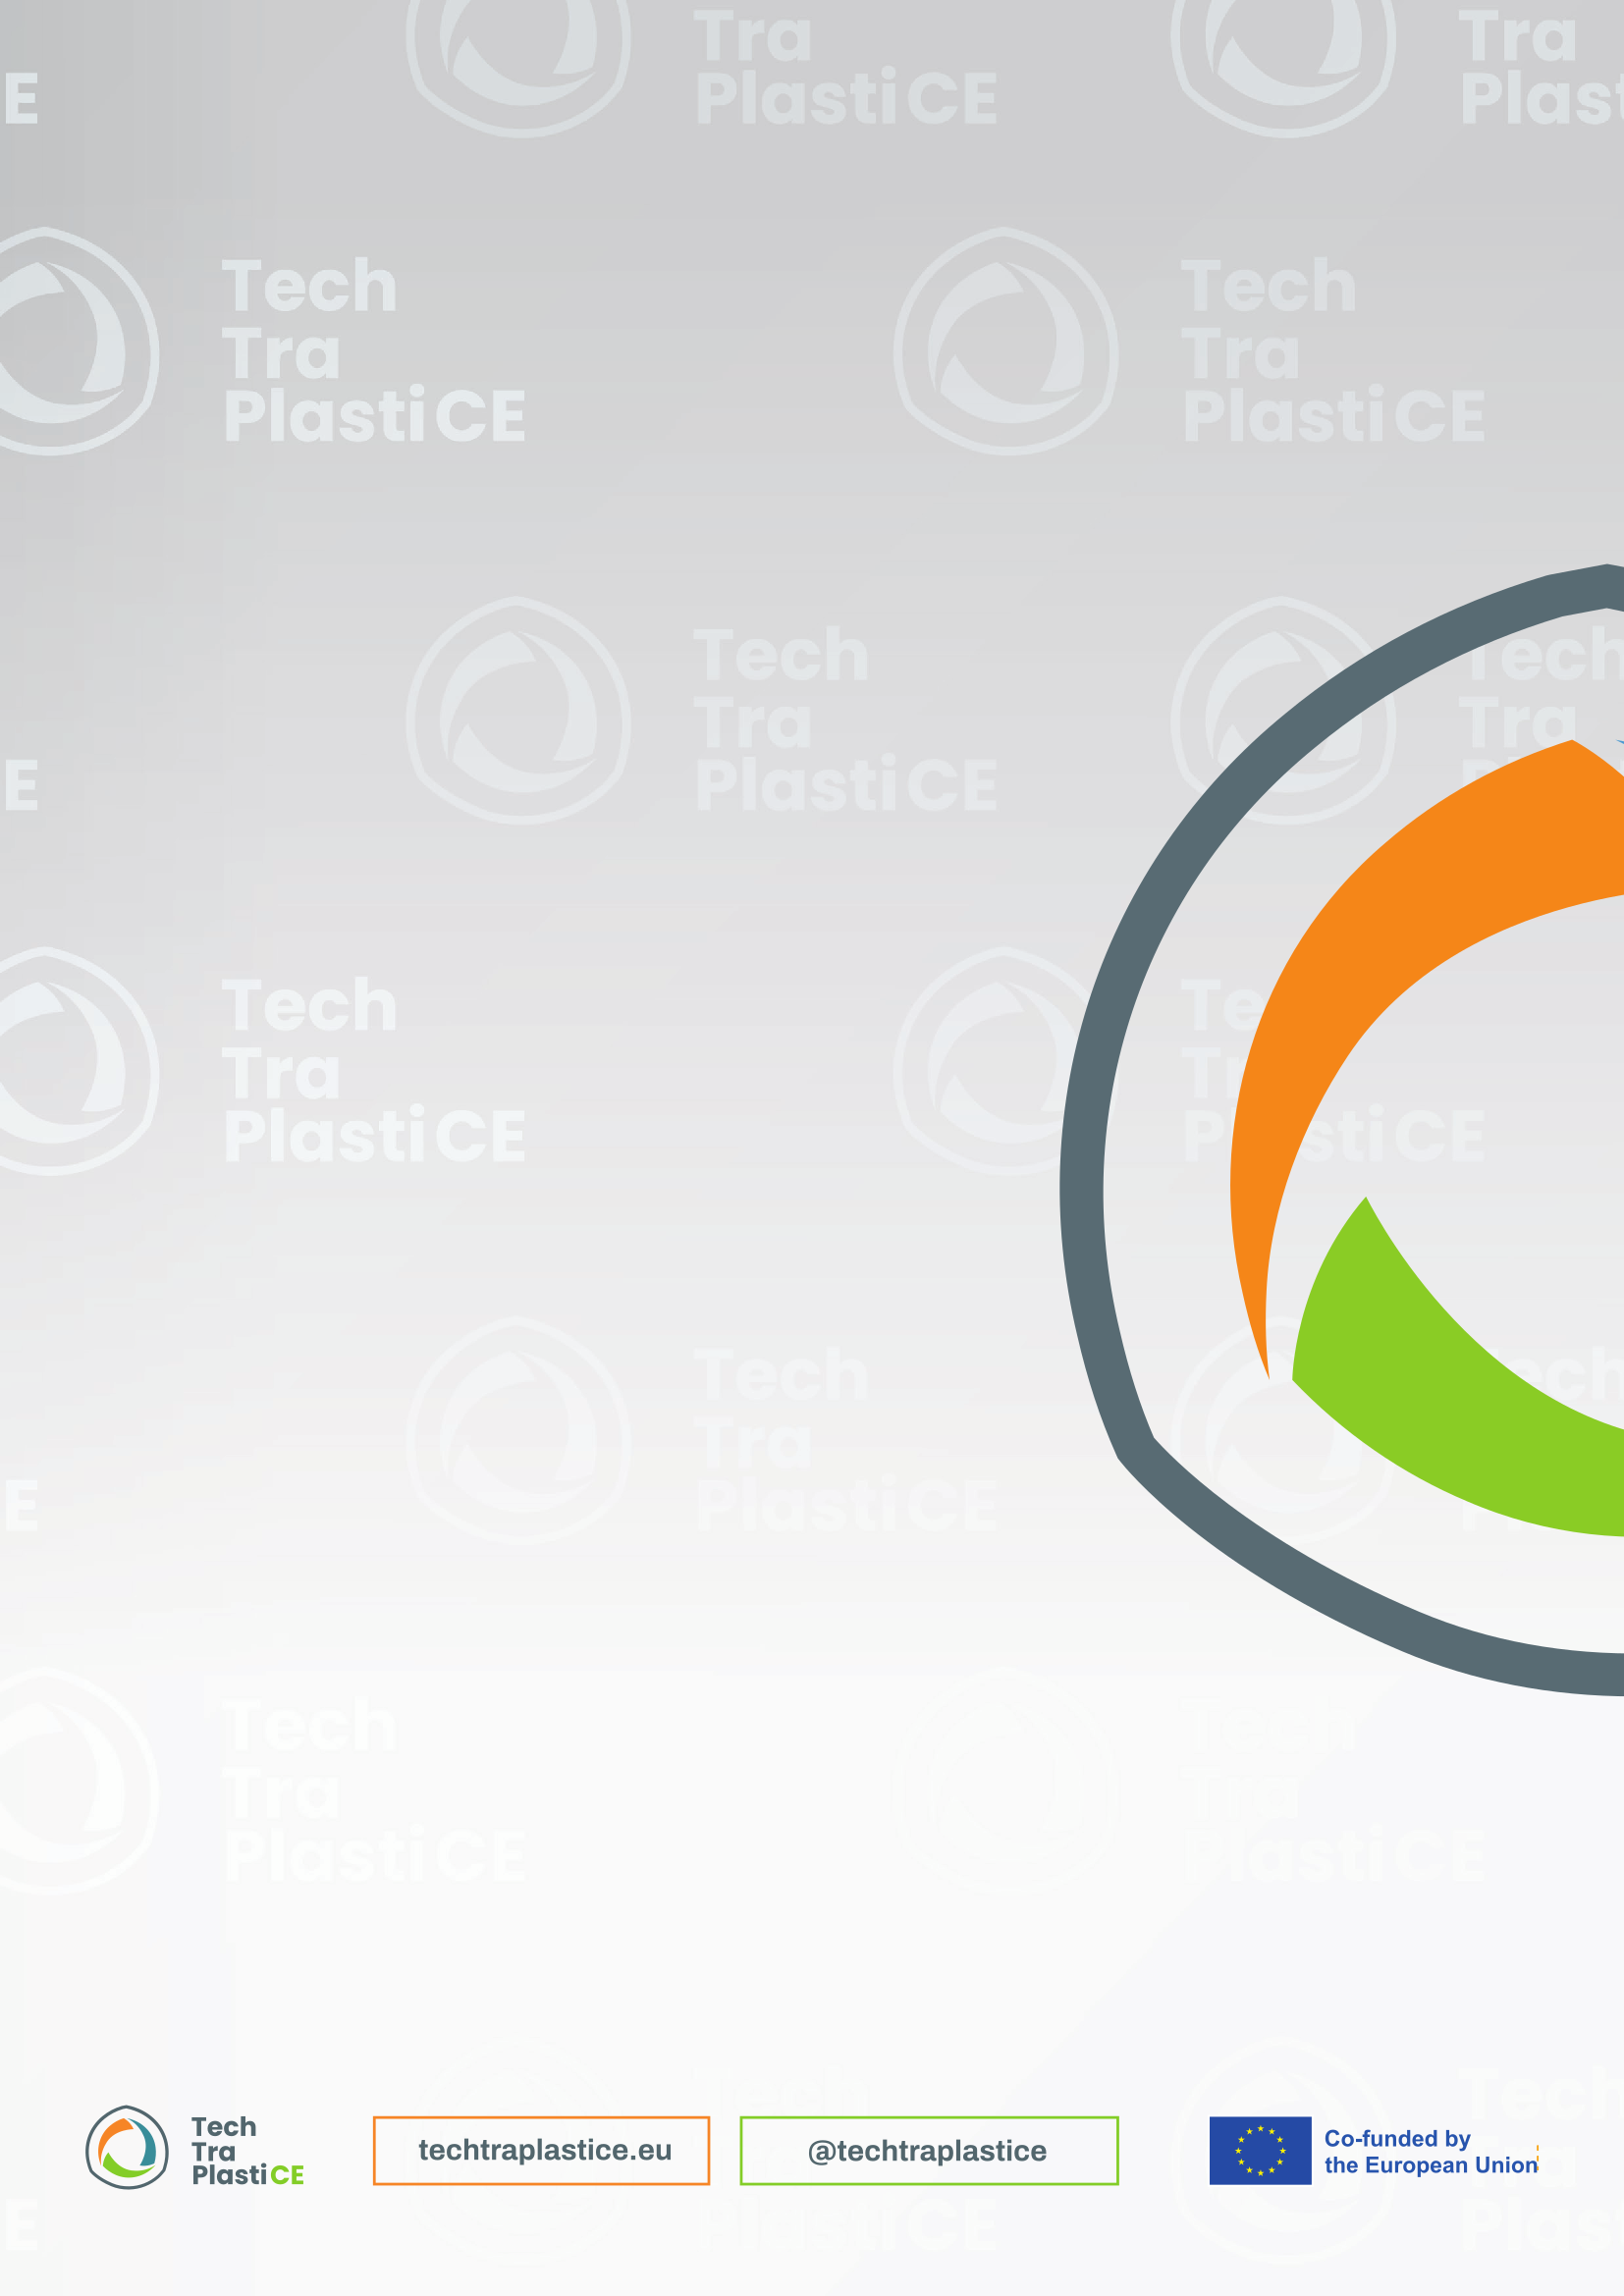
\includegraphics{assets/Portada.png}}
      }

  \BgThispage


  \begin{minipage}[b][0.78\textheight][s]{0.65\textwidth}

    \raggedright
    % Title and subtitle
    
    \vfill

    \begin{spacing}{2.2}
      {\color{Naranja}\Huge\bfseries{D2.1 Repository with Proposed
  Solutions / Services}} \\[1\baselineskip] 
    \end{spacing}
    
    \begin{spacing}{1.2}
    {\color{Neutro} \Large\textit{WP2: Development of a networked
  portfolio}}\\[1\baselineskip]
    
    {\Large \color{Neutro} 
    Strengthening University Tech Transfer Capabilities to Support Circular Economy 
    Value Chains for Plastics in Latin America -
    \textsc{\centering\bfseries TechTraPlastiCE} }\\[2\baselineskip]

    
    \end{spacing}

    {\color{Neutro} \Large\textit{November 25, 2026}}
    
    \vfill
  \end{minipage}		

  \vfill

  {\scriptsize
    \color{Neutro}
    This project has been funded with the support of Erasmus +.  
    The contents are the responsibility of the author(s). 
    The Commission cannot be held responsible for any use which may be made of the information contained therein. 
    Project No. 101179564 
    }


  \newpage



  \thispagestyle{plain}
  \begin{tabu} to \linewidth {X[1.3,l]  | X[1,l] X[1,l]}
    \toprule
    \multirow{5}{*}{ 
\includegraphics[height=20mm]{assets/images/logo-TTPCE.png}} &  \textbf{Work Package} : & WP2  \\ \cmidrule{2-3}
      & \textbf{Project Number} : & 101179564  \\ \cmidrule{2-3}
      &  \textbf{Type of document}:  & Deliverable   \\ \cmidrule{2-3}
      & \textbf{Due Delivery Date}:    & April
  30/2026     \\ \cmidrule{2-3}
      & \textbf{Actual Delivery Date}:    & November 25, 2026       \\ 
    \bottomrule
  \end{tabu}

  \vfill


  \begin{tabu} to \linewidth {X[1,l]  | X[3.5,l]}
    \toprule
    \textbf{Title} : & D2.1 Repository with Proposed Solutions /
  Services  \\ \cmidrule{2-2}
    \textbf{Work Package} : & WP2: Development of a networked
  portfolio  \\ \cmidrule{2-2}
    \textbf{Description} : & This repository will consist of digital
  documents/pieces grouping in a visual manner the collective portfolio,
  the providers, and the main assets of partner institutions; to openly
  sharing with different targets/industries.  \\ \cmidrule{2-2}
    \textbf{Responsible} : & Universidad Nacional del Sur \&
  Universidade de Aveiro  \\ \cmidrule{2-2}
    \textbf{Author(s)} : &  
     
          Prof.~Paula Ferreira (UA), Prof.~Idalina José Gonçalves (UA),
          Prof.~Cláudia Nunes (UA).
          
          Prof.~Yamila Victoria Vazquez (UNS), Prof.~Yanela N. Alonso
          (UNS), Prof.~Luciana A. Castillo, (UNS), Econ. Yesica Soledad
          Dilernia (UNS), ID. Teresa Dutari (UNS).
           \\ \cmidrule{2-2}
    \textbf{Project Call} : & ERASMUS-EDU-2024-CBHE (Capacity building in the field of higher education)  \\ \cmidrule{2-2}
    \textbf{Dissemination Level} : & Public\\   
  \bottomrule
  \end{tabu}



  \vfill


  \begin{tabular}{ >{\raggedright\arraybackslash}p{3cm}| p{2cm} p{4cm} p{6cm} }
    \toprule
    \textbf{Version}: & \multicolumn{3}{l}{ 1.2} \\ \midrule
    \textbf{Contributors}  & Versions    & Dates       & Revision Description \\ \midrule
    UA  & 1    & 20/04/2026  & Initial draft of the D.2.1 deliverable  \\ 
    UN  & 1.1    & 28/04/2026  & Reviewed the consolidated document and feedback on presentation of results.  \\ 
    UL  & 1.2   & 04/05/2026  & Final consolidation and integration of all feedback  \\ 
    \bottomrule
\end{tabular}  


    
    
    \vfill
    
    {\scriptsize\centering\color{lightgray} 
    
    Disclaimer
    
    This document is provided <<as is>> with no warranties whatsoever, 
    including any warranty or merchantability, non-infringement, fitness for any particular 
    purpose, or any warranty otherwise arising out of any proposal, specification or sample.  
    
    No license, express or implied, by estoppels or otherwise, to any intellectual 
    property rights are granted herein. 
    The members of the project TechTraPlastiCE do not accept any liability for actions or 
    omissions of TechTraPlastiCE members or third parties and disclaim any obligation 
    to enforce the use of this document. 
    
    This document reflects only the authors' view and the Commission is not responsible 
    for any use that may be made of the information it contains.  
    This document is subject to change without notice. 
    
    }
    \normalsize
    
    
    
      \end{titlepage}
  \end{frontmatter}

\renewcommand*\contentsname{Contents}
{
\setcounter{tocdepth}{2}
\tableofcontents
}
\listoffigures
\listoftables

\setstretch{1.2}
\mainmatter
\chapter*{Executive summary}\label{executive-summary}
\addcontentsline{toc}{chapter}{Executive summary}

This deliverable presents the \textbf{D2.1 Repository with Proposed
Solutions / Services} of the \emph{Work Package 2 (WP2) Development of a
networked portfolio} of the TechTraPlastiCE project, focused on the
structuration of a networked portfolio of services, capacities,
developments, and training activities related to the circular economy of
plastics across partner Higher Education Institutions (HEIs). The report
establishes a baseline mapping of institutional competencies to support
technology transfer, strengthen university--industry collaboration, and
foster innovation ecosystems in Latin America and Europe.

The methodology combines structured questionnaires, iterative validation
processes, and participatory canvas-based workshops. This mixed-method
approach enabled the collection of both standardized and
context-sensitive data from a diverse consortium with varying levels of
institutional maturity and regional contexts. The resulting dataset
captures technical services, research and innovation capabilities,
transferable developments, and educational activities connected to
circular economy challenges.

The repository generated through WP2 provides a consolidated and
comparable overview of partner expertise and resources, creating the
foundation for future collaboration and co-creation activities in
subsequent work packages. The report also highlights differences in
terminology, data structure, and detail among participating
institutions, emphasizing the need for further harmonization and
analytical refinement. Overall, D2.1 delivers a strategic operational
framework for strengthening technology transfer and sustainable
innovation in the plastics circular economy sector.

\chapter{Introduction}\label{introduction}

The Work Package 2 (WP2) of the TechTraPlastiCE project focuses on the
development of a networked portfolio of institutional \emph{services,
capacities, developments, and training} activities related to the
circular economy of plastics. This work package is conceived as a
foundational component within the overall project structure, aiming to
systematically capture and organize the existing competencies of partner
institutions as a basis for subsequent stages of analysis, co-creation,
and implementation. In this sense, the aim of WP2 is to identify,
structure, and systematize the existing competencies of partner
institutions in order to: (i) support university--industry
collaboration, (ii) strengthen technology transfer mechanisms, and (iii)
contribute to the development and consolidation of circular economy
value chains in Latin America and Europe.

By addressing these dimensions, WP2 directly contributes to enhancing
the role of Higher Education Institutions (HEIs) as active agents in
innovation ecosystems, particularly in relation to sustainability
challenges associated with plastics. This objective is fully aligned
with the broader ambition of the TechTraPlastiCE project, which seeks to
reinforce applied research and technology transfer capacities within
HEIs. In this context, the project promotes a progressive and systemic
approach to technology transfer, encouraging universities to move beyond
traditional academic roles and engage more actively with socio-economic
stakeholders through services, training, and applied research
activities.

Within the framework of the project, WP2 represents a key structuring
phase. It provides the baseline mapping necessary to support the
co-creation of institutional service portfolios, while also enabling a
deeper understanding of the diversity, scope, and maturity of technology
transfer activities across the consortium. This mapping is particularly
relevant in a multi-institutional and transnational context, where
differences in capacities, priorities, and operating environments must
be acknowledged and strategically articulated.

In this context, the present deliverable (D2.1) constitutes a first
critical step in the WP2 process. Its primary objective is
\textbf{\emph{to identify, collect, and systematize a wide range of
existing and potential solutions, services, and approaches that can
support the transition of the plastic value chain towards more circular
and sustainable models}}. This repository provides a comprehensive and
structured overview of the capabilities available within the consortium,
capturing contributions across multiple dimensions, including services,
technological developments, training activities, and institutional
capacities. In particular, the repository seeks to highlight the
spectrum of possible interventions, ranging from recycling technologies
and material valorization strategies to training programs, consultancy
services, awareness-raising initiatives, and collaborative innovation
processes.

In summary, the D2.1 enables the survey of both individual institutional
strengths and potential complementarities across partners by organizing
this information into a coherent and accessible format. Moreover, this
deliverable acts as the organizer of the database necessary for the
subsequent analysis included in D2.2, by providing the raw material
required to develop institution-specific portfolios and to advance
towards more operational and demand-driven technology transfer
strategies. Consequently, D2.1 not only contributes to documenting
existing capacities but also supports a strategic shift from isolated
and fragmented initiatives towards a more integrated, visible, and
collaborative network of services within the consortium.

\begin{figure}[H]

\centering{

\pandocbounded{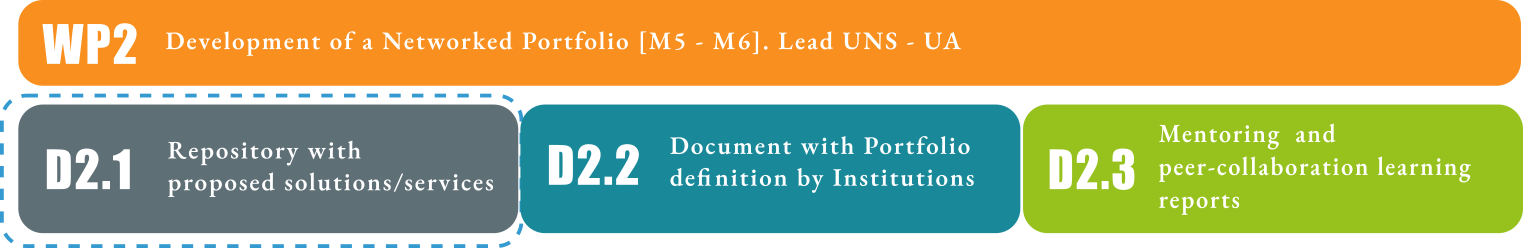
\includegraphics[keepaspectratio,alt={alt}]{figures/2.1/D2.1.png}}

}

\caption{\label{fig-baseline}WP2 baseline for TechTraplastiCE Project}

\end{figure}%

\chapter{Connection with WP1 Innovation Opportunities for Circular
Economy}\label{connection-with-wp1-innovation-opportunities-for-circular-economy}

Work Package 2 (WP2) builds directly on the analytical and empirical
results generated in Work Package 1 (WP1), included in deliverables
D1.1, D1.2, and D1.3. These deliverables provided a comprehensive and
multidimensional diagnosis of the regulatory frameworks, industrial
structures, and innovation capabilities that shape the circular economy
of plastics in Argentina, Chile, and Colombia. WP1 establishes a
systemic understanding of the context in each region, identifying key
barriers, stakeholders, and structural dynamics. On the other hand, WP2
seeks to identify, through a structured and operational mapping of the
institutional capacities of each consortium member, the knowledge that
can help key stakeholders overcome these barriers. In this sense, WP2
represents a crucial transition from diagnosis to action, enabling the
operationalization of university-industry collaboration through
concrete, structured, and deployable results. Rather than remaining at
the level of analysis, WP2 helps bridge the gap between knowledge
generation and implementation by organizing institutional competencies
into practical categories that can directly address the challenges
identified in WP1.

\section{From Regulatory and Institutional Diagnosis
(D1.1)}\label{from-regulatory-and-institutional-diagnosis-d1.1}

WP1 identified that Chile, Colombia and Argentina have developed
regulatory frameworks addressing plastic waste management and circular
economy principles. However, these frameworks differ significantly in
terms of implementation capacity, institutional coordination, and
enforcement mechanisms.

Chile stands out for its relatively consolidated legal framework,
supported by measurable targets and structured implementation
mechanisms. Colombia demonstrates rapid progress in policy integration,
particularly in relation to the inclusion of recycling actors and the
development of extended producer responsibility schemes. Argentina, on
the other hand, shows strong industrial and productive capabilities, but
faces challenges related to fragmented governance structures and limited
policy articulation across jurisdictions.

Across these three contexts, a set of common systemic barriers was
identified, including:

\begin{itemize}
\tightlist
\item
  Weak enforcement mechanisms that limit the effectiveness of existing
  regulations;
\item
  Limited economic incentives to promote circular practices;
\item
  Lack of traceability systems to monitor material flows;
\item
  Insufficient coordination between public institutions, private actors,
  and civil society.
\end{itemize}

These constraints define the operational environment in which WP2 is
implemented. In response, WP2 focuses on identifying and structuring
university-based services and capacities that can actively contribute to
overcoming these barriers. In particular, WP2 seeks to support the
implementation of regulatory frameworks through technical advisory and
scientific services; strengthen coordination mechanisms by mapping and
activating institutional engagement structures; and provide technical,
analytical, and organizational support to stakeholders involved in the
plastics value chain.

Through this approach, WP2 positions universities as key intermediaries
capable of supporting policy implementation and fostering more coherent
and effective governance systems.

\subsection{From value chain and systemic innovation analysis
(D1.2)}\label{from-value-chain-and-systemic-innovation-analysis-d1.2}

WP1 highlighted key structural characteristics of the plastics value
chain such as a strong dependence on a limited set of polymers
(polyethylene, polypropylene, polyvinyl chloride and polystyrene), a
concentration of industrial activities in specific sectors, and the
central role of packaging, construction, and agriculture as primary
areas of application.

The transition towards a circular economy in this context requires more
than isolated technological solutions. It demands systemic innovation
processes that involve the reconfiguration of interactions between
actors, as well as the integration of technological, social, and
institutional dimensions.

A particularly relevant finding concerns the role of recyclers,
especially informal actors, who play a critical role in material
recovery but remain insufficiently integrated into formal value chains.
This highlights the need for inclusive and systemic approaches that
recognize and strengthen these actors within the circular economy
ecosystem.

In this context, WP2 addresses these challenges by mapping institutional
capacities that are relevant for supporting circular economy
implementation across the value chain; identifying and structuring
training activities targeted at diverse stakeholders, including SMEs,
public institutions, and recycling actors; as well as organizing applied
research outputs that can contribute to both technological innovation
(e.g., materials, processes) and organizational innovation (e.g.,
business models, coordination mechanisms).

Through this approach, WP2 contributes to enabling systemic innovation
by linking knowledge production with practical applications and
stakeholder needs.

\subsection{From Innovation Capacity Assessment
(D1.3)}\label{from-innovation-capacity-assessment-d1.3}

The assessment conducted in WP1 regarding innovation capacities within
companies revealed significant asymmetries across the industrial
landscape. Large companies tend to demonstrate stronger innovation
performance, supported by greater access to resources, infrastructure,
and strategic capabilities. In contrast, SMEs and micro-enterprises show
considerable weaknesses, including limited access to technology, reduced
capacity for R\&D, and lower levels of integration into innovation
ecosystems. These findings underscore the need for targeted support
mechanisms that can enhance the innovation capacity of smaller actors,
which are nonetheless essential components of the plastics value chain.

In addition, WP1 facilitated the creation of a direct interface between
academia and industry, identifying concrete opportunities for
collaboration and applied research. WP2 builds on these results by:

\begin{itemize}
\tightlist
\item
  Aligning institutional service offerings and training programs with
  the specific needs of SMEs;
\item
  Structuring accessible technological services that lower barriers to
  innovation adoption;
\item
  Supporting the development of long-term university--industry
  partnerships, based on trust, complementarities, and shared
  objectives.
\end{itemize}

In this sense, WP2 contributes to democratizing access to knowledge and
technology, reinforcing the role of universities as enablers of
inclusive innovation.

\section{Operational mapping: from WP1 barriers to WP2
components}\label{operational-mapping-from-wp1-barriers-to-wp2-components}

To ensure a coherent and traceable transition from diagnosis to action,
WP2 translates the findings of WP1 into four operational categories:
services, capacities, developments, and training. This categorization
allows us for a systematic organization of institutional contributions
and facilitates their alignment with identified needs and gaps.

Table~\ref{tbl-link} illustrates this operational strategy, establishing
a direct link between the barriers identified in WP1 and the
corresponding WP2 components designed to address them. This mapping
ensures that the activities developed within WP2 are not only
theoretically grounded but also strategically oriented towards solving
concrete challenges within the plastics circular economy.

\begingroup\fontsize{11}{13}\selectfont

\begin{longtable}[t]{>{\raggedright\arraybackslash}p{5cm}>{\raggedright\arraybackslash}p{2cm}>{\raggedright\arraybackslash}p{4.5cm}>{\raggedright\arraybackslash}p{4cm}}

\caption{\label{tbl-link}Operational link between WP1 findings and WP2
components.}

\tabularnewline

\toprule
\begingroup\fontsize{12}{14}\selectfont \cellcolor{Naranja}{\textcolor{white}{\textbf{WP1 Identified Barrier / Gap}}}\endgroup & \begingroup\fontsize{12}{14}\selectfont \cellcolor{Naranja}{\textcolor{white}{\textbf{Source}}}\endgroup & \begingroup\fontsize{12}{14}\selectfont \cellcolor{Naranja}{\textcolor{white}{\textbf{WP2 Category}}}\endgroup & \begingroup\fontsize{12}{14}\selectfont \cellcolor{Naranja}{\textcolor{white}{\textbf{Operationalization}}}\endgroup\\
\midrule
\endfirsthead
\multicolumn{4}{@{}l}{\textit{(continued)}}\\
\toprule
\begingroup\fontsize{12}{14}\selectfont \cellcolor{Naranja}{\textcolor{white}{\textbf{WP1 Identified Barrier / Gap}}}\endgroup & \begingroup\fontsize{12}{14}\selectfont \cellcolor{Naranja}{\textcolor{white}{\textbf{Source}}}\endgroup & \begingroup\fontsize{12}{14}\selectfont \cellcolor{Naranja}{\textcolor{white}{\textbf{WP2 Category}}}\endgroup & \begingroup\fontsize{12}{14}\selectfont \cellcolor{Naranja}{\textcolor{white}{\textbf{Operationalization}}}\endgroup\\
\midrule
\endhead

\endfoot
\bottomrule
\endlastfoot
Weak policy implementation & D1.1 & Services / Capacities & Technical advisory and support services\\
\midrule\addlinespace
Lack of traceability & D1.1 & Developments / Services & Analytical tools and characterization services\\
\midrule\addlinespace
Limited coordination & D1.1 & Capacities & Mapping of institutional engagement structures\\
\midrule\addlinespace
Regulatory fragmentation & D1.1 & Training / Services & Training and advisory support\\
\midrule\addlinespace
Low adoption of circular practices & D1.1 / D1.2 & Services / Training & Industry-oriented services and training\\
\midrule\addlinespace
Limited innovation in materials & D1.2 & Developments & Identification of applied R\&D outputs\\
\midrule\addlinespace
Weak recycler integration & D1.2 & Training / Services & Inclusive training approaches\\
\midrule\addlinespace
SME innovation gaps & D1.3 & Training / Services & Capacity-building and technical support\\
\midrule\addlinespace
Limited access to technology & D1.3 & Services / Capacities & Access to infrastructure and expertise\\*

\end{longtable}

\endgroup{}

\section{Functional translation into WP2
categories}\label{functional-translation-into-wp2-categories}

Within WP2, institutional contributions are organized into four
complementary axes:

\begin{figure}[H]

{\centering 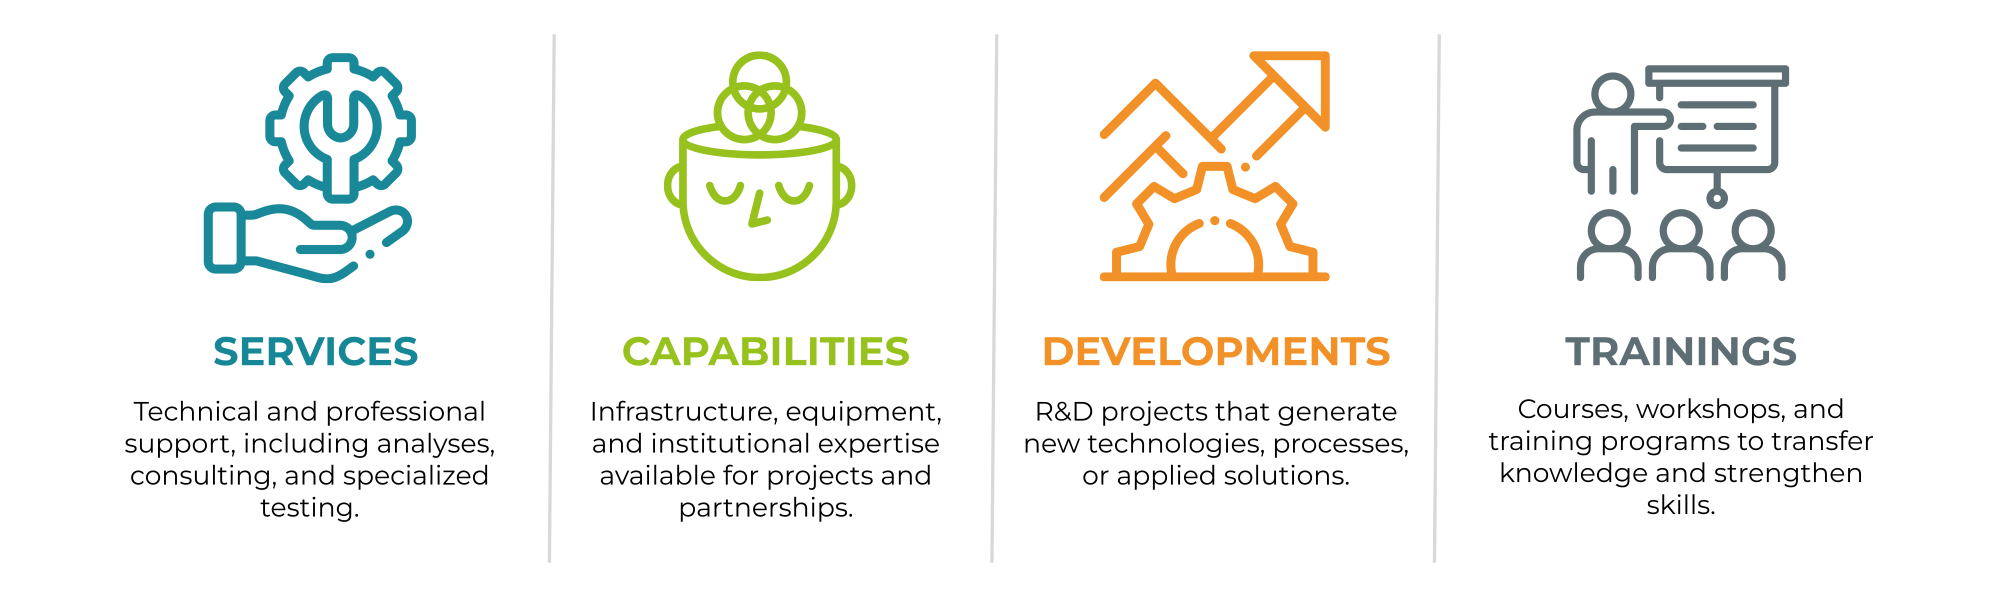
\includegraphics[width=0.85\linewidth,height=\textheight,keepaspectratio]{figures/2.1/Methodology-02.png}

}

\caption{Complementary axes of the institutional portfolio}

\end{figure}%

\begin{itemize}
\tightlist
\item
  \textbf{Services}: referring to technical and scientific services that
  address the immediate and practical needs of socio-economic actors;
\item
  \textbf{Capabilities:} encompassing institutional competencies,
  expertise, and available infrastructure;
\item
  \textbf{Developments}: including applied research outputs and
  technological solutions with transfer potential at different levels of
  maturity;
\item
  \textbf{Training}: covering educational and capacity-building
  activities targeting a wide range of stakeholders.
\end{itemize}

This structured approach enables a comprehensive representation of the
role of universities, capturing both their existing capabilities and
their potential contributions to the circular economy.

\section{Integration through the Canvas
Methodology}\label{integration-through-the-canvas-methodology}

The canvas-based workshop complements this mapping by providing
a~\textbf{co-creation mechanism}~that:

\begin{itemize}
\tightlist
\item
  Captures institution-specific insights;
\item
  Identifies current and future capacities;
\item
  Supports the identification of collaboration opportunities.
\end{itemize}

Each canvas dimension reflects WP1 findings, including:

\begin{enumerate}
\def\labelenumi{\arabic{enumi}.}
\tightlist
\item
  Institutional coordination challenges (institutional engagement
  strategies);
\item
  Innovation gaps (capabilities and applied R\&D results);
\item
  Inclusion challenges (training and barriers and opportunities).
\end{enumerate}

\section{From diagnosis to
operationalization}\label{from-diagnosis-to-operationalization}

WP1 provides the diagnostic framework, while WP2 transforms this
diagnosis into structured institutional responses. This transition
enables:

\begin{itemize}
\tightlist
\item
  The development of institutional portfolios;
\item
  The implementation of progressive technology transfer mechanisms;
\item
  The preparation of collaborative actions in subsequent work packages.
\end{itemize}

\section{Connection with future Work Packages 3 and
4}\label{connection-with-future-work-packages-3-and-4}

The outputs generated within WP2 serve as a critical baseline for the
development of subsequent work packages. In particular, they provide the
necessary inputs for the design and refinement of institutional
portfolios; the development of targeted training programs; and the
implementation of pilot collaboration initiatives between universities
and external stakeholders.

By structuring and systematizing institutional capacities, WP2
establishes the empirical and operational foundation upon which WP3 and
WP4 can build. It ensures that subsequent activities are grounded in a
clear understanding of available resources, competencies, and
opportunities for collaboration.

Ultimately, WP2 contributes to strengthening the coherence and
effectiveness of the project as a whole, enabling a coordinated and
strategic progression from mapping and analysis to implementation and
impact.

\chapter{Global methodology}\label{global-methodology}

The methodological approach adopted in WP2 is based on a comprehensive
mixed-method design that integrates structured quantitative-oriented
data collection with qualitative, participatory, and iterative
processes. This approach has been specifically conceived to respond to
the complexity of mapping technology transfer capacities across a
heterogeneous, multi-institutional, and transnational consortium.

\begin{figure}[H]

\centering{

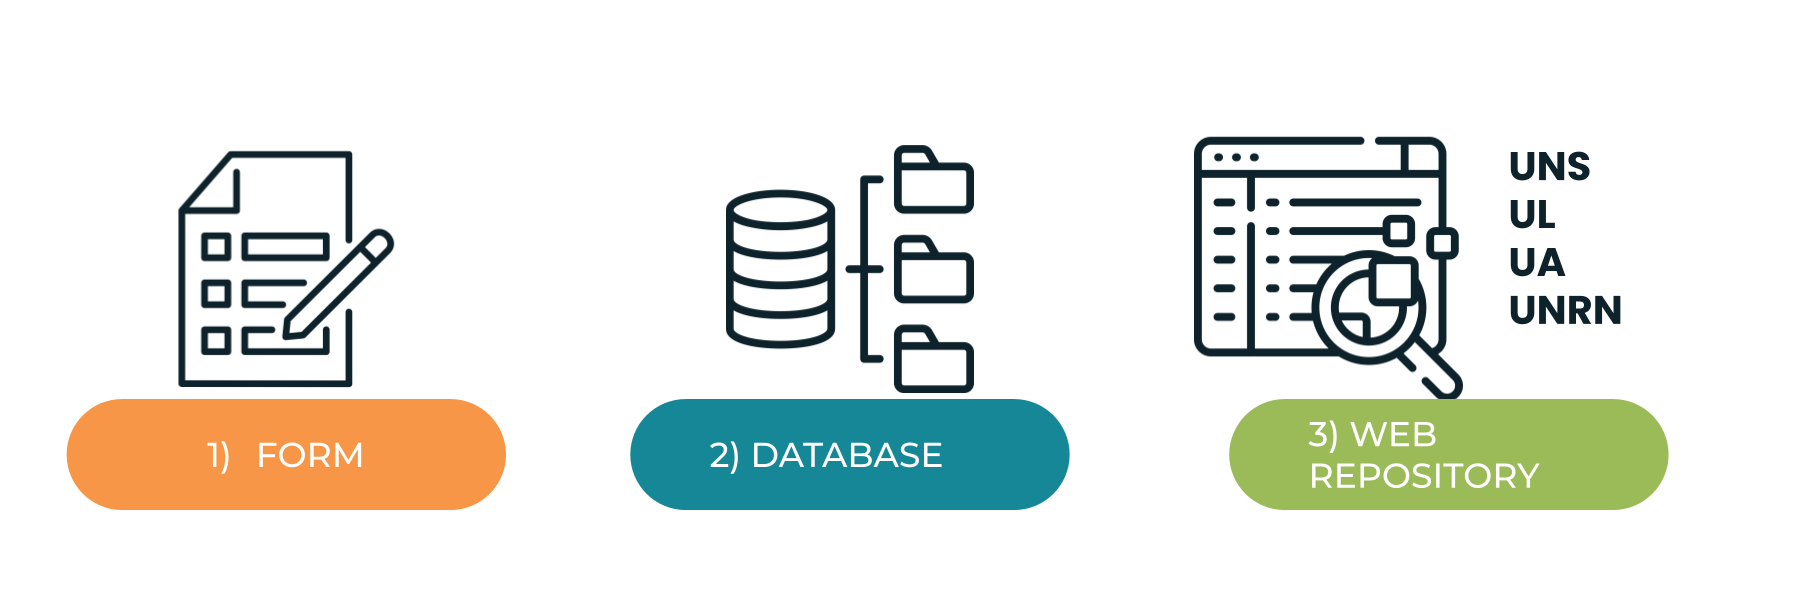
\includegraphics[width=0.8\linewidth,height=\textheight,keepaspectratio]{figures/2.1/Methodology-01.png}

}

\caption{\label{fig-method01}Global methodology of the WP2}

\end{figure}%

Given the diversity of institutional profiles, levels of maturity in
technology transfer, and socio-economic contexts represented within the
project, a purely standardized or purely qualitative methodology would
have been insufficient. Therefore, WP2 adopts a hybrid methodological
framework that ensures both analytical rigor and contextual sensitivity,
enabling the generation of robust, comparable, and actionable results.

The methodology combines three main components as illustrated in
Figure~\ref{fig-method01}:

\begin{enumerate}
\def\labelenumi{\arabic{enumi}.}
\tightlist
\item
  Structured questionnaires for systematic data collection;
\item
  An iterative data collection and validation process;
\item
  A participatory canvas-based workshop for co-creation and qualitative
  enrichment.
\end{enumerate}

These components are not independent but function as interconnected
stages within a progressive methodological sequence, in which data is
continuously refined, validated, and contextualized. This integrated
approach enables the construction of a standardized and comparable
dataset across institutions and countries; the incorporation of
context-specific qualitative insights, capturing institutional
diversity; the progressive refinement and validation of information,
ensuring data quality and reliability; the active engagement of partner
institutions in the co-creation of knowledge; and the transformation of
dispersed institutional information into structured and operational
outputs.

Furthermore, this methodological design ensures a clear alignment with
the objectives of WP2, particularly in terms of supporting the
development of institutional portfolios and facilitating the transition
from diagnostic analysis (WP1) to operational implementation (WP3 and
WP4).

\section{Structured questionnaires}\label{structured-questionnaires}

Structured questionnaires were developed as the primary instrument for
data collection to systematically capture detailed and comparable
information on the technology transfer capacities of partner
institutions. They were designed to collect data across four core
dimensions that reflect the operational categories of WP2:

\begin{itemize}
\tightlist
\item
  \textbf{Capabilities}: Research and innovation activities, including
  applied research and technological development;
\item
  \textbf{Services}: Technology transfer mechanisms and services offered
  to external stakeholders;
\item
  \textbf{Trainings}: Capacity-building activities targeting different
  audiences;
\item
  \textbf{Developments}: Applied research activities and collaboration
  practices with socio-economic actors, including industry, public
  institutions, and civil society organizations.
\end{itemize}

The design of the questionnaires was established taking into account the
analytical framework assessed in WP1, ensuring coherence between the
diagnostic phase and the mapping of institutional capacities. In
addition, specific attention was given to aligning the structure of the
questionnaires with the final outputs expected in WP2, particularly the
construction of technology cards and institutional portfolios.

In this sense, Figure~\ref{fig-questionnaires} includes the Google
questionnaires for each axis .

\begin{figure}[H]

\centering{

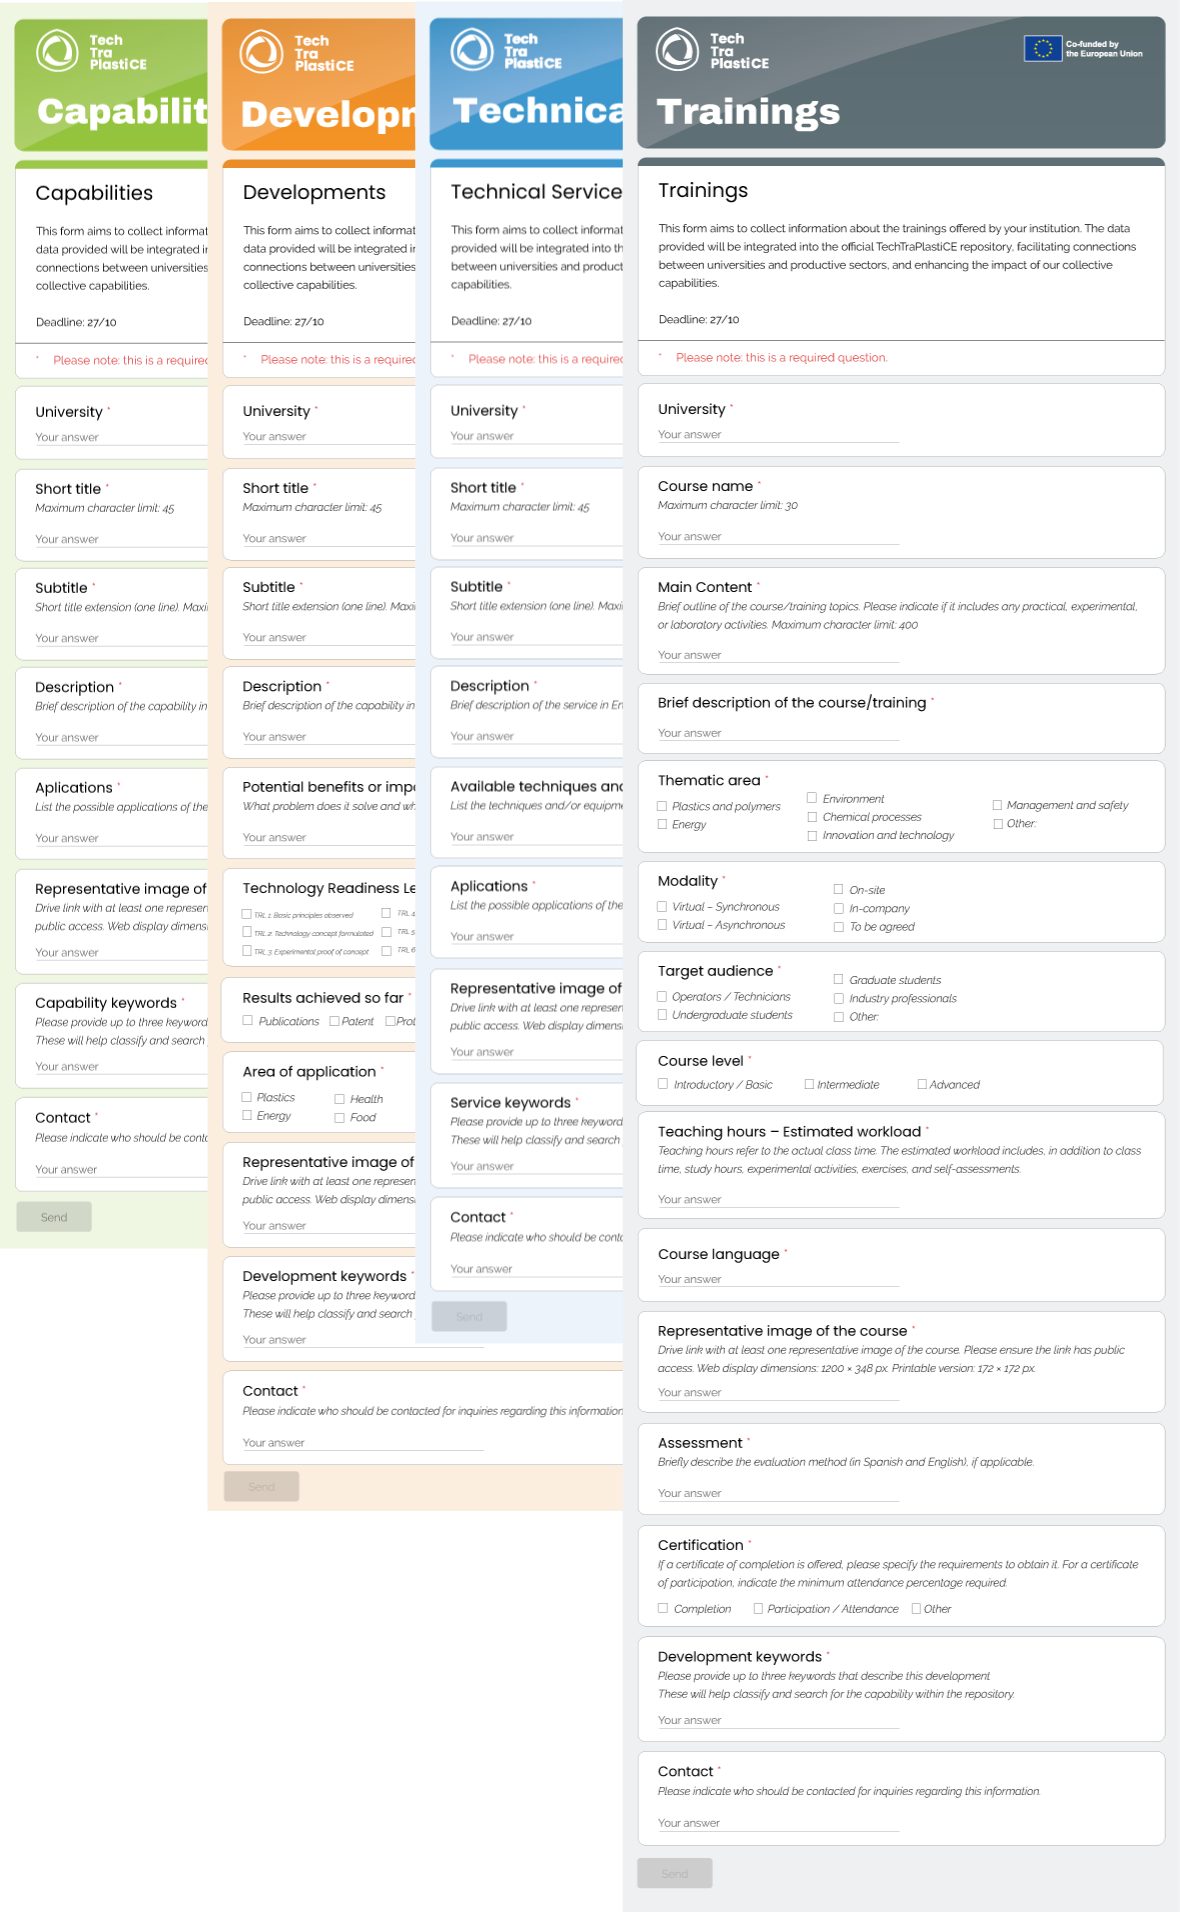
\includegraphics[width=0.75\linewidth,height=\textheight,keepaspectratio]{figures/2.1/Questionnaires.png}

}

\caption{\label{fig-questionnaires}Questionnaires for the complementary
axis: capabilities, developments, technical services and training.}

\end{figure}%

To support a consistent interpretation of the categories and ensure
methodological alignment across partners, the questionnaires were
complemented by a set of guidance materials. These included detailed
written instructions as well as explanatory videos specifically
developed for each category (services, capacities, developments, and
training). Although the slides in the videos are presented in English,
the audio is in Spanish, as it is the common working language among
consortium members. Figure~\ref{fig-videos} present the videos that can
be accessed through the following link:
\url{https://wp6.techtraplastice.eu/wp2-portfolio.html}

\begin{figure}[H]

\centering{

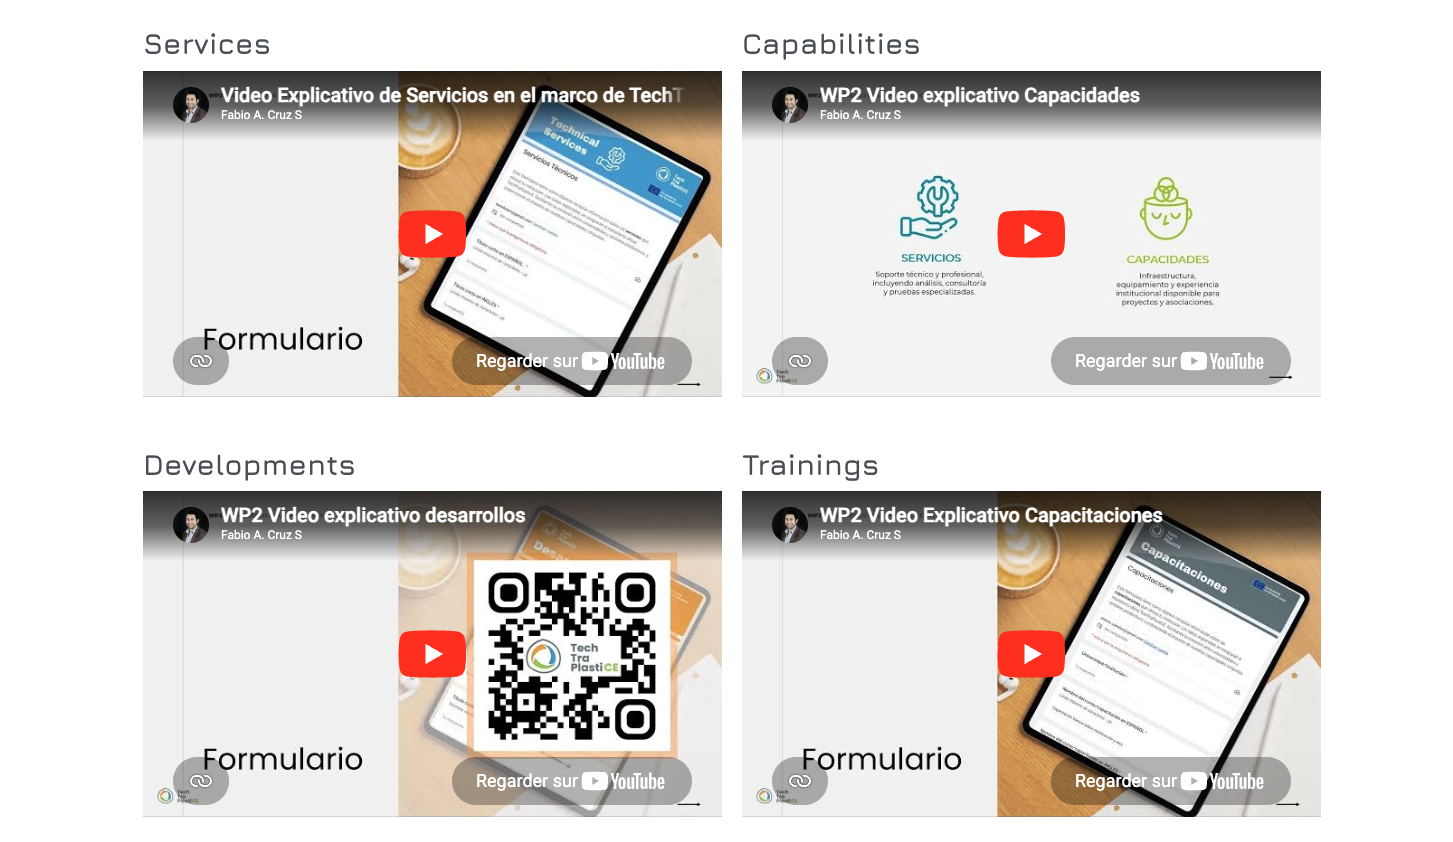
\includegraphics[width=0.8\linewidth,height=\textheight,keepaspectratio]{figures/2.1/Videos.png}

}

\caption{\label{fig-videos}Videos to support the common understanding of
the Questionnaires.}

\end{figure}%

The incorporation of video-based guidance represents a key
methodological innovation within WP2. These videos provided clear
definitions and conceptual boundaries for each category; practical
examples illustrating how to complete the forms; clarifications on
common sources of confusion or overlap between categories; and
step-by-step instructions for completing the questionnaires. This
multimodal guidance approach proved to be particularly valuable in a
context characterized by linguistic diversity (Spanish, Portuguese and
English), different institutional cultures, and dispair levels of
familiarity with technology transfer processes. It contributed
significantly to reducing interpretation biases and improving the
overall consistency of the data collected.

The structured nature of the questionnaires ensured a high degree of
comparability across institutions, enabling cross-case analysis; a
comprehensive coverage of key thematic areas relevant to the circular
economy of plastics; and a consistent format that facilitates subsequent
coding, categorization, and analysis. Through these questionnaires,
institutions were able to provide detailed descriptions of their
activities; highlight specific features or innovations; and reflect on
the potential applications and beneficiaries of their activities. The
timeline for respond the questionnaires was between \textbf{September
2025 - November 2025}.

\section{Iterative data collection
process}\label{iterative-data-collection-process}

The data collection process in WP2 was conceived as an iterative and
guided process, structured in four main stages. This iterative logic was
fundamental to ensuring not only the completeness of the dataset but
also its quality, coherence, and alignment with the methodological
framework.

\subsection{Step 1 -- Guidance and
Orientation}\label{step-1-guidance-and-orientation}

The process began with a comprehensive guidance phase, where partner
institutions were provided with all necessary materials to complete the
questionnaires. This included written instructions, methodological
guidelines, and explanatory videos tailored to each category. This
initial stage was critical to establishing a shared understanding of the
objectives, categories, and expected outputs. It also helped to align
partners with the conceptual framework of WP2 and to ensure consistency
from the outset of the data collection process.

\subsection{Step 2 -- Sequential Data
Entry}\label{step-2-sequential-data-entry}

Partners were instructed to complete the questionnaires following a
predefined sequence:

\begin{enumerate}
\def\labelenumi{\arabic{enumi}.}
\tightlist
\item
  Services (Mid Sept 2025 )
\item
  Capacities (Oct 205)
\item
  Developments (Mid Oct 2025)
\item
  Training (November 2025)
\end{enumerate}

This sequence was strategically defined to guide institutions through a
structured reflection process. Starting with services, typically more
visible and externally oriented, allowed institutions to identify their
immediate offerings. This was followed by capacities, which represent
the underlying resources and competencies that enable these services.
Subsequently, the focus shifted to developments, capturing applied
research outputs and technological innovations. Finally, training
activities were addressed, highlighting the role of institutions in
knowledge dissemination and capacity building. This approach not only
facilitated the data entry process but also encouraged institutions to
reflect on the internal coherence of their activities and the
relationships between different types of capacities. At the general
monthly meetings of the TechTraPlastiCE consortiums, there was the
oppportunity to answer quaestions and clarify the scope of the
questionnaires.

\subsection{Step 3 -- Submission, Review, and
Feedback}\label{step-3-submission-review-and-feedback}

Forms were submitted in both Spanish and English. The use of bilingual
submissions ensured inclusivity while also requiring additional
attention to consistency and comparability. Following submission, a
systematic internal review process was carried out. This process
included:

\begin{itemize}
\tightlist
\item
  Verification of data completeness;
\item
  Assessment of internal consistency across entries;
\item
  Review of the categorization assigned to each case;
\item
  Identification of potential overlaps or misclassifications;
\item
  Evaluation of clarity and quality of descriptions.
\end{itemize}

Where inconsistencies or ambiguities were identified, feedback was
provided to the corresponding institutions, initiating a revision
process. This feedback loop constitutes a key element of the iterative
methodology, allowing for continuous improvement of the dataset. This
stage ensured that the information used for subsequent analysis was not
only complete but also coherent and aligned with the project's
methodological criteria. Conclusions of this step are included in the
D2.2.

\subsection{Step 4 -- Timeline and Process
Coordination}\label{step-4-timeline-and-process-coordination}

The data collection process was conducted between October and early
December 2025. This period was carefully planned to allow sufficient
time for data entry, review, feedback, and revision, while maintaining
alignment with the overall project timeline. Throughout this phase,
continuous communication was maintained with partner institutions,
providing support, resolving doubts, and ensuring adherence to
deadlines. This active coordination contributed to a high level of
participation and data completeness across the consortium.

\section{Workshop and canvas-based
methodology}\label{workshop-and-canvas-based-methodology}

A consortium workshop held in Chile implemented a canvas-based
co-creation exercise (Figure~\ref{fig-canva}), designed to capture
additional qualitative insights, identify existing gaps and future
opportunities, and support the co-design of institutional portfolios.

\begin{figure}[H]

\centering{

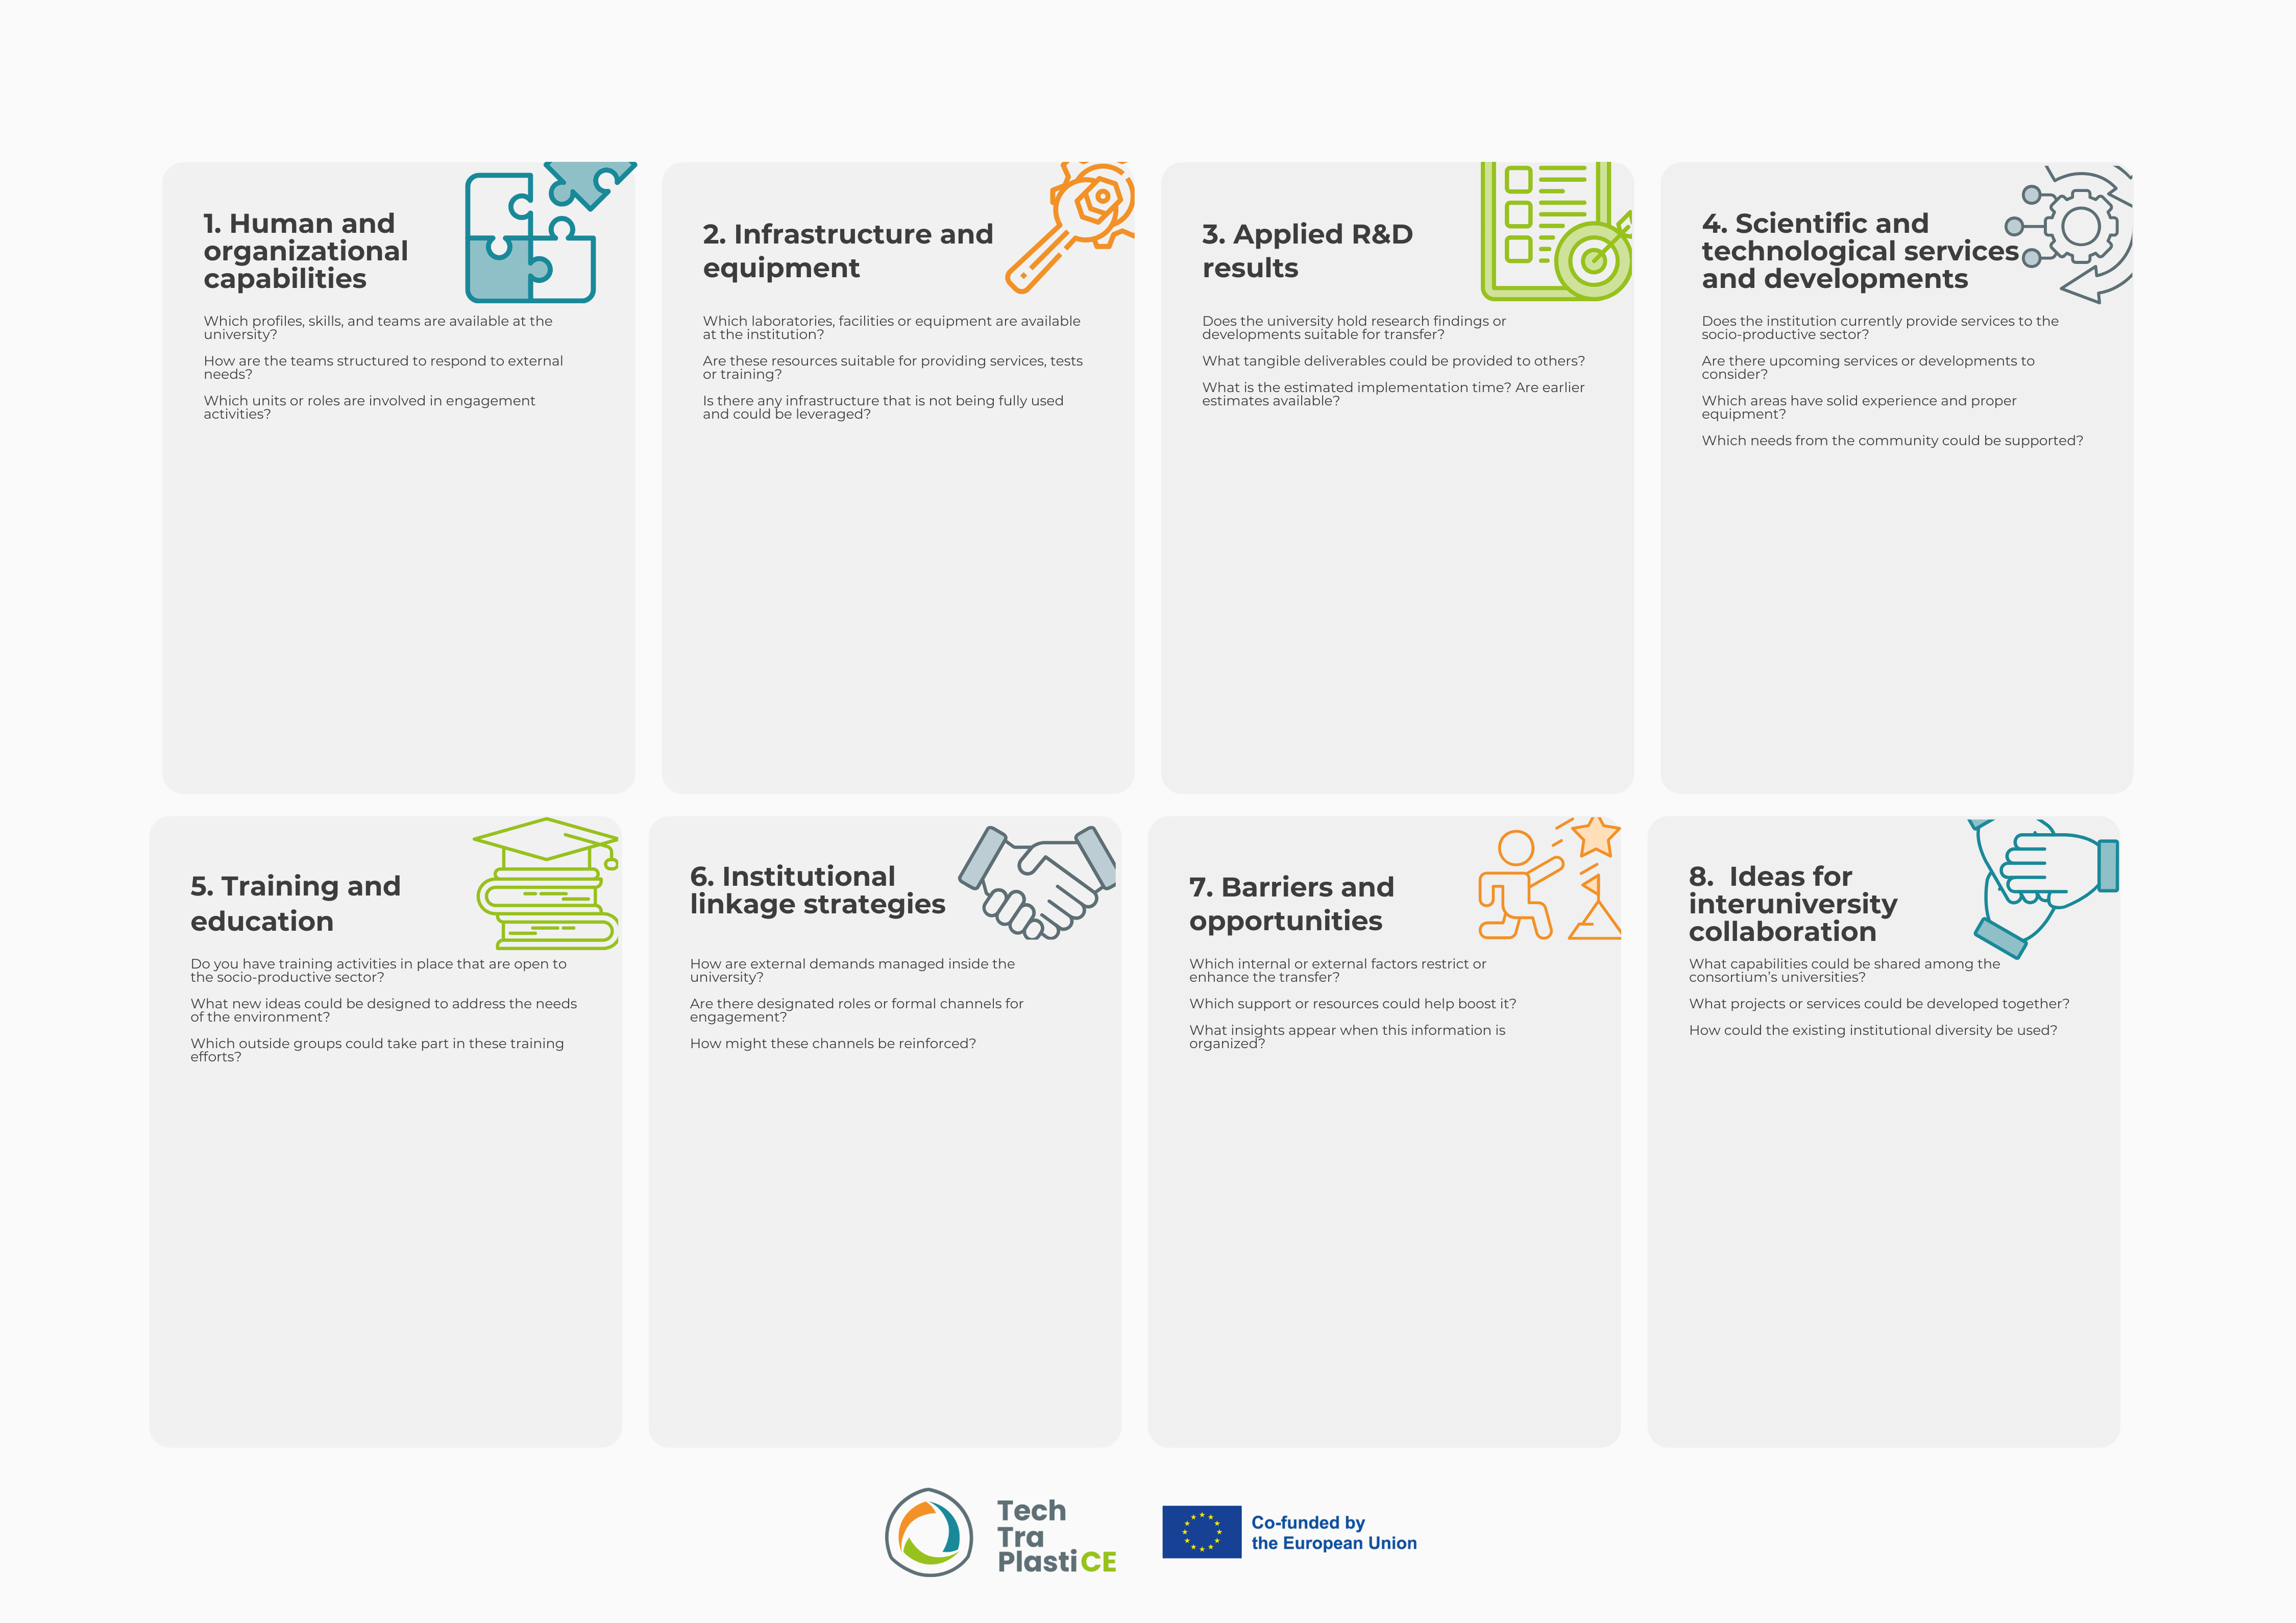
\includegraphics[width=1\linewidth,height=\textheight,keepaspectratio]{figures/2.1/Canva.png}

}

\caption{\label{fig-canva}Canva used at the workshop at the meeting
consortium in Chile Nov 2025}

\end{figure}%

The canvas was organized into eight dimensions: i) human and
organizational capabilities; ii) infrastructure and equipment; iii)
applied R\&D results; iv) scientific and technological services and
developments; v) training and education; vi) institutional engagement
strategies; vii) barriers and opportunities; and viii) ideas for
inter-university collaboration. Each dimension was explored through
guiding questions and collective discussion. The outputs generated
through this exercise were documented and integrated as complementary
qualitative data, enriching the structured dataset built through the
questionnaires as illustrated in Figure~\ref{fig-chile}. Obtained
results from this activity complemented the analysis carried out in the
following deliverables (D2.2 and D2.3).

\begin{figure}[H]

\centering{

\includegraphics[width=0.6\linewidth,height=\textheight,keepaspectratio]{figures/2.1/Chile.jpg}

}

\caption{\label{fig-chile}Face-to-face workshop on the Canva of at the
meeting consortium in Chile Nov 2025}

\end{figure}%

\section{Methodological Contribution to WP2
Objectives}\label{methodological-contribution-to-wp2-objectives}

Beyond its role in data collection, the methodological approach adopted
in WP2 contributes directly to the broader objectives of the work
package. By combining structured data with participatory processes, it
enables the transformation of fragmented information into structured
knowledge; the identification of institutional strengths and
complementarities; the development of comparable and operational
institutional portfolios; and the preparation of the consortium for
subsequent collaborative and implementation phases. In this sense, the
methodology is not only a technical tool but also a strategic instrument
that supports the transition from analysis to action within the project.

\chapter{Data collected}\label{data-collected}

The data collected within WP2 comprises both structured and qualitative
inputs, reflecting the mixed-method approach adopted throughout the work
package. Figure~\ref{fig-worldcloud} illustrates the major keywords of
the dataset. On the one hand, raw data was systematically gathered
through the structured questionnaires completed by all member
universities. These responses constitute the primary dataset, capturing
detailed information across the four core dimensions defined in WP2
(services, capacities, developments, and training). As illustrated in
Table~\ref{tbl-developments}, Table~\ref{tbl-capabilities},
Table~\ref{tbl-technical} and Table~\ref{tbl-training}, the collected
data is presented in tabular format to ensure clarity, comparability,
and traceability across institutions. Full access to these tables was
provided for the consortium repository. In the annexes
Section~\ref{sec-A2}, the complete raw data is plotted for the four
questionnaires.

\begin{figure}[H]

\centering{

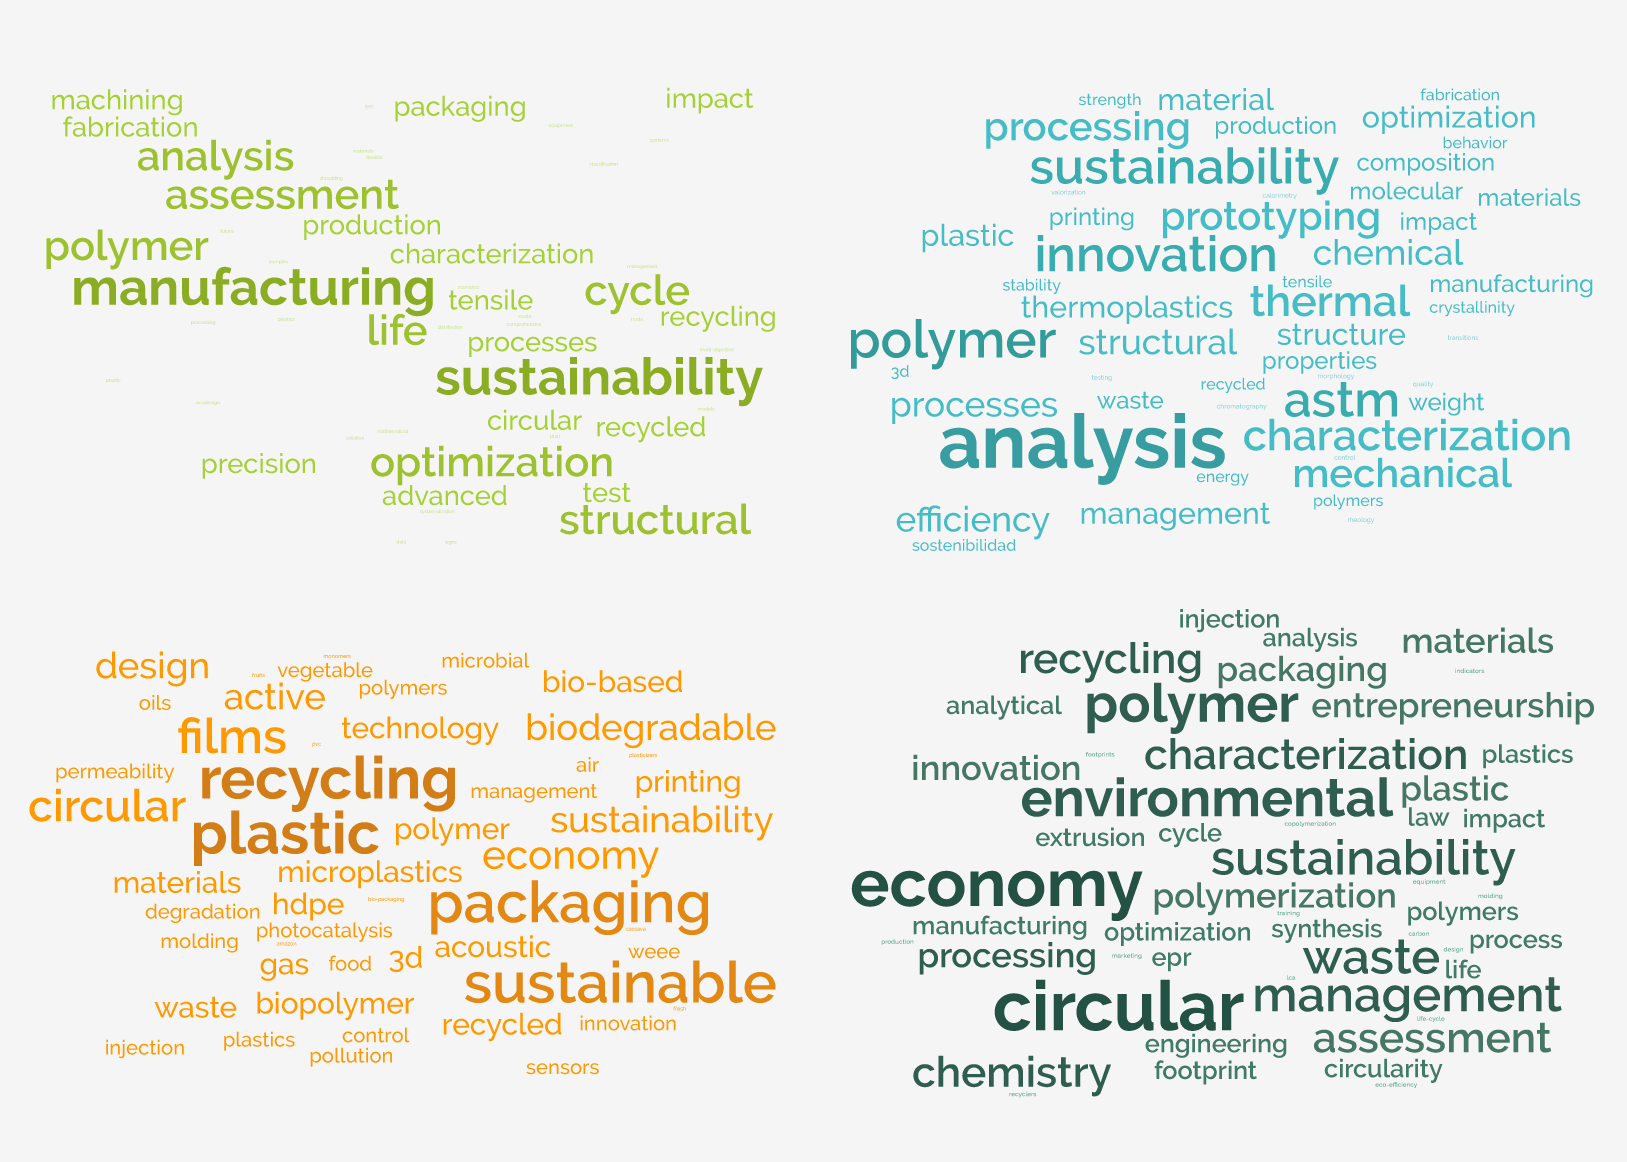
\includegraphics[width=0.75\linewidth,height=\textheight,keepaspectratio]{figures/2.1/worldcloud.png}

}

\caption{\label{fig-worldcloud}Wordcloud of the collected data using the
major related words (\emph{title}) the complementary axis: capabilities,
developments, technical services and training.}

\end{figure}%

\begin{landscape}

\section{Developments at each HEIs}\label{developments-at-each-heis}

\setlength{\tabcolsep}{2pt}
\renewcommand{\arraystretch}{0.75}

\begingroup\fontsize{7}{9}\selectfont

\begin{longtable}[t]{>{\raggedright\arraybackslash}p{3cm}>{\raggedleft\arraybackslash}p{0.6cm}>{\raggedright\arraybackslash}p{5.5cm}>{\raggedright\arraybackslash}p{9.5cm}}

\caption{\label{tbl-developments}Primary dataset of
\textbf{Developments} at each HEI. Complete dataset is found in the
Annex}

\tabularnewline

\toprule
\begingroup\fontsize{7}{9}\selectfont \cellcolor{Naranja}{\textcolor{white}{\textbf{HEI}}}\endgroup & \begingroup\fontsize{7}{9}\selectfont \cellcolor{Naranja}{\textcolor{white}{\textbf{ID}}}\endgroup & \begingroup\fontsize{7}{9}\selectfont \cellcolor{Naranja}{\textcolor{white}{\textbf{Title-EN}}}\endgroup & \begingroup\fontsize{7}{9}\selectfont \cellcolor{Naranja}{\textcolor{white}{\textbf{Subtitle-EN}}}\endgroup\\
\midrule
\endfirsthead
\multicolumn{4}{@{}l}{\textit{(continued)}}\\
\toprule
\begingroup\fontsize{7}{9}\selectfont \cellcolor{Naranja}{\textcolor{white}{\textbf{HEI}}}\endgroup & \begingroup\fontsize{7}{9}\selectfont \cellcolor{Naranja}{\textcolor{white}{\textbf{ID}}}\endgroup & \begingroup\fontsize{7}{9}\selectfont \cellcolor{Naranja}{\textcolor{white}{\textbf{Title-EN}}}\endgroup & \begingroup\fontsize{7}{9}\selectfont \cellcolor{Naranja}{\textcolor{white}{\textbf{Subtitle-EN}}}\endgroup\\
\midrule
\endhead

\endfoot
\bottomrule
\endlastfoot
 & 40 & Waste Transformation Prototypes & Development of materials from recycled pla, mdf and cardboard\\
\cmidrule{2-4}\nopagebreak
 & 41 & Ceramic pellets for 3D printing & Ceramic pellets for fdm printing of telecom antennas\\
\cmidrule{2-4}\nopagebreak
 & 42 & Waste Collection Optimization Platform & Optimizes routes and waste management for municipalities\\
\cmidrule{2-4}\nopagebreak
 & 43 & Autonomous Beach Cleaning Vehicle & Efficient autonomous prototype for beach waste collection\\
\cmidrule{2-4}\nopagebreak
 & 44 & Anticorrosive polymer with metal nanoparticles & Polymeric coating with metal nanoparticles against biocorrosion\\
\cmidrule{2-4}\nopagebreak
 & 45 & Method to detect microplastics & Identify and quantify microplastics in organic samples\\
\cmidrule{2-4}\nopagebreak
 & 46 & Microplastics baseline in sediment & Chronological method to track plastics in valparaíso bay\\
\cmidrule{2-4}\nopagebreak
 & 47 & Bacterial bioplastic and degradation & Development and biodegradability of phbv polymer\\
\cmidrule{2-4}\nopagebreak
\multirow[t]{-9}{3cm}[8\dimexpr\aboverulesep+\belowrulesep+\cmidrulewidth]{\raggedright\arraybackslash Pontificia Universidad Católica de Valparaíso (PUCV)} & 48 & PUCV plastic recycling machine & Machine to shred and mold recycled plastic\\
\cmidrule{1-4}\pagebreak[0]
Universidad Central & 38 & Bioplastic Development & Bioplastic prototype analysis\\
\cmidrule{1-4}\pagebreak[0]
 & 2 & Environmental Micro-Architecture & Architectural component for high-rise facades with the capacity to remove atmospheric pollution\\
\cmidrule{2-4}\nopagebreak
 & 3 & Plastic Architecture & Brick-type architectural component made from upcycled recycled hdpe plastic with environmental functions\\
\cmidrule{2-4}\nopagebreak
 & 4 & Photocatalytic HDPE Cladding & Slat-type cladding made from recycled hdpe for degradation of atmospheric pollutants\\
\cmidrule{2-4}\nopagebreak
 & 5 & SUMI Panel & Acoustic panel manufactured from hdpe plastic waste\\
\cmidrule{2-4}\nopagebreak
 & 6 & Recycled Plastic Acoustic Resonator & Recycled plastic acoustic resonator for workspaces\\
\cmidrule{2-4}\nopagebreak
 & 7 & Juan Fernández Circular & Prototyping useful products from recycled plastics for the juan fernández archipelago community\\
\cmidrule{2-4}\nopagebreak
 & 8 & PALF: Modular Photovoltaic Tile & Self-sufficient lighting system using recycled plastic and solar energy for critical campus areas\\
\cmidrule{2-4}\nopagebreak
 & 9 & Virtual recycling plant for circular economy learning & Interactive experience for understanding recycling processes and circular economy\\
\cmidrule{2-4}\nopagebreak
 & 10 & AI virtual teaching assistants for innovation courses & Intelligent support for learning creativity and innovation\\
\cmidrule{2-4}\nopagebreak
 & 11 & Local plastic recycling for additive manufacturing & Applied circular economy in innovation spaces\\
\cmidrule{2-4}\nopagebreak
 & 12 & Circular economy management in companies & Integrating circularity into organizational processes\\
\cmidrule{2-4}\nopagebreak
 & 13 & Sustainable innovation project management methodologies & Structuring and managing innovation projects through agile and sustainability-driven approaches\\
\cmidrule{2-4}\nopagebreak
 & 14 & Sustainable design of common pool resource supply chains & Design and modeling approaches for the sustainable management of shared resources\\
\cmidrule{2-4}\nopagebreak
\multirow[t]{-14}{3cm}[13\dimexpr\aboverulesep+\belowrulesep+\cmidrulewidth]{\raggedright\arraybackslash Universidad de Santiago de Chile} & 15 & Sustainable innovation management & Strategic integration of sustainability, innovation and value creation in organizations and startups\\
\cmidrule{1-4}\pagebreak[0]
 & 33 & Production of bio-based monomers & Synthesis of monomers from vegetable oils and used cooking oil\\
\cmidrule{2-4}\nopagebreak
 & 34 & Bio-based plasticizers for PVC & Production of ester and epoxide plasticizers from vegetable oils\\
\cmidrule{2-4}\nopagebreak
 & 35 & Breathable biodegradable bag for fruits (Actipack) & Packaging with controlled gas transmission for fresh fruit export\\
\cmidrule{2-4}\nopagebreak
 & 36 & Biodegradable packaging & Flexible and rigid packaging from amazonian starch and agro-waste\\
\cmidrule{2-4}\nopagebreak
\multirow[t]{-5}{3cm}[4\dimexpr\aboverulesep+\belowrulesep+\cmidrulewidth]{\raggedright\arraybackslash Universidad Nacional de Colombia} & 37 & Active packaging with natural fibers & Biodegradable containers with natural microfibers and preservative compounds\\
\cmidrule{1-4}\pagebreak[0]
Universidad Nacional de Córdoba & 32 & Biodegradable Cellulose Foams & Development of cellulose insulating foams\\
\cmidrule{1-4}\pagebreak[0]
 & 31 & SEMMIoTicAR & Portable microfluidic sensor for environmental microplastics iot monitoring\\
\cmidrule{2-4}\nopagebreak
\multirow[t]{-2}{3cm}[1\dimexpr\aboverulesep+\belowrulesep+\cmidrulewidth]{\raggedright\arraybackslash Universidad Nacional de Río Negro} & 39 & Bioprospecting for polymer-degrading microorganisms & Development of microbial consortia that degrade common synthetic polymers for environmental bioremediation\\
\cmidrule{1-4}\pagebreak[0]
 & 16 & Plastics WEEE recycling & Value added of plastic from waste electrical and electronic equipment\\
\cmidrule{2-4}\nopagebreak
 & 17 & Sensors for Smart Packaging & Flexible graphene-based films for bacterial detection in meat\\
\cmidrule{2-4}\nopagebreak
 & 18 & Multilayer Mono-material Packaging & Multilayer polyolefin-based composite packaging with tailored properties\\
\cmidrule{2-4}\nopagebreak
 & 19 & Starch Films & Starch films with specific functionalities\\
\cmidrule{2-4}\nopagebreak
 & 20 & Polymer Blends & Extrusion, injection and blow molding of tailored thermoplastic blends\\
\cmidrule{2-4}\nopagebreak
 & 21 & Polyhydroxyalkanoates PHAs & Biosynthesis of polyhydroxyalkanoates and copolymers\\
\cmidrule{2-4}\nopagebreak
 & 22 & Plastic WEEE Recycling & Added value to plastic waste from electrical and electronic equipment\\
\cmidrule{2-4}\nopagebreak
 & 23 & Plastic Paper & Writable, printable and paintable polyolefin plastic films\\
\cmidrule{2-4}\nopagebreak
 & 24 & Plastic Packaging with Prolonged Repellent Activity & Flexible active packaging with repellent controlled release\\
\cmidrule{2-4}\nopagebreak
 & 25 & New Materials for MAP & Materials with regulated permeability for packaging under modified atmosphere (map)\\
\cmidrule{2-4}\nopagebreak
 & 26 & Glyphosate Containers Recycling & Sustainable process for recycling plastic glyphosate containers\\
\cmidrule{2-4}\nopagebreak
 & 27 & Fuels From Plastics & Fuel production by thermal cracking of waste plastics\\
\cmidrule{2-4}\nopagebreak
 & 28 & Flexible Polymer Packaging & Flexible thermo sealed packaging for fresh fruits preservation without refrigeration\\
\cmidrule{2-4}\nopagebreak
 & 29 & Films for Fruits Dehydration & Fruits dehydration using biodegradable films with selective gases permeability\\
\cmidrule{2-4}\nopagebreak
\multirow[t]{-15}{3cm}[14\dimexpr\aboverulesep+\belowrulesep+\cmidrulewidth]{\raggedright\arraybackslash Universidad Nacional del Sur} & 30 & Biopolymeric Coatings & Biopolymeric coatings formulations with customized functionalities\\
\cmidrule{1-4}\pagebreak[0]
Universidade de Aveiro & 1 & Sustainable recycling of Expanded Polystyrene & Sustainable recycling of expanded polystyrene from packaging\\*

\end{longtable}

\endgroup{}

\newpage

\section{Capabilities at each HEIs}\label{capabilities-at-each-heis}

\begingroup\fontsize{7}{9}\selectfont

\begin{longtable}[t]{>{\raggedright\arraybackslash}p{3cm}>{\raggedleft\arraybackslash}p{0.6cm}>{\raggedright\arraybackslash}p{5.5cm}>{\raggedright\arraybackslash}p{9.5cm}}

\caption{\label{tbl-capabilities}Primary dataset of
\textbf{Capabilities} at each HEI. Complete dataset is found in the
Annex}

\tabularnewline

\toprule
\begingroup\fontsize{7}{9}\selectfont \cellcolor{Verde}{\textcolor{white}{\textbf{HEI}}}\endgroup & \begingroup\fontsize{7}{9}\selectfont \cellcolor{Verde}{\textcolor{white}{\textbf{ID}}}\endgroup & \begingroup\fontsize{7}{9}\selectfont \cellcolor{Verde}{\textcolor{white}{\textbf{Title-EN}}}\endgroup & \begingroup\fontsize{7}{9}\selectfont \cellcolor{Verde}{\textcolor{white}{\textbf{Subtitle-EN}}}\endgroup\\
\midrule
\endfirsthead
\multicolumn{4}{@{}l}{\textit{(continued)}}\\
\toprule
\begingroup\fontsize{7}{9}\selectfont \cellcolor{Verde}{\textcolor{white}{\textbf{HEI}}}\endgroup & \begingroup\fontsize{7}{9}\selectfont \cellcolor{Verde}{\textcolor{white}{\textbf{ID}}}\endgroup & \begingroup\fontsize{7}{9}\selectfont \cellcolor{Verde}{\textcolor{white}{\textbf{Title-EN}}}\endgroup & \begingroup\fontsize{7}{9}\selectfont \cellcolor{Verde}{\textcolor{white}{\textbf{Subtitle-EN}}}\endgroup\\
\midrule
\endhead

\endfoot
\bottomrule
\endlastfoot
 & 74 & Polymer Laboratory & Synthesis and study of materials with technological potential\\
\cmidrule{2-4}\nopagebreak
 & 75 & Polymer Laboratory & Synthesis and study of materials with technological potential\\
\cmidrule{2-4}\nopagebreak
 & 76 & Electron Microscopy Laboratory & Advanced microstructural and elemental characterization\\
\cmidrule{2-4}\nopagebreak
 & 77 & Valparaíso Makerspace: creative, tech \& collaborative space & Space equipped for the creation, validation and testing of prototypes.\\
\cmidrule{2-4}\nopagebreak
\multirow[t]{-5}{3cm}[4\dimexpr\aboverulesep+\belowrulesep+\cmidrulewidth]{\raggedright\arraybackslash Pontificia Universidad Católica De Valparaíso} & 78 & PUCV Institutional Recycling System & Comprehensive waste management and traceability\\
\cmidrule{1-4}\pagebreak[0]
 & 55 & Technical Support in Plastic Classification & Applied testing for innovation in recycling and recycled plastic material (rpm) processing\\
\cmidrule{2-4}\nopagebreak
 & 56 & Urban Waste Management Modeling & Mathematical models for trend and scenario analysis\\
\cmidrule{2-4}\nopagebreak
 & 57 & Formulation of Comprehensive Waste Management Plans (PGIRS) & Analysis of plastic packaging waste management\\
\cmidrule{2-4}\nopagebreak
 & 58 & Logistics Optimization & Development and application of route optimization models\\
\cmidrule{2-4}\nopagebreak
 & 59 & Equipment Assistance, Maintenance, and Operation & Training and technical advisory to improve equipment use and useful life\\
\cmidrule{2-4}\nopagebreak
 & 60 & Process Optimization in the Manufacturing Industry & Consulting for productive efficiency in the plastics sector\\
\cmidrule{2-4}\nopagebreak
 & 61 & Plastic Prototype Analysis & Evaluation of plastic prototypes under injection parameters\\
\cmidrule{2-4}\nopagebreak
 & 62 & Circular Policy Assessment & Support for knowledge and implementation of circular economy policies\\
\cmidrule{2-4}\nopagebreak
 & 63 & Life Cycle Assessment Consulting & Life cycle analysis of plastic materials and processes\\
\cmidrule{2-4}\nopagebreak
 & 64 & Plastic Compatibility Study & Analysis of plastic waste compatibility for material testing\\
\cmidrule{2-4}\nopagebreak
 & 65 & Technical Advisory Services for Recyclers & Support and guidance in technical skill development for recyclers\\
\cmidrule{2-4}\nopagebreak
 & 66 & Analysis of Synthetic Polymers & Identification of synthetic polymers through characterization techniques\\
\cmidrule{2-4}\nopagebreak
 & 67 & Intellectual and Industrial Property & Advisory services in intellectual and industrial property for problem-solving\\
\cmidrule{2-4}\nopagebreak
 & 68 & Technological Development of Instrumentation & Support in instrumentation design\\
\cmidrule{2-4}\nopagebreak
\multirow[t]{-15}{3cm}[14\dimexpr\aboverulesep+\belowrulesep+\cmidrulewidth]{\raggedright\arraybackslash Universidad Central} & 69 & Circularity Adoption Pathways & Methodologies for adopting circularity within esg indicators\\
\cmidrule{1-4}\pagebreak[0]
 & 14 & Innovation project management methodologies (Design Thinking, Lean Startup, etc.) & A comparative framework for guiding sustainable and market-driven innovation processes\\
\cmidrule{2-4}\nopagebreak
 & 15 & Ability to generate solutions with a focus on innovation & Driving creative problem-solving through strategic and user-centered approaches\\
\cmidrule{2-4}\nopagebreak
 & 16 & Innovative solution prototyping & Design, modeling and early validation of solutions through functional prototypes\\
\cmidrule{2-4}\nopagebreak
 & 17 & Business model development & Designing value-driven, scalable and sustainable organizational architectures\\
\cmidrule{2-4}\nopagebreak
 & 18 & Assessment of innovation capacity in companies & Evaluating organizational enablers, barriers and readiness for sustained innovation\\
\cmidrule{2-4}\nopagebreak
 & 19 & Innovation capability diagnosis for compaines & Strategic assessment of organizational innovation maturity\\
\cmidrule{2-4}\nopagebreak
 & 20 & Capabilities in Design and Prototyping from Mechanical Recycling of Plastics & Interdisciplinary development of sustainable materials and architectural prototypes through the mechanical processing of recycled polymers.\\
\cmidrule{2-4}\nopagebreak
 & 21 & Immersive Training in Circular Economy for Plastics through Virtual Reality & Experiential learning on recycling and sustainability through interactive virtual environments\\
\cmidrule{2-4}\nopagebreak
 & 22 & Sustainable Innovation Indicator for Companies & Measure, evaluate, and strengthen your company’s innovative and sustainable capabilities.\\
\cmidrule{2-4}\nopagebreak
 & 23 & Design and Development of Architectural Products Using Recycled Plastic & Comprehensive solutions from design to prototyping and production\\
\cmidrule{2-4}\nopagebreak
 & 24 & Characterization of Plastics for Architecture and Construction & Analysis and characterization of materials based on mechanical, chemical, and thermal properties\\
\cmidrule{2-4}\nopagebreak
 & 25 & Environmental Impact Assessment & Evaluating environmental risks, sustainability performance and mitigation strategies\\
\cmidrule{2-4}\nopagebreak
 & 26 & Mathematical simulation of production systems & Modeling complex systems to predict behavior and optimize decision-making\\
\cmidrule{2-4}\nopagebreak
\multirow[t]{-14}{3cm}[13\dimexpr\aboverulesep+\belowrulesep+\cmidrulewidth]{\raggedright\arraybackslash Universidad de Santiago de Chile} & 27 & Solving circular logistics problems & Strategies to optimize resource loops, reverse flows and sustainable value recovery\\
\cmidrule{1-4}\pagebreak[0]
 & 49 & Design for sustainability & Development of sustainable products and processes\\
\cmidrule{2-4}\nopagebreak
 & 50 & Circularity assessment & Circularity assessment in process and products\\
\cmidrule{2-4}\nopagebreak
 & 51 & Sustainability analysis & Comprehensive assessment of environmental, social, and economic impact.\\
\cmidrule{2-4}\nopagebreak
 & 52 & Mechanical and thermal characterization of polymers & Integral analysis of mechanical and thermal\\
\cmidrule{2-4}\nopagebreak
 & 53 & Polymerization processes & Custom polymer design and synthesis for specific applications\\
\cmidrule{2-4}\nopagebreak
\multirow[t]{-6}{3cm}[5\dimexpr\aboverulesep+\belowrulesep+\cmidrulewidth]{\raggedright\arraybackslash Universidad Nacional De Colombia} & 54 & Polymer process scale-up & Modeling and scaling of processes\\
\cmidrule{1-4}\pagebreak[0]
 & 46 & Polymer blend processing and formulation capabilities & Development and optimization of polymer compounds at laboratory and pilot scale\\
\cmidrule{2-4}\nopagebreak
 & 47 & Comprehensive polymer characterization capability & Physicochemical, thermal, mechanical and morphological characterization of polymers\\
\cmidrule{2-4}\nopagebreak
\multirow[t]{-3}{3cm}[2\dimexpr\aboverulesep+\belowrulesep+\cmidrulewidth]{\raggedright\arraybackslash Universidad Nacional De Córdoba} & 48 & Polymer processing capability with high-pressure fluids & Modification of polymer properties using supercritical fluids\\
\cmidrule{1-4}\pagebreak[0]
 & 45 & SEMMIOTICAR & Comprehensive approach to measuring and remedying microplastic pollution\\
\cmidrule{2-4}\nopagebreak
 & 70 & Support for the circular economy & Support and strengthening of intermediary entities in the circular economy\\
\cmidrule{2-4}\nopagebreak
 & 71 & Environmental management plan & Environmental management plan at atlantic site of unrn\\
\cmidrule{2-4}\nopagebreak
 & 72 & Design of recycling systems & Design of local recycling systems with social inclusion\\
\cmidrule{2-4}\nopagebreak
\multirow[t]{-5}{3cm}[4\dimexpr\aboverulesep+\belowrulesep+\cmidrulewidth]{\raggedright\arraybackslash Universidad Nacional De Río Negro} & 73 & Environmental Quality and Biotechnology Laboratory (LCAB) & R\&d\&i in biotechnology applied to environmental sustainability.\\
\cmidrule{1-4}\pagebreak[0]
 & 28 & Polymer Processing & Thermoplastic composites/nanocomposites processing operations experience\\
\cmidrule{2-4}\nopagebreak
 & 29 & Evaluation of Finished Packaging & Failure analysis of food and pharmaceutical packaging, migration and compliance tests\\
\cmidrule{2-4}\nopagebreak
 & 30 & Wastewater Treatment & Treatment of phenolic and aniline-related compounds from wastewaters\\
\cmidrule{2-4}\nopagebreak
 & 31 & Energy Efficiency & Reduction of energy consumption\\
\cmidrule{2-4}\nopagebreak
 & 32 & Environmental Studies & Evaluation and implementation of analytical methods\\
\cmidrule{2-4}\nopagebreak
 & 33 & Bioplastics Process Modeling & Superstructure-based optimization model for biopolymer production processes\\
\cmidrule{2-4}\nopagebreak
 & 34 & Biorefinery Design \& Optimization & Decision making insights for integrated biorefinery through mathematical modeling\\
\cmidrule{2-4}\nopagebreak
 & 35 & Engineering and Consulting & Process engineering services\\
\cmidrule{2-4}\nopagebreak
 & 36 & Plastic Film with Tailored Surface & Thermoplastic films with tailor-made surface by a process without adhesives\\
\cmidrule{2-4}\nopagebreak
 & 37 & Composite/ Nanocomposite Processing & Thermoplastic composites/nanocomposites processing operations experience\\
\cmidrule{2-4}\nopagebreak
 & 38 & Tailored Polymer Processes & Model-based design of polymer synthesis, degradation and post-reactor processes\\
\cmidrule{2-4}\nopagebreak
 & 39 & Polymer Synthesis & Controlled macromolecular synthesis\\
\cmidrule{2-4}\nopagebreak
 & 40 & Plastic Products & Evaluation of finished plastic products\\
\cmidrule{2-4}\nopagebreak
 & 41 & Materials Identification & Separation and identification of components by physical and chemical methods\\
\cmidrule{2-4}\nopagebreak
 & 42 & Plastic Materials Characterization & Complete characterization of polymer physicochemical properties\\
\cmidrule{2-4}\nopagebreak
 & 43 & Flexible Packaging Materials & Performance and failure analysis of polymeric packaging materials\\
\cmidrule{2-4}\nopagebreak
\multirow[t]{-17}{3cm}[16\dimexpr\aboverulesep+\belowrulesep+\cmidrulewidth]{\raggedright\arraybackslash Universidad Nacional Del Sur} & 44 & Failure and Contamination Analysis & Evaluation of polymers, blends, composites, films and laminates\\
\cmidrule{1-4}\pagebreak[0]
 & 1 & Barrier and surface properties & Analysis of barrier and surface properties of polymers\\
\cmidrule{2-4}\nopagebreak
 & 2 & Morphological characterization of plastic materials & Micro- and nanoscale analysis of virgin, recycled, composite, and nanocomposite polymers\\
\cmidrule{2-4}\nopagebreak
 & 3 & Optical properties of polymers & Uv-vis characterization and colorimetric analysis\\
\cmidrule{2-4}\nopagebreak
 & 4 & Rheological properties of polymers & Rheological properties of polymers\\
\cmidrule{2-4}\nopagebreak
 & 5 & Thermal analysis of polymers & Thermal characterization using tga, dsc, dta, conductivity and diffusivity\\
\cmidrule{2-4}\nopagebreak
 & 6 & Plastic surface coating & Development and study of functional coatings applied by screen printing, doctor blade coating, and spray coating\\
\cmidrule{2-4}\nopagebreak
 & 7 & Mechanical properties of plastic materials & Evaluation of mechanical properties through tensile, compression, flexural, hardness, and impact testing\\
\cmidrule{2-4}\nopagebreak
 & 8 & Structural analysis of polymeric materials & Advanced capabilities for studying chemical structure, crystallinity and degradation in polymeric materials\\
\cmidrule{2-4}\nopagebreak
 & 9 & Design of thermoplastic compounds & Development and optimization of thermoplastic and functional compounds with real-time rheological control.\\
\cmidrule{2-4}\nopagebreak
 & 10 & Polymer extrusion & Development of circular formulations and functional compounds at lab and pilot scale via single- and twin-screw extrusion\\
\cmidrule{2-4}\nopagebreak
 & 11 & 3D printing of thermoplastic materials & Development, parameterization, and validation of thermoplastic materials for additive manufacturing at laboratory scale.\\
\cmidrule{2-4}\nopagebreak
 & 12 & Injection molding of thermoplastic polymers & Processing and validation of thermoplastic polymers, blends, and composites at laboratory and pilot scale.\\
\cmidrule{2-4}\nopagebreak
\multirow[t]{-13}{3cm}[12\dimexpr\aboverulesep+\belowrulesep+\cmidrulewidth]{\raggedright\arraybackslash Universidade De Aveiro} & 13 & Thermocompression of thermoplastic polymers & Molding of sheets and films by hot pressing.\\*

\end{longtable}

\endgroup{}

\newpage

\section{Technical Services at each
HEIs}\label{technical-services-at-each-heis}

\begingroup\fontsize{7}{9}\selectfont

\begin{longtable}[t]{>{\raggedright\arraybackslash}p{2.5cm}>{\raggedleft\arraybackslash}p{0.6cm}>{\raggedright\arraybackslash}p{5.5cm}>{\raggedright\arraybackslash}p{9.5cm}}

\caption{\label{tbl-technical}Primary dataset of \textbf{Technical
Services} at each HEI. Complete dataset is found in the Annex}

\tabularnewline

\toprule
\begingroup\fontsize{7}{9}\selectfont \cellcolor{Celeste}{\textcolor{white}{\textbf{HEI}}}\endgroup & \begingroup\fontsize{7}{9}\selectfont \cellcolor{Celeste}{\textcolor{white}{\textbf{ID}}}\endgroup & \begingroup\fontsize{7}{9}\selectfont \cellcolor{Celeste}{\textcolor{white}{\textbf{Title-EN}}}\endgroup & \begingroup\fontsize{7}{9}\selectfont \cellcolor{Celeste}{\textcolor{white}{\textbf{Subtitle-EN}}}\endgroup\\
\midrule
\endfirsthead
\multicolumn{4}{@{}l}{\textit{(continued)}}\\
\toprule
\begingroup\fontsize{7}{9}\selectfont \cellcolor{Celeste}{\textcolor{white}{\textbf{HEI}}}\endgroup & \begingroup\fontsize{7}{9}\selectfont \cellcolor{Celeste}{\textcolor{white}{\textbf{ID}}}\endgroup & \begingroup\fontsize{7}{9}\selectfont \cellcolor{Celeste}{\textcolor{white}{\textbf{Title-EN}}}\endgroup & \begingroup\fontsize{7}{9}\selectfont \cellcolor{Celeste}{\textcolor{white}{\textbf{Subtitle-EN}}}\endgroup\\
\midrule
\endhead

\endfoot
\bottomrule
\endlastfoot
 & 98 & Product development and innovation & Support in the formulation and execution of r\&d\&i projects\\
\cmidrule{2-4}\nopagebreak
 & 99 & Environmental consulting and sustainability & Advisory on sustainability, circular economy, and environmental management\\
\cmidrule{2-4}\nopagebreak
 & 100 & Materials Testing & Structural testing to characterize the behavior of materials and elements under load\\
\cmidrule{2-4}\nopagebreak
 & 101 & Gestión de huella de carbono e hídrica & Measurement, verification, and reduction of environmental footprints in organizations and projects.\\
\cmidrule{2-4}\nopagebreak
 & 102 & Energy efficiency and resource management & Diagnosis and optimization of energy consumption and efficient resource use.\\
\cmidrule{2-4}\nopagebreak
 & 103 & Circular economy and waste valorization & Development of sustainable solutions for waste and by-product valorization.\\
\cmidrule{2-4}\nopagebreak
 & 104 & R\&D\&I project formulation & Design of innovation and sustainability projects.\\
\cmidrule{2-4}\nopagebreak
 & 105 & Energy audit & Technical assessment of energy consumption in production processes.\\
\cmidrule{2-4}\nopagebreak
 & 106 & Chrysalis Incubation Services & Comprehensive support for innovative high-potential ventures and startups\\
\cmidrule{2-4}\nopagebreak
\multirow[t]{-10}{2.5cm}[9\dimexpr\aboverulesep+\belowrulesep+\cmidrulewidth]{\raggedright\arraybackslash Pontificia Universidad Católica De Valparaíso} & 107 & Municipal Climate Action Plans (PACCC) & Technical and methodological support for the development of local adaptation and mitigation plans.\\
\cmidrule{1-4}\pagebreak[0]
 & 77 & Thermal Behavior Testing in Plastics & Viscosity and temperature analysis in plastics\\
\cmidrule{2-4}\nopagebreak
 & 78 & Atomic Force Microscopy (AFM) & Atomic force microscopy (afm) testing for polymer quality\\
\cmidrule{2-4}\nopagebreak
 & 79 & Fourier Transform Infrared Spectroscopy (FTIR) & Ftir testing for characterization and quality assessment of recycled plastics\\
\cmidrule{2-4}\nopagebreak
 & 80 & Dynamic Light Scattering (DLS) & Particle size measurement testing in polymers\\
\cmidrule{2-4}\nopagebreak
 & 81 & Mechanical Performance Analysis & Evaluation of material behavior under mechanical indicators\\
\cmidrule{2-4}\nopagebreak
 & 82 & Polymer Analysis by Spectroscopy & Identification of synthetic polymers using spectroscopic techniques\\
\cmidrule{2-4}\nopagebreak
 & 83 & Plastic Prototypes by Injection Molding & Plastic prototype manufacturing through injection molding\\
\cmidrule{2-4}\nopagebreak
 & 84 & Technology Foresight & Technology surveillance and competitive intelligence\\
\cmidrule{2-4}\nopagebreak
 & 85 & Maintenance, Diagnostics, and Commissioning & Support in maintenance and assessment of equipment operational condition\\
\cmidrule{2-4}\nopagebreak
 & 86 & Ad Hoc Logistics Optimization & Development and implementation of route optimization models\\
\cmidrule{2-4}\nopagebreak
 & 87 & Market Studies & Market analysis to identify opportunities in the plastics industry\\
\cmidrule{2-4}\nopagebreak
 & 88 & Design Thinking & Guidance and support in the implementation of design thinking\\
\cmidrule{2-4}\nopagebreak
\multirow[t]{-13}{2.5cm}[12\dimexpr\aboverulesep+\belowrulesep+\cmidrulewidth]{\raggedright\arraybackslash Universidad Central} & 89 & Failure Analysis of Plastic Materials & Material behavior under critical variables\\
\cmidrule{1-4}\pagebreak[0]
 & 12 & Product and service prototyping advisory & Technical and methodological support for functional prototypes\\
\cmidrule{2-4}\nopagebreak
 & 13 & 3D modeling and printing & Physical prototype fabrication for early validation\\
\cmidrule{2-4}\nopagebreak
 & 14 & Juan Fernandez Circular & Development of a comprehensive technological system for solid waste management\\
\cmidrule{2-4}\nopagebreak
 & 15 & Innovation capability diagnosis for compaines & Strategic assessment of organizational innovation maturity\\
\cmidrule{2-4}\nopagebreak
 & 16 & Business model advisory & Design and validation of innovative business models\\
\cmidrule{2-4}\nopagebreak
 & 17 & Sustainable innovation management & Integrating sustainability into innovation processes\\
\cmidrule{2-4}\nopagebreak
 & 18 & Organizational and production process management & Optimization of organizational structures and processes\\
\cmidrule{2-4}\nopagebreak
 & 19 & Support in applying for entrepreneurship funds & Strategic support in funding application processes\\
\cmidrule{2-4}\nopagebreak
 & 20 & Organizational and production process management & Optimization of organizational structures and processes\\
\cmidrule{2-4}\nopagebreak
 & 21 & Recycled Plastics Prototyping & Additive manufacturing and pilot-scale prototyping for recycled product development\\
\cmidrule{2-4}\nopagebreak
 & 22 & Testing of Recycled Plastic Materials & Mechanical, thermal, and chemical characterization for performance assessment\\
\cmidrule{2-4}\nopagebreak
 & 23 & Recycling Project Formulation & Technical and conceptual design of recycling initiatives focused on materials and sustainability\\
\cmidrule{2-4}\nopagebreak
 & 24 & TRL Assessment and Validation & Technology maturity diagnosis and roadmap for scale-up and technology transfer\\
\cmidrule{2-4}\nopagebreak
 & 25 & PoC Validation and Commercial Scale-Up & Technical consulting to turn recycled-material prototypes into scalable products\\
\cmidrule{2-4}\nopagebreak
 & 26 & Creativity workshops for idea generation & Activating creative potential to generate actionable and viable ideas\\
\cmidrule{2-4}\nopagebreak
 & 27 & Agile methodology workshops for innovation project management & Agile approaches to manage innovation projects iteratively and customer-centrically\\
\cmidrule{2-4}\nopagebreak
 & 28 & Life Cycle Assessment and Carbon Footprint Analysis & Comprehensive environmental assessment of products, processes and production systems\\
\cmidrule{2-4}\nopagebreak
 & 29 & Optimization and simulation of production systems & Mathematical modeling for efficient and sustainable production decisions\\
\cmidrule{2-4}\nopagebreak
 & 30 & Sustainable production strategies & Strategic design of efficient and responsible production systems\\
\cmidrule{2-4}\nopagebreak
 & 31 & Education for sustainable production systems & Capacity building for sustainable work environments\\
\cmidrule{2-4}\nopagebreak
 & 32 & Sustainable procurement and bidding analysis & Technical support for sustainable procurement processes\\
\cmidrule{2-4}\nopagebreak
 & 33 & Prioritization of sustainable production actions & Strategic prioritization to maximize impact and efficiency\\
\cmidrule{2-4}\nopagebreak
 & 34 & Sustainable operational optimization & Continuous improvement of production processes\\
\cmidrule{2-4}\nopagebreak
 & 35 & Scientific and technological project development & Formulation and execution of applied r\&d projects\\
\cmidrule{2-4}\nopagebreak
\multirow[t]{-25}{2.5cm}[24\dimexpr\aboverulesep+\belowrulesep+\cmidrulewidth]{\raggedright\arraybackslash Universidad De Santiago De Chile} & 36 & Recycled Plastics Application Consulting & Technical assessment for the use of recycled plastic products in architecture and design\\
\cmidrule{1-4}\pagebreak[0]
 & 55 & Polymer characterization & Polymer rheology\\
\cmidrule{2-4}\nopagebreak
 & 56 & Polymer rheological characterization & Cone and plate viscosity analysis\\
\cmidrule{2-4}\nopagebreak
 & 57 & Physical properties: water absorption & Determination of water absorption in plastics\\
\cmidrule{2-4}\nopagebreak
 & 58 & Physical properties: density & Density of plastics by displacement\\
\cmidrule{2-4}\nopagebreak
 & 59 & Physical properties: foam density & Apparent density of cellular plastics\\
\cmidrule{2-4}\nopagebreak
 & 60 & Durability: UV weathering & Accelerated weathering in uv chamber\\
\cmidrule{2-4}\nopagebreak
 & 61 & Fire behavior: horizontal burn & Horizontal burning test for plastics\\
\cmidrule{2-4}\nopagebreak
 & 62 & Surface properties: contact angle & Hydrophilic/hydrophobic analysis\\
\cmidrule{2-4}\nopagebreak
 & 63 & Microstructural analysis & Optical microscopy of materials\\
\cmidrule{2-4}\nopagebreak
 & 64 & Particle size analysis & Characterization of nanoparticles and emulsions\\
\cmidrule{2-4}\nopagebreak
 & 65 & Chromatographic analysis & Separation and quantification by hplc\\
\cmidrule{2-4}\nopagebreak
 & 66 & Optical properties: color & Color determination in plastic films\\
\cmidrule{2-4}\nopagebreak
 & 67 & Compositional analysis: ash content & Determination of inorganic content in plastics\\
\cmidrule{2-4}\nopagebreak
 & 68 & Mechanical properties: tension & Tensile testing of rigid plastics\\
\cmidrule{2-4}\nopagebreak
 & 69 & Mechanical properties: film tension & Tensile testing of thin films and sheeting\\
\cmidrule{2-4}\nopagebreak
 & 70 & Mechanical properties: flexure & Three-point bending test\\
\cmidrule{2-4}\nopagebreak
 & 71 & Mechanical properties: Shore A hardness & Hardness measurement in elastomers and rubbers\\
\cmidrule{2-4}\nopagebreak
 & 72 & Physical properties: thickness measurement & Dimensional control of films and coatings\\
\cmidrule{2-4}\nopagebreak
 & 73 & Mechanical properties: compression & Compression testing of rigid plastics\\
\cmidrule{2-4}\nopagebreak
 & 74 & Thermal analysis: DSC & Differential scanning calorimetry\\
\cmidrule{2-4}\nopagebreak
 & 75 & Thermal analysis: HP-DSC & High-pressure differential scanning calorimetry\\
\cmidrule{2-4}\nopagebreak
\multirow[t]{-22}{2.5cm}[21\dimexpr\aboverulesep+\belowrulesep+\cmidrulewidth]{\raggedright\arraybackslash Universidad Nacional De Colombia} & 76 & Thermal analysis: TGA & Thermogravimetric analysis\\
\cmidrule{1-4}\pagebreak[0]
 & 52 & Thermal analysis of polymers & Differential scanning calorimetry (dsc)\\
\cmidrule{2-4}\nopagebreak
 & 53 & Mechanical properties of polymers & Tensile, flexural, and impact tests to evaluate strength and stiffness\\
\cmidrule{2-4}\nopagebreak
\multirow[t]{-3}{2.5cm}[2\dimexpr\aboverulesep+\belowrulesep+\cmidrulewidth]{\raggedright\arraybackslash Universidad Nacional De Córdoba} & 54 & Biodegradability tests & Standardized polymer degradation analyses\\
\cmidrule{1-4}\pagebreak[0]
 & 51 & SEMMIoTicAR Sevices & Environmental microplastics iot monitoring\\
\cmidrule{2-4}\nopagebreak
 & 90 & Organizational analysis and diagnosis & Management, processes and human resources analysis  of the public institutions, third sector and companies\\
\cmidrule{2-4}\nopagebreak
 & 91 & Human resources management & Desing and implementation of human resource policies\\
\cmidrule{2-4}\nopagebreak
 & 92 & organizational management systems & Design and implementation of organizational management systems\\
\cmidrule{2-4}\nopagebreak
 & 93 & Strategic planning counseling & Development of strategic planning processes through workshops\\
\cmidrule{2-4}\nopagebreak
 & 94 & Analysis of microplastics (MPs) in aquatic ecosystems. & Identification and quantification of microplastics in aquatic ecosystems for environmental studies.\\
\cmidrule{2-4}\nopagebreak
 & 95 & Monitoring and analysis of microplastics & Detection and quantification in aquatic environmental matrices (abiotic and biotic)\\
\cmidrule{2-4}\nopagebreak
 & 96 & Strengthening Cooperatives & Strengthening cooperatives for waste recovery and recycling\\
\cmidrule{2-4}\nopagebreak
\multirow[t]{-9}{2.5cm}[8\dimexpr\aboverulesep+\belowrulesep+\cmidrulewidth]{\raggedright\arraybackslash Universidad Nacional De Río Negro} & 97 & Environmental Diagnosis & Comprehensive environmental assessment to improve sustainability\\
\cmidrule{1-4}\pagebreak[0]
 & 37 & Integral Characterization of Plastic Waste & Compositional analysis of plastic waste\\
\cmidrule{2-4}\nopagebreak
 & 38 & Weathering & Accelerated weathering tests under specific uv light, humidity and heat conditions\\
\cmidrule{2-4}\nopagebreak
 & 39 & Tribology & Wear and friction of polymeric materials\\
\cmidrule{2-4}\nopagebreak
 & 40 & Thermogravimetric analysis & Amount and rate of mass change as a function of temperature or time\\
\cmidrule{2-4}\nopagebreak
 & 41 & Rheology & Rheological characterization of polymeric materials\\
\cmidrule{2-4}\nopagebreak
 & 42 & Polymer Quality Control & Quality control of polymer raw materials and finished plastic products\\
\cmidrule{2-4}\nopagebreak
 & 43 & Polymer Processing & Evaluation of polymer processing behavior under lab and pilot plant scale\\
\cmidrule{2-4}\nopagebreak
 & 44 & Package/Food Interaction Analysis & Migration and compliance tests of food packaging\\
\cmidrule{2-4}\nopagebreak
 & 45 & Molecular Analysis & Molecular weights and mw distribution of polymers\\
\cmidrule{2-4}\nopagebreak
 & 46 & Microscopy & Structural and morphological analysis of materials\\
\cmidrule{2-4}\nopagebreak
 & 47 & Mechanical Performance & Mechanical evaluation of polymeric materials\\
\cmidrule{2-4}\nopagebreak
 & 48 & Infrared Spectroscopy & Quantitative and qualitative analysis for organic and inorganic samples\\
\cmidrule{2-4}\nopagebreak
 & 49 & Differential Scanning Calorimetry & Thermal analysis of polymeric materials\\
\cmidrule{2-4}\nopagebreak
\multirow[t]{-14}{2.5cm}[13\dimexpr\aboverulesep+\belowrulesep+\cmidrulewidth]{\raggedright\arraybackslash Universidad Nacional Del Sur} & 50 & Composting and Biodegradation & Evaluation of the biodegradability rate under controlled composting conditions\\
\cmidrule{1-4}\pagebreak[0]
 & 1 & Structural analysis of plastic materials & Structural characterisation using xrd, ftir, raman and complementary techniques.\\
\cmidrule{2-4}\nopagebreak
 & 2 & Mechanical testing of plastic materials & Evaluation of mechanical properties through tensile, compression, flexural, hardness, and impact testing\\
\cmidrule{2-4}\nopagebreak
 & 3 & Optical analysis of polymers & Optical analysis of polymers by uv-vis spectrometry and colorimetric analysis\\
\cmidrule{2-4}\nopagebreak
 & 4 & Plastic surface coating & Surface coating by screen printing, doctor blade coating, and spray coating\\
\cmidrule{2-4}\nopagebreak
 & 5 & Morphological analysis technical service & Micro- and nanoscale characterization of plastic materials using optical and electron microscopy techniques.\\
\cmidrule{2-4}\nopagebreak
 & 6 & Analysis of Barrier and surface properties & Determination of water vapor and oxygen permeability and contact angle measurement.\\
\cmidrule{2-4}\nopagebreak
 & 7 & Thermal analysis of polymers & Thermal analysis of polymers using thermogravimetric analysis, differential scanning calorimetry, and differential thermal analysis\\
\cmidrule{2-4}\nopagebreak
 & 8 & Polymer extrusion technical service & Continuous processing of thermoplastic and functional composite materials at lab and pilot scale\\
\cmidrule{2-4}\nopagebreak
 & 9 & 3D printing technical service & Additive manufacturing of thermoplastic and composite materials at laboratory scale.\\
\cmidrule{2-4}\nopagebreak
 & 10 & Injection molding techical service & Processing of thermoplastic, recycled, and composite materials at laboratory and pilot scale.\\
\cmidrule{2-4}\nopagebreak
 & 11 & Servicio de compounding & Blending and processing of thermoplastic and composite materials with rheological control.\\
\cmidrule{2-4}\nopagebreak
\multirow[t]{-12}{2.5cm}[11\dimexpr\aboverulesep+\belowrulesep+\cmidrulewidth]{\raggedright\arraybackslash Universidade De Aveiro} & 108 & Thermocompression service & Hot pressing of thermoplastic and composite materials.\\*

\end{longtable}

\endgroup{}

\newpage

\section{Training Programs at each
HEIs}\label{training-programs-at-each-heis}

\begingroup\fontsize{7}{9}\selectfont

\begin{longtable}[t]{>{\raggedright\arraybackslash}p{2cm}>{\raggedleft\arraybackslash}p{1cm}>{\raggedright\arraybackslash}p{3cm}>{\raggedright\arraybackslash}p{11cm}l}

\caption{\label{tbl-training}Primary dataset of \textbf{Training} at
each HEI. Complete dataset is found in the Annex}

\tabularnewline

\toprule
\begingroup\fontsize{7}{9}\selectfont \cellcolor{Neutro}{\textcolor{white}{\textbf{HEI}}}\endgroup & \begingroup\fontsize{7}{9}\selectfont \cellcolor{Neutro}{\textcolor{white}{\textbf{ID}}}\endgroup & \begingroup\fontsize{7}{9}\selectfont \cellcolor{Neutro}{\textcolor{white}{\textbf{Title-EN}}}\endgroup & \begingroup\fontsize{7}{9}\selectfont \cellcolor{Neutro}{\textcolor{white}{\textbf{Content-EN}}}\endgroup & \begingroup\fontsize{7}{9}\selectfont \cellcolor{Neutro}{\textcolor{white}{\textbf{Level}}}\endgroup\\
\midrule
\endfirsthead
\multicolumn{5}{@{}l}{\textit{(continued)}}\\
\toprule
\begingroup\fontsize{7}{9}\selectfont \cellcolor{Neutro}{\textcolor{white}{\textbf{HEI}}}\endgroup & \begingroup\fontsize{7}{9}\selectfont \cellcolor{Neutro}{\textcolor{white}{\textbf{ID}}}\endgroup & \begingroup\fontsize{7}{9}\selectfont \cellcolor{Neutro}{\textcolor{white}{\textbf{Title-EN}}}\endgroup & \begingroup\fontsize{7}{9}\selectfont \cellcolor{Neutro}{\textcolor{white}{\textbf{Content-EN}}}\endgroup & \begingroup\fontsize{7}{9}\selectfont \cellcolor{Neutro}{\textcolor{white}{\textbf{Level}}}\endgroup\\
\midrule
\endhead

\endfoot
\bottomrule
\endlastfoot
 & 1 & Bioplastics Resources and Technologies & Bioplastics Resources and Technologies is an university-accredited qualification to respond to new market needs by providing a tailor-made course to update and deepen the skills of persons working in companies possessing agri-food byproducts, and in companies producing formulations and bioplastics in different forms. & Advanced\\
\cmidrule{2-5}\nopagebreak
 & 2 & Sustainable Plastics - from feedstocks to product design & The Sustainable Plastics - from natural raw materials to product design course is a qualification accredited by the university to respond to new mobility opportunities, offering a mixed (virtual and face-to-face) intensive course to give students the opportunity to gain skills to implement an experimental project. & Medium\\
\cmidrule{2-5}\nopagebreak
\multirow[t]{-3}{2cm}[2\dimexpr\aboverulesep+\belowrulesep+\cmidrulewidth]{\raggedright\arraybackslash Universidade De Aveiro} & 3 & UACOOPERA - Cooperation and knowledge transfer & Fostering a culture of innovation and knowledge transfer, while supporting the academic community in addressing challenges and providing solutions for business and society in general. & Advanced\\
\cmidrule{1-5}\pagebreak[0]
 & 7 & Basic Training on Plastic Classification and Mechanical Recycling & The course covers basic topics such as what plastics are and how they behave under different conditions, and why it is important not to mix them. It also includes topics related to plastic classification using accessible techniques, fundamental concepts and criteria of mechanical recycling, and safety procedures to be considered during the process. In addition, the environmental role of sorting activities within the circular economy of these materials will be analyzed. & Introductory\\
\cmidrule{2-5}\nopagebreak
 & 8 & Polymer Testing Methods & Ad-hoc courses tailored to cover the specific needs of materials technologists, students, design engineers and researchers. The testing methods covered are focused on the characterization of the whole range of physical and chemical properties, including mechanical, optical, thermal, barrier and processability tests. & Introductory\\
\cmidrule{2-5}\nopagebreak
 & 9 & Polymer Processes & Ad-hoc courses for each interested party, tailored to its specific needs. Possible contents include: conventional and controlled free radical polymerization; Ziegler-Natta and metallocenic processes; stepwise polymerization; measurement and prediction of molecular weight distributions; copolymers; polymerizations in mass, suspension, emulsion, solution, gas-phase and other technologies; post-reactor modification: controlled rheology, functionalization, degradation, industrial examples of polymer processes. & Medium\\
\cmidrule{2-5}\nopagebreak
 & 10 & Macromolecular Architectures & Macromolecular architectures involve synthesis, design and development of tailor-made polymers by employing different synthetic methods. From conventional step-growth or chain-growth to latest controlled radical polymerizations, in this course different Polymer Science topics regarding the synthesis and characterization of complex macromolecular structures are covered. & Medium\\
\cmidrule{2-5}\nopagebreak
 & 11 & Gas Chromatography & Gas chromatography (GC) is a widely used analytical tool for qualitative and quantitative characterization of different samples. Examples of typical applications involving GC technique are analysis of natural products, food composition, food additives, flavor and aroma components, natural gas, a variety of transformation products, packaging materials and contaminants (such as environmental pollutants, fumigants pesticides and natural toxins). The course covers basic and practical aspects of handling GC. & Advanced\\
\cmidrule{2-5}\nopagebreak
 & 12 & Biopolymers & Biopolymers and biodegradable materials are proposed as alternative materials to synthetic polymers. They are finding new industrial and commercial applications: packaging, medical supplies, and automotive parts, among others. Thus, some aspects including obtaining methods, processing technologies, costs, environmental sustainability, characteristics, final properties, and developing products are relevant. This course gives an overview of the biopolymer field from the obtaining to characterization, properties, and applications of these materials. & Medium\\
\cmidrule{2-5}\nopagebreak
\multirow[t]{-7}{2cm}[6\dimexpr\aboverulesep+\belowrulesep+\cmidrulewidth]{\raggedright\arraybackslash Universidad Nacional Del Sur} & 37 & Basic training on plastic classification and mechanical recycling & The course covers basic topics such as what plastics are and how they behave under different conditions, and why it is important not to mix them. It also includes topics related to plastic classification using accessible techniques, fundamental concepts and criteria of mechanical recycling, and safety procedures to be considered during the process. In addition, the environmental role of sorting activities within the circular economy of these materials will be analyzed. & Introductory\\
\cmidrule{1-5}\pagebreak[0]
 & 24 & Environmental Education and Awareness Plan & The Plan has two stages: 1) theoretical and practical environmental education training, focused on promoting waste recycling as a healthy and strategic habit to encourage proper waste management, as well as strengthening and enhancing a circular and sustainable economy. The courses are geared towards different audiences and levels of complexity; 2) implementation of a pilot program within the institution for separating wet and dry waste for proper recycling. & Medium\\
\cmidrule{2-5}\nopagebreak
 & 25 & Environmental Impact of Plastics & Assessment of the fate and effects of plastics in aquatic ecosystems as an indicator of leakage in the circular economy. The interaction of microplastics with environmental matrices and their ecotoxicological impact on biota (macroinvertebrates and fish) are addressed. Environmental risk analysis is conducted to inform mitigation strategies and the redesign of sustainable production processes & Medium\\
\cmidrule{2-5}\nopagebreak
 & 26 & Training for middle and senior managers in management and leadership & Communication Power, Performance, and Reputation Leadership Time Management Agile Methodologies Effective Delegation Oral Presentations Analysis and Problem Solving High-Performance Team Management Conflict and Negotiation Change Management & Medium\\
\cmidrule{2-5}\nopagebreak
 & 27 & Metagenomics and Biotechnology for a Circular Economy & Introduction to microbial ecology and its application in the degradation and valorization of polymeric waste. Bioinformatics and metagenomics tools for studying the microbiome in impacted environments. Bioprospecting strategies to identify enzymes capable of degrading plastics. Bioeconomy and sustainable processes in industry. & Advanced\\
\cmidrule{2-5}\nopagebreak
\multirow[t]{-5}{2cm}[4\dimexpr\aboverulesep+\belowrulesep+\cmidrulewidth]{\raggedright\arraybackslash Universidad Nacional De Río Negro} & 28 & Entrepreneur training & Entrepreneurship, ideas, and business opportunities Business management Business Model Canvas Cost analysis Business plan Communication Time management and agile methodologies & Medium\\
\cmidrule{1-5}\pagebreak[0]
 & 13 & University Diploma in Circular Economy and Sustainability StrategiesEconomía circular y ODS; gestión de residuos; diseño de procesos circulares; estrategias de reinserción de materiales reciclados (incluidos plásticos). & Circular economy and SDGs; waste management; circular process design; strategies for reintroducing recycled materials (including plastics). & Medium\\
\cmidrule{2-5}\nopagebreak
 & 14 & Training for Workers in the Circular Economy & Circular economy; green jobs; production process and value chain; negotiation and marketing; strategic planning. & Introductory\\
\cmidrule{2-5}\nopagebreak
\multirow[t]{-3}{2cm}[2\dimexpr\aboverulesep+\belowrulesep+\cmidrulewidth]{\raggedright\arraybackslash Universidad Nacional De Córdoba} & 15 & University Diploma in New Economies & Current context and socio-ecological crisis, B Systems and impact assessment, Economy for the Common Good, Regenerative economy, Circular economy and sustainable systems design, Social, solidarity and cooperative economy, Ancestral knowledge and good living, Local economies and food sovereignty, Ethical banking and alternative financing models. & Medium\\
\cmidrule{1-5}\pagebreak[0]
 & 16 & Environmental process design & Environmental performance assessment of processes; environmental process improvement (analysis by unit operations, integrated process flow diagram analysis, environmental assessment of process diagrams, environmental process cost accounting). & Medium\\
\cmidrule{2-5}\nopagebreak
 & 17 & Life Cycle Assessment (LCA) & Introduction to LCA; goal and scope definition in LCA; life cycle inventory; life cycle impact assessment; LCA software and data management; limitations of LCA. & Introductory\\
\cmidrule{2-5}\nopagebreak
 & 18 & Polymer processing & Introduction to polymer processing; macroscopic balance and continuity equation; stress and strain; extrusion process; injection molding; other operations (thermoforming, calendering, rotational molding). & Introductory\\
\cmidrule{2-5}\nopagebreak
 & 19 & Polymerization processes & The course covers the following topics: introduction and general concepts; copolymerization processes; polymerization in homogeneous systems; suspension polymerization; emulsion polymerization. & Medium\\
\cmidrule{2-5}\nopagebreak
\multirow[t]{-5}{2cm}[4\dimexpr\aboverulesep+\belowrulesep+\cmidrulewidth]{\raggedright\arraybackslash Universidad Nacional De Colombia} & 20 & Marketing, Innovation and Entrepreneurship & The course integrates fundamentals of marketing, entrepreneurship, and innovation, covering the marketing mix, consumer behavior, and corporate social responsibility with an emphasis on sustainability and circular economy. It also develops tools to formulate value propositions, define resources, costs, and sales channels, and apply creative methodologies to generate, evaluate, and present sustainable business ideas. & Introductory\\
\cmidrule{1-5}\pagebreak[0]
 & 4 & Circular Economy Diploma & The Circular Economy Diploma Program covers the fundamentals and principles of the circular economy from a systems-thinking perspective, addressing climate emergency challenges and sustainable development transitions. It includes innovation and productive diversification, tools and methodologies for implementing circular economy practices in productive systems, design and assessment of circular business models, and the concept of circular territories, encompassing public policy, local governance, industrial symbiosis, and multi-stakeholder collaboration, concluding with the development of an applied circular economy project. & Advanced\\
\cmidrule{2-5}\nopagebreak
 & 5 & Circular Economy & The course covers circular economy as the optimization of material resources under sustainability criteria, including the “zero waste” approach or reintegration of materials into productive systems, considering technological and financial challenges and broader industrial/social reorganization; it also reviews real implementation cases (OECD), using Basque Country SMEs (Euskadi) as reference, focusing on methods for plan implementation, execution, and results reporting in waste management & Introductory\\
\cmidrule{2-5}\nopagebreak
\multirow[t]{-3}{2cm}[2\dimexpr\aboverulesep+\belowrulesep+\cmidrulewidth]{\raggedright\arraybackslash Universidad De Santiago De Chile} & 6 & echniques for Managing and Reducing the Environmental Impact of Packaging and Packagings & The course covers sustainability and circular economy concepts for packaging, how to classify new lower-impact packaging materials, and how to apply responsibilities and concepts related to biodegradability, compostability, and ecotoxicity of packaging materials, aligned with Chile’s Law 20.920 (Extended Producer Responsibility / “Ley REP”) for packaging producers. & Introductory\\
\cmidrule{1-5}\pagebreak[0]
 & 21 & Effective Use of Equipment for Operators & Preventive maintenance plan for machinery  Inspection of electrical panels and cooling systems  Optimization of control practices  Optional laboratory-based activities & Medium\\
\cmidrule{2-5}\nopagebreak
 & 22 & Managing and Recycling & The program consists of four modules environmental, administrative, financial, and personal development and provides training in environmental management, logistics, digital marketing, communication, commercialization, legislation, product life cycle, accounting, financing, leadership, entrepreneurship, and office software tools & Introductory\\
\cmidrule{2-5}\nopagebreak
\multirow[t]{-3}{2cm}[2\dimexpr\aboverulesep+\belowrulesep+\cmidrulewidth]{\raggedright\arraybackslash Universidad Central} & 23 & Sustainability Measurement & Measurement of carbon, water, and environmental footprints  Sustainability indices  Eco-efficiency and cleaner production indicators  Environmental process analysis & Introductory\\
\cmidrule{1-5}\pagebreak[0]
 & 29 & Tools for Carbon Footprint Assessment and Life Cycle Analysis & The course provides theoretical and practical training in LCA methodology, including SimaPro use, real case studies, applied exercises, and group workshops for developing Carbon Footprint and LCA analyses, ending with a presentation of results. & Medium\\
\cmidrule{2-5}\nopagebreak
 & 30 & Diploma in Circular Economy and Waste Management & Program covering circular production models, the Extended Producer Responsibility Law (EPR), integrated waste management, ecodesign, regulatory frameworks, and operational excellence in sustainability. Includes case analysis, applied module work, and practical tools to implement circular strategies. & Medium\\
\cmidrule{2-5}\nopagebreak
 & 31 & Diploma in Measurement, Reporting and Verification of GHG Emissions and Reductions & Diploma aimed at training specialists in GHG emission and reduction MRV for voluntary certification. Covers climate change concepts, international methodologies, emission quantification, reporting, verification, current regulations, and practical case studies across productive sectors. & Medium\\
\cmidrule{2-5}\nopagebreak
 & 32 & Diploma in Environmental Regulation and Chemistry & The diploma provides knowledge on how to apply analytical criteria to environmental issues, their toxic effects, and pollution control. It trains students in project management in accordance with current regulations and in the analysis of environmental samples, addressing sampling, treatment, analysis, and interpretation of results at different stages. & Medium\\
\cmidrule{2-5}\nopagebreak
 & 33 & Diploma in Materials for Engineering & In-depth study of the properties, applications, and identification of engineering materials, focusing on polymers for packaging, composites, failure mechanisms, and detection methods. Includes solid modeling and analysis of wear/corrosion. The program features virtual practical sessions and case studies. & Advanced\\
\cmidrule{2-5}\nopagebreak
 & 34 & Diploma in Climate Action & Tools and strategies for climate action at territorial level, with emphasis on governance, sustainability, circular economy and mitigation. Includes practical cases and active learning methodologies applied to real-world contexts. & Medium\\
\cmidrule{2-5}\nopagebreak
 & 35 & International Diploma in Innovation & Covers models and tools for innovation management, from idea generation to implementation. Methodologies such as Design Thinking and Lean Startup are explored, along with international best practices. Includes practical application in real organizational contexts. & Medium\\
\cmidrule{2-5}\nopagebreak
\multirow[t]{-8}{2cm}[7\dimexpr\aboverulesep+\belowrulesep+\cmidrulewidth]{\raggedright\arraybackslash Pontificia Universidad Católica De Valparaíso} & 36 & Introduction to 3D Printing and Laser Cutting & Basics of digital fabrication, safe and practical use of 3D printers and laser cutters, key operational parameters, design software, and development of a functional prototype. Includes hands-on lab sessions. & Introductory\\*

\end{longtable}

\endgroup{}

\end{landscape}

On the other hand, complementary qualitative data was obtained through
the canvas-based workshop carried out during the consortium meeting in
Chile as illustrated in the Figure~\ref{fig-workshop}. This includes
visual records of the completed canvas by each HEIs, which capture
collective reflections (Figure~\ref{fig-canva2} and
Figure~\ref{fig-canva3}) on the institutional insights, and identified
opportunities for collaboration. These materials provide additional
context and depth to the structured dataset that are included in the
Section~\ref{sec-A2}.

\begin{figure}[H]

\begin{minipage}[t]{0.48\linewidth}

\centering{

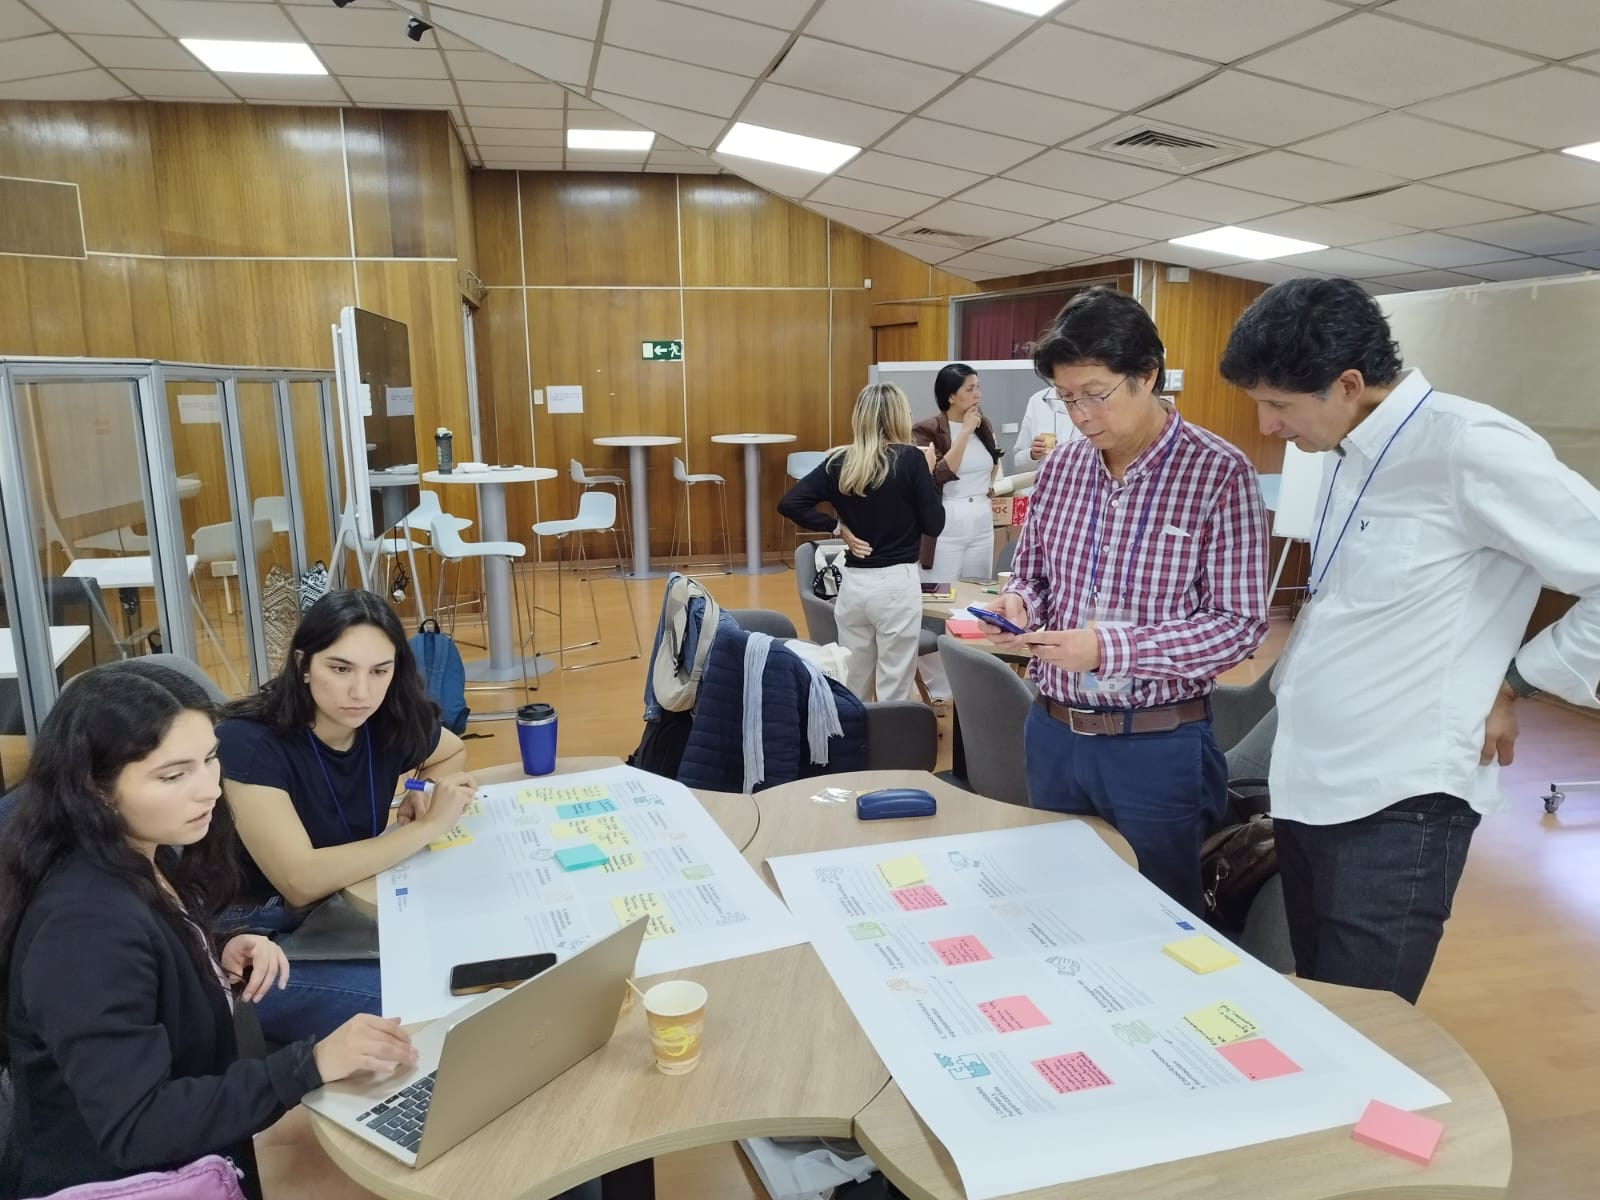
\includegraphics[width=0.6\linewidth,height=\textheight,keepaspectratio]{figures/2.1/Canva-01.jpg}

}

\subcaption{\label{fig-canva2}Workshop developed by each HEIs}

\end{minipage}%
%
\begin{minipage}[t]{0.03\linewidth}
~\end{minipage}%
%
\begin{minipage}[t]{0.48\linewidth}

\centering{

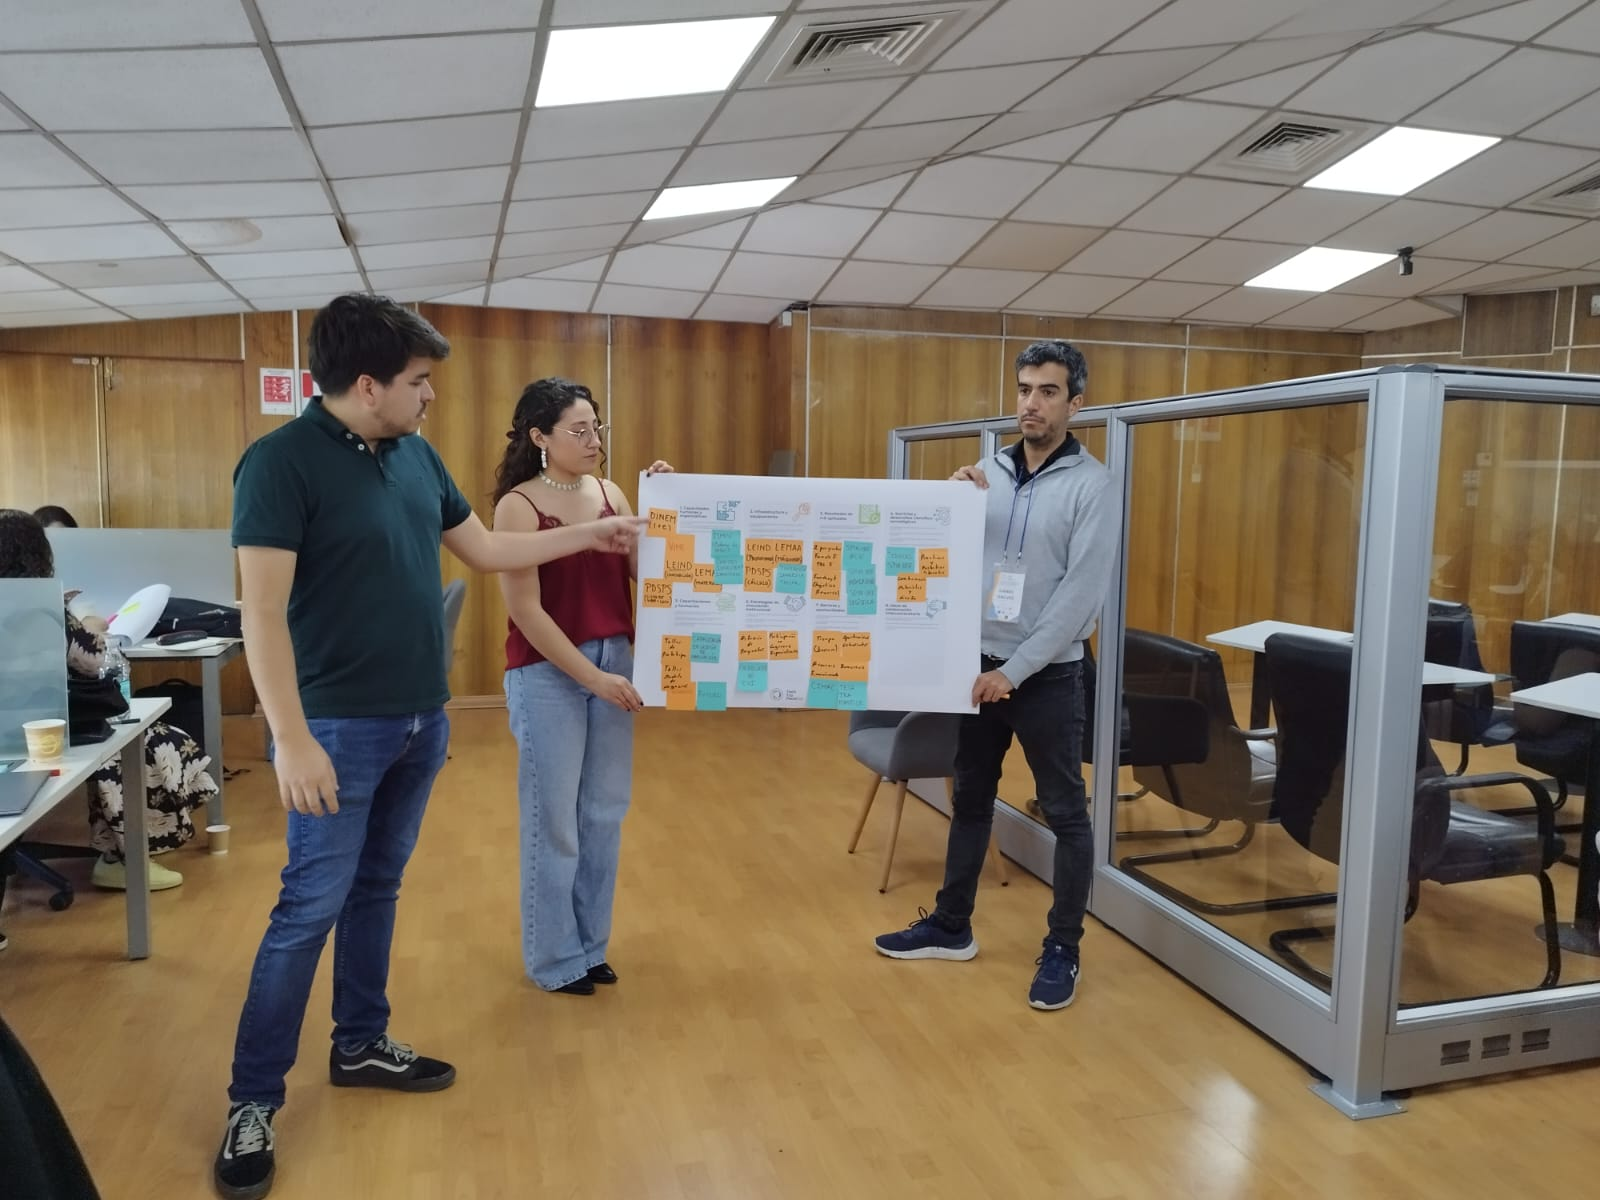
\includegraphics[width=0.6\linewidth,height=\textheight,keepaspectratio]{figures/2.1/Canva-02.jpg}

}

\subcaption{\label{fig-canva3}Feedback made by the consortium meeting at
Chile in Nov.~2025}

\end{minipage}%

\caption{\label{fig-workshop}Socialization of the canva for each HEI}

\end{figure}%

Together, these sources constitute a comprehensive and multi-layered
dataset that will be fully used during the WP2 development, enabling
both systematic analysis and contextual interpretation of the technology
transfer capacities within the consortium.

\section{Key performance indicators}\label{key-performance-indicators}

Table~\ref{tbl-kpi} presents the key performance indicators defined to
assess the implementation and effectiveness of Task 2.1. These
indicators provide a quantitative overview of the data collection
process and the scope of the information gathered across partner
institutions. Results demonstrate a high level of engagement and
consistency among the participating universities. Responses of the four
structured questionnaires reached 100\% of the member universities, all
of which completed the process. This full participation ensured a
comprehensive dataset, enabling a robust characterization of technology
transfer capacities within the consortium.

In terms of raw data content, the collection process resulted in the
identification of 127 services, 83 capacities, 44 training offers, and
49 developments. These reflect the diversity and breadth of activities
carried out by the partner institutions in the field of plastic circular
economy. Moreover, it is important to note that each entry corresponds
to an individual form submitted by the partners, without prior
aggregation or normalization. This approach preserves the granularity of
the information. More detailed and accurate analysis is presented in the
following deliverables.

\begin{table}[H]

\caption{\label{tbl-kpi}Key performance indicators of Task 2.1.}

\centering{

\centering\begingroup\fontsize{11}{13}\selectfont

\begin{tabular}[t]{>{\raggedright\arraybackslash}p{8cm}>{\raggedright\arraybackslash}p{3cm}}
\toprule
\begingroup\fontsize{12}{14}\selectfont \cellcolor{Naranja}{\textcolor{white}{\textbf{Description}}}\endgroup & \begingroup\fontsize{12}{14}\selectfont \cellcolor{Naranja}{\textcolor{white}{\textbf{Value}}}\endgroup\\
\midrule
Number of questionnaires developed & 4\\
\midrule\addlinespace
Number of partners provided with questionnaires & 100\% of the member universities\\
\midrule\addlinespace
Completion rate of questionnaires & 100\%\\
\midrule\addlinespace
Number of services identified* & 127\\
\midrule\addlinespace
Number of capacities mapped* & 83\\
\midrule\addlinespace
Number of training offers* & 44\\
\midrule\addlinespace
Number of developments* & 49\\
\midrule\addlinespace
\begingroup\fontsize{8}{10}\selectfont *Each entry corresponds to one individual form submitted by partners, without prior aggregation or normalization.\endgroup & \begingroup\fontsize{8}{10}\selectfont \endgroup\\
\bottomrule
\end{tabular}
\endgroup{}

}

\end{table}%

\chapter{Conclusions}\label{conclusions}

D2.1 establishes the baseline mapping of institutional services,
capacities, developments, and training activities across the
TechTraPlastiCE consortium. This mapping provides a structured overview
of the existing competencies within partner institutions and their
potential contribution to the circular economy of plastics.

The use of structured questionnaires, combined with an iterative data
collection process and an interactive, canvas-based co-creation
workshop, enabled the systematic collection of both standardized and
context-specific information. This approach ensured comparability across
partners while capturing the diversity of institutional profiles and
Regional contexts.

The results reflect a broad range of institutional strengths, including
technical services, research and innovation capabilities, applied
developments with transfer potential, and training activities oriented
toward socio-economic actors. These elements constitute the foundational
components for the development of institutional portfolios and the
strengthening of university--industry collaboration within the project.

At the same time, the dataset highlights variability in the level of
detail, terminology, and structure across partner contributions. While
this reflects the diversity of institutional contexts, it also indicates
the need for further harmonization and analytical processing.

In this context, the present deliverable is limited to the structured
collection and organization of raw data, ensuring transparency and
traceability of inputs. The subsequent stages, including data
harmonization, coding, comparative analysis, and identification of
strategic priorities, will be developed in Deliverable D2.2.

Overall, D2.1 provides the empirical foundation for advancing toward the
co-creation of institutional portfolios and the implementation of a
progressive technology transfer approach, supporting the transition from
diagnostic understanding to actionable strategies in the circular
economy of plastics.

\appendix

\chapter{Annexes}\label{annexes}

\section{Questionnaires used in the
WP2}\label{questionnaires-used-in-the-wp2}

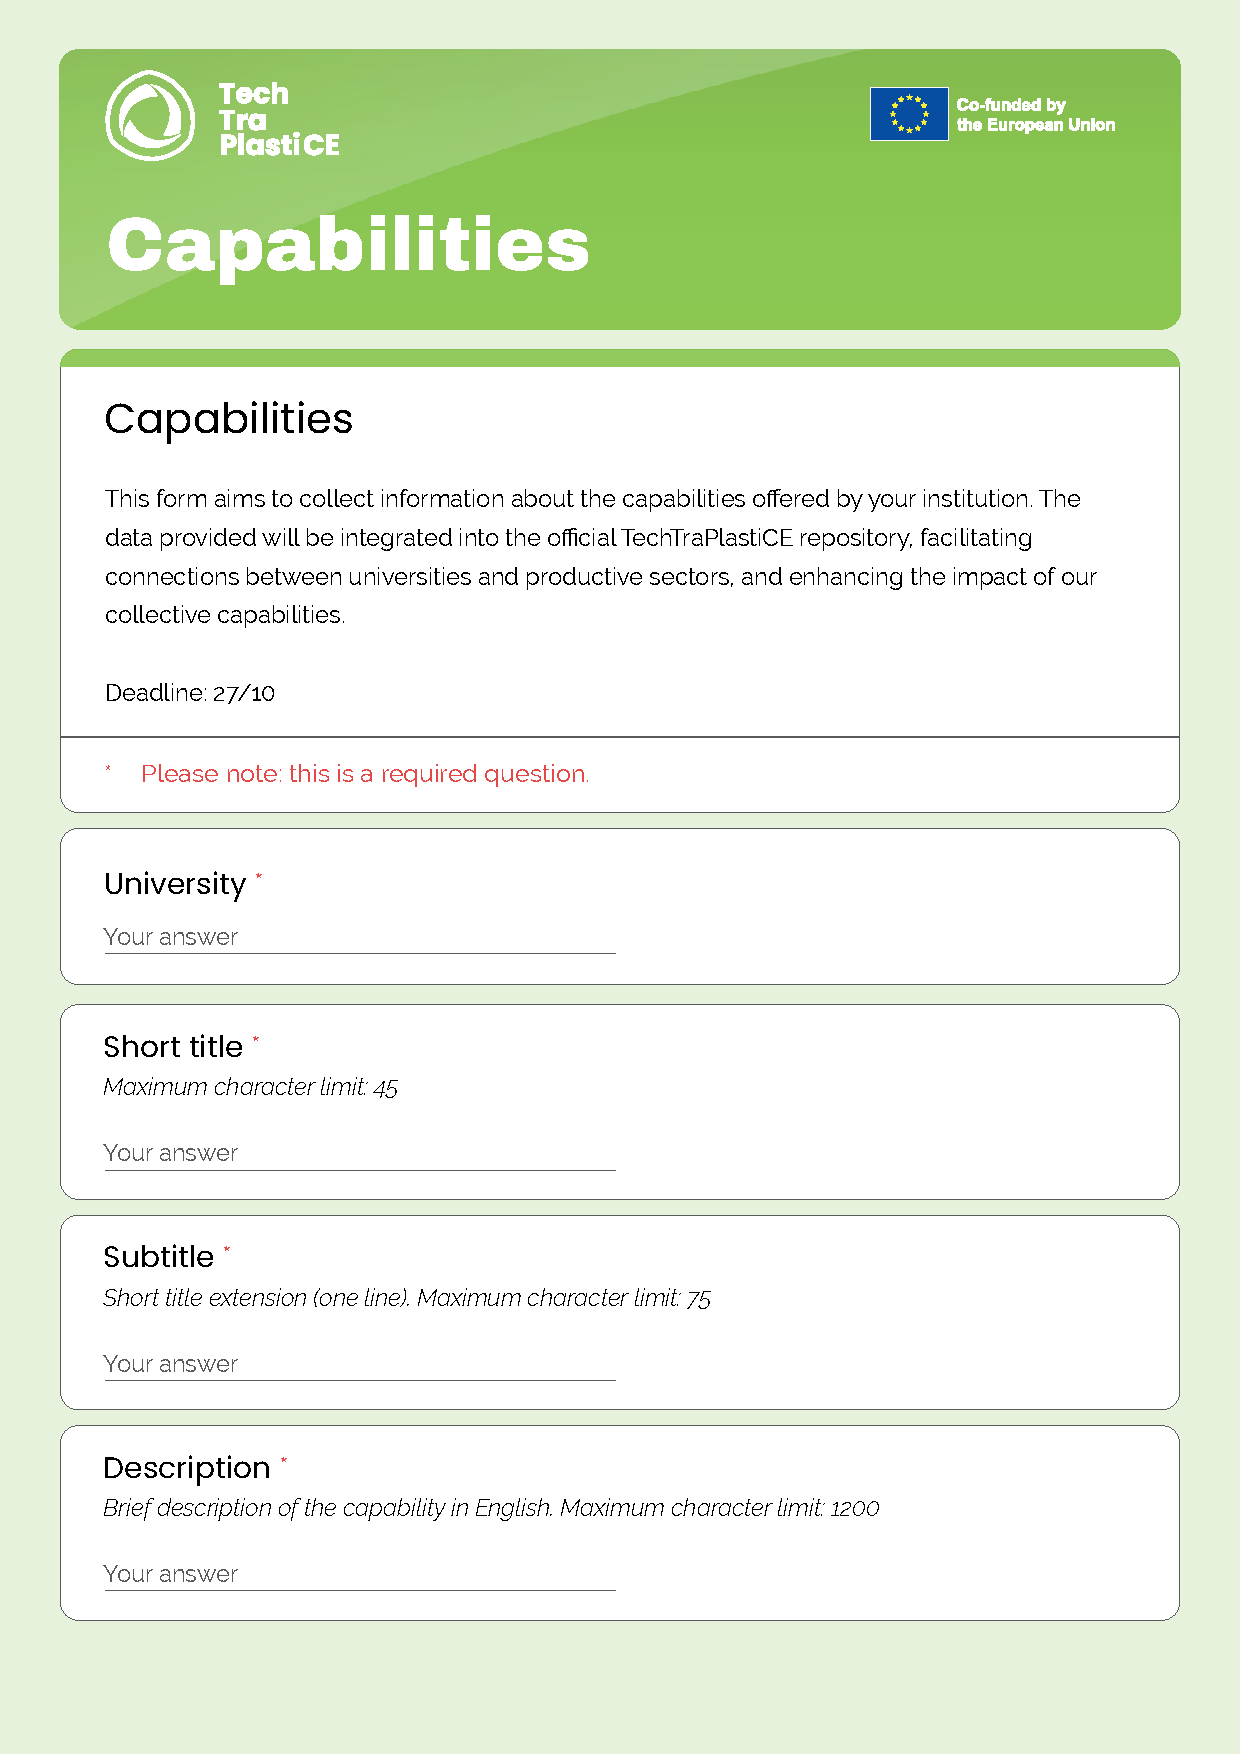
\includepdf[scale=0.77, offset=0 0cm, pagecommand*={\pagestyle{fancy} \subsubsection{ Capabilities }},
pagecommand={\pagestyle{fancy}},
pages=-]{annex/2.1/Annex-Capabilities_a4.pdf}

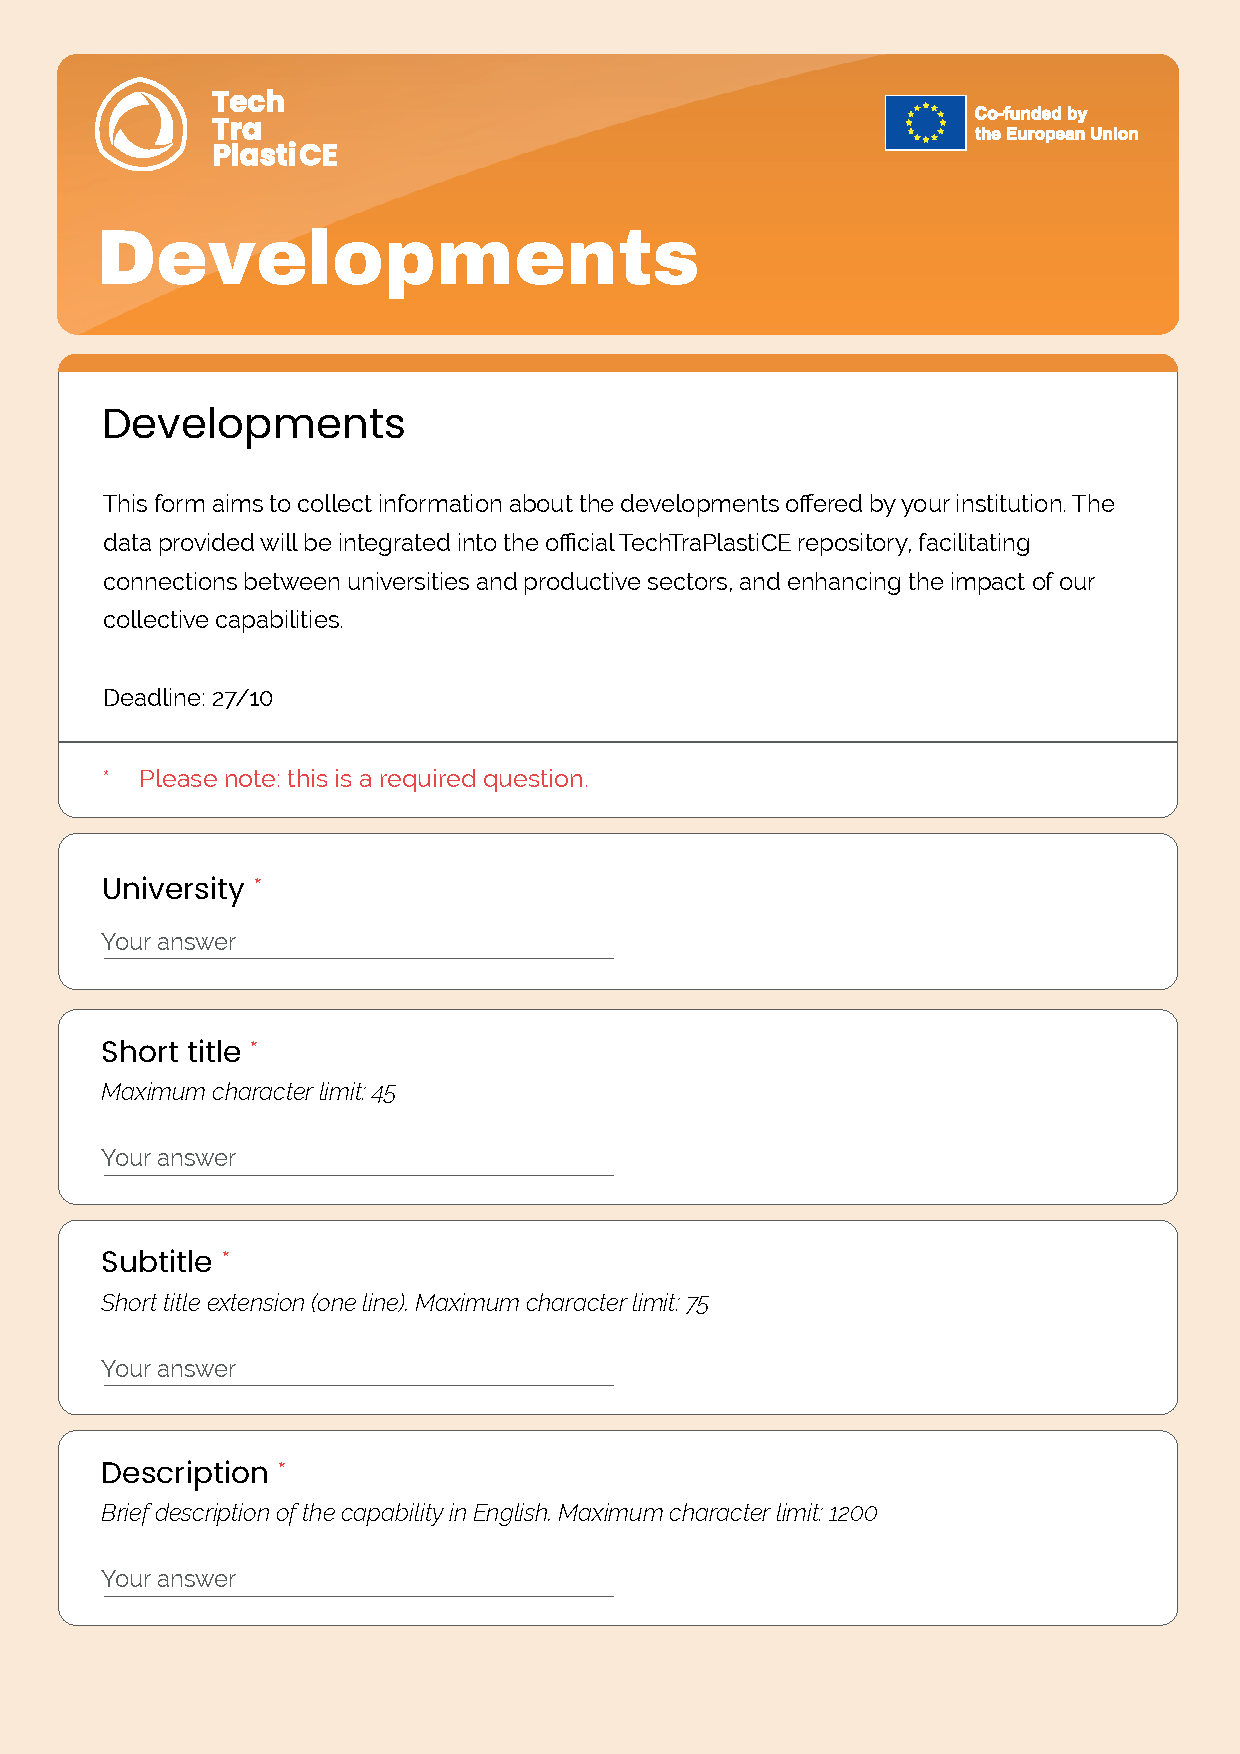
\includepdf[scale=0.77, offset=0 0cm, pagecommand*={\pagestyle{fancy} \subsubsection{Developments}},
pagecommand={\pagestyle{fancy}},
pages=-]{annex/2.1/Annex-developments_a4.pdf}

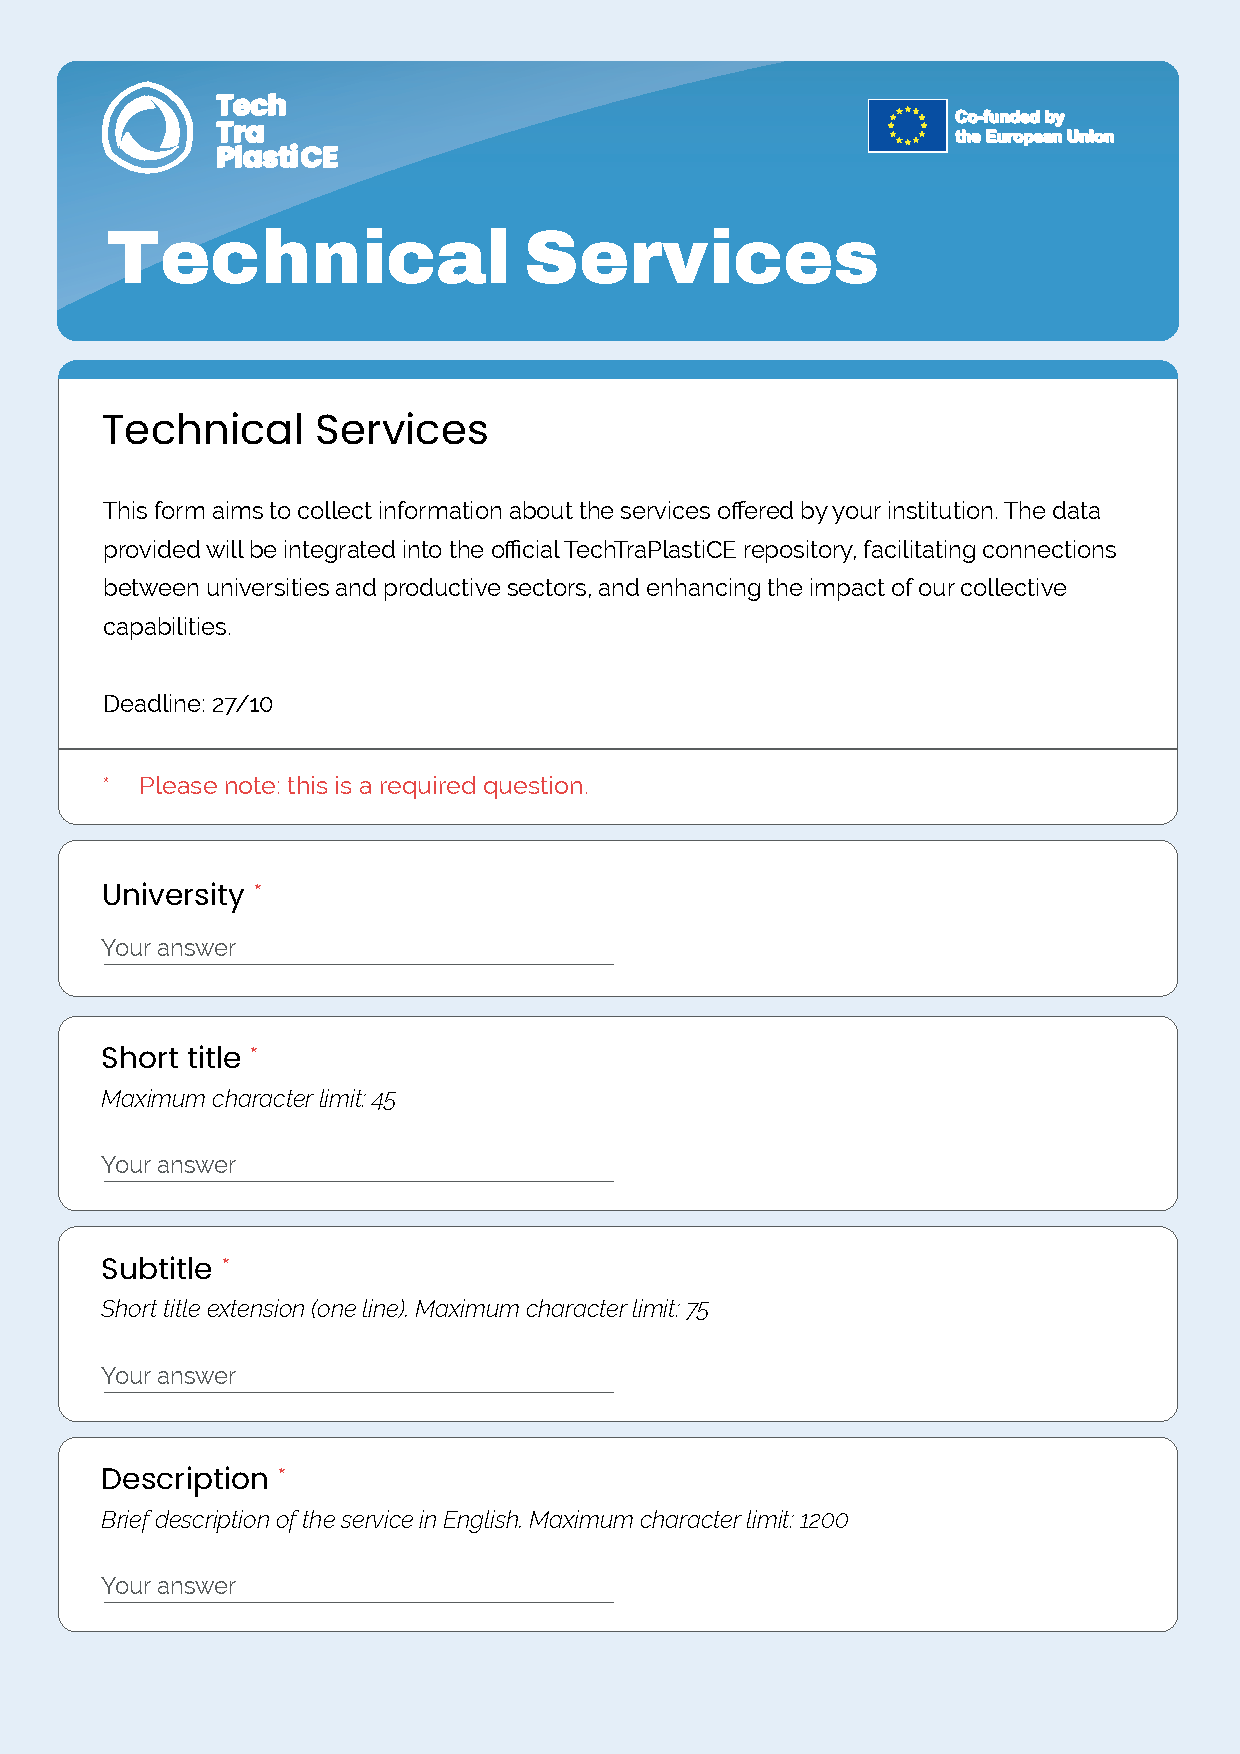
\includepdf[scale=0.77, offset=0 0cm, pagecommand*={\pagestyle{fancy} \subsubsection{Services}},
pagecommand={\pagestyle{fancy}},
pages=-]{annex/2.1/Annex-Services_a4.pdf}

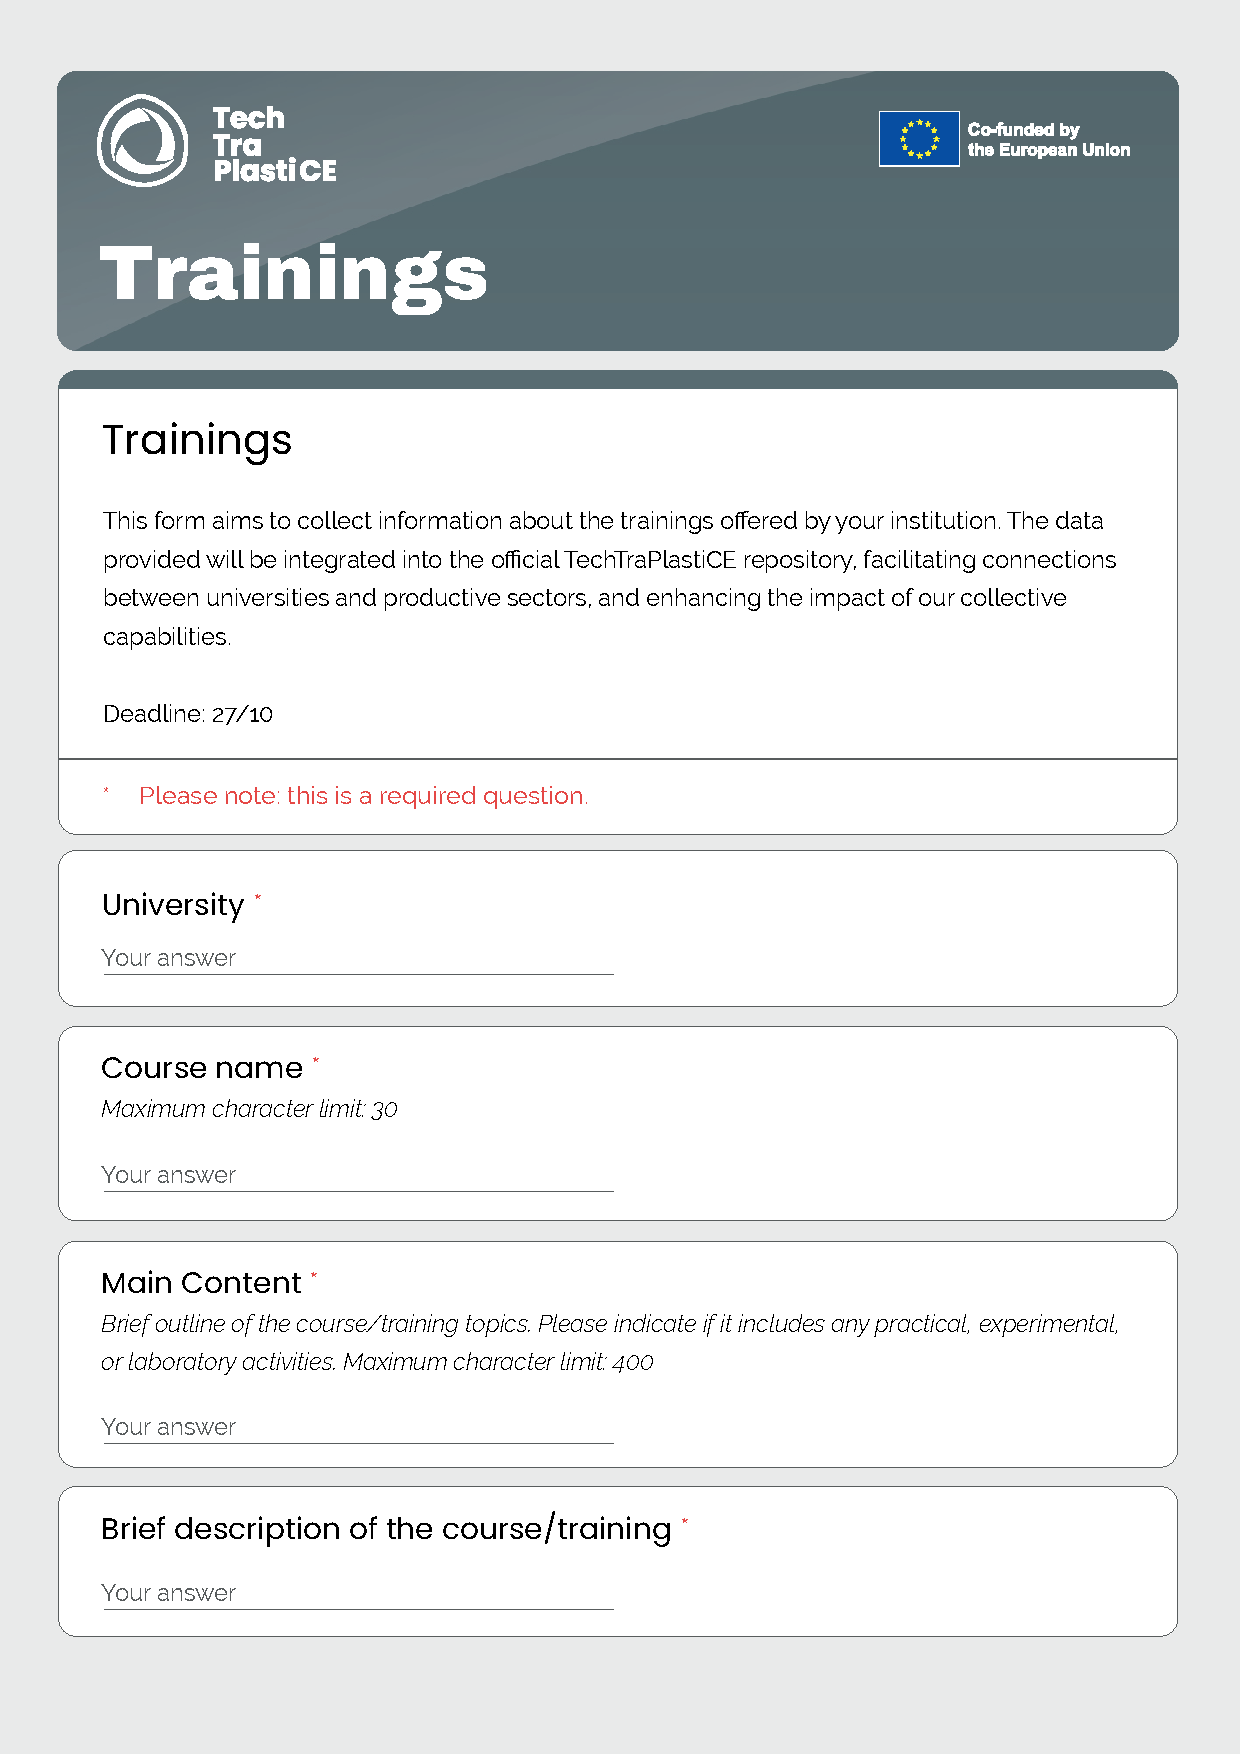
\includepdf[scale=0.77, offset=0 0cm, pagecommand*={\pagestyle{fancy} \subsubsection{Trainings}},
pagecommand={\pagestyle{fancy}},
pages=-]{annex/2.1/Annex-Trainings_a4.pdf}

\chapter{Complete raw data collected throughout T2.1}\label{sec-A2}

\section{Complete collected data -
Developments}\label{complete-collected-data---developments}

\newgeometry{a1paper , left=15mm,right=15mm, top=20mm, bottom=20mm}

\setlength{\tabcolsep}{2pt}
\renewcommand{\arraystretch}{0.75}

\begin{landscape}

\begingroup\fontsize{3}{5}\selectfont

\begin{longtable*}[t]{>{\raggedleft\arraybackslash}p{0.5mm}>{\raggedright\arraybackslash}p{0.5cm}>{\raggedright\arraybackslash}p{0.5cm}>{\raggedright\arraybackslash}p{0.5cm}>{\raggedright\arraybackslash}p{1cm}>{\raggedright\arraybackslash}p{1cm}>{\raggedright\arraybackslash}p{3.5cm}>{\raggedright\arraybackslash}p{3.5cm}>{\raggedright\arraybackslash}p{2.5cm}>{\raggedright\arraybackslash}p{2.5cm}>{\raggedright\arraybackslash}p{1.5cm}>{\raggedright\arraybackslash}p{1.5cm}>{\raggedright\arraybackslash}p{1cm}>{\raggedright\arraybackslash}p{1cm}}
\toprule
\begingroup\fontsize{4}{6}\selectfont \cellcolor{Naranja}{\textcolor{white}{\textbf{ID}}}\endgroup & \begingroup\fontsize{4}{6}\selectfont \cellcolor{Naranja}{\textcolor{white}{\textbf{HEI}}}\endgroup & \begingroup\fontsize{4}{6}\selectfont \cellcolor{Naranja}{\textcolor{white}{\textbf{Title-ES}}}\endgroup & \begingroup\fontsize{4}{6}\selectfont \cellcolor{Naranja}{\textcolor{white}{\textbf{Title-EN}}}\endgroup & \begingroup\fontsize{4}{6}\selectfont \cellcolor{Naranja}{\textcolor{white}{\textbf{Subtitle-ES}}}\endgroup & \begingroup\fontsize{4}{6}\selectfont \cellcolor{Naranja}{\textcolor{white}{\textbf{Subtitle-EN}}}\endgroup & \begingroup\fontsize{4}{6}\selectfont \cellcolor{Naranja}{\textcolor{white}{\textbf{Description-ES}}}\endgroup & \begingroup\fontsize{4}{6}\selectfont \cellcolor{Naranja}{\textcolor{white}{\textbf{Description-EN}}}\endgroup & \begingroup\fontsize{4}{6}\selectfont \cellcolor{Naranja}{\textcolor{white}{\textbf{Impacts-ES}}}\endgroup & \begingroup\fontsize{4}{6}\selectfont \cellcolor{Naranja}{\textcolor{white}{\textbf{Impacts-EN}}}\endgroup & \begingroup\fontsize{4}{6}\selectfont \cellcolor{Naranja}{\textcolor{white}{\textbf{TRL}}}\endgroup & \begingroup\fontsize{4}{6}\selectfont \cellcolor{Naranja}{\textcolor{white}{\textbf{Results}}}\endgroup & \begingroup\fontsize{4}{6}\selectfont \cellcolor{Naranja}{\textcolor{white}{\textbf{Field}}}\endgroup & \begingroup\fontsize{4}{6}\selectfont \cellcolor{Naranja}{\textcolor{white}{\textbf{Keywords}}}\endgroup\\
\midrule
\endfirsthead
\multicolumn{14}{@{}l}{\textit{(continued)}}\\
\toprule
\begingroup\fontsize{4}{6}\selectfont \cellcolor{Naranja}{\textcolor{white}{\textbf{ID}}}\endgroup & \begingroup\fontsize{4}{6}\selectfont \cellcolor{Naranja}{\textcolor{white}{\textbf{HEI}}}\endgroup & \begingroup\fontsize{4}{6}\selectfont \cellcolor{Naranja}{\textcolor{white}{\textbf{Title-ES}}}\endgroup & \begingroup\fontsize{4}{6}\selectfont \cellcolor{Naranja}{\textcolor{white}{\textbf{Title-EN}}}\endgroup & \begingroup\fontsize{4}{6}\selectfont \cellcolor{Naranja}{\textcolor{white}{\textbf{Subtitle-ES}}}\endgroup & \begingroup\fontsize{4}{6}\selectfont \cellcolor{Naranja}{\textcolor{white}{\textbf{Subtitle-EN}}}\endgroup & \begingroup\fontsize{4}{6}\selectfont \cellcolor{Naranja}{\textcolor{white}{\textbf{Description-ES}}}\endgroup & \begingroup\fontsize{4}{6}\selectfont \cellcolor{Naranja}{\textcolor{white}{\textbf{Description-EN}}}\endgroup & \begingroup\fontsize{4}{6}\selectfont \cellcolor{Naranja}{\textcolor{white}{\textbf{Impacts-ES}}}\endgroup & \begingroup\fontsize{4}{6}\selectfont \cellcolor{Naranja}{\textcolor{white}{\textbf{Impacts-EN}}}\endgroup & \begingroup\fontsize{4}{6}\selectfont \cellcolor{Naranja}{\textcolor{white}{\textbf{TRL}}}\endgroup & \begingroup\fontsize{4}{6}\selectfont \cellcolor{Naranja}{\textcolor{white}{\textbf{Results}}}\endgroup & \begingroup\fontsize{4}{6}\selectfont \cellcolor{Naranja}{\textcolor{white}{\textbf{Field}}}\endgroup & \begingroup\fontsize{4}{6}\selectfont \cellcolor{Naranja}{\textcolor{white}{\textbf{Keywords}}}\endgroup\\
\midrule
\endhead

\endfoot
\bottomrule
\endlastfoot
1 & Universidade de Aveiro & Reciclaje sostenible del poliestireno expandido & Sustainable recycling of Expanded Polystyrene & Reciclaje sostenible del poliestireno expandido a partir de embalajes & Sustainable recycling of expanded polystyrene from packaging & Se desarrolló un embalaje de EPS que contiene entre un 60 y un 100\% de material reciclado. Un nuevo proceso de reciclaje permite recuperar EPS posconsumo y posindustrial, preservando sus propiedades clave. El material resultante mantiene la resistencia mecánica, el aislamiento y la estabilidad dimensional requeridas para aplicaciones de embalaje. & It was developed EPS packaging containing 60–100\% recycled material. A new recycling process enables the recovery of post-consumer and post-industrial EPS while preserving key properties. The resulting material maintains the mechanical strength, insulation, and dimensional stability required for packaging applications. & Reduce los residuos de EPS y el envío a vertederos
Disminuye las emisiones de CO₂ y el uso de material virgen
Permite el uso circular de EPS posconsumo y posindustrial
Mantiene la resistencia, el aislamiento y la estabilidad para embalajes & Reduces EPS waste and landfill disposal
Lowers CO₂ emissions and virgin material use
Enables circular use of post-consumer and post-industrial EPS
Maintains strength, insulation, and stability for packaging applications & TRL 6: demonstration in a relevant environment & Publicaciones, Report & Plásticos & Economía circular, reciclaje, embalaje / Circular Economy, Recycling, Packaging\\
\midrule\addlinespace
2 & Universidad de Santiago de Chile & Micro Arquitectura Ambiental & Environmental Micro-Architecture & Componente arquitectónico para fachadas en altura con capacidad de remoción de contaminación atmosférica & Architectural component for high-rise facades with the capacity to remove atmospheric pollution & El proyecto investiga el desarrollo de un componente arquitectónico de micro-arquitectura ambiental destinado a fachadas en altura, capaz de contribuir a la remoción de contaminantes atmosféricos presentes en entornos urbanos. A través del diseño arquitectónico, la selección de materiales y la incorporación de principios de fotocatálisis y ventilación pasiva, se busca generar una solución constructiva que actúe de manera activa sobre la calidad del aire, integrándose a la envolvente del edificio sin afectar su desempeño estructural ni estético. & This project explores the development of an environmental micro-architecture component designed for high-rise building façades, aimed at contributing to the removal of atmospheric pollutants in urban environments. Through architectural design, material selection, and the integration of photocatalytic and passive ventilation principles, the project seeks to generate a constructive solution that actively improves air quality while integrating seamlessly into the building envelope without compromising structural or aesthetic performance. & Mejora de la calidad del aire en zonas urbanas densas; Integración de funciones ambientales en la arquitectura; Innovación en envolventes activas para edificios en altura; Contribución a estrategias de mitigación de contaminación urbana & Improvement of air quality in dense urban areas; Integration of environmental functions into architecture; Innovation in active building envelopes; Contribution to urban pollution mitigation strategies & TRL 4: validation in laboratory & Prototipo & Plásticos, Arquitectura, construcción sustentable, diseño urbano, envolventes de edificios & Micro-arquitectura, contaminación atmosférica, fachadas, fotocatálisis\\
\midrule\addlinespace
3 & Universidad de Santiago de Chile & Arquitectura Plástica & Plastic Architecture & Componente arquitectónico tipo ladrillo a partir de upcycling de plástico reciclado PEAD con funciones ambientales & Brick-type architectural component made from upcycled recycled HDPE plastic with environmental functions & El proyecto desarrolla un componente arquitectónico tipo ladrillo fabricado a partir del upcycling de plástico reciclado PEAD, orientado a aplicaciones constructivas con valor ambiental agregado. Mediante procesos de diseño y manufactura experimental, el componente busca integrar funciones como ventilación, absorción acústica o interacción ambiental, promoviendo el uso de residuos plásticos como recurso constructivo y fomentando modelos de economía circular en la arquitectura. & This project develops a brick-type architectural component manufactured from upcycled recycled HDPE plastic, aimed at construction applications with added environmental value. Through experimental design and manufacturing processes, the component integrates functions such as ventilation, acoustic absorption, or environmental interaction, promoting the use of plastic waste as a construction resource and fostering circular economy models in architecture. & Valorización de residuos plásticos; Reducción de huella ambiental en la construcción; Desarrollo de nuevos sistemas constructivos sostenibles & Valorization of plastic waste; Reduction of environmental footprint in construction; Development of new sustainable building systems & TRL 4: validation in laboratory & Prototipo & Plásticos, Construcción, arquitectura & Upcycling, PEAD, ladrillo plástico, arquitectura sustentable\\
\midrule\addlinespace
4 & Universidad de Santiago de Chile & Revestimiento Fotocatalítico PEAD & Photocatalytic HDPE Cladding & Revestimiento tipo listón a partir de PEAD reciclado para degradación de gases contaminantes & Slat-type cladding made from recycled HDPE for degradation of atmospheric pollutants & El proyecto desarrolla un revestimiento arquitectónico tipo listón fabricado con polietileno de alta densidad reciclado (PEAD), incorporando propiedades fotocatalíticas para la degradación de gases contaminantes atmosféricos en entornos urbanos. La investigación combina diseño arquitectónico, ingeniería de materiales y validación ambiental, con el objetivo de generar una solución constructiva activa que contribuya a la descontaminación del aire y al uso avanzado de plásticos reciclados en arquitectura. & This project develops a slat-type architectural cladding manufactured from recycled high-density polyethylene (HDPE), incorporating photocatalytic properties for the degradation of atmospheric pollutant gases in urban environments. The research combines architectural design, materials engineering, and environmental validation to generate an active construction solution that contributes to air decontamination and advanced use of recycled plastics in architecture. & Reducción de contaminantes atmosféricos urbanos; Innovación en revestimientos arquitectónicos activos; Uso avanzado de plásticos reciclados; Impacto positivo en salud urbana & Reduction of urban air pollutants; Innovation in active architectural cladding systems; Advanced use of recycled plastics; Positive impact on urban health & TRL 4: validation in laboratory & Patente, Prototipo & Plásticos, Arquitectura, construcción urbana & Fotocatálisis, PEAD reciclado, contaminación atmosférica, revestimientos\\
\midrule\addlinespace
5 & Universidad de Santiago de Chile & Panel SUMI & SUMI Panel & Panel acústico manufacturado con residuos plásticos de PEAD & Acoustic panel manufactured from HDPE plastic waste & El proyecto “SUMI” desarrolla un panel acústico diseñado y manufacturado a partir de residuos plásticos de PEAD, orientado a aplicaciones en espacios interiores. El enfoque combina diseño, materialidad y desempeño acústico, buscando transformar residuos plásticos en un producto funcional, estético y sustentable, contribuyendo tanto al control acústico como a la valorización creativa de desechos industriales. & The “SUMI” project develops an acoustic panel designed and manufactured from HDPE plastic waste, aimed at interior space applications. The approach combines design, materiality, and acoustic performance, transforming plastic waste into a functional, aesthetic, and sustainable product that contributes to both sound control and creative waste valorization. & Mejora del confort acústico interior; Reutilización de residuos plásticos; Diseño sustentable aplicado & Improvement of indoor acoustic comfort; Reuse of plastic waste; Applied sustainable design & TRL 4: validation in laboratory & Prototipo & Plásticos, Diseño interior, acústica arquitectónica & Panel acústico, PEAD, diseño sustentable, reciclaje\\
\midrule\addlinespace
6 & Universidad de Santiago de Chile & Resonador Acústico Reciclado & Recycled Plastic Acoustic Resonator & Resonador acústico de plástico reciclado para espacios de trabajo & Recycled plastic acoustic resonator for workspaces & El proyecto desarrolla un resonador acústico fabricado a partir de plástico reciclado, destinado a mejorar el confort acústico en espacios de trabajo. Mediante el diseño paramétrico, la experimentación material y la validación acústica, se busca generar un sistema eficiente, sustentable y adaptable, que contribuya a la calidad ambiental interior y al bienestar de los usuarios en contextos laborales. & This project develops an acoustic resonator made from recycled plastic, aimed at improving acoustic comfort in workspaces. Through parametric design, material experimentation, and acoustic validation, the project seeks to create an efficient, sustainable, and adaptable system that enhances indoor environmental quality and user well-being in workplace settings. & Mejora del confort acústico laboral; Aplicación de reciclaje en productos de alto desempeño; Bienestar y productividad en espacios de trabajo & Improvement of workplace acoustic comfort; Application of recycling in high-performance products; Enhanced well-being and productivity & TRL 4: validation in laboratory & Prototipo & Plásticos, Salud, Arquitectura interior, espacios de trabajo, acústica & Resonador acústico, plástico reciclado, confort acústico, diseño sustentable\\
\midrule\addlinespace
7 & Universidad de Santiago de Chile & Juan Fernández Circular & Juan Fernández Circular & Prototipado de productos útiles con plástico reciclado para la comunidad del Archipiélago Juan Fernández & Prototyping useful products from recycled plastics for the Juan Fernández Archipelago community & Iniciativa de I+D donde la USACH, a través del laboratorio LEMAA, participa en el proyecto “Juan Fernández Circular”, impulsado por CircularTec y financiado por ANID, para abordar la acumulación de residuos plásticos en el archipiélago mediante economía circular. En una primera etapa se realizó levantamiento territorial para identificar tipos/cantidades de plásticos y objetos de interés; luego LEMAA caracterizó los plásticos más comunes y definió al polipropileno como material apto, desarrollando prototipos de productos (incluyendo señuelos de pesca y abrazaderas) para uso local. & An R\&D initiative in which USACH, through the LEMAA lab, takes part in the “Juan Fernández Circular” project promoted by CircularTec and funded by ANID, addressing plastic waste accumulation in the archipelago through a circular-economy approach. In a first phase, a territorial survey identified plastic types/volumes and locally relevant product needs; then LEMAA characterized common plastics, identified polypropylene as a suitable material, and developed product prototypes (including fishing lures and clamps) for local use & Valorización in situ de residuos plásticos del archipiélago mediante economía circular; Generación de productos útiles para la comunidad local a partir de reciclaje. & In-situ valorization of archipelago plastic waste through circular economy practices; Creation of useful products for the local community from recycled plastics & TRL 5: validation in a relevant environment & Prototipo & Plásticos & Economía circular, reciclaje, polipropileno,Juan Fernández\\
\midrule\addlinespace
8 & Universidad de Santiago de Chile & PALF: Palmeta Fotovoltaica Modular & PALF: Modular Photovoltaic Tile & Sistema de iluminación autosuficiente con plástico reciclado y energía solar para zonas críticas del campus & Self-sufficient lighting system using recycled plastic and solar energy for critical campus areas & PALF es un sistema modular de iluminación autosuficiente creado por el equipo LEMAA para mejorar visibilidad y seguridad en sectores críticos del campus USACH. Usa celdas fotovoltaicas sobre bases de plástico reciclado, no requiere red eléctrica ni obras invasivas y es escalable. Ganó el primer lugar en “Luz Verde” USACH Sostenible y cuenta con un piloto con dos luminarias solares de 8.000 lúmenes. & PALF is a modular, self-sufficient lighting system developed by the LEMAA team to improve visibility and perceived safety in critical areas of the USACH campus. It uses photovoltaic cells mounted on recycled plastic bases, requires no grid connection or invasive works, and is scalable. It won first place in the “Luz Verde” category of USACH Sostenible and has a pilot with two 8,000-lumen solar luminaires. & Mejora de iluminación, seguridad y experiencia de la comunidad universitaria; Solución replicable y modular sin estructuras adicionales ni conexión a red; Uso de polímeros reciclados y energía renovable (baja huella). & Improved lighting, safety, and user experience for the university community; Replicable modular solution without extra structures or grid connection; Use of recycled polymers and renewable energy (lower footprint). & TRL 4: validation in laboratory & Prototipo & Plásticos, Iluminación urbana/campus, energía solar, & Iluminación solar, fotovoltaico, modular, plástico reciclado\\
\midrule\addlinespace
9 & Universidad de Santiago de Chile & Planta virtual de reciclaje para economía circular & Virtual recycling plant for circular economy learning & Experiencia interactiva para la comprensión de procesos de reciclaje y economía circular & Interactive experience for understanding recycling processes and circular economy & Proyecto de innovación docente desarrollado por el LEIND que consiste en una herramienta virtual interactiva que simula el funcionamiento de una planta de reciclaje. Permite a estudiantes experimentar procesos productivos circulares de forma inmersiva, facilitando la comprensión de flujos de materiales, toma de decisiones y principios de economía circular sin necesidad de infraestructura física & Teaching innovation project developed by LEIND consisting of an interactive virtual tool that simulates a recycling plant. It allows students to experience circular production processes immersively, supporting the understanding of material flows, decision-making and circular economy principles without physical infrastructure & Mejora del aprendizaje experiencial en economía circular; Reducción de barreras de acceso a infraestructura industrial; Fortalecimiento de competencias en sostenibilidad e innovación & Enhanced experiential learning in circular economy; Reduced barriers to access industrial infrastructure; Strengthened sustainability and innovation skills & TRL 4: validation in laboratory & Publicaciones, Prototipo & Educación Superior & RV, reciclaje, aprendizaje / VR, recycling, learning\\
\midrule\addlinespace
10 & Universidad de Santiago de Chile & Ayudantes virtuales con IA para innovación & AI virtual teaching assistants for innovation courses & Apoyo inteligente al aprendizaje en creatividad e innovación & Intelligent support for learning creativity and innovation & Desarrollo orientado a la implementación de asistentes virtuales basados en inteligencia artificial como apoyo al proceso de aprendizaje en Ingeniería Industrial, con foco en curso en cursos de creatividad e innovación. Estos sistemas facilitan retroalimentación, acompañamiento conceptual y orientación metodológica. & Development focused on implementing AI-based virtual assistants to support learning processes in Industrial Engineering, particularly in creativity and innovation courses. These systems provide feedback, conceptual support and methodological guidance & Mejora del acompañamiento al estudiante; Escalabilidad del apoyo docente; Aprendizaje personalizado & Improved student support; Scalable teaching assistance; Personalized learning & TRL 4: validation in laboratory & Publicaciones, Prototipo & Educación Superior & Educación, innovación, IA / Education, innovation, AI\\
\midrule\addlinespace
11 & Universidad de Santiago de Chile & Reciclaje local de plástico para impresión 3D & Local plastic recycling for additive manufacturing & Economía circular aplicada a espacios de innovación & Applied circular economy in innovation spaces & Desarrollo de un sistema local de reciclaje de residuos plásticos orientado a su reutilización en procesos de manufactura aditiva. El proyecto integra economía circular, prototipado y aprendizaje práctico en espacios de innovación & Development of a local plastic recycling system aimed at reuse in additive manufacturing processes. The project integrates circular economy, prototyping and hands-on learning in innovation spaces & Reducción de residuos plásticos; Reutilización de materiales en prototipado; Formación práctica en economía circular & Plastic waste reduction; Material reuse in prototyping; Hands-on circular economy training & TRL 4: validation in laboratory & Prototipo & Plásticos & reciclaje, plástico, impresión 3D / recycling, plastic, 3D printing\\
\midrule\addlinespace
12 & Universidad de Santiago de Chile & Gestión de economía circular empresarial & Circular economy management in companies & Integración de circularidad en procesos organizacionales & Integrating circularity into organizational processes & Desarrollo metodológico orientado a apoyar a empresas en la incorporación de principios de economía circular en sus procesos productivos y organizacionales & Methodological development aimed at supporting companies in integrating circular economy principles into their production and organizational processes & Mejora del desempeño ambiental; Optimización de recursos; Alineación con estrategias sostenibles & Improved environmental performance; Resource optimization & TRL 4: validation in laboratory & Publicaciones, Prototipo & Plásticos, Energía & gestión, economía circular / management, circular economy\\
\midrule\addlinespace
13 & Universidad de Santiago de Chile & Metodologías de gestión de proyectos de innovación sostenible & Sustainable innovation project management methodologies & Estructuración y gestión de proyectos innovadores con enfoque ágil y sostenible. & Structuring and managing innovation projects through agile and sustainability-driven approaches & Desarrollo de metodologías para la gestión de proyectos de innovación sostenible que integran enfoques ágiles, diseño centrado en el usuario y criterios de sostenibilidad desde etapas tempranas. Estas metodologías permiten planificar, ejecutar y evaluar proyectos innovadores considerando impacto, viabilidad y escalabilidad & Development of methodologies for managing sustainable innovation projects that integrate agile approaches, user-centered design and sustainability criteria from early stages. These methodologies support planning, execution and evaluation considering impact, feasibility and scalability & Mayor eficiencia en la gestión de proyectos innovadores
Integración temprana de criterios de sostenibilidad
Mejora en la coordinación de equipos multidisciplinarios
Aumento de la tasa de éxito en proyectos de innovación & Increased efficiency in innovation project management
Early integration of sustainability criteria
Improved coordination of multidisciplinary teams
Higher success rates in innovation projects & TRL 2: formulación del concepto tecnológico & Concepto tecnológico & Gestión proyectos & Metodología, innovación, sostenibilidad / Methodology, innovation, sustainability\\
\midrule\addlinespace
14 & Universidad de Santiago de Chile & Diseño sostenible de cadenas de suministro de recursos de uso común & Sustainable design of common pool resource supply chains & Enfoques de diseño y modelación para la gestión sostenible de recursos compartidos & Design and modeling approaches for the sustainable management of shared resources & Proyecto de investigación FONDECYT orientado al análisis y diseño de cadenas de suministro asociadas a recursos de uso común (common pool resources), integrando criterios de sostenibilidad, eficiencia y gobernanza. El estudio aborda la complejidad de estos sistemas mediante enfoques analíticos y de modelación, considerando interacciones entre actores, restricciones ambientales y dinámicas productivas & FONDECYT research project focused on the analysis and design of supply chains associated with common pool resources, integrating sustainability, efficiency and governance criteria. The project addresses system complexity through analytical and modeling approaches, considering stakeholder interactions, environmental constraints and productive dynamics & Mejora en el diseño y gestión sostenible de cadenas de suministro; Aporte a políticas públicas relacionadas con recursos compartidos; Reducción de impactos ambientales en sistemas productivos; Generación de conocimiento aplicado en sostenibilidad y logística & Improved sustainable design and management of supply chains; Contribution to public policies related to shared resources; Reduction of environmental impacts in production systems; Generation of applied knowledge in sustainability and logistics & TRL 3: experimental proof of concept & Prototipo & Plásticos, Energía, Cadenas de suministro & Sostenible, diseño, recursos / Sustainable, design, resources\\
\midrule\addlinespace
15 & Universidad de Santiago de Chile & Gestión de la innovación sostenible & Sustainable innovation management & Integración estratégica de sostenibilidad, innovación y creación de valor en organizaciones y emprendimiento & Strategic integration of sustainability, innovation and value creation in organizations and startups & Desarrollo metodológico orientado a apoyar organizaciones, emprendimientos y proyectos en la incorporación sistemática de la sostenibilidad dentro de sus procesos de innovación. El enfoque combina herramientas de gestión de la innovación, sostenibilidad y economía circular, permitiendo diseñar, evaluar y escalar iniciativas innovadoras alineadas con criterios ambientales, sociales y económicos & Methodological development aimed at supporting organizations, startups and projects in the systematic integration of sustainability into innovation processes. The approach combines innovation management, sustainability and circular economy tools to design, assess and scale initiatives aligned with environmental, social and economic criteria & Mejora en la toma de decisiones estratégicas con enfoque sostenible
Reducción de riesgos ambientales y reputacionales
Aumento del valor social y económico de proyectos innovadores
Fortalecimiento de capacidades organizacionales en innovación sostenible & Improved strategic decision-making with a sustainability focus
Reduction of environmental and reputational risks
Increased social and economic value of innovation projects
Strengthened organizational capabilities in sustainable innovation & TRL 2: formulación del concepto tecnológico & Formulación del concepto & Innovación Sostenible & gestión, estrategia, sostenibilidad / management, strategy, sustainability\\
\midrule\addlinespace
16 & Universidad Nacional del Sur & Reciclado de plásticos RAEE & Plastics WEEE recycling & Agregado de valor de plásticos provenientes de artículos de eléctrica y electrónica & Value added of plastic from waste electrical and electronic equipment & Desarrollo de estrategias específicas para el reciclado de mezclas de Poliestireno de Alto Impacto (HIPS)/Acrilonitrilo Butadieno Estireno (ABS) provenientes de RAEE con y sin compatibilización involucrada. Incremento del valor agregado por la mejora de las propiedades finales de las mezclas. Estas pueden reemplazar directamente el HIPS y el ABS utilizados en equipamiento electrónico. & Tailored recycling strategies for blends of High Impact Polystyrene (HIPS)/Acrylonitrile Butadiene Styrene (ABS) from WEEE with and without compatibilization. Added value by mechanical performance improvement. This recycled material can directly replace starting HIPS or ABS used in electronic equipment. & - Evita la disposición final de plásticos RAEE
- Evita la separación por tipo de plástico
- Reducción de los costos de mano de obra
- Minimización de los residuos plásticos
- Mejora en las ganancias de los recicladores
- Adaptable a sistemas de reciclado tradicionales & - Avoids final disposal of WEEE plastics
- Avoids plastic-type separation
- Reduces labor costs
- Minimizes plastic waste
- Increases recyclers’ profits
- Adaptable to traditional recycling systems & TRL 5: validation in a relevant environment & Además de publicaciones en revistas de alto impacto, actualmente se está trabajando en el desarrollo de productos específicos fabricados a partir de las estrategias validadas. & Plásticos & SOSTENIBILIDAD DE PLÁSTICOS, RECICLADO, RAEE / PLASTIC SUSTAINABILITY, RECYCLING, WEEE\\
\midrule\addlinespace
17 & Universidad Nacional del Sur & Sensores para Envases Inteligentes & Sensors for Smart Packaging & PELÍCULAS FLEXIBLES CON GRAFENO PARA DETECCIÓN DE BACTERIAS EN CARNE & FLEXIBLE GRAPHENE-BASED FILMS FOR BACTERIAL DETECTION IN MEAT & Desarrollo de sensores basados en películas poliméricas recubiertas
con grafeno para la detección in situ de Escherichia coli en carnes y
productos cárnicos. Se evalúan su sensibilidad, límite de detección,
estabilidad y compatibilidad con envases flexibles, considerando
requisitos de seguridad alimentaria y viabilidad tecnológica para su
implementación industrial. & Development of sensors based on graphene-coated polymeric films
for the in situ detection of Escherichia coli in meat and meat
products. Sensitivity, limit of detection, stability, and compatibility
with flexible packaging are evaluated, considering food safety
requirements and technological feasibility for industrial
implementation. & Detección temprana de patógenos.
Reducción de riesgos sanitarios y pérdidas económicas.
Innovación en envases plásticos. & Early pathogen detection.
Reduction of health risks and economic losses.
Innovation in plastic packaging. & TRL 4: validation in laboratory & Publicaciones, validación en laboratorio & Plásticos, Alimentos, Sensores eléctricos & SENSORES, ENVASES INTELIGENTES, ESCHERICHIA COLI; SENSORS, SMART PACKAGING, ESCHERICHIA COLI\\
\midrule\addlinespace
18 & Universidad Nacional del Sur & Envases Multicapa Mono-material & Multilayer Mono-material Packaging & ENVASES COMPUESTOS MULTICAPA BASADOS EN POLIOLEFINAS CON PROPIEDADES A MEDIDA & MULTILAYER POLYOLEFIN-BASED COMPOSITE PACKAGING WITH TAILORED PROPERTIES & Desarrollo de películas multicapa mono-material de base
polipropileno con capas cargadas con talco y caolín. Las películas
obtenidas mejoran la barrera a la luz UV y visible, aumentan rigidez
y estabilidad térmica, y mantienen las propiedades mecánicas y de
barrera a gases. Diseñadas como una alternativa reciclable a los
envases multi-material para productos fotosensibles. & Development of mono-material multilayer polypropylene films
incorporating talc- and kaolinite-filled layers. The resulting films
improve UV and visible light barrier performance, increase stiffness
and thermal stability, while maintaining mechanical strength and gas
barrier properties. Designed as a recyclable alternative to
conventional multi-material packaging for photosensitive products. & Compatible con tecnologías convencionales de procesamiento de
poliolefinas
Facilita el reciclado mecánico al eliminar estructuras multi-material.
Reduce la generación de residuos mediante el diseño orientado a la
reciclabilidad.
Contribuye a estrategias de economía circular en cadenas de valor
de poliolefinas. & Compatible with conventional polyolefin processing technologies.
Facilitates mechanical recycling by eliminating multi-material
structures.
Reduces waste generation through design for recyclability.
Supports circular economy strategies within polyolefin value chains. & TRL 4: validation in laboratory & Publicaciones, validación en laboratorio & Plásticos, Alimentos, Productos fotosensibles & PELÍCULAS MONOMATERIAL MULTICAPA, ECODISEÑO, PROPIEDADES BARRERA; MONO-MATERIAL MULTILAYER FILMS, RECYCLABLE, LIGHT BARRIER PROPERTIES\\
\midrule\addlinespace
19 & Universidad Nacional del Sur & Películas de Almidón & Starch Films & PELÍCULAS DE ALMIDÓN CON FUNCIONALIDADES ESPECÍFICAS & STARCH FILMS WITH SPECIFIC FUNCTIONALITIES & Las películas de almidón son consideradas potenciales sustitutos de
los plásticos convencionales en muchas aplicaciones industriales,
siguiendo la tendencia mundial de la preservación del
medioambiente. Esta tecnología permite producir películas de
almidón conteniendo rellenos o compuestos activos que incrementa
la performance del producto. & Starch films are considered potential substitutes for conventional
plastics in many industrial applications, following global trends of
environmental preservation. This technology allows to produce
starch films containing fillers or active compounds that increase the
product performance. & Biodegradable
Obtenido a partir de materias primas renovables
Inocuo y biocompatible
Permeabilidad selectiva a los gases
Películas de almidón diseñadas por mezclado con rellenos y otros
polímeros & Biodegradable
Obtained from a renewable raw material
Innocuous and biocompatible
Selective gases permeability & TRL 6: demonstration in a relevant environment & Publicaciones, demostración en entorno relevante & Plásticos, Alimentos, Recubrimientos biopoliméricos & MATERIALES BIODEGRADABLES, PELÍCULAS DE ALMIDÓN, ENVASES SOSTENIBLES; BIODEGRADABLE PACKAGING MATERIALS, BIO-BASED FILMS, SUSTAINABLE FOOD PACKAGING\\
\midrule\addlinespace
20 & Universidad Nacional del Sur & Mezclas de Polímeros & Polymer Blends & DESARROLLO A MEDIDA DE MEZCLAS TERMOPLÁSTICAS PARA EXTRUSIÓN, MOLDEO POR INYECCIÓN Y SOPLADO & EXTRUSION, INJECTION AND BLOW MOLDING OF TAILORED THERMOPLASTIC BLENDS & Desarrollo de mezclas poliméricas con propiedades mecánicas y de
flujo específicas, incluyendo el uso de termoplásticos, elastómeros,
cargas orgánicas e inorgánicas y polímeros biodegradables. & Development of polymeric blends with specific mechanical and flow
properties, involving the use of thermoplastics, elastomers, organic
and inorganic fillers and biodegradable polymers. & Las mezclas pueden ajustarse para satisfacer los requerimientos de
los productos finales. & Blends may be tailored to suit specific needs of final products. & TRL 9: system validated in operational environment & Publicaciones, sistema probado y operativo en un entorno real & Plásticos, Mezclas poliméricas para mezclado reactivo, extrusión, moldeo por inyección y soplado & MEZCLAS POLIMÉRICAS, EXTRUSIÓN E INYECCIÓN, CARGAS; CUSTOMIZED POLYMER FORMULATIONS, TAILOR-MADE THERMOPLASTIC COMPOUNDS, EXTRUSION, INJECTION AND BLOW MOLDING\\
\midrule\addlinespace
21 & Universidad Nacional del Sur & Polihidroxialcanoatos PHAs & Polyhydroxyalkanoates PHAs & BIOSÍNTESIS DE POLIHIDROXIALCANOATOS Y COPOLÍMEROS & BIOSYNTHESIS OF POLYHYDROXYALKANOATES AND COPOLYMERS & Los PHAs son poliésteres termoplásticos producidos por muchos
microorganismos como fuentes de carbono y energía. Pueden
obtenerse diferentes copolímeros empleando cepas autóctonas y
diversas fuentes de carbono de bajo costo (almidón, glicerol y
residuos lignocelulósicos, entre otras). & PHAs are thermoplastic polyesters produced as carbon and energy
sources by several microorganisms. Different copolymers are
obtained by using autochthonous strains and several low-cost
carbon sources (starch, glycerol, lignocellulosic residues, among
others). & Bajo costo de producción usando cepas autóctonas y fuentes de
carbono económicas
Polímeros termoplásticos biodegradables con buen desempeño
mecánico & Low-cost production by using autochthonous strains and cheap
carbon sources
Biodegradable thermoplastic polymers with good mechanical
performance & TRL 4: validation in laboratory & Publicaciones, validación a escala laboratorio & Plásticos, Alimentos, Insumos biomédicos; Productos farmacéuticos & BIOSÍNTESIS DE BIOPOLÍMEROS, PHA, PRODUCCIÓN MICROBIANA DE POLÍMEROS; BIOPOLYMER BIOSYNTHESIS, BIODEGRADABLE THERMOPLASTICS, MICROBIAL POLYMER PRODUCTION\\
\midrule\addlinespace
22 & Universidad Nacional del Sur & Reciclado de Plásticos RAEE & Plastic WEEE Recycling & VALOR AGREGADO A RESIDUOS PLÁSTICOS DE ARTÍCULOS DE ELÉCTRICA Y ELECTRÓNICA & ADDED VALUE TO PLASTIC WASTE FROM ELECTRICAL AND ELECTRONIC EQUIPMENT & Desarrollo de estrategias específicas para el reciclado de mezclas
de Poliestireno de Alto Impacto (HIPS)/Acrilonitrilo Butadieno
Estireno (ABS) provenientes de RAEE con y sin compatibilización
involucrada. Incremento del valor agregado por la mejora de las
propiedades finales de las mezclas. Estas pueden reemplazar
directamente el HIPS y el ABS utilizados en equipamiento
electrónico. & Tailored recycling strategies for blends of High Impact Polystyrene
(HIPS)/Acrylonitrile Butadiene Styrene (ABS) from WEEE with and
without compatibilization. Added value by mechanical performance
improvement. This recycled material can directly replace starting
HIPS or ABS used in electronic equipment. & Evita la separación por tipo de plástico
Reducción de los costos de mano de obra
Minimización de los residuos plásticos
Mejora en las ganancias de los recicladores
Fácil procesamiento
Beneficios sostenibles & Avoids final disposal of WEEE plastics
Avoids plastic-type separation
Reduces labor costs
Minimizes plastic waste
Increases recyclers’ profits
Adaptable to traditional recycling systems & TRL 5: validation in a relevant environment & Publicaciones, Prototipo, validación en entorno relevante & Plásticos, Carcasas de eléctrica y electrónica; Alumbrado público; Carcasas para ópticas de automóviles & SOSTENIBILIDAD DE PLÁSTICOS, RECICLAJE, RAEE; PLASTIC SUSTAINABILITY, RECYCLING, WEEE\\
\midrule\addlinespace
23 & Universidad Nacional del Sur & Papel Plástico & Plastic Paper & DESARROLLO DE PELÍCULAS DE POLIOLEFINAS, IMPRIMIBLES, ESCRIBIBLES Y PINTABLES & WRITABLE, PRINTABLE AND PAINTABLE POLYOLEFIN PLASTIC FILMS & Este desarrollo le confiere a las películas plásticas propiedades
similares a las del papel celulósico. Esto se logra mediante un
proceso de bajo costo de incorporación de partículas minerales u
orgánicas en la superficie de dichas películas sin uso de adhesivos.
Las películas resultantes pueden ser impresas con impresoras de
chorro de tinta, escritas con lápiz, birome o fibra y pintadas o teñidas
con variedad de pinturas y tintas. & The development confer to plastic films similar properties to the
cellulose paper. The low-cost process, that makes the films
outstanding materials, attaches mineral /organic particles on the film
surface without adhesives. They can be written with pencils, painted
with tempera and inkjet printed. & Reusable y reciclable.
Fácil de borrar y reescribir con lápiz.
Pintable con pinturas base agua.
Combina las propiedades del papel con las del plástico.
Proceso de producción simple, fácil y sustentable. & Reusable and recyclable
Easy to erase and rewrite with pencil
Paintable with water-based paints
Combine paper properties with the plastic films ones
Simple, sustainable and easy obtention process & TRL 4: validation in laboratory & Publicaciones, validación a escala laboratorio & Plásticos, Sustitución del papel celulósico; Industria gráfica; Impresiones y fotocopias; Envases flexibles & PELÍCULAS IMPRIMIBLES, TECNOLOGÍA LIBRE DE ADHESIVOS, MODIFICACIÓN SUPERFICIAL; PRINTABLE POLYOLEFIN, FILMS PAPER-LIKE PLASTIC FILMS, SURFACE-MODIFIED POLYMER FILMS\\
\midrule\addlinespace
24 & Universidad Nacional del Sur & Envase Flexible con Actividad Repelente & Plastic Packaging with Prolonged Repellent Activity & ENVASE PLÁSTICO FLEXIBLE CON LIBERACIÓN CONTROLADA DE REPELENTES & FLEXIBLE ACTIVE PACKAGING WITH REPELLENT CONTROLLED RELEASE & Película plástica activa con partículas micrométricas en su
superficie, que actúan como portadores de repelentes prolongando
su liberación. Puede usarse para repeler insectos, aves y/o
mamíferos, así como para prevenir la proliferación de hongos y
bacterias. El repelente puede ser incorporado sobre la película o
directamente sobre el envase final sin entrar en contacto directo con
su contenido. Es posible recargar varias veces el envase con el
repelente hasta el fin de la vida útil del mismo. & Versatile active plastic film with micronized particles on its surface,
which acts as repellent´ carrier prolonging its release. It can be used
to repel insects, birds and/or mammals as well as preventing the
proliferation of fungi and bacteria. Repellent can be incorporated on
the film or directly onto the package. It is possible to recharge the
film with the repellent multiple times prolonging its activity up to the
end of its usable life. Final film avoids direct contact of repellent with
package content and protects it to pests’ attack. & Tecnología simple, de bajo costo, amigable con el medio y
sostenible.
Fácilmente adaptable a procesos industriales continuos.
El envase se puede cargar y/o recargar con el mismo o distintos
repelentes prolongando su actividad.
La manipulación del envase es segura.
Las propiedades intrínsecas de la película se conservan. & Easy application, low-cost, green friendly and sustainable
technology.
Adaptable to industrial continuous process.
Suitable as a carrier of different repellents without migration to
package content.
Safe handling of packaging.
The film can be charged and recharged with repellent prolonging its
activity.
Film bulk properties remain inalterable.
Able to carrier others active agents such us antifungal, antimicrobial,
flavors, etc. & TRL 5: validation in a relevant environment & Publicaciones, validación en un entorno relevante & Plásticos, Química, Envases flexibles de alimentos, granos y semillas (silo-bolsa), fibras textiles naturales y/u otros contenidos susceptibles al ataque de plagas. & PELÍCULA ACTIVA, LIBERACIÓN CONTROLADA, ENVASE FLEXIBLE; ACTIVE PACKAGING, CONTROLLED RELEASE TECHNOLOGY, RECHARGEABLE ACTIVE FILMS\\
\midrule\addlinespace
25 & Universidad Nacional del Sur & Nuevos Materiales para MAP & New Materials for MAP & MATERIALES CON PERMEABILIDAD REGULADA PARA ENVASES BAJO ATMÓSFERA MODIFICADA (MAP) & MATERIALS WITH REGULATED PERMEABILITY FOR PACKAGING UNDER MODIFIED ATMOSPHERE (MAP) & La reducción de la tasa respiratoria de las frutas y hortalizas frescas
envasadas, permite prolongar su vida útil. El uso de materiales con
permeabilidades reguladas a los gases, puede generar una
atmósfera dentro del envase que ayuda a ralentizar los procesos de
oxidación y senescencia de los alimentos. & The reduction of the respiration rate of packaged fresh fruits and
vegetables allows prolonging their shelf life. The use of materials
with regulated permeabilities to gases may generate an atmosphere
inside the package that helps to slow down the processes of food
oxidation and senescence. & Las propiedades de barrera a los gases de los envases para MAP
pueden adaptarse fácilmente a las necesidades específicas de cada
producto fresco, cambiando simplemente la composición de los
materiales. & The gas barrier properties of packaging may be easily tailored to suit
the specific needs of each fresh product by changing the composition
of materials. & TRL 5: validation in a relevant environment & Publicaciones, validación en un entorno relevante & Plásticos, Alimentos, Envasado de frutas y hortalizas frescas & ENVASES PARA MAP, PERMEABILIDAD A GASES, EXTENSIÓN DE LA VIDA ÚTIL; MODIFIED ATMOSPHERE PACKAGING (MAP) GAS PERMEABILITY CONTROL, SHELF-LIFE EXTENSION TECHNOLOGY\\
\midrule\addlinespace
26 & Universidad Nacional del Sur & Reciclado de Envases de Glifosato & Glyphosate Containers Recycling & PROCESO SOSTENIBLE PARA EL RECICLAJE DE ENVASES PLÁSTICOS DE GLIFOSATO & SUSTAINABLE PROCESS FOR RECYCLING PLASTIC GLYPHOSATE CONTAINERS & Proceso continuo, de una sola etapa y de bajo costo para el reciclaje
de envases plásticos de glifosato. Incluye la neutralización del
glifosato durante la etapa de molienda. Los pellets plásticos
reprocesados no presentan residuos de glifosato. Esta tecnología,
ambientalmente amigable, agrega valor a esta corriente de residuos. & One-step, continuous and low cost process for recycling glyphosate
plastic containers. Includes glyphosate deactivation during the
grinding step. The reprocessed plastic pellets do not contain residual
glyphosate. This technology, environmentally friendly, adds value to
this waste stream. & Proceso en una sola etapa
Fácil implementación y operación
Seguridad operativa para el personal
Ventajas en términos de sostenibilidad
Obtención de resina reciclada de alta calidad
Agregado de valor a residuos plásticos
Impulso al mercado de plásticos reciclados & One-step process
Easy and practical to operate
Safe for workers
Sustainable benefits
High quality recycled resin
Added value to plastic waste
Market expansion for recycled plastic waste & TRL 6: demonstration in a relevant environment & Publicaciones, demostración en un entorno relevante & Plásticos, Gestión de residuos plásticos; Reciclaje de envases de glifosato & RECICLADO DE BIDONES, SOSTENIBILIDAD, NEUTRALIZACIÓN DE GLIFOSATO; AGROCHEMICAL PLASTIC RECYCLING, GLYPHOSATE CONTAINER DECONTAMINATION, SUSTAINABLE PLASTIC REPROCESSING\\
\midrule\addlinespace
27 & Universidad Nacional del Sur & Combustibles a partir de Residuos Plásticos & Fuels From Plastics & PRODUCCIÓN DE COMBUSTIBLES A PARTIR DE RESIDUOS PLÁSTICOS POR CRAQUEO TÉRMICO & FUEL PRODUCTION BY THERMAL CRACKING OF WASTE PLASTICS & Proceso de cracking térmico no catalítico a escala banco para la
reconversión de residuos plásticos en hidrocarburos
líquidos/gaseosos. Esta tecnología ofrece una disposición adecuada
de residuos plásticos contaminados con herbicidas, lubricantes,
entre otros, que no pueden ser valorizados mediante operaciones
convencionales de reciclado mecánico. Los productos del cracking
térmico de plásticos se distribuyen en una fracción líquida o aceite,
compuesta de parafinas, olefinas, naftenos y aromáticos; una
fracción de gases combustibles no condensables, y en un pequeño
residuo sólido. & Bench-scale thermal cracking (non-catalytic) process for liquid/gas
fuel production from waste plastics. This technology offers an
alternative for waste plastic disposal, yielding a fuel-like product
(hydrocarbon cut). It is especially suited for contaminated plastics
from herbicide/oil containers that are difficult or impossible to recycle
by mechanical technologies. The cracking product is composed by a
liquid fraction (paraffins, olefins, naphthenic, aromatics), a noncondensable flammable gas fraction and a small amount of solids
residues (ash). & Amplio espectro de condiciones operativas.
Degradación/destrucción de contaminantes por exposición a altas
temperaturas. & Wide spectrum of operating conditions.
Degradation/destruction of the contaminant by exposure at high
temperature. & TRL 9: system validated in operational environment & Publicaciones, Sistema probado y operativo en un entorno real de operación. & Plásticos, Energía, Residuos de origen plástico: HDPE, LDPE, PP, PS. & RESIDUOS PLÁSTICOS, CRAQUEO TÉRMICO, PRODUCCIÓN DE COMBUSTIBLE; PLASTIC WASTE VALORIZATION, THERMAL CRACKING, WASTE-TO-FUEL TECHNOLOGY\\
\midrule\addlinespace
28 & Universidad Nacional del Sur & Envases Flexibles & Flexible Polymer Packaging & ENVASES FLEXIBLES PARA LA PRESERVACIÓN DE FRUTAS FRESCAS SIN REFRIGERACIÓN & FLEXIBLE THERMO SEALED PACKAGING FOR FRESH FRUITS PRESERVATION WITHOUT REFRIGERATION & Envases flexibles y termosellados de bajo costo para frutas frescas,
fabricados a partir de películas sopladas de nanocompuestos de
matriz poliolefínica. El material presenta propiedades de barrera a
gases específicas, que generan una atmósfera propicia en el interior
de los envases para la conservación de las frutas hasta 5 meses sin
refrigeración (25 ºC - 50\% HR). & Flexible, low cost and thermo-sealed packaging for fresh fruits made
with polyolefin nanocomposite blown film. This material has specific
tailored gas barrier properties providing an inner atmosphere that
enhances fruit conservation for long periods up to 5 months without
refrigeration (25 ºC – 50\% HR). & Envases de bajo costo
Almacenamiento prolongado
Sin requerimiento de refrigeración
Conservación de la calidad nutricional y de las características
organolépticas de las frutas
No se requieren tratamientos específicos previos de las frutas
Disponibilidad de frutas frescas en períodos fuera de estación
Reciclabilidad de los envases luego de su uso & Low costs
Long storage time
Refrigeration is not required
Fruits conserve nutritional quality and organoleptic characteristics
Fruits specific pretreatments are not required
Availability of fresh fruits in off-season periods
Packaging recyclability after end use & TRL 4: validation in laboratory & Publicaciones, Validación a escala laboratorio & Plásticos, Alimentos, Almacenamiento y transporte de frutas frescas sin refrigeración Envases "a medida“ Exportación de frutas a bajo costo & ENVASES FLEXIBLES, CONSERVACIÓN POSCOSECHA, ALMACENAMIENTO SIN REFRIGERACIÓN; FLEXIBLE PACKAGING, POSTHARVEST PRESERVATION, NON-REFRIGERATED STORAGE\\
\midrule\addlinespace
29 & Universidad Nacional del Sur & Películas para la Deshidratación de Frutos & Films for Fruits Dehydration & DESHIDRATACIÓN DE FRUTOS EMPLEANDO PELÍCULAS BIODEGRADABLES & FRUITS DEHYDRATION USING BIODEGRADABLE FILMS WITH SELECTIVE GASES PERMEABILITY & Proceso de secado de manera natural de frutos enteros y vegetales
sin tratamiento previo, empleando películas flexibles biodegradables
que permiten la permeación del vapor de agua. Es un proceso
sustentable, simple y de bajo costo que, además de permitir la
deshidratación, protege los frutos frescos de la contaminación
ambiental. & Process to dry in natural manner whole fruits and vegetables without
previous treatment by using a biodegradable flexible film which
allows water permeation. It is a sustainable, simple and low-cost
process that, besides allowing dehydration, protects fresh products
from environmental contamination. & Película natural y biodegradable
Minimiza el daño físico de los frutos causado por factores
ambientales y la manipulación
Tecnología simple, sustentable y de bajo costo
Evita la contaminación microbiana de los frutos y el ataque de
insectos
Asegura la integridad de tejido celular luego de la deshidratación & Natural and biodegradable film
Minimize fruits physical damages caused by ambient factors and
manipulation
Simple, sustainable and low cost dehydration technology
Avoid fruits microbiological contamination and insect attack
Ensure cellular tissue integrity after dehydration & TRL 4: validation in laboratory & Publicaciones, Validación a escala laboratorio & Plásticos, Alimentos, Deshidratación de frutos y vegetales; Pequeña y gran escala; Productos orgánicos & PELÍCULAS BIODEGRADABLES, PERMEABILIDAD SELECTIVA A GASES, DESHIDRATACIÓN DE FRUTOS; BIODEGRADABLE DRYING FILMS, SELECTIVE GAS PERMEABILITY, SUSTAINABLE FOOD DEHYDRATION\\
\midrule\addlinespace
30 & Universidad Nacional del Sur & Recubrimientos Biopoliméricos & Biopolymeric Coatings & FORMULACIÓN DE RECUBRIMIENTOS A BASE DE BIOPOLÍMEROS CON FUNCIONALIDADES & BIOPOLYMERIC COATINGS FORMULATIONS WITH CUSTOMIZED FUNCTIONALITIES & Desarrollo de formulaciones a partir de biopolímeros y aditivos
naturales, para aplicar sobre películas poliméricas de origen natural
o sintético, con el objetivo de mejorar su barrera a los gases y
proveer funciones específicas (antioxidantes y antimicrobianas entre
otras). & Formulations involving biopolymers and natural additives are applied
onto natural and synthetic polymeric films to improve their gas
barrier properties and provide specific functionalities (antioxidant,
antimicrobial, among others). & El uso de biopolímeros en reemplazo de algunos polímeros
sintéticos de los materiales de envase convencionales, contribuye a
reducir el impacto en el medio ambiente. & The use of biodegradable polymers replacing some synthetic ones in
conventional packaging helps in reducing environmental impact. & TRL 4: validation in laboratory & Publicaciones, Validación a escala laboratorio & Plásticos, Alimentos, Materiales para envasado activo de alimentos. & RECUBRIMIENTOS DE BIOPOLÍMEROS, ENVASES ACTIVOS, MATERIALES SOSTENIBLES; BIOPOLYMER COATINGS, ACTIVE PACKAGING, SUSTAINABLE MATERIALS\\
\midrule\addlinespace
31 & Universidad Nacional de Río Negro & SEMMIoTicAR & SEMMIoTicAR & Sensor microfl uídico portátil para monitoreo de microplásticos ambientales & Portable microfluidic sensor for environmental microplastics IoT monitoring & SEMMIoTicAR es una solución científi co-tecnológica para un problema socio-ambiental: la contaminación por MP. Involucra el diseño y fabricación de un dispositivo portátil de microfl uídica para detectar y atrapar MP in situ, acoplado con un sensor de impedancia y un fotosensor de imágenes que permitirán ampliar la detección de MP a bajo costo y realizar monitoreos en tiempo real -comunicación IoT- & SEMMIoTicAR is a scientifi c-technology solution to a socio-environmental problem: pollution by MP. It involves the design and manufacture of a portable microfl uidic device to detect and trap MP in situ, coupled with an impedance sensor and a CMOS image photosensor that will enable low-cost detection and real-time monitoring -IoT communication- & El 90\% de los plásticos producidos genera una contaminación ambiental permanente al fragmentarse, entre 1 μm y 5 mm, en microplásticos (MP). El equipamiento para detectar y cuantifi car MP es costoso y no apto para muestreo en campo. SEMMIoTicAR permite la detección sistemática de MP in situ & 90\% of plastics produced cause permanent environmental pollution when they break down, between 1 μm and 5 mm, into microplastics (MP). The equipment needed to detect and quantify MP is expensive and unsuitable for fi eld sampling. SEMMIoTicAR enables the systematic detection of MP in situ & TRL 4: validation in laboratory & Prototipo & Salud, Química & microplásticos, microfl uídica, sensores / microplastics, microfl uidics, sensors\\
\midrule\addlinespace
32 & Universidad Nacional de Córdoba & Espumas Biodegradables de Celulosa & Biodegradable Cellulose Foams & Desarrollo de espumas aislantes de celulosa & Development of cellulose insulating foams & Desarrollo de espumas con capacidad aislante térmica y acústica, para reemplazo de espumas plásticas derivadas del petróleo & Development of foams with thermal and acoustic insulation capacity, for replacement of petroleum-derived plastic foams & Posibles aplicaciones en construcción sustentable y reemplazo de plásticos en envasado y conservación de alimentos & Potential applications in sustainable construction and replacement of plastics in food packaging and preservation & TRL 4: validation in laboratory & Publicaciones, Prototipo, Patente en evaluación & Plásticos, Alimentos, Construcción & Celulosa, materiales aislante\\
\midrule\addlinespace
33 & Universidad Nacional de Colombia & Producción de monómeros biobasados & Production of bio-based monomers & Síntesis de monómeros a partir de aceites vegetales y aceite usado de cocina & Synthesis of monomers from vegetable oils and used cooking oil & Desarrollo tecnológico basado en el uso de epóxidos y polioles derivados de aceites vegetales y aceite usado de cocina como monómeros para la producción de poliuretanos y resinas. Busca reducir la proporción de materias primas fósiles entre un 10 \% y 30 \% en los polímeros finales, aumentando su biodegradabilidad. Al emplear materias primas de segunda generación, contribuye a la economía circular y a la valorización de residuos urbanos. Beneficia a empresas que buscan mejorar sus indicadores de sostenibilidad y reducir los impactos ambientales asociados con la disposición inadecuada de plásticos. & Technological development based on the use of epoxides and polyols derived from vegetable oils and used cooking oil as monomers for producing polyurethanes and resins. It reduces the share of fossil-based raw materials by 10–30 \%, increasing polymer biodegradability. By using second-generation raw materials, it supports circular economy practices and helps companies improve sustainability indicators and reduce plastic waste impacts. & Valorización de materias primas biobasadas y residuos urbanos, generación de productos más biodegradables y contribución a la economía circular mediante la reducción del uso de recursos fósiles. & Valorization of bio-based raw materials and urban waste, production of more biodegradable products, and contribution to the circular economy by reducing fossil resource use. & TRL 5: validation in a relevant environment & Publicaciones & Plásticos, Química & monómeros biobasados, aceites vegetales, economía circular bio-based monomers, vegetable oils, circular economy\\
\midrule\addlinespace
34 & Universidad Nacional de Colombia & Plastificantes biobasados para PVC & Bio-based plasticizers for PVC & Producción de plastificantes tipo éster y epóxido a partir de aceites vegetales & Production of ester and epoxide plasticizers from vegetable oils & Desarrollo enfocado en la producción de plastificantes tipo éster y epóxido para PVC, obtenidos a partir de aceites vegetales o aceite usado de cocina. Estos aditivos, que pueden representar hasta el 60 \% del peso del producto final, mejoran la flexibilidad del polímero. El plastificante es biodegradable en caso de lixiviación y reduce el impacto ambiental de un material como el PVC, difícilmente reciclable. & Development focused on producing ester and epoxide plasticizers for PVC from vegetable oils or used cooking oil. These additives, which can account for up to 60\% of the final product’s weight, improve polymer flexibility. The plasticizer is biodegradable in case of leaching and helps reduce the environmental impact of PVC, a material that is difficult to recycle. & Sustitución de plastificantes fósiles por alternativas biodegradables, reducción del impacto ambiental del PVC, valorización de aceites usados y mejora de la sostenibilidad en productos plásticos. & Replacement of fossil-based plasticizers with biodegradable alternatives, reduction of PVC’s environmental impact, valorization of used oils, and improved sustainability of plastic products. & TRL 5: validation in a relevant environment & Publicaciones & Plásticos, Química & plastificantes biobasados, PVC, aceites vegetales bio-based plasticizers, PVC, vegetable oils\\
\midrule\addlinespace
35 & Universidad Nacional de Colombia & Bolsa biodegradable respirable para frutas (Actipack) & Breathable biodegradable bag for fruits (Actipack) & Empaque con transmisión ajustada de gases para exportación de frutas frescas & Packaging with controlled gas transmission for fresh fruit export & Bolsa parcialmente biodegradable y respirable para la conservación y exportación de frutas en fresco, desarrollada con Agrobol S.A. y la Universidad Nacional de Colombia. Su mezcla de polímeros y microperforaciones regula la transmisión de gases, reduciendo el metabolismo y la actividad microbiana. Mejora la vida útil de los frutos refrigerados (6–8 °C) entre 40 y 60 días. & Partially biodegradable and breathable bag for preserving and exporting fresh fruits, developed with Agrobol S.A. and Universidad Nacional de Colombia. Its polymer blend and microperforations control gas transmission, reducing metabolism and microbial activity. It extends refrigerated fruit shelf life (6–8 °C) for 40–60 days. & Reduce pérdidas poscosecha, favorece la exportación de frutas colombianas, promueve la sostenibilidad del sector y reemplaza materiales plásticos convencionales. & Reduces postharvest losses, supports Colombian fruit exports, promotes sector sustainability, and replaces conventional plastics. & TRL 7: demonstration in an operational environment & Patente & Plásticos, Alimentos, Agroindustria & empaque biodegradable, frutas frescas, control de gases biodegradable packaging, fresh fruits, gas control\\
\midrule\addlinespace
36 & Universidad Nacional de Colombia & Empaques biodegradables & Biodegradable packaging & Empaques flexibles y rígidos a partir de almidón y agroresiduos amazónicos & Flexible and rigid packaging from Amazonian starch and agro-waste & Empaques flexibles y rígidos elaborados con recursos naturales de la Amazonia, como almidón de yuca y residuos de plátano. Desarrollados con el Instituto Amazónico de Investigaciones Científicas (SINCHI) y el Instituto de Ciencia y Tecnología de Alimentos (ICTA) de la Universidad Nacional de Colombia para reducir la contaminación por plásticos en poblaciones amazónicas. Sustituyen parcialmente plásticos petroquímicos en aplicaciones de un solo uso. & Flexible and rigid packaging made from natural resources of the Amazon region, such as cassava starch and banana residues. Developed in collaboration with the Amazonian Institute of Scientific Research (SINCHI) and the Institute of Food Science and Technology (ICTA) of the National University of Colombia to reduce plastic pollution in Amazonian communities. These materials partially replace petrochemical plastics in single-use applications. & Reduce desechos plásticos en regiones amazónicas, promueve el uso local de recursos naturales y fomenta la economía circular y la bioeconomía regional. & Reduces plastic waste in Amazon regions, promotes local use of natural resources, and strengthens regional circular and bioeconomy models. & TRL 6: demonstration in a relevant environment & Publicaciones, Patente & Plásticos, Alimentos, Agroindustria & bioempaques, Amazonia, almidón de yuca bio-packaging, Amazon, cassava starch\\
\midrule\addlinespace
37 & Universidad Nacional de Colombia & Empaques activos con fibras naturales & Active packaging with natural fibers & Contenedores biodegradables con microfibras y compuestos naturales preservantes & Biodegradable containers with natural microfibers and preservative compounds & Desarrollo de empaques rígidos y semirrígidos biodegradables reforzados con microfibras de celulosa y aditivos naturales antimicrobianos y antioxidantes. Buscan extender la vida útil de frutas y vegetales frescos. Proyecto financiado por Minciencias bajo un enfoque de bioeconomía circular. & Development of rigid and semi-rigid biodegradable packaging reinforced with cellulose microfibers and natural antimicrobial and antioxidant compounds. Aims to extend the shelf life of fresh fruits and vegetables. Funded by Minciencias  with a circular bioeconomy approach. & Reduce pérdidas de alimentos perecederos, fomenta la circularidad en la cadena agroalimentaria y sustituye plásticos convencionales por materiales sostenibles. & Reduces perishable food losses, promotes circularity in the agri-food chain, and replaces conventional plastics with sustainable materials. & TRL 4: validation in laboratory & Publicaciones & Plásticos, Alimentos, Agroindustria & empaques activos, fibras naturales, bioeconomía circular active packaging, natural fibers, circular bioeconomy\\
\midrule\addlinespace
38 & Universidad Central & Desarrollo de bioplásticos & Bioplastic Development & Análisis de prototipos con bioplásticos & Bioplastic Prototype Analysis & El servicio ofrece acompañamiento a emprendimientos y empresas en el desarrollo e innovación con biopolímeros, desde la formulación hasta el testeo de sus aplicaciones en sistemas industriales. La Universidad Central cuenta con experiencia en el análisis y validación de prototipos elaborados con biopolímeros a partir de almidón de papa y otros residuos orgánicos. Este servicio impulsa la sustitución de plásticos de origen fósil por materiales sostenibles y circulares con desempeño técnico comprobado. & The service provides support to startups and companies in the development and innovation of biopolymers, covering the entire process from formulation to application testing within industrial systems. Universidad Central has experience in analyzing and validating prototypes manufactured with biopolymers derived from potato starch and other organic residues. This service promotes the replacement of fossil-based plastics with sustainable, circular materials that demonstrate proven technical performance. & *Mejora la calidad de los prototipos de Bioplásticos
*Permite fortalecer la sustitución de plásticos de origen fósil por orgánicos
*Incrementa el uso de materiales locales orgánicos para la generación de bioplásticos & Improves the quality of bioplastic prototypes
Strengthens the substitution of fossil-based plastics with organic alternatives
Increases the use of local organic materials for bioplastic production & TRL 3: experimental proof of concept & Publicaciones & Plásticos, Química & *Bioplásticos *Inyección *Degradación *Bioplastics *Injection molding *Degradation\\
\midrule\addlinespace
39 & Universidad Nacional de Río Negro & Bio-prospección de microorganismos degradadores de polímeros & Bioprospecting for polymer-degrading microorganisms & Desarrollo de consorcios microbianos degradadores de polímeros sintéticos comunes para biorremediación ambiental & Development of microbial consortia that degrade common synthetic polymers for environmental bioremediation & Este proyecto se fundamenta en investigación sobre degradación microbiana de polímeros, centrada en la identificación, aislamiento y optimización de consorcios bacterianos y fúngicos capaces de degradar polímeros sintéticos comunes en condiciones ambientales de la patagonia argentina. El desarrollo comprende: (1) Bioprospección de microorganismos nativos de suelos, sedimentos y ambientes extremos de la región con capacidad degradadora; (2) Caracterización de enzimas clave mediante técnicas moleculares y proteómicas; (3) Optimización de condiciones de degradación  en biorreactores; (4) Formulación de inoculantes microbianos para aplicaciones de biorremediación in situ y ex situ. & This project is based on research into the microbial degradation of polymers, focusing on the identification, isolation, and optimization of bacterial and fungal consortia capable of degrading common synthetic polymers under the environmental conditions of Argentine Patagonia. The development includes: (1) Bioprospecting for native microorganisms from soils, sediments, and extreme environments of the region with degradation capacity; (2) Characterization of key enzymes using molecular and proteomic techniques; (3) Optimization of degradation conditions in bioreactors; (4) Formulation of microbial inoculants for in situ and ex situ bioremediation applications. & - Potencial impacto ambiental: Tecnología de biorremediación para suelos y cuerpos de agua contaminados con microplásticos. Desarrollo de tecnologías de reciclaje biológico de bajo costo energético.
- Diversidad ecológica: Valorización de la biodiversidad regional aplicada a la industria.
- Económico: Reducción de costos de gestión de residuos plásticos mediante tratamientos biológicos.
- Social: Creación de empleos verdes en biotecnología ambiental.
- Científico: Posicionamiento de la UNRN como referente en biodegradación de plásticos en ambientes patagónicos. & -Potential environmental impact: Bioremediation technology for soils and water bodies contaminated with microplastics. Development of low-energy biological recycling technologies.
- Ecological diversity: Valuation of regional biodiversity applied to industry.
- Economic: Reduction of plastic waste management costs through biological treatments.
- Social: Creation of green jobs in environmental biotechnology.
- Scientific: Positioning of the UNRN as a leader institution in plastic biodegradation in Patagonian environments. & TRL 3: experimental proof of concept & Prototipo, Trabajo de doctorado en desarrollo & Plásticos, AMBIENTAL & consorcios microbianos, biodegradación, polímeros, biorremediación, enzimas / microbial consortia, biodegradation, polymers, bioremediation, enzymes\\
\midrule\addlinespace
40 & Pontificia Universidad Católica de Valparaíso (PUCV) & Prototipos experimentales de transformación de residuos & Waste Transformation Prototypes & Desarrollo de materiales desde PLA, MDF y cartón reciclado & Development of materials from recycled PLA, MDF and cardboard & Valparaíso Makerspace desarrolla prototipos experimentales para transformar residuos de procesos de prototipado en nuevos materiales reutilizables, incluyendo:
- Reutilización de PLA mediante la transformación de nuevas formas usando con moldes o aditivos
- Diseño y construcción de una extrusora para la producción de filamento reciclado
- Reconversión de MDF y cartón para la fabricación de nuevas planchas reutilizables & Valparaíso Makerspace develops experimental prototypes to transform waste from prototyping processes into new reusable materials, including:
- Reusing PLA by transforming it into new shapes using molds or additives
- Designing and building an extruder for the production of recycled filament
- Repurposing MDF and cardboard to manufacture new reusable sheets & Fomenta la economía circular en procesos de prototipado, disminuyendo residuos y permitiendo validación técnica de nuevas soluciones sostenibles aplicables a sectores creativos, educativos e industriales. & Promotes circular economy in prototyping processes, reducing waste and enabling technical validation of new sustainable solutions for creative, educational and industrial sectors. & TRL 3: experimental proof of concept & Prototipo & Plásticos & Prototipado, Economía Circular, Reciclaje\\
\midrule\addlinespace
41 & Pontificia Universidad Católica de Valparaíso (PUCV) & Pellets cerámicos para impresión 3D & Ceramic pellets for 3D printing & Pellets cerámicos para fabricar antenas con impresión 3D FDM & Ceramic pellets for FDM printing of telecom antennas & Desarrollo de pellets cerámicos con contenido plástico mínimo, fabricados por emulsión y evaporación para impresión 3D FDM (Fused Deposition Modeling). Orientados a aplicaciones de alta frecuencia como antenas de telecomunicaciones, permiten manufactura más eficiente, reduciendo costos y tiempos en la producción de dispositivos electrónicos. & Development of ceramic pellets with minimal plastic, produced by emulsion and solvent evaporation for FDM (Fused Deposition Modeling), 3D printing. Designed for high-frequency applications such as telecom antennas, enabling more efficient, low-cost production of electronic devices. & Reduce tiempos de fabricación, permite impresión 3D en cerámicas funcionales de alta frecuencia con bajo costo. Mejora procesos de manufactura electrónica y amplía el uso de impresoras accesibles para desarrollar componentes especializados. & Reduces manufacturing time, enables low-cost 3D printing of functional ceramics. Improves electronic manufacturing processes and expands the use of accessible printers for producing specialized components. & TRL 4: validation in laboratory & Patente & Plásticos & cerámica, impresión3d , pellets\\
\midrule\addlinespace
42 & Pontificia Universidad Católica de Valparaíso (PUCV) & Plataforma de recolección de residuos & Waste Collection Optimization Platform & Optimiza rutas y gestiona residuos en municipios & Optimizes Routes and Waste Management for Municipalities & Plataforma digital que optimiza rutas de recolección de residuos domiciliarios según variables locales como volumen, distancia y costos. Utiliza información municipal para generar rutas adaptadas a cada territorio, mejorando la eficiencia operativa, el monitoreo y la gestión urbana de residuos. & Digital platform that optimizes household waste collection routes using local data such as volume, distance, and cost. It adapts to each municipality's needs, enhancing operational efficiency, monitoring, and urban waste management. & Mejora la planificación y trazabilidad de recolección de residuos, reduciendo costos operativos, tiempo y emisiones. Fortalece la gestión municipal mediante datos en tiempo real, contribuyendo a ciudades más limpias y sostenibles. Facilita la toma de decisiones basadas en evidencia territorial. & Enhances waste collection planning and traceability, reducing costs, time, and emissions. Strengthens municipal management through real-time data, enabling cleaner and more sustainable cities. Supports decision-making based on territorial evidence. & TRL 4: validation in laboratory & Patente, Prototipo & Plásticos, Medioambiente & residuos, logística, municipalidades\\
\midrule\addlinespace
43 & Pontificia Universidad Católica de Valparaíso (PUCV) & Vehículo autónomo para limpieza de playas & Autonomous Beach Cleaning Vehicle & Prototipo eficiente y autónomo para recolectar residuos en playas & Efficient autonomous prototype for beach waste collection & Vehículo diseñado para recolectar residuos en playas de forma eficiente y sustentable. Su estructura liviana y modular permite desplazarse sobre arena, operando de forma autónoma gracias a tecnologías de navegación, mecánica y electrónica. Minimiza el impacto ambiental y se adapta a condiciones variables del borde costero. & Vehicle designed for efficient and sustainable beach waste collection. Its lightweight and modular structure moves smoothly over sand, operating autonomously using navigation, mechanical, and electronic technologies. It minimizes environmental impact and adapts to changing coastal conditions. & Favorece el mantenimiento ecológico de zonas costeras, promoviendo espacios recreativos limpios y seguros. Responde a la creciente demanda de soluciones tecnológicas sostenibles en el ámbito ambiental, facilitando la recolección de residuos sin intervención manual. & Promotes ecological maintenance of coastal areas by ensuring clean and safe recreational spaces. Addresses the growing demand for sustainable tech solutions in environmental management, enabling autonomous waste collection without manual labor. & TRL 3: experimental proof of concept & Patente, Prototipo & Plásticos, Medioambiente & Robot, Playas, Medioambiente\\
\midrule\addlinespace
44 & Pontificia Universidad Católica de Valparaíso (PUCV) & Polímero anticorrosivo con nanopartículas & Anticorrosive polymer with metal nanoparticles & Recubrimiento polimérico con nanopartículas metálicas anti‑biocorrosión & Polymeric coating with metal nanoparticles against biocorrosion & Desarrollo de un recubrimiento híbrido basado en una matriz polimérica con nanopartículas metálicas, orientado a prevenir la corrosión química y biológica en superficies metálicas. La tecnología mejora la adherencia del polímero al sustrato y presenta propiedades biocidas que reducen la formación de biofilm, principal catalizador de procesos de biocorrosión. & Development of a hybrid coating based on a polymer matrix with metal nanoparticles aimed at preventing chemical and biological corrosion on metallic surfaces. The technology enhances adhesion to the substrate and exhibits biocidal properties that reduce biofilm formation, a key driver of biocorrosion processes. & La tecnología permitiría prolongar la vida útil de estructuras metálicas expuestas a ambientes agresivos, reduciendo costos asociados al mantenimiento, recambio de materiales y fallas operacionales. Al disminuir la cinética de corrosión y el crecimiento microbiano, mejora la eficiencia operativa y contribuye a una gestión más sustentable de los materiales en la industria. & The technology would extend the useful life of metal structures exposed to aggressive environments, reducing costs associated with maintenance, material replacement, and operational failures. By slowing corrosion kinetics and microbial growth, it improves operational efficiency and contributes to more sustainable materials management in industry. & TRL 3: experimental proof of concept & Prototipo & Plásticos, Química & Polímeros · Nanopartículas · Anticorrosión\\
\midrule\addlinespace
45 & Pontificia Universidad Católica de Valparaíso (PUCV) & Método para detectar microplásticos & Method to detect microplastics & identificar y cuantificar microplásticos en muestras orgánicas & identify and quantify microplastics in organic samples & Desarrollo de un método basado en química analítica para identificar y cuantificar microplásticos en peces, suelos y otros elementos, utilizando tintura selectiva y luz UV. El proyecto se ejecuta entre 2023 y 2026 & Development of a method based on analytical chemistry to identify and quantify microplastics in fish, soil, and other elements, using selective dye and UV light. The project will run from 2023 to 2026. & Permitirá contar con una herramienta metrológica confiable, reduciendo el margen de error en estudios ambientales y de salud. El desarrollo también apoyará la construcción de evidencia científica sólida sobre la real presencia e impacto de microplásticos. & This will provide a reliable metrological tool, reducing the margin of error in environmental and health studies. The development will also support the construction of solid scientific evidence on the presence and impact of microplastics. & TRL 3: experimental proof of concept & Publicaciones & Plásticos, Química & Microplásticos, detección, química analítica\\
\midrule\addlinespace
46 & Pontificia Universidad Católica de Valparaíso (PUCV) & Línea base de microplásticos en sedimento & Microplastics baseline in sediment & Método cronológico para rastrear plásticos en la bahía de Valparaíso & Chronological method to track plastics in Valparaíso bay & Se desarrolló un método que permite identificar, caracterizar y fechar la presencia de microplásticos en sedimentos marinos. A través de la extracción con núcleos a gran profundidad y análisis físico-químico por capas, se logró reconstruir históricamente la acumulación de polímeros desde los años 40. & A method was developed to identify, characterize and date the presence of microplastics in marine sediments. Through deep-core extraction and layer-by-layer physicochemical analysis, the historical accumulation of polymers since the 1940s was reconstructed. & Este desarrollo genera una línea base inédita para estudios ambientales costeros, útil para futuras investigaciones, elaboración de políticas públicas y seguimiento de contaminación plástica. El método puede ser replicado en otras zonas geográficas. & This development provides a unique baseline for coastal environmental studies, supporting future research, public policy making, and plastic pollution monitoring. The method can be replicated in other geographic areas. & TRL 3: experimental proof of concept & Publicaciones & Plásticos, Química & microplásticos, sedimentos marinos, datación ambiental\\
\midrule\addlinespace
47 & Pontificia Universidad Católica de Valparaíso (PUCV) & Bioplástico bacteriano y su degradación & Bacterial bioplastic and degradation & Desarrollo y estudio de biodegradabilidad de polímero PHBV & Development and biodegradability of PHBV polymer & El desarrollo consiste en la producción de un biopolímero (PHBV) a partir de bacterias, y el estudio de su degradación intra y extracelular. Se evalúan sus propiedades mecánicas y peso molecular para conocer su vida útil y posible aplicación ambiental o biomédica. El trabajo se realiza en biorreactores bajo condiciones controladas. & This development focuses on producing the PHBV biopolymer from bacteria and studying its intra and extracellular degradation. Mechanical properties and molecular weight are evaluated to determine its lifespan and potential environmental or biomedical applications. The work is carried out in bioreactors under controlled conditions. & Este material es biodegradable, y representa una alternativa sostenible frente a plásticos convencionales. Puede aplicarse en envases de un solo uso, agricultura, y biomedicina. Su estudio permitirá definir rutas de degradación eficientes, reducir impacto ambiental y fomentar su escalamiento industrial. & This biodegradable material offers a sustainable alternative to conventional plastics. It can be applied in single-use packaging, agriculture, and biomedicine. The study supports efficient degradation pathways, reduces environmental impact, and encourages industrial scaling. & TRL 2: formulación del concepto tecnológico & Publicaciones, Prototipo & Plásticos, Química & biopolímero, degradación, plástico sustentable\\
\midrule\addlinespace
48 & Pontificia Universidad Católica de Valparaíso (PUCV) & Máquina de reciclaje plástico PUCV & PUCV plastic recycling machine & Máquina para triturar y moldear plástico reciclado & Machine to shred and mold recycled plastic & Desarrollo de máquina para reciclar plástico mediante trituración, fundición e inyección en moldes. Permite transformar residuos plásticos en nuevos productos útiles como maceteros, reduciendo el impacto ambiental. El prototipo se encuentra en etapa de construcción y validación & Development of a machine to recycle plastic by shredding, melting, and mold injection. Transforms waste into new useful products like planters, reducing environmental impact. The prototype is under construction and validation & Promueve el reciclaje local con tecnología accesible y replicable. Permite a comunidades u organizaciones transformar plásticos en nuevos productos, generando valor económico y reduciendo residuos. Además, puede escalarse como línea de negocio sustentable. & Promotes local recycling with accessible, replicable tech. Enables communities or organizations to transform plastics into valuable new products, reducing waste and creating economic opportunities. Can be scaled as a sustainable business. & TRL 3: experimental proof of concept & Prototipo & Plásticos & reciclaje, maquinaria, plástico\\*
\end{longtable*}
\endgroup{}

\end{landscape}

\restoregeometry

\section{Complete collected data -
Capabilities}\label{complete-collected-data---capabilities}

\begin{landscape}

\begingroup\fontsize{3}{5}\selectfont

\begin{longtable*}[t]{>{\raggedleft\arraybackslash}p{0.5mm}>{\raggedright\arraybackslash}p{0.5cm}>{\raggedright\arraybackslash}p{0.5cm}>{\raggedright\arraybackslash}p{0.5cm}>{\raggedright\arraybackslash}p{1cm}>{\raggedright\arraybackslash}p{1cm}>{\raggedright\arraybackslash}p{6cm}>{\raggedright\arraybackslash}p{6cm}>{\raggedright\arraybackslash}p{1.5cm}>{\raggedright\arraybackslash}p{1.5cm}>{\raggedright\arraybackslash}p{1cm}}
\toprule
\begingroup\fontsize{4}{6}\selectfont \cellcolor{Verde}{\textcolor{white}{\textbf{ID}}}\endgroup & \begingroup\fontsize{4}{6}\selectfont \cellcolor{Verde}{\textcolor{white}{\textbf{HEI}}}\endgroup & \begingroup\fontsize{4}{6}\selectfont \cellcolor{Verde}{\textcolor{white}{\textbf{Title-ES}}}\endgroup & \begingroup\fontsize{4}{6}\selectfont \cellcolor{Verde}{\textcolor{white}{\textbf{Title-EN}}}\endgroup & \begingroup\fontsize{4}{6}\selectfont \cellcolor{Verde}{\textcolor{white}{\textbf{Subtitle-ES}}}\endgroup & \begingroup\fontsize{4}{6}\selectfont \cellcolor{Verde}{\textcolor{white}{\textbf{Subtitle-EN}}}\endgroup & \begingroup\fontsize{4}{6}\selectfont \cellcolor{Verde}{\textcolor{white}{\textbf{Description-ES}}}\endgroup & \begingroup\fontsize{4}{6}\selectfont \cellcolor{Verde}{\textcolor{white}{\textbf{Description-EN}}}\endgroup & \begingroup\fontsize{4}{6}\selectfont \cellcolor{Verde}{\textcolor{white}{\textbf{Aplications-ES}}}\endgroup & \begingroup\fontsize{4}{6}\selectfont \cellcolor{Verde}{\textcolor{white}{\textbf{Aplications-EN}}}\endgroup & \begingroup\fontsize{4}{6}\selectfont \cellcolor{Verde}{\textcolor{white}{\textbf{Keywords}}}\endgroup\\
\midrule
\endfirsthead
\multicolumn{11}{@{}l}{\textit{(continued)}}\\
\toprule
\begingroup\fontsize{4}{6}\selectfont \cellcolor{Verde}{\textcolor{white}{\textbf{ID}}}\endgroup & \begingroup\fontsize{4}{6}\selectfont \cellcolor{Verde}{\textcolor{white}{\textbf{HEI}}}\endgroup & \begingroup\fontsize{4}{6}\selectfont \cellcolor{Verde}{\textcolor{white}{\textbf{Title-ES}}}\endgroup & \begingroup\fontsize{4}{6}\selectfont \cellcolor{Verde}{\textcolor{white}{\textbf{Title-EN}}}\endgroup & \begingroup\fontsize{4}{6}\selectfont \cellcolor{Verde}{\textcolor{white}{\textbf{Subtitle-ES}}}\endgroup & \begingroup\fontsize{4}{6}\selectfont \cellcolor{Verde}{\textcolor{white}{\textbf{Subtitle-EN}}}\endgroup & \begingroup\fontsize{4}{6}\selectfont \cellcolor{Verde}{\textcolor{white}{\textbf{Description-ES}}}\endgroup & \begingroup\fontsize{4}{6}\selectfont \cellcolor{Verde}{\textcolor{white}{\textbf{Description-EN}}}\endgroup & \begingroup\fontsize{4}{6}\selectfont \cellcolor{Verde}{\textcolor{white}{\textbf{Aplications-ES}}}\endgroup & \begingroup\fontsize{4}{6}\selectfont \cellcolor{Verde}{\textcolor{white}{\textbf{Aplications-EN}}}\endgroup & \begingroup\fontsize{4}{6}\selectfont \cellcolor{Verde}{\textcolor{white}{\textbf{Keywords}}}\endgroup\\
\midrule
\endhead

\endfoot
\bottomrule
\endlastfoot
1 & Universidade De Aveiro & Propiedades de barrera y superficie & Barrier and surface properties & Análisis de las propiedades de barrera y de superficie de los polímeros & Analysis of barrier and surface properties of polymers & La Universidad de Aveiro posee capacidades avanzadas para la caracterización de las propiedades de barrera y de superficie de materiales poliméricos. Sus instalaciones incluyen sistemas para evaluar la tasa de transmisión de vapor de agua (WVTR) y la tasa de transmisión de oxígeno (OTR) bajo condiciones de temperatura y humedad relativa. 

Además, la Universidad está equipada con sistemas goniométricos de alta precisión para el análisis del ángulo de contacto, que incorporan cámaras de alta resolución y software automatizado para la evaluación de gotas. Es posible utilizar una variedad de líquidos de prueba —incluyendo agua, di-yodometano y etilenglicol— para determinar la humectabilidad y la energía superficial, lo que permite una evaluación completa del comportamiento interfacial de las superficies. 

Estos análisis son esenciales para comprender cómo interactúan los materiales con la humedad, los gases y los líquidos, proporcionando información valiosa sobre su durabilidad, rendimiento y comportamiento funcional. Las propiedades de barrera y de superficie desempeñan un papel fundamental tanto en el desempeño de los plásticos como en su reciclabilidad. & The University of Aveiro possesses advanced capabilities for the characterization of barrier and surface properties of polymeric materials. Its facilities include systems for assessing water vapor transmission rate (WVTR) and oxygen transmission rate (OTR) under precisely controlled temperature and relative humidity conditions.  

In addition, the University is equipped with high-precision goniometric systems for contact angle analysis, featuring high-resolution imaging and automated droplet evaluation software. A variety of probe liquids—including water, diiodomethane, and ethylene glycol—can be used to determine wettability and surface energy, enabling comprehensive evaluation of the interfacial behavior of polymeric surfaces. 

These analyses are essential for understanding how materials interact with moisture, gases, and liquids, offering valuable insights into durability, performance, and functional behavior. Barrier and surface properties play a crucial role in determining both the performance of plastics and their recyclability.  & Desarrollo de materiales de envase; evaluación de recubrimientos; estudio de biopolímeros; análisis de estabilidad y propiedades superficiales. & Development of packaging materials; evaluation of coatings; study of biopolymers; analysis of stability and surface properties. & Permeabilidad / Ángulo de contacto / Superficie | Permeability / Contact angle / Surface\\
\midrule\addlinespace
2 & Universidade De Aveiro & Caracterización morfológica de materiales plásticos & Morphological characterization of plastic materials & Análisis micro- y nanoestructural de polímeros vírgenes, reciclados, compuestos y nanocompuestos & Micro- and nanoscale analysis of virgin, recycled, composite, and nanocomposite polymers & La Universidade de Aveiro dispone de capacidades avanzadas para la caracterización morfológica micro- y nanoestructural de materiales plásticos, incluyendo sistemas vírgenes, reciclados, compuestos y nanocompuestos. La infraestructura integra microscopía óptica, microscopía electrónica de barrido (SEM), microscopía electrónica de transmisión (TEM), microscopía de fuerza atómica (AFM) y perfilometría óptica 3D, lo que permite un análisis detallado de la estructura, la superficie, las interfaces, la porosidad y los defectos. 

Estas capacidades posibilitan el estudio del comportamiento morfológico y su correlación con las propiedades mecánicas y térmicas de los materiales, apoyando actividades de I+D, innovación y desarrollo de nuevas formulaciones. El equipamiento y el personal especializado permiten la preparación adecuada de muestras, la obtención de imágenes de alta resolución y la interpretación avanzada de datos morfológicos. 

La caracterización obtenida contribuye al desarrollo de materiales más sostenibles, a la optimización de procesos de reciclado y a la mejora del control de calidad, reforzando la investigación y la transición hacia una economía circular. & The University of Aveiro has advanced capabilities for micro- and nanoscale morphological characterization of plastic materials, including virgin, recycled, composite, and nanocomposite systems. Its infrastructure integrates optical microscopy, scanning electron microscopy (SEM), transmission electron microscopy (TEM), atomic force microscopy (AFM), and 3D optical profilometry, enabling detailed analysis of structure, surface, interfaces, porosity, and defects across multiple length scales. 

These capabilities support in-depth studies of morphological behavior and its correlation with mechanical and thermal properties, facilitating R\&D activities, innovation, and the development of new formulations. Specialized equipment and staff ensure proper sample preparation, high-resolution imaging, and advanced morphological interpretation. 

The resulting characterization contributes to the development of more sustainable materials, optimization of recycling processes, and improved quality control, strengthening research and the transition toward a circular plastics economy. & Análisis micro- y nanoestructural de materiales poliméricos vírgenes, reciclados, compuestos y nanocompuestos. 
Estudio de interfaces, porosidad, defectos y fenómenos de degradación. 
Evaluación del impacto de procesos de reciclado, reformulación o modificación del material. 
Correlación entre morfología y propiedades mecánicas o térmicas. 
Apoyo a proyectos de I+D y desarrollo de nuevas formulaciones. 
Contribución al control de calidad y a la validación de materiales en entornos industriales o de laboratorio. & Micro- and nanoscale analysis of virgin, recycled, composite, and nanocomposite plastic materials. 
Study of interfaces, porosity, defects, and degradation phenomena. 
Assessment of the impact of recycling, reformulation, or material modification processes. 
Correlation between morphology and mechanical or thermal properties. 
Support for R\&D projects and development of new formulations. 
Contribution to quality control and material validation in industrial or laboratory contexts. & Microscopía - Caracterización - Plásticos reciclados   Microscopy - Characterization - Recycled plastics\\
\midrule\addlinespace
3 & Universidade De Aveiro & Propiedades ópticas de polímeros & Optical properties of polymers & Caracterización UV-Vis y análisis colorimétrico & UV-Vis characterization and colorimetric analysis & La Universidad de Aveiro (UA) ofrece instalaciones y experiencia para la caracterización óptica de materiales, apoyando la investigación de vanguardia, la investigación académica y la innovación industrial. 
La UA está equipada con una amplia gama de técnicas para analizar el comportamiento y desempeño óptico de los materiales, incluyendo espectrofotometría UV-Vis-NIR, espectroscopía de fluorescencia, mediciones de índice de refracción y transmitancia, y análisis colorimétrico. Estas técnicas permiten la evaluación precisa de las propiedades de absorción, reflectancia, transmitancia, dispersión y emisión de películas poliméricas, así como la determinación de parámetros de color como Lab* y ΔE. 

El equipamiento disponible incluye espectrofotómetros UV-Vis con esferas integradoras para medir superficies transparentes, mate o difusas, lo que permite el estudio de la estabilidad óptica, los efectos del envejecimiento y la influencia de pigmentos o aditivos absorbentes de UV. Estas capacidades son esenciales para comprender cómo la degradación, los cambios en la formulación y los ciclos de reciclaje afectan la transparencia, la coloración y el comportamiento óptico de los polímeros. & The University of Aveiro (UA) offers facilities and expertise for optical characterization of materials, including UV‑Vis-NIR spectrometry and colorimetric analysis. 

UA is equipped with a wide range of for analyzing the optical behavior and performance of materials, including UV-Vis spectrophotometry with integrating spheres, fluorescence spectroscopy, refractive index, and colorimetric systems. These techniques enable the precise evaluation of absorption, reflectance, transmittance, scattering, and emission properties of polymer films, as well as the determination of color parameters such as Lab* and ΔE. 

Available equipment includes UV-Vis spectrophotometers with integrating spheres for measuring transparent, matte, or diffuse surfaces, enabling the study of optical stability, aging effects, and the influence of pigments or UV-absorbing additives. These capabilities are essential for understanding how degradation, formulation changes, and recycling cycles impact polymer transparency, coloration, and optical behavior, supporting the development of more durable and recyclable materials. & Evaluación de transparencia y absorción de filmes poliméricos 

Análisis de color, tintado y variaciones cromáticas 

Estudio de degradación óptica durante reciclaje 

Caracterización de recubrimientos, aditivos y pigmentos & Transparency and absorption evaluation of polymer films 

Color analysis and chromatic variation monitoring 

Optical degradation assessment during recycling 

Characterization of coatings, additives and pigments & Óptica / Optics  UV-Vis / UV-Vis  Colorimetría / Colorimetry\\
\midrule\addlinespace
4 & Universidade De Aveiro & Propiedades reológicas de polímeros & Rheological properties of polymers & Propiedades reológicas de polímeros & Rheological properties of polymers & La UA ofrece instalaciones y experiencia para la caracterización reológica de materiales. El análisis reológico proporciona información sobre el comportamiento de flujo y deformación, permitiendo optimizar formulaciones y condiciones de procesamiento en sistemas poliméricos y compuestos y comprender su comportamiento durante reciclaje. 

La UA dispone de reómetros rotacionales y oscilatorios capaces de realizar mediciones en régimen estacionario, dinámico y viscoelástico bajo condiciones controladas. Estos análisis permiten determinar parámetros como viscosidad, módulos elástico y viscoso (G′ y G″), tensión de fluencia, flujo no newtoniano, tixotropía y transiciones viscoelásticas. Este tipo de análisis proporciona una comprensión profunda de las relaciones entre estructura y propiedades. 

Además, se dispone de equipos para determinar el Índice de Fluidez en Fundido (MFI), para evaluar la viscosidad en fundido y la procesabilidad de materiales termoplásticos vírgenes y reciclados, siguiendo normas internacionales (ISO 1133). Esta combinación de análisis reométricos y MFI ofrece una visión integral tanto de la movilidad molecular como de las características de procesamiento. & The University of Aveiro offers facilities and expertise for rheological characterization of materials. Rheological analysis provides essential information on the flow and deformation behavior of materials, enabling the optimization of formulations and processing conditions for polymers and composite systems and behavior during recycling. 

UA is equipped with rotational and oscillatory rheometers capable of performing steady-shear, dynamic, and viscoelastic measurements under controlled temperature and environmental conditions. These analyses allow the determination of key parameters such as viscosity, storage and loss moduli (G′ and G″), yield stress, non-Newtonian flow, thixotropy, and viscoelastic transitions across wide temperature and shear ranges. This analysis provide deep insight into the structure–property relationships. 

Additionally, Melt Flow Index (MFI) equipment for assessing the melt viscosity and processability of both virgin and recycled thermoplastic materials, following international standards (e.g., ISO 1133). This combination of rheometric and MFI analyses provides a comprehensive understanding of both molecular mobility and processing characteristics. & Evaluación de procesabilidad de polímeros vírgenes y reciclados 

Control de calidad en procesos de extrusión e inyección 

Diseño de materiales y compuestos con propiedades reológicas específicas 

Correlación entre propiedades reológicas y reciclabilidad & Processability assessment of virgin and recycled polymers 

Quality control for extrusion and injection molding 

Evaluation of thermal and mechanical degradation 

Development of materials and composites with tailored rheology 

Correlation between rheological behavior and recyclability & Reología / Rheology  Viscosidad / Viscosity  Fluidez / Flowability\\
\midrule\addlinespace
5 & Universidade De Aveiro & Análisis térmico de polímeros & Thermal analysis of polymers & Caracterización térmica mediante TGA, DSC, DTA, conductividad y difusividad & Thermal characterization using TGA, DSC, DTA, conductivity and diffusivity & La Universidad de Aveiro (UA) dispone de amplia experiencia y modernas instalaciones para la caracterización térmica de materiales. El equipamiento disponible incluye analizadores termogravimétricos (TGA), calorímetros diferenciales de barrido (DSC) y analizadores térmicos diferenciales (DTA), junto con instrumentos para la medición de la conductividad y difusividad térmica. Estas técnicas permiten determinar con precisión parámetros clave como la temperatura de transición vítrea (Tg), el punto de fusión (Tm), el comportamiento de cristalización, la degradación térmica y la capacidad calorífica, proporcionando información esencial sobre el rendimiento de los materiales. Asimismo, se dispone de técnicas complementarias para la medición de la conductividad y efusividad térmica, que permiten una evaluación integral de las propiedades de transferencia de calor y aislamiento térmico. 

Este análisis puede utilizarse para evaluar el comportamiento y la reciclabilidad de los plásticos, ya que estas propiedades determinan las condiciones de procesamiento, permiten detectar la degradación y revelar la contaminación o los efectos de los aditivos, contribuyendo así a una economía circular. & The University of Aveiro possesses expertise and facilities for the thermal characterization of materials.Available equipment includes thermogravimetric analyzers (TGA), differential scanning calorimeters (DSC), and differential thermal analyzers (DTA), along with instruments for measuring thermal conductivity and diffusivity. These techniques enable precise determination of key parameters such as glass transition temperature (Tg), melting point (Tm), crystallization behavior, thermal degradation, and heat capacity, providing critical insight into material performance under various thermal conditions. Complementary techniques such as thermal conductivity and effusivity measurements are also available, allowing comprehensive evaluation of heat transfer and insulation properties. These tools allow precise determination of thermal stability, phase transitions, heat capacity, and heat transfer properties.

This analysis could be used to evaluate the behavior and recyclability of plastics, since these properties determine processing conditions, detect degradation, and reveal contamination or additive effects, contributing to a more circular plastics economy. & Desarrollo de nuevos materiales; 

Control de calidad; 

Investigación en polímeros y compuestos; 

Optimización de procesos. & Development of new materials;  

Quality control;  

Research on polymers and composites. 

Process optimization & Termogravimetría; calorimetría; conductividad térmica / Thermogravimetry; calorimetry; thermal conductivity\\
\midrule\addlinespace
6 & Universidade De Aveiro & Revestimiento de superficies plásticas & Plastic surface coating & Desarrollo y estudio de recubrimientos funcionales aplicados por serigrafía, recubrimiento por cuchilla y por pulverización & Development and study of functional coatings applied by screen printing, doctor blade coating, and spray coating & La Universidade de Aveiro dispone de capacidades avanzadas para el desarrollo, análisis y optimización de recubrimientos funcionales sobre materiales plásticos mediante serigrafía, recubrimiento por cuchilla y spray coating. La infraestructura incluye sistemas de deposición, cámaras de humedad y temperatura controladas, equipos de curado térmico y UV, así como instrumentación avanzada para evaluar espesor, uniformidad y acabado superficial. Estas capacidades permiten investigar formulaciones de tintas y recubrimientos, estudiar la interacción con diferentes sustratos plásticos y apoyar proyectos de I+D orientados a envase, electrónica impresa, recubrimientos protectores y dispositivos funcionales. & The University of Aveiro offers advanced capabilities for the development, analysis, and optimization of functional coatings on plastic materials using screen printing, doctor blade coating, and spray coating. The infrastructure includes deposition systems, humidity- and temperature-controlled chambers, thermal and UV curing equipment, and advanced instrumentation for assessing thickness, uniformity, and surface finish. These capabilities enable the investigation of ink and coating formulations, the study of substrate–coating interactions, and support R\&D projects in packaging, printed electronics, protective coatings, and functional devices. & Desarrollo y evaluación de formulaciones de recubrimientos para aplicaciones funcionales. 
Estudio del comportamiento superficial y compatibilidad con diferentes sustratos plásticos. 
Análisis de espesor, uniformidad, adherencia y estabilidad de recubrimientos. 
Investigación de recubrimientos ópticos, barrera, protectores o conductores. 
Apoyo a proyectos de I+D en electrónica impresa y envase avanzado. 
Optimización de procesos de deposición para escalado laboratorio–piloto. & Development and assessment of coating formulations for functional applications. 
Study of surface behaviour and substrate compatibility in plastic materials. 
Analysis of coating thickness, uniformity, adhesion, and stability. 
Research on optical, barrier, protective, or conductive coatings. 
R\&D support for printed electronics and advanced packaging. 
Optimization of deposition processes from lab to pilot scale & Recubrimientos funcionales; Procesos de deposición; Superficies plásticas  / Functional coatings; Deposition processes; Plastic surfaces\\
\midrule\addlinespace
7 & Universidade De Aveiro & Propiedades mecánicas en plásticos & Mechanical properties of plastic materials & Evaluación de propiedades mecánicas mediante ensayos de tracción, compresión, flexión, dureza e impacto & Evaluation of mechanical properties through tensile, compression, flexural, hardness, and impact testing & La Universidade de Aveiro dispone de capacidades avanzadas para el estudio del comportamiento mecánico de materiales plásticos, combinando conocimiento especializado y equipamiento de precisión. La infraestructura permite evaluar propiedades como resistencia, rigidez, ductilidad, impacto y dureza en polímeros vírgenes, reciclados, compuestos o modificados, bajo diferentes condiciones ambientales. Esta capacidad se integra con análisis morfológico, térmico y químico, posibilitando correlaciones entre microestructura, procesado y rendimiento mecánico. El conocimiento generado es clave para desarrollar nuevas formulaciones, optimizar procesos y comprender cómo la estructura y el reciclado influyen en la integridad del material. & The University of Aveiro has advanced capabilities for studying the mechanical behavior of plastic materials, combining specialized expertise with high-precision equipment. The infrastructure enables the evaluation of strength, stiffness, ductility, impact resistance, and hardness in virgin, recycled, composite, and modified polymers under controlled environmental conditions. This capability integrates with morphological, thermal, and chemical analysis, allowing correlations between microstructure, processing, and mechanical performance. The generated knowledge supports the development of new formulations, process optimization, and understanding how structure and recycling affect material integrity. & Caracterización de propiedades mecánicas en polímeros vírgenes, reciclados, compuestos y modificados. 
Correlación entre comportamiento mecánico, microestructura, procesado y composición del material. 
Evaluación del efecto de reciclado, envejecimiento, aditivos o refuerzos en la integridad estructural. 
Apoyo a estudios de desarrollo de nuevas formulaciones y optimización de procesos poliméricos. 
Integración con análisis morfológico, térmico y reológico para comprensión multiescala del material. 
Generación de datos fundamentales para modelización, certificación o validación en investigación y transferencia tecnológica. & Mechanical characterization of virgin, recycled, composite, and modified polymer materials. 
Correlation of mechanical behavior with microstructure, processing conditions, and material composition. 
Assessment of the effects of recycling, ageing, additives, or reinforcements on structural integrity. 
Support for studies on new material formulations and optimization of polymer processing routes. 
Integration with morphological, thermal, and rheological analyses for multiscale material understanding. 
Generation of fundamental data for modelling, validation, certification, and research-driven innovation. & Propiedades mecânicas; Caracterización; Polímeros / Mechanical properties; Characterization; Polymers\\
\midrule\addlinespace
8 & Universidade De Aveiro & Análisis estructural de materiales poliméricos & Structural analysis of polymeric materials & Capacidades avanzadas para estudiar la estructura química, cristalinidad y degradación en materiales poliméricos. & Advanced capabilities for studying chemical structure, crystallinity and degradation in polymeric materials & La Universidade de Aveiro dispone de capacidades avanzadas para la caracterización estructural de materiales poliméricos mediante difracción de rayos X (XRD), espectroscopía FTIR, Raman y técnicas complementarias como DSC, TGA, UV-Vis, RMN y análisis elementales. Esta infraestructura permite estudiar estructura química, cristalinidad, orden molecular y procesos de degradación o envejecimiento, así como evaluar el efecto del procesado y reciclado en la estructura de los materiales. Estas capacidades apoyan actividades de I+D en formulación, compatibilidad, reciclabilidad y desarrollo de soluciones en el ámbito de la economía circular. & The University of Aveiro offers advanced capabilities for the structural characterisation of polymeric materials using X-ray diffraction (XRD), FTIR spectroscopy, Raman spectroscopy and complementary techniques such as DSC, TGA, UV-Vis, NMR and elemental analysis. This infrastructure enables the study of chemical structure, crystallinity, molecular order and degradation or aging processes, as well as the assessment of processing and recycling effects on material structure. These capabilities support R\&D activities in formulation, compatibility, recyclability and the development of solutions within a circular-economy framework. & Estudio de cristalinidad, fases y estructura molecular en polímeros. 
Análisis químico y determinación de grupos funcionales. 
Evaluación de degradación térmica, oxidativa o fotoquímica. 
Investigación de compatibilidad y miscibilidad en mezclas y compuestos. 
Análisis del efecto del procesado y re-procesado en la estructura. 
Desarrollo y optimización de formulaciones para aplicaciones técnicas. 
Apoyo a proyectos de I+D en reciclado y economía circular. & Study of crystallinity, phases and molecular structure in polymers. 
Chemical analysis and functional-group determination. 
Evaluation of thermal, oxidative and photochemical degradation. 
Investigation of compatibility and miscibility in blends and composites. 
Assessment of processing and reprocessing effects on structure. 
Development and optimisation of formulations for technical applications. 
R\&D support for recycling and circular-economy initiatives. & Caracterización estructural; Materiales poliméricos; Reciclado / Structural characterisation; Polymeric materials; Recycling\\
\midrule\addlinespace
9 & Universidade De Aveiro & Deseño de compostos termoplásticos & Design of thermoplastic compounds & Desarrollo y optimización de compuestos termoplásticos y funcionales con control reológico en tiempo real. & Development and optimization of thermoplastic and functional compounds with real-time rheological control. & La Universidade de Aveiro dispone de capacidades avanzadas de compounding orientadas al mezclado, dispersión y optimización de formulaciones termoplásticas y funcionales, apoyando la transferencia de conocimiento y el desarrollo de materiales sostenibles dentro de cadenas de valor circulares. El procesado se realiza mediante sistemas de mezcla y extrusión con control preciso de par, velocidad y temperatura, integrados con software de monitorización reológica que registra par de torsión, viscosidad de fusión y tensión de cizalla en tiempo real. Estas capacidades permiten procesar desde pequeñas cantidades (50 g) hasta varios kilogramos (en batch) a escala piloto, facilitando el ajuste de formulaciones con aditivos, refuerzos o polímeros reciclados, así como la evaluación de compatibilidad, homogeneidad y estabilidad térmica. Los resultados incluyen compuestos optimizados en forma de granulado o filamento, listos para procesado posterior o validación piloto, garantizando reproducibilidad, trazabilidad y escalabilidad industrial. & The University of Aveiro offers advanced compounding capabilities focused on the blending, dispersion, and optimization of thermoplastic and functional formulations, supporting knowledge transfer and the development of sustainable materials within circular value chains. 

Processing is performed using mixing and extrusion systems with precise control of torque, speed, and temperature, integrated with rheological monitoring software that records torque, melt viscosity, and shear stress in real time. These capabilities enable processing from small quantities (50 g) up to several kilograms (in batch) at pilot scale, allowing formulation adjustment with additives, reinforcements, or recycled polymers, and evaluation of compatibility, homogeneity, and thermal stability. The outcomes include optimized compounds in granule, sheet, or microfilament form, ready for further processing or pilot validation, ensuring reproducibility, traceability, and industrial scalability. & Optimización de formulaciones termoplásticas o recicladas para procesabilidad industrial. 
Producción de compuestos homogéneos para validación de propiedades mecánicas o térmicas. 
Evaluación de estabilidad térmica y control de calidad reproducible. 
Ensayos de compatibilidad y dispersión de aditivos o refuerzos. & Optimization of thermoplastic or recycled formulations for industrial processability. 
Production of homogeneous compounds for mechanical or thermal performance validation. 
Evaluation of thermal stability and reproducible quality control. 
Compatibility and dispersion testing of additives or reinforcements. & ES: Compounding; Termoplásticos; Economía circular   EN: Compounding; Thermoplastics; Circular economy\\
\midrule\addlinespace
10 & Universidade De Aveiro & Extrusión de polímeros & Polymer extrusion & Desarrollo de formulaciones circulares y compuestos funcionales a escala laboratorio y piloto mediante extrusión mono y doble husillo & Development of circular formulations and functional compounds at lab and pilot scale via single- and twin-screw extrusion & La Universidade de Aveiro dispone de capacidades avanzadas de extrusión orientadas a fortalecer la transferencia tecnológica universitaria y apoyar las cadenas de valor circulares de plásticos. Estas capacidades permiten el desarrollo, optimización y escalado piloto (en continuo) de formulaciones termoplásticas y compuestos funcionales, utilizando extrusoras mono y doble husillo con control preciso de temperatura, par y velocidad. El equipamiento disponible posibilita compounding, extrusión reactiva y formulación de materiales con cargas minerales, aditivos activos o polímeros reciclados, aplicables a procesos de inyección, filmación o impresión 3D. Estas capacidades permiten procesar materiales a escala laboratorio y piloto, generando filamentos, láminas, películas y tubos finos, con desempeño validado y entrega de resultados en formato digital junto con las muestras producidas. Los resultados incluyen materiales optimizados listos para validación industrial o colaborativa, garantizando trazabilidad, reproducibilidad y escalabilidad del proceso. & The University of Aveiro provides advanced extrusion capabilities designed to strengthen technology transfer and support circular economy value chains for plastics. These capabilities enable R\&D and pilot-scale (continuous) development of thermoplastic formulations and functional compounds using single- and twin-screw extruders with precise temperature, torque, and screw-speed control. The available equipment allows compounding, reactive extrusion, and formulation of materials with mineral fillers, active additives, or recycled polymers, suitable for injection molding, film casting, or 3D printing. Processing can be performed at laboratory and pilot scale, generating filaments, sheets, films, and thin tubes with validated performance and digital delivery of results together with the produced samples. The outcomes include optimized materials ready for industrial or collaborative validation, ensuring traceability, reproducibility, and industrial scalability. & Desarrollo y optimización de formulaciones termoplásticas y recicladas. 
Extrusión reactiva para compatibilización o injertos. 
Evaluación de procesabilidad y estabilidad térmica. 
Producción de filamentos, láminas, películas o tubos finos. 
Escalado desde laboratorio hasta validación piloto. & Development and optimization of thermoplastic and recycled formulations. 
Reactive extrusion for compatibilization or grafting. 
Processability and thermal stability evaluation. 
Production of filaments, sheets, films, or thin tubes. 
Upscaling from lab to pilot validation. & ES: Extrusión; Termoplásticos; Economía circular   EN: Extrusion; Thermoplastics; Circular economy\\
\midrule\addlinespace
11 & Universidade De Aveiro & Impresión 3D de materiales termoplásticos & 3D printing of thermoplastic materials & Desarrollo, parametrización y validación de materiales termoplásticos para fabricación aditiva a escala laboratorio. & Development, parameterization, and validation of thermoplastic materials for additive manufacturing at laboratory scale. & La Universidade de Aveiro dispone de capacidades avanzadas de impresión 3D por deposición de filamento fundido orientadas al desarrollo, ajuste y validación de formulaciones termoplásticas y compuestas, en apoyo a la transferencia tecnológica y economía circular. El sistema permite el control preciso de temperatura, velocidad, altura de capa y geometría de impresión, posibilitando la fabricación reproducible de prototipos, piezas o especímenes normalizados. Estas capacidades, disponibles a escala laboratorio, permiten correlacionar el comportamiento del material con las condiciones de impresión, optimizar formulaciones sostenibles o recicladas, y evaluar adherencia entre capas, procesabilidad y calidad superficial. Los resultados incluyen prototipos funcionales o muestras impresas con entrega digital de los parámetros de impresión y trazabilidad completa. & The University of Aveiro provides advanced 3D printing capabilities using Fused Filament Fabrication for the development, adjustment, and validation of thermoplastic and composite formulations, supporting technology transfer and circular economy applications. The system allows precise control of temperature, speed, layer height, and print geometry, enabling reproducible manufacturing of prototypes, parts, or standardized specimens. These capabilities, available at laboratory scale, allow correlating material behavior with printing conditions, optimizing sustainable or recycled formulations, and evaluating interlayer adhesion, processability, and surface quality. The outcomes include functional prototypes or printed samples with digital delivery of printing parameters and full traceability. & Optimización de formulaciones termoplásticas o recicladas para impresión 3D. 
Producción de prototipos funcionales y especímenes normalizados. 
Evaluación de procesabilidad, adherencia entre capas y calidad superficial. 
Validación de materiales sostenibles mediante procesos aditivos. & Optimization of thermoplastic or recycled formulations for 3D printing. 
Production of functional prototypes and standardized specimens. 
Evaluation of processability, interlayer adhesion, and surface quality. 
Validation of sustainable materials through additive processes. & ES: Impresión 3D; Termoplásticos; Economía circular   EN: 3D printing; Thermoplastics; Circular economy\\
\midrule\addlinespace
12 & Universidade De Aveiro & Moldeo por inyección de polímeros termoplásticos & Injection molding of thermoplastic polymers & Procesado y validación de materiales termoplásticos, mezclas y compuestos a escala laboratório y piloto. & Processing and validation of thermoplastic polymers, blends, and composites at laboratory and pilot scale. & La Universidade de Aveiro dispone de capacidades avanzadas de moldeo por inyección orientadas al procesado, validación y estudio de materiales termoplásticos, reciclados y compuestos en entornos de I+D y transferencia tecnológica.El equipamiento incluye máquinas de inyección a escala laboratorio y piloto, con control preciso de temperatura, presión de inyección  y velocidad de llenado, lo que permite obtener probetas normalizadas reproducibles. Estas capacidades permiten procesar desde pequeñas cantidades de material hasta varios kilogramos, facilitando la optimización de formulaciones, estudio de parámetros de procesado y evaluación del comportamiento térmico y mecánico de materiales vírgenes, reciclados o modificados. Los resultados incluyen muestras  listas para caracterización y validación industrial, con entrega digital de parámetros de proceso y trazabilidad completa. & The University of Aveiro provides advanced injection molding capabilities focused on the processing, validation, and study of thermoplastic, recycled, and composite materials in R\&D and technology transfer contexts. The facility includes laboratory- and pilot-scale injection molding machines with precise control of temperature, injection pressure, and filling speed, enabling the production of standardized specimens with high reproducibility. These capabilities allow processing from small material quantities up to several kilograms, supporting the optimization of formulations, analysis of processing parameters, and evaluation of thermal and mechanical performance of virgin, recycled, or modified polymers. The outcomes include molded samples ready for characterization or industrial validation, with digital delivery of process parameters and full traceability. & Desarrollo y validación de formulaciones termoplásticas o recicladas. 
Moldeo de probetas normalizadas reproducibles. 
Evaluación de procesabilidad, estabilidad térmica y desempeño mecánico. 
Escalado de materiales desde laboratorio hacia validación piloto o industrial. & Development and validation of thermoplastic or recycled formulations. 
Molding of reproducible standardized specimens. 
Processability, thermal stability, and mechanical performance evaluation. 
Upscaling of materials from lab to pilot or industrial validation. & ES: Inyección; Termoplásticos; Economía circular   EN: Injection; Thermoplastics; Circular economy\\
\midrule\addlinespace
13 & Universidade De Aveiro & Termocompresión de polímeros termoplásticos & Thermocompression of thermoplastic polymers & Moldeo de láminas y filmes mediante prensado en caliente. & Molding of sheets and films by hot pressing. & La Universidade de Aveiro dispone de capacidades avanzadas de termocompresión orientadas al procesado, validación y optimización de materiales termoplásticos, reciclados o compuestos funcionales, apoyando la transferencia tecnológica y el desarrollo de soluciones sostenibles. El proceso se realiza mediante equipos de prensado con control preciso de temperatura, presión y tiempo de ciclo, lo que permite obtener láminas, filmes o especímenes homogéneos y reproducibles para caracterización térmica, mecánica o de barrera. Estas capacidades permiten procesar materiales a escala laboratorio, estudiar su procesabilidad, estabilidad térmica y reproducibilidad, y ajustar formulaciones poliméricas o compuestas bajo condiciones controladas de prensado. Los resultados incluyen muestras uniformes listas para caracterización o validación industrial, con entrega digital de parámetros de proceso y trazabilidad completa. & The University of Aveiro provides advanced thermocompression capabilities for the processing, validation, and optimization of thermoplastic, recycled, or functional composite materials, supporting technology transfer and sustainable solution development. Processing is performed using pressing equipment with precise control of temperature, pressure, and cycle time, enabling the production of homogeneous, reproducible sheets, films, or specimens for thermal, mechanical, or barrier characterization. These capabilities allow processing at laboratory scale, facilitating the study of processability, thermal stability, and reproducibility, and optimization of polymeric or composite formulations under controlled pressing conditions. The outcomes include uniform samples ready for characterization or industrial validation, with digital delivery of process parameters and full traceability. & Moldeo de láminas, filmes o especímenes termoplásticos. 
Evaluación de procesabilidad y estabilidad térmica. 
Optimización de formulaciones y condiciones de prensado. 
Desarrollo de materiales reproducibles y funcionales. & Molding of thermoplastic sheets, films, or specimens. 
Processability and thermal stability evaluation. 
Optimization of formulations and pressing parameters. 
Development of reproducible and functional materials. & ES: Termocompresión; Termoplásticos; Economía circular   EN: Thermocompression; Thermoplastics; Circular economy\\
\midrule\addlinespace
14 & Universidad de Santiago de Chile & Metodologías de gestión de proyectos de innovación (Design Thinking, Lean Startup, etc) & Innovation project management methodologies (Design Thinking, Lean Startup, etc.) & Un marco comparativo para orientar los procesos de innovación sostenibles e impulsados por el mercado & A comparative framework for guiding sustainable and market-driven innovation processes & El LEIND implementa metodologías de gestión de proyectos de innovación en iniciativas académicas, estudiantiles y de vinculación con el entorno. Estas metodologías, como Design Thinking, Lean Startup y enfoques ágiles, permiten estructurar procesos de ideación, desarrollo y validación de soluciones, integrando sostenibilidad, enfoque en el usuario y viabilidad técnica y económica desde etapas tempranas & LEIND applies innovation project management methodologies in academic, student-led and external engagement projects. Approaches such as Design Thinking, Lean Startup and agile frameworks structure ideation, development and validation processes, integrating sustainability, user-centered design and technical and economic feasibility from early stages & Desarrollo de proyectos de innovación tecnológica y social; Formación en metodologías de innovación para estudiantes y organizaciones; Diseño y validación temprana de soluciones orientadas al mercado; Apoyo a procesos de emprendimiento universitario & Development of technological and social innovation projects; Training in innovation methodologies for students and organizations; Early-stage design and validation of market-oriented solutions; Support for university entrepreneurship processes & Innovación, Design Thinking, gestión de proyectos, sostenibilidad, emprendimiento / Innovation, Design Thinking, project management, sustainability, entrepreneurship\\
\midrule\addlinespace
15 & Universidad de Santiago de Chile & Capacidad de generación de solución de problemas con foco en la innovación & Ability to generate solutions with a focus on innovation & Impulsar la resolución creativa de problemas mediante enfoques estratégicos y centrados en el usuario & Driving creative problem-solving through strategic and user-centered approaches & El LEIND fortalece la capacidad de análisis y resolución de problemas complejos mediante enfoques innovadores, integrando pensamiento crítico, creatividad y análisis sistémico. Esta capacidad se desarrolla a través de proyectos reales, desafíos abiertos y metodologías participativas que permiten transformar problemáticas técnicas, sociales y organizacionales en oportunidades de innovación & LEIND strengthens the ability to analyze and solve complex problems through innovative approaches that integrate critical thinking, creativity and systemic analysis. This capability is developed through real-world projects, open challenges and participatory methodologies that transform technical, social and organizational problems into innovation opportunities & Resolución de desafíos industriales y organizacionales; Innovación social y territorial; Desarrollo de competencias en pensamiento innovador; Apoyo a procesos de toma de decisiones estratégicas & Solving industrial and organizational challenges; Social and territorial innovation; Development of innovative thinking skills; Support for strategic decision-making processes & Resolución de problemas, innovación, pensamiento creativo, enfoque sistémico, co-creación / Problem-solving, innovation, creative thinking, systems approach, co-creation\\
\midrule\addlinespace
16 & Universidad de Santiago de Chile & Prototipado de soluciones innovadoras & Innovative solution prototyping & Diseño, modelado y validación temprana de soluciones mediante prototipos funcionales & Design, modeling and early validation of solutions through functional prototypes & El LEIND cuenta con capacidades de prototipado orientadas al desarrollo y validación de soluciones innovadoras, incluyendo modelado conceptual, impresión 3D, pruebas funcionales y validación con usuarios. Estas actividades se articulan como servicios de apoyo a proyectos académicos, de innovación y emprendimiento & LEIND offers prototyping capabilities focused on the development and validation of innovative solutions, including conceptual modeling, 3D printing, functional testing and user validation. These activities are provided as support services for academic, innovation and entrepreneurship projects & Desarrollo de prototipos físicos y funcionales; Validación temprana de productos y servicios; Apoyo a procesos de innovación tecnológica; Formación práctica en prototipado & Development of physical and functional prototypes; Early validation of products and services; Support for technological innovation processes; Hands-on training in prototyping & Imagen de impresión 3D, prototipos físicos o trabajo en laboratorio / 3D printed image, physical prototypes, or laboratory work\\
\midrule\addlinespace
17 & Universidad de Santiago de Chile & Desarrollo modelo de negocio & Business model development & Diseño de arquitecturas organizativas escalables, sostenibles y orientadas al valor & Designing value-driven, scalable and sustainable organizational architectures & El LEIND desarrolla y acompaña procesos de diseño, mentoría y validación de modelos de negocio, utilizando herramientas como Business Model Canvas y sus distintas variantes. Esta capacidad permite evaluar la coherencia entre propuesta de valor, estructura de costos, fuentes de ingreso y sostenibilidad del modelo & LEIND supports the design, mentoring and validation of business models using tools such as the Business Model Canvas and its different versions. This capability enables the assessment of alignment between value proposition, cost structure, revenue streams and model sustainability & Emprendimientos de base tecnológica y social; Validación de modelos de negocio innovadores; Apoyo a startups universitarias; Procesos de escalamiento y sostenibilidad & Technology-based and social entrepreneurship; Validation of innovative business models; Support for university startups; Scaling and sustainability processes & Modelo de negocio, Business Model Canvas, emprendimiento, sostenibilidad, innovación / Business model, Business Model Canvas, entrepreneurship, sustainability, innovation\\
\midrule\addlinespace
18 & Universidad de Santiago de Chile & Evaluación de capacidad de innovación en empresas & Assessment of innovation capacity in companies & Evaluación de los facilitadores, las barreras y la preparación de la organización para una innovación sostenida & Evaluating organizational enablers, barriers and readiness for sustained innovation & El LEIND evalúa la capacidad de innovación de organizaciones mediante el análisis de procesos, cultura, estructura y recursos, identificando brechas, barreras y oportunidades de mejora. Esta capacidad permite diagnosticar el nivel de madurez innovadora y proponer lineamientos estratégicos para fortalecer la innovación en el mediano y largo plazo & LEIND assesses organizational innovation capacity by analyzing processes, culture, structure and resources, identifying gaps, barriers and improvement opportunities. This capability enables the diagnosis of innovation maturity levels and the formulation of strategic guidelines to strengthen innovation in the medium and long term & Diagnóstico de innovación organizacional; Apoyo a procesos de transformación empresarial; Diseño de estrategias de innovación; Evaluación de madurez innovadora & Organizational innovation diagnostics; Support for business transformation processes; Innovation strategy design; Innovation maturity assessment & Capacidad de innovación, diagnóstico organizacional, estrategia, transformación empresarial / Innovation capacity, organizational diagnosis, strategy, business transformation\\
\midrule\addlinespace
19 & Universidad de Santiago de Chile & Diagnóstico de capacidad de innovación empresarial & Innovation capability diagnosis for compaines & Evaluación estratégica del estado actual de la innovación organizacional & Strategic assessment of organizational innovation maturity & Servicio orientado a diagnosticar el nivel de capacidad de innovación de empresas y organizaciones, basado en la norma ISO 56002, identificando facilitadores, barreras, brechas y oportunidades de mejora. El resultado es un plan de acción estructurado para fortalecer la innovación de manera sistemática y sostenible & Service aimed at assessing the innovation capability of companies and organizations, identifying enablers, barriers, gaps and improvement opportunities. The outcome is a structured action plan to strengthen innovation in a systematic and sustainable way & Diagnóstico en grillas de madurez en innovación; Análisis organizacional y cultural; Entrevistas y talleres participativos; Herramientas de evaluación estratégica basado en métodos multicriterio & Innovation maturity assessment; Organizational and cultural analysis; Interviews and participatory workshops; Strategic assessment tools & Empresas públicas y privadas; Procesos de transformación organizacional; Diseño de estrategias de innovación / Public and private companies; Organizational transformation processes; Innovation strategy design\\
\midrule\addlinespace
20 & Universidad de Santiago de Chile & Capacidades en Diseño y Prototipado a partir del Reciclaje Mecánico de Plásticos & Capabilities in Design and Prototyping from Mechanical Recycling of Plastics & Desarrollo interdisciplinario de materiales sostenibles y prototipos arquitectónicos mediante el procesamiento mecánico de polímeros reciclados. & Interdisciplinary development of sustainable materials and architectural prototypes through the mechanical processing of recycled polymers. & Esta capacidad se enfoca en el desarrollo de materiales y prototipos mediante el reciclaje mecánico de plásticos, abarcando desde las etapas conceptuales hasta las prácticas. Su implementación se basa en un enfoque interdisciplinario que integra diseño, ingeniería y sostenibilidad, junto con el uso de equipamiento especializado para el procesamiento de polímeros. El objetivo es crear materiales sostenibles orientados a aplicaciones en el ámbito arquitectónico & This capability focuses on the development of materials and prototypes through the mechanical recycling of plastics, covering both conceptual and practical stages. It is grounded in an interdisciplinary approach that integrates design, engineering, and sustainability, supported by specialized equipment for polymer processing. The goal is to create sustainable materials intended for architectural applications. & Se aplica en la experimentación y validación tanto de los prototipos como de los procesos de reciclaje mecánico de plásticos a escala de laboratorio, con el propósito de evaluar su viabilidad técnica y su potencial de escalabilidad hacia la producción industrial. & It is applied in the experimentation and validation of both prototypes and plastic mechanical recycling processes at a laboratory scale, aiming to assess their technical feasibility and potential scalability toward industrial production. & 1. Reciclaje  2. Prototipado  3.Sostenibilidad / 1.Recycling  2.Prototyping   3.Sustainability\\
\midrule\addlinespace
21 & Universidad de Santiago de Chile & Capacitación Inmersiva en Economía Circular del Plástico mediante Realidad Virtual & Immersive Training in Circular Economy for Plastics through Virtual Reality & Aprendizaje experiencial sobre reciclaje y sostenibilidad a través de entornos virtuales interactivos & Experiential learning on recycling and sustainability through interactive virtual environments & Esta capacidad permite la formación en economía circular aplicada al plástico utilizando tecnologías de realidad virtual (VR). A través de una simulación inmersiva, los usuarios pueden vivir la experiencia de procesos reales como el reciclaje de botellas PET, la clasificación de materiales, o la transformación del plástico recuperado en nuevos productos.
El entorno virtual permite comprender de forma práctica los principios de reducción, reutilización y reciclaje, promoviendo la conciencia ambiental y el aprendizaje activo sin generar residuos ni interrumpir procesos productivos reales. & This capability enables training in circular economy applied to plastics using virtual reality (VR) technologies. Through an immersive simulation, participants can experience real-life processes such as PET bottle recycling, material sorting, and the transformation of recovered plastics into new products.
The virtual environment allows users to practically understand the principles of reduction, reuse, and recycling, fostering environmental awareness and active learning without generating waste or interrupting real production processes. & Capacitación industrial: Formación de operarios, técnicos y profesionales en procesos de reciclaje y gestión sostenible de plásticos.

Educación ambiental: Programas educativos en escuelas, universidades y centros de formación técnica.

Sensibilización corporativa: Entrenamientos para empresas comprometidas con la sostenibilidad y la economía circular.

Investigación y desarrollo: Evaluación de procesos y diseño de estrategias innovadoras de economía circular en entornos simulados.

Difusión y divulgación científica: Presentaciones interactivas en ferias, museos y eventos tecnológicos sobre el ciclo de vida del plástico. & Industrial training: Education of operators, technicians, and professionals in plastic recycling and sustainable management processes.

Environmental education: Educational programs in schools, universities, and technical training centers.

Corporate awareness: Training sessions for companies committed to sustainability and circular economy principles.

Research and development: Evaluation of processes and design of innovative circular economy strategies in simulated environments.

Outreach and science communication: Interactive presentations at fairs, museums, and technology events showcasing the plastic life cycle. & 1. Virtual 2. Circular 3. Reciclaje / 1.Virtual 2. Circular 3. Recycling\\
\midrule\addlinespace
22 & Universidad de Santiago de Chile & Indicador Integral de Innovación Sostenible Empresarial & Sustainable Innovation Indicator for Companies & Mide, evalúa y potencia la capacidad innovadora y sostenible de tu organización. & Measure, evaluate, and strengthen your company’s innovative and sustainable capabilities. & El Indicador Integral de Innovación Sostenible Empresarial permite diagnosticar el nivel de innovación de una empresa a través de cuatro pilares fundamentales: Organización, Procesos de Innovación, Equipo y Factores Externos.
Cada pilar integra múltiples variables que son evaluadas según su grado de desarrollo innovador, entregando un informe diagnóstico con oportunidades de mejora y asesorías personalizadas para fortalecer la gestión sostenible de la innovación. & The Sustainable Innovation Indicator for Companies assesses an organization’s innovation level through four key pillars: Organization, Innovation Processes, Team, and External Factors.
Each pillar includes specific dimensions evaluated according to their degree of innovation maturity, resulting in a comprehensive diagnostic report that identifies improvement opportunities and provides tailored advisory services to enhance sustainable innovation management. & Evaluación del nivel de madurez innovadora de una empresa.
    - Identificación de brechas y oportunidades de mejora en gestión de innovación.
    - Diseño de planes estratégicos para impulsar innovación sostenible.
    - Certificación o seguimiento de avances en políticas de innovación empresarial. & - Evaluation of a company’s innovation maturity level.
    - Identification of gaps and improvement opportunities in innovation management.
    - Design of strategic plans to foster sustainable innovation.
    - Monitoring or certification of progress in innovation policies and practices. & 1. Innovación 2. Sostenibilidad  3. Diagnóstico / 1. Innovation 2. Sustainability 3. Diagnosis\\
\midrule\addlinespace
23 & Universidad de Santiago de Chile & Diseño y Desarrollo de Productos Arquitectónicos con Plástico Reciclado & Design and Development of Architectural Products Using Recycled Plastic & Soluciones integrales desde el diseño al prototipado y producción & Comprehensive solutions from design to prototyping and production & El Laboratorio de Exploración en Materiales Arquitectónicos Ambientales (LEMAA) desarrolla soluciones integrales para el diseño y desarrollo de productos destinados a la arquitectura y la construcción, con un fuerte enfoque en el uso de materiales plásticos reciclados. A través de la ejecución de proyectos aplicados, como palmetas de revestimiento y resonadores acústicos para espacios de trabajo, LEMAA aborda de manera articulada las etapas de diseño, selección y formulación de materiales, prototipado y producción, generando productos innovadores, funcionales y alineados con principios de sostenibilidad y economía circular. & The Laboratory for Exploration in Environmental Architectural Materials (LEMAA) develops comprehensive solutions for the design and development of products for architecture and construction, with a strong focus on the use of recycled plastic materials. Through the execution of applied projects, such as cladding tiles and acoustic resonators for workspaces, LEMAA takes a coordinated approach to the stages of design, material selection and formulation, prototyping, and production, generating innovative, functional products that are aligned with the principles of sustainability and the circular economy. & Diseño y desarrollo de productos arquitectónicos; Prototipado funcional; Desarrollo de soluciones constructivas sostenibles & Design and development of architectural products; Functional prototyping; Development of sustainable construction solutions & Diseño de productos; Plástico reciclado; Arquitectura sustentable; Prototipado\\
\midrule\addlinespace
24 & Universidad de Santiago de Chile & Caracterización de Plásticos para Arquitectura y Construcción & Characterization of Plastics for Architecture and Construction & Análisis y caracterización de materiales en función de propiedades mecánicas, químicas y térmicas & Analysis and characterization of materials based on mechanical, chemical, and thermal properties & El Laboratorio de Exploración en Materiales Arquitectónicos Ambientales (LEMAA), ha desarrollado una gran experiencia relacionada con la evaluación y análisis de las propiedades mecánicas, químicas y térmicas del plástico. Gracias a la ejecución de proyectos destinados al desarrollo de productos con plástico reciclado, tales como palmetas de revestimiento y resonadores acústicos para espacios de trabajo, el laboratorio LEMAA entrega una caracterización precisa indicando el potencial de utilización para el desarrollo productos para la arquitectura y construcción & The Laboratory for Research into Environmental Architectural Materials (LEMAA) has developed extensive experience in the evaluation and analysis of the mechanical, chemical, and thermal properties of plastic. Thanks to the implementation of projects aimed at developing products made from recycled plastic, such as cladding panels and acoustic resonators for workspaces, the LEMAA laboratory provides accurate characterization indicating the potential for use in the development of products for architecture and construction. & Desarrollo y validación de productos arquitectónicos; Selección de materiales; Apoyo técnico a proyectos de innovación y economía circular; Evaluación de desempeño de materiales & Development and validation of architectural products; Selection of materials; Technical support for innovation and circular economy projects; Evaluation of material performance & Characterization of materials; Recycled plastic; Mechanical properties; Chemical properties; Thermal properties\\
\midrule\addlinespace
25 & Universidad de Santiago de Chile & Evaluación de Impacto Ambiental & Environmental Impact Assessment & Evaluación de los riesgos medioambientales, el desempeño en materia de sostenibilidad y las estrategias de mitigación. & Evaluating environmental risks, sustainability performance and mitigation strategies & El PDSPS desarrolla evaluaciones de impacto ambiental orientadas al análisis de sistemas productivos, procesos industriales y cadenas de valor, considerando impactos ambientales directos e indirectos. La capacidad integra criterios de sostenibilidad, eficiencia en el uso de recursos y mitigación de externalidades negativas, apoyando la toma de decisiones estratégicas en contextos productivos complejos & The PDSPS conducts environmental impact assessments focused on production systems, industrial processes and value chains, considering both direct and indirect environmental impacts. This capability integrates sustainability criteria, resource efficiency and mitigation of negative externalities, supporting strategic decision-making in complex productive contexts & Evaluación ambiental de procesos productivos; Análisis de sostenibilidad en proyectos industriales; Apoyo a estrategias de mitigación ambiental; Diagnóstico ambiental para toma de decisiones & Environmental assessment of production processes; Sustainability analysis of industrial projects; Support for environmental mitigation strategies; Environmental diagnostics for decision-making & Impacto ambiental, sostenibilidad, sistemas productivos, mitigación, evaluación ambiental / Environmental impact, sustainability, production systems, mitigation, environmental assessment\\
\midrule\addlinespace
26 & Universidad de Santiago de Chile & Simulación matemática de sistemas productivos & Mathematical simulation of production systems & Modelización de sistemas complejos para predecir comportamientos y optimizar la toma de decisiones & Modeling complex systems to predict behavior and optimize decision-making & El PDSPS cuenta con capacidades de simulación matemática orientadas al análisis y modelación de sistemas productivos complejos. Mediante modelos matemáticos y computacionales, se estudia el comportamiento de procesos, flujos y recursos, permitiendo evaluar escenarios, identificar cuellos de botella y apoyar la optimización de decisiones en contextos de sostenibilidad & The PDSPS offers mathematical simulation capabilities focused on the analysis and modeling of complex production systems. Through mathematical and computational models, process behavior, flows and resources are studied, enabling scenario evaluation, bottleneck identification and decision optimization under sustainability constraints & Simulación de procesos productivos; Evaluación de escenarios de operación; Optimización de sistemas industriales; Apoyo a decisiones estratégicas & Production process simulation; Operational scenario analysis; Industrial systems optimization; Strategic decision support & Simulación matemática, modelación, sistemas complejos, optimización, sostenibilidad / Mathematical simulation, modeling, complex systems, optimization, sustainability\\
\midrule\addlinespace
27 & Universidad de Santiago de Chile & Resolución de problemas de logística circular & Solving circular logistics problems & Estrategias para optimizar los ciclos de recursos, los flujos inversos y la recuperación sostenible de valor & Strategies to optimize resource loops, reverse flows and sustainable value recovery & El PDSPS aborda problemas de logística circular mediante el análisis y diseño de sistemas que optimizan el uso de recursos, los flujos inversos y la recuperación de valor en cadenas productivas. Esta capacidad integra principios de economía circular, sostenibilidad y eficiencia logística para mejorar el desempeño ambiental y económico de los sistemas productivos & The PDSPS addresses circular logistics problems through the analysis and design of systems that optimize resource use, reverse flows and value recovery in production chains. This capability integrates circular economy principles, sustainability and logistics efficiency to improve environmental and economic performance & Diseño de sistemas de logística inversa; Optimización de cadenas de suministro circulares; Recuperación y reutilización de recursos; Análisis de flujos de materiales & Reverse logistics system design; Circular supply chain optimization; Resource recovery and reuse; Material flow analysis & Logística circular, economía circular, sostenibilidad, cadenas de suministro, recuperación de valor / Circular logistics, circular economy, sustainability, supply chains, value recovery\\
\midrule\addlinespace
28 & Universidad Nacional Del Sur & Procesamiento de polímeros & Polymer Processing & Experiencia en operaciones de procesamiento de compuestos/nanocompuestos termoplásticos & Thermoplastic composites/nanocomposites processing operations experience & PLAPIQUI posee una amplia experiencia en operaciones de procesamiento de polímeros vírgenes y reciclados. Sus capacidades abarcan mezclado en estado fundido, compounding, extrusión con extrusoras mono y doble tornillo, moldeo por inyección, calandrado, extrusión de film soplado y termocompresión. Estas técnicas de procesamiento se aplican de manera rutinaria para el desarrollo de nuevos materiales poliméricos, la optimización de procesos industriales y el diseño de formulaciones innovadoras que emplean una amplia variedad de matrices y cargas, tales como fibras cortas, partículas minerales y nanorrellenos. Además, PLAPIQUI cuenta con una sólida trayectoria en el procesamiento de polímeros reciclados post-consumo y post-industriales, incluyendo rutas de reciclado mecánico. Esto implica re-compounding, re-extrusión e incorporación de aditivos para mejorar el desempeño mecánico y térmico de las resinas recicladas. Estas actividades permiten la producción de productos reciclados de alta calidad y promueven soluciones de materiales sostenibles, alineadas con los principios de la economía circular. & PLAPIQUI has extensive expertise in both virgin and recycled polymer processing operations. Its capabilities cover melt blending, compoun ding, extrusion with single and twin-screw extruders, injection molding, calendaring, blown film extrusion, and thermocompression. These processing techniques are routinely applied for the development of new polymeric materials, the optimization of industrial processes, and the design of innovative formulations using a wide range of matrices and fillers, such as short fibers, mineral particles, and nanofillers. In addition, PLAPIQUI has a strong background in the processing of post-consumer and post-industrial recycled polymers, including mechanical recycling routes. This involves re-compounding, re-extru sion, and additive incorporation to improve the mechanical and thermal performance of recycled resins. Such activities enable the production of high-quality recycled-based products and promote sustainable material solutions aligned with circular economy principles. & Polímeros vírgenes
Plásticos reciclados
Compuestos/nanocompuestos
Compuestos de un solo polímero & Virgin polymers
Recycled plastics
Composite/nanocomposites
Single polymer composites & PROCESAMIENTO DE POLÍMEROS, PLÁSTICOS RECICLADOS; PROCESSING  POLYMER;  RECYCLED PLASTICS\\
\midrule\addlinespace
29 & Universidad Nacional Del Sur & Evaluación de Envases Terminados & Evaluation of Finished Packaging & ANÁLISIS DE FALLAS, EVALUACIÓN DE MIGRACIONES Y ENSAYOS DE CONFORMIDAD DE ENVASES & FAILURE ANALYSIS OF FOOD AND PHARMACEUTICAL PACKAGING, MIGRATION AND COMPLIANCE TESTS & Análisis integral de envases terminados:
Perfiles de volátiles en envases de atmósfera modificada (MAP)
Análisis de fallas y contaminaciones
Problemas de delaminación y rotura
Problemas de adhesión
Problemas de fallas mecánicas en envases, embalajes y tapas
Migración global y específica de aditivos y otros elementos, desde
envases y consumibles a alimentos y medicamentos
Cumplimiento de la normativa europea y GMC Mercosur
Modelos de migración
Evaluación de la biodegradabilidad en compostaje de materiales de
envase & Integral analysis of finished packaging:
Volatiles profiles in modified atmosphere packaging (MAP)
Failure and contamination analysis
Problems of delamination and breakage
Adhesion problems
Mechanical failure problems in packaging and lids
Global and specific migration of additives and elements from
containers and consumables to foods and drugs
Compliance of European and GMC Mercosur regulations
Migration models
Assessment of biodegradability and composting of packaging
materials & Evaluación de envases terminados
Ensayos de envases para alimentos
Ensayos de envases farmacéuticos
Análisis de fallas en envases
Evaluación de delaminación
Diagnóstico de fallas de adhesión
Ensayos de desempeño mecánico
Análisis de compuestos volátiles
Ensayos de migración global y específica
Evaluación del cumplimiento normativo
Ensayos de cumplimiento para la UE y Mercosur
Modelado de migración
Evaluación de compostabilidad
Evaluación de envases biodegradables
Análisis de contaminación & Finished packaging evaluation
Food packaging testing
Pharmaceutical packaging testing
Failure analysis in packaging
Delamination assessment
Adhesion failure diagnosis
Mechanical performance testing
Volatile profile analysis (MAP)
Global and specific migration testing
Regulatory compliance assessment
EU and Mercosur compliance testing
Migration modeling
Compostability evaluation
Biodegradable packaging assessment
Contamination analysis & ENSAYOS DE CONFORMIDAD, ANÁLISIS DE MIGRACIÓN, ANÁLISIS DE FALLAS / PACKAGING COMPLIANCE TESTING, MIGRATION ANALYSIS, FAILURE ANALYSIS\\
\midrule\addlinespace
30 & Universidad Nacional Del Sur & Tratamiento de Aguas Residuales & Wastewater Treatment & TRATAMIENTO DE AGUAS CONTAMINADAS CON DERIVADOS DE ANILINA Y FENOL & TREATMENT OF PHENOLIC AND ANILINE-RELATED COMPOUNDS FROM WASTEWATERS & PLAPIQUI tiene experiencia en el tratamiento de aguas residuales
contaminadas con compuestos derivados de anilina y fenol,
utilizando un proceso de oxidación avanzada (AOP) sin equipo
complejo o costoso. El proceso utiliza materiales baratos como
catalizadores y tiene alta actividad y selectividad. Es un proceso de
remediación de múltiples etapas que utiliza reacciones de adsorción
y oxidación.
Otras características son:
Diseño de catalizador ad hoc
Utilización de nuevos materiales como nanozimas como
catalizadores
Utilización de nuevos materiales magnéticos como soportes de
catalizadores
Enfoque en aguas residuales de industrias textiles, papeleras y de
polímeros
Aplicación a degradación y oxidación de lignina & Researchers at PLAPIQUI have experience in the treatment of
phenolic and aniline related compounds from wastewater, using an
Advanced oxidation Process (AOP) without complex or expensive
equipment. The process uses inexpensive materials as catalysts and
has high activity and selectivity. It is a Multistep Remediation
Process using adsorption and oxidation reactions. Other
characteristics are:
Ad-hoc catalyst design
Use new materials like nanozymes as catalysts
Use new magnetic materials as supports of magnetic catalysts
Focus in wastewaters from textile, paper and polymer industries
Also applicable to lignin degradation and oxidation & Tratamiento de aguas residuales industriales
Remoción de anilina y fenol
Procesos de oxidación avanzada (AOP)
Tratamiento de efluentes textiles
Tratamiento de efluentes de la industria de pulpa y papel
Remediación de efluentes de la industria de polímeros
Degradación de lignina
Sistemas de oxidación catalítica
Tratamientos combinados de adsorción–oxidación
Recuperación de catalizadores magnéticos
Tecnologías de remediación de bajo costo
Degradación selectiva de contaminantes
Tratamiento de agua en múltiples etapas & Industrial wastewater treatment
Aniline and phenol removal
Advanced oxidation processes (AOP)
Textile effluent treatment
Pulp and paper wastewater treatment
Polymer industry effluent remediation
Lignin degradation
Catalytic oxidation systems
Adsorption–oxidation treatment
Magnetic catalyst recovery
Low-cost remediation technologies
Selective contaminant degradation
Multi-stage water treatment & PROCESOS DE OXIDACIÓN AVANZADA, TRATAMIENTO DE AGUAS RESIDUALES, REMEDIACIÓN CATALÍTICA / ADVANCED OXIDATION PROCESSES, INDUSTRIAL WASTEWATER TREATMENT, CATALYTIC REMEDIATION\\
\midrule\addlinespace
31 & Universidad Nacional Del Sur & Eficiencia Energética & Energy Efficiency & SERVICIOS DE ASESORÍA PARA LA REDUCCIÓN DEL CONSUMO DE ENERGÍA EN TODAS SUS FORMAS & REDUCTION OF ENERGY CONSUMPTION & En PLAPIQUI ofrecemos soluciones integrales y “a medida” para
cada cliente, con un acompañamiento permanente, buscando
mejorar de manera continua el desempeño energético de sus
procesos e instalaciones.
Nuestros servicios comprenden las siguientes etapas:
Relevamiento de Datos
Diagnóstico Energético
Propuestas de Mejora
Plan de Seguimiento y Mejora Continua
Dentro de las actividades realizadas por PLAPIQUI en materia
energética se destacan:
Recopilación y análisis de información relevante.
Relevamiento en campo. Entrevistas.
Evaluación del Desempeño Energético.
Detección de puntos de mejora. Evaluación de alternativas.
Ingeniería Conceptual, Básica y Básica Extendida.
Factibilidad técnico-económica de alternativas.
Optimización Energética de Procesos.
Análisis de incorporación y transición hacia Energías Renovables.
Supervisión, seguimiento y monitoreo.
Plan de mejora continua.
Contamos con la figura del Gestor Energético, quien acompañará y
asesorará de manera particular a los responsables del manejo de la
energía dentro de la organización en cada una de las etapas. & In PLAPIQUI we offer integral and customizable solutions for each
client, with permanent support, seeking for continuous improvement
of the energy performance of their processes and installations.
Our services include the following steps:
Data survey
Energy diagnosis
Identification of improvement proposals
Monitoring plan and continuous improvement
Among the activities carried out by PLAPIQUI on energy field, the
following stand out:
Collection and analysis of relevant information.
Field survey. Interviews.
Energy Performance Assessment.
Detection of points of improvement. Evaluation of alternatives.
Conceptual, Basic and Extended Basic Engineering.
Technical-economic feasibility studies of alternatives.
Processes Energy Optimization.
Analysis of incorporation and transition towards Renewable
Energies.
Supervision and monitoring.
Continuous improvement plan.
We offer an Energy Manager, who will accompany and advise in a
personalized way those responsible for the management of energy
within the organization in each of the stages. & Evaluación de la eficiencia energética
Optimización energética de procesos
Gestión energética industrial
Estrategias de transición energética
Programas de mejora continua
Optimización de sistemas de servicios & Energy efficiency assessment
Process energy optimization
Industrial energy management
Transition strategies
Continuous improvement programs
Utility system optimization & EFICIENCIA ENERGÉTICA, GESTIÓN DE LA ENERGÍA, OPTIMIZACIÓN DE PROCESOS / ENERGY EFFICIENCY, ENERGY MANAGEMENT, PROCESS OPTIMIZATION\\
\midrule\addlinespace
32 & Universidad Nacional Del Sur & Estudios Medioambientales & Environmental Studies & EVALUACIÓN E IMPLEMENTACIÓN DE MÉTODOS ANALÍTICOS & EVALUATION AND IMPLEMENTATION OF ANALYTICAL METHODS & PLAPIQUI posee las siguientes capacidades:
Evaluación e implementación de métodos analíticos estandarizados
para estudios medioambientales y aplicados a seguridad
ocupacional siguiendo normas nacionales e internacionales.
Desarrollo o implementación de metodologías analíticas ad hoc.
Estudios de monitoreo de calidad de aire dirigidos a contaminantes
específicos
Experiencia en el desarrollo e implementación de varias técnicas
analíticas: Espectrometría de absorción atómica, Espectrofotometría
infrarroja, Espectrofotometría UV-vis, cromatografía GC, HPLC,
entre otros & PLAPIQUI has the following capabilities:
Evaluation and implementation of analytical methods for
environmental protection and occupational safety following national
and international standards.
Development or implementation of ad hoc analytical methodologies.
Air quality monitoring studies aimed at specific pollutants.
Experience in development and implementation of several analytical
techniques: Atomic absorption spectrometry, Infrared
spectrophotometry, UV-vis spectrophotometry, GC chromatography,
HPLC, among others. & Monitoreo ambiental
Evaluación de la calidad del aire
Análisis de seguridad ocupacional
Identificación de contaminantes
Implementación de métodos normalizados
Desarrollo de métodos analíticos
Análisis de contaminantes traza
Estudios de emisiones industriales
Ensayos de cumplimiento normativo
Estudios de impacto ambiental
Evaluación de la exposición química
Análisis de contaminantes en agua y aire & Environmental monitoring
Air quality assessment
Occupational safety análisis
Pollutant identification
Standard method implementation
Analytical method development
Trace contaminant análisis
Industrial emission studies
Regulatory compliance testing
Environmental impact studies
Chemical exposure assessment
Water and air contaminant analysis & ANÁLISIS AMBIENTAL, DESARROLLO DE MÉTODOS ANALÍTICOS, MONITOREO DE LA CALIDAD DEL AIRE / ENVIRONMENTAL ANALYSIS, ANALYTICAL METHOD DEVELOPMENT, AIR QUALITY MONITORING\\
\midrule\addlinespace
33 & Universidad Nacional Del Sur & Modelado y Diseño de Procesos de Bioplásticos & Bioplastics Process Modeling & MODELO DE OPTIMIZACIÓN PARA LA PRODUCCIÓN DE BIOPOLÍMEROS & SUPERSTRUCTURE-BASED OPTIMIZATION MODEL FOR BIOPOLYMER PRODUCTION PROCESSES & PLAPIQUI tiene las siguientes capacidades:
Formulación de modelos dinámicos cinéticos de procesos de
fermentación basados en balances de masa.
Calibración de modelos a condiciones específicas de fermentación a
través de técnicas de estimación de parámetros dinámicas.
Diseño y optimización de procesos de producción de biopolímeros
incluyendo:
Balances de masa y energía
Diseño detallado de equipos
Correlaciones de costos de capital
Desarrollo de modelos adaptados a casos particulares
Evaluación técnico-económica de esquemas potenciales para la
producción de PHAs a partir de distinta materia prima: glicerol crudo
y purificado, almidón de maíz, glucosa, sucrosa de caña, etc.
Análisis de sensitividad frente a principales parámetros del proceso. & PLAPIQUI has the following capabilities:
Formulation of dynamic mechanistic models for fermentation process
based on mass balances.
Model calibration to specific fermentation conditions through dynamic
parameter estimation techniques.
Model validation against experimental data.
Design and optimization of biopolymer production process including:
- Mass and energy balances
- Detailed equipment design
- Cost correlations
Model development using customized software solutions.
Economic assessment of potential processing pathways for the
production of PHAs from different carbon sources as raw materials:
crude and purified glycerol, corn starch, cassava starch, glucose,
sugarcane sucrose, sugarcane molasses.
Parametric sensitivity analysis of key model parameters. & Modelado de procesos de biopolímeros
Modelado cinético de fermentación
Simulación dinámica de procesos
Estimación de parámetros
Optimización de superestructuras
Diseño de producción de PHA
Evaluación técnico-económica
Producción de polímeros a partir de biomasa
Estudios comparativos de materias primas
Balances de masa y energía
Estimación de costos de capital
Análisis de sensibilidad
Diseño de procesos de polímeros sostenibles
Evaluación de escalado (scale-up) & Biopolymer process modeling
Fermentation kinetic modeling
Dynamic process simulation
Parameter estimation
Superstructure optimization
PHA production design
Techno-economic evaluation
Biomass-based polymer production
Feedstock comparison studies
Mass and energy balances
Capital cost estimation
Sensitivity análisis
Sustainable polymer process design
Scale-up assessment & MODELADO DE PROCESOS DE BIOPOLÍMEROS, OPTIMIZACIÓN DE SUPERESTRUCTURAS ANÁLISIS TÉCNICOECONÓMICO / BIOPOLYMER PROCESS MODELING, SUPERSTRUCTURE OPTIMIZATION, TECHNO-ECONOMIC ANALYSIS\\
\midrule\addlinespace
34 & Universidad Nacional Del Sur & Diseño \& Optimización de Biorrefinerías & Biorefinery Design \& Optimization & HERRAMIENTAS PARA LA TOMA DE DECISIÓN EN BIORREFINERÍAS INTEGRADAS & DECISION MAKING INSIGHTS FOR INTEGRATED BIOREFINERY THROUGH MATHEMATICAL MODELING & PLAPIQUI tiene las siguientes capacidades:
Diseño y optimización de biorrefinerías integradas, incluyendo:
Balances de masa y energía
Diseño detallado de equipos
Correlaciones de costo de capital
Desarrollo de modelos adaptados para cada caso particular
Análisis económico y ambiental de esquemas de biorrefinerías,
incluyendo un amplio rango de productos finales por planta, por
ejemplo biodiesel, astaxantina, PHAs, fertilizantes, glicerol, biogas
Análisis de sensibilidad frente a los parámetros clave de los modelos & PLAPIQUI has the following capabilities:
Design and optimization of integrated biorefineries including:
- Mass and energy balances
- Detailed equipment design
- Cost correlations
Model development using customized software solutions.
Economic and environmental assessment of biorefineries schemes
including a wide range of end-products: biodiesel, biogas,
astaxanthin, PHB, fertilizer, glycerol.
Parametric sensitivity analysis of key model parameters & Diseño integrado de biorrefinerías
Optimización de biorrefinerías
Balances de masa y energía
Simulación de procesos
Estimación de costos de capital
Diseño detallado de equipos
Análisis técnico-económico
Evaluación de impacto ambiental
Esquemas de biorrefinería multiproducto
Análisis de sensibilidad
Evaluación de escenarios
Diseño de procesos sostenibles
Estrategias de valorización de biomasa
Modelado para la toma de decisiones & Integrated biorefinery design
Biorefinery optimization
Mass and energy balances
Process simulation
Capital cost estimation
Equipment detailed design
Techno-economic analysis
Environmental impact assessment
Multi-product biorefinery schemes
Sensitivity analysis
Scenario evaluation
Sustainable process design
Biomass valorization strategies
Decision-support modeling & DISEÑO DE BIORREFINERÍAS, OPTIMIZACIÓN DE PROCESOS, EVALUACIÓN TECNO-ECONÓMICA / BIOREFINERY DESIGN, PROCESS OPTIMIZATION, TECHNO-ECONOMIC ASSESSMENT\\
\midrule\addlinespace
35 & Universidad Nacional Del Sur & Ingeniería y Consultoría & Engineering and Consulting & SERVICIOS DE INGENIERÍA DE PROCESOS & PROCESS ENGINEERING SERVICES & PLAPIQUI posee las siguientes capacidades:
Estudios de factibilidad técnico - económico
Selección de tecnologías
Ingeniería conceptual y básica
Relevamiento de la operación de unidades de proceso y resolución
de problemas
Optimización de procesos y estudios de ingeniería para nuevos
productos
Resolución de cuellos de botella
Diseño riguroso de equipos (intercambiadores de calor casco y tubo,
compactos, aeroenfriadores, columnas, etc.)
Cálculo hidráulico de cañerías
Cálculo de unidades de deshidratación
Análisis de sistemas de antorchas
Cálculo de recipientes de almacenaje.
Cálculo de unidades de refrigeración & PLAPIQUI has the following capabilities:
Technical-economic feasibility studies
Technology selection
Conceptual and Basic Engineering
Facility performance evaluation and plant troubleshooting
Process optimization and value engineering studies
Process debottlenecking
Rigorous process equipment design (heat exchangers, air cooled,
columns, etc.)
Pipeline hydraulic calculations
Dehydration Unit calculations
Flare System Studies
Storage calculations.
Refrigeration unit calculations & Estudios de factibilidad de procesos
Evaluación tecno-económica
Selección de tecnología
Diseño de ingeniería conceptual
Desarrollo de ingeniería básica
Optimización de procesos
Estudios de eliminación de cuellos de botella (debottlenecking)
Diseño de equipos
Cálculos hidráulicos de tuberías
Diseño de unidades de deshidratación
Análisis de sistemas de antorcha (flare)
Diseño de recipientes de almacenamiento
Diseño de unidades de refrigeración
Resolución de problemas operativos
Diseño de procesos para nuevos productos & Process feasibility studies
Techno-economic evaluation
Technology selection
Conceptual engineering design
Basic engineering development
Process optimization
Debottlenecking studies
Equipment design
Heat exchanger design
Column design
Piping hydraulic calculations
Dehydration unit design
Flare system análisis
Storage vessel design
Refrigeration unit design
Operational troubleshooting
New product process design & INGENIERÍA DE PROCESOS, ANÁLISIS TÉCNICOECONÓMICO, OPTIMIZACIÓN DE PROCESOS / PROCESS ENGINEERING TECHNO-ECONOMIC ANALYSIS, PROCESS OPTIMIZATION\\
\midrule\addlinespace
36 & Universidad Nacional Del Sur & Películas Plásticas con Superficie a Medida & Plastic Film with Tailored Surface & PELÍCULAS TERMOPLÁSTICAS CON SUPERFICIE A MEDIDA MEDIANTE UN PROCESO SIN ADHESIVOS & THERMOPLASTIC FILMS WITH TAILOR-MADE SURFACE BY A PROCESS WITHOUT ADHESIVES & Se desarrolló un proceso simple y versátil de modificación superficial
de películas termoplásticas mediante la inclusión de nanopartículas
sin uso de adhesivos. Se probaron a escala laboratorio y piloto
propiedades predefinidas de las películas modificadas como
antimicrobianas, de retención de aromas, absorción de humedad,
absorción de microondas, conductividad eléctrica, printabilidad y
pintabilidad. El proceso desarrollado es sustentable, de bajo costo y
adaptable a procesos industriales continuos. Los campos de
aplicación de las películas obtenidas son variados, como el de
envases flexibles, el de la industria gráfica, el de las imprentas, el de
dispositivos electrónicos, entre otros. & A simply and versatile process to modify thermoplastic film surfaces
is developed. It allows to design special films by surface modification
including nanoparticles without adhesives. This process was further
proved at laboratory and pilot scale to include properties like: aromas
and odors retention, moisture and microwave absorption, electrical
conductivity, printability and paintability. Films with antimicrobial,
antibacterial and antifungal was also developed.
Developed process is sustainable, low costs and adaptable to
continuous industrial process. Obtained films have wide applications
fields like flexible packaging, graphic and printings, electronic
devices, etc. & Películas con superficies funcionales
Envases antimicrobianos
Películas con retención de aromas
Películas absorbentes de humedad
Envases activos para microondas
Películas plásticas conductoras
Superficies de película imprimibles
Películas plásticas pintables
Modificación superficial sin adhesivos
Soluciones de envases flexibles
Películas para dispositivos electrónicos
Tecnologías de películas sostenibles
Ingeniería de superficies a escala industrial & Functional surface films
Antimicrobial packaging
Aroma-retention films
Moisture-absorbing films
Microwave-active packaging
Conductive plastic films
Printable film surfaces
Paintable plastic films
Adhesive-free surface modification
Flexible packaging solutions
Electronic device films
Sustainable film technologies
Industrial-scale surface engineering & MODIFICACIÓN SUPERFICIAL, PELÍCULAS FUNCIONALES, TECNOLOGÍA LIBRE DE ADHESIVOS / SURFACEENGINEERED FILMS, FUNCTIONAL THERMOPLASTIC FILMS, ADHESIVE-FREE TECHNOLOGY\\
\midrule\addlinespace
37 & Universidad Nacional Del Sur & Procesamiento de Compuestos y Nanocompuestos & Composite/ Nanocomposite Processing & EXPERIENCIA EN PROCESAMIENTO DE COMPUESTOS Y NANOCOMPUESTOS TERMOPLÁSTICOS & THERMOPLASTIC COMPOSITES/NANOCOMPOSITES PROCESSING OPERATIONS EXPERIENCE & PLAPIQUI cuenta con una amplia experiencia en operaciones de
procesamiento de compuestos y nanocompuestos termoplásticos
tales como mezclado en fundido, compounding, extrusión con
tornillo simple y doble, moldeo por inyección, calandrado y soplado.
Estas operaciones son empleadas para el desarrollo de nuevos
materiales o para optimizar el procesamiento usando diferentes
matrices y rellenos como fibras cortas, partículas minerales y
nanocargas. En tal sentido, se tiene una acabada y notable
experiencia en la obtención de películas sopladas de
nanocompuestos con hasta 5\% de rellenos nanométricos, así como
también, en el desarrollo de láminas de material compuesto a partir
de un mismo polímero, por calandrado. & PLAPIQUI has wide experience in thermoplastic composite and
nanocomposite processing operation like blending, compounding,
extrusion using single and double screw, injection molding,
calendaring, and blowing film extrusion. These processing
operations were used either for new materials development or for
process optimization using different matrices and fillers like short
fibers, mineral particles and nanofillers. Remarkable and special
experience in blown nanocomposite films with up to 5\% of nanofillers
is developed as well as laminates of one polymer composites using
films and woven-non woven polymers obtained only by calendaring. & Compounding de termoplásticos
Procesamiento de nanocompuestos
Operaciones de mezclado en fundido
Extrusión de doble husillo
Moldeo por inyección
Producción de película soplada
Fabricación de láminas calandradas
Optimización de la dispersión de cargas
Materiales reforzados con fibras
Compuestos con carga mineral
Incorporación de nanocargas
Optimización de parámetros de proceso
Desarrollo de materiales compuestos de alto desempeño & Thermoplastic compounding
Nanocomposite processing
Melt blending operations
Twin-screw extrusion
Injection molding
Blown film production
Calendered sheet manufacturing
Filler dispersion optimization
Fiber-reinforced materials
Mineral-filled compounds
Nanofiller integration
Process parameter optimization
Lightweight material development
High-performance composites & PROCESAMIENTO DE COMPUESTOS, NANOCOMPUESTOS, COMPOUNDING DE TERMOPLÁSTICOS / COMPOSITE PROCESSING, NANOCOMPOSITES, THERMOPLASTIC COMPOUNDING\\
\midrule\addlinespace
38 & Universidad Nacional Del Sur & Procesos Poliméricos a Medida & Tailored Polymer Processes & DISEÑO DE SÍNTESIS, DEGRADACIÓN Y MODIFICACIÓN POSREACTOR DE POLÍMEROS & MODEL-BASED DESIGN OF POLYMER SYNTHESIS, DEGRADATION AND POST-REACTOR PROCESSES & Desarrollo de modelos ad-hoc de alta fidelidad de procesos de
síntesis, degradación y modificación posreactor de polímeros
Análisis “What-if”
Diseño basado en modelos para la producción de productos con
propiedades predeterminadas
Optimización de condiciones operativas y definición de nuevas
políticas operativas
Modelado matemático de procesos poliméricos para la predicción de
propiedades moleculares de copolímeros
Estimación de parámetros cinéticos
Estudios de simulación, optimización y control de procesos
poliméricos & Development of high-fidelity, ad-hoc models of polymer synthesis,
degradation and post-reactor processes
What-if analysis
Model-based design of processes for tailored product properties
Optimization of process conditions and definition of new operating
policies
Theoretical modeling of the reaction process able to predict the
molecular properties of (co)polymers
Estimation of kinetic parameters
Simulation, optimization and control studies of polymerization
processes & Modelado de procesos de polímeros
Diseño de procesos “a medida”
Optimización de procesos de síntesis
Diseño de modificaciones post-reactor
Análisis de escenarios hipotéticos (what-if)
Predicción de propiedades moleculares
Estudios de simulación de procesos
Estrategias de control de procesos
Optimización de políticas operativas
Apoyo al escalado (scale-up)
Definición de propiedades objetivo del producto
Optimización del diseño de copolímeros & Polymer process modeling
Custom process design
Synthesis process optimization
Post-reactor modification design
Degradation process modeling
What-if scenario analysis
Kinetic parameter estimation
Molecular property prediction
Process simulation studies
Process control strategies
Operational policy optimization
Scale-up support
Product property targeting
Copolymer design optimization & MODELADO DE PROCESOS, OPTIMIZACIÓN DE PROCESOS, MODELADO CINÉTICO / PROCESS MODELING, POLYMER PROCESS OPTIMIZATION, KINETIC MODELING\\
\midrule\addlinespace
39 & Universidad Nacional Del Sur & Polymer Synthesis & Polymer Synthesis & CONTROLLED MACROMOLECULAR SYNTHESIS & CONTROLLED MACROMOLECULAR SYNTHESIS & PLAPIQUI has the following capabilities:
Designing complex macromolecular structures by employing the
latest synthetic methods
Synthesize “tailor-made” polymers
Modify conventional macromolecules for specific applications
Infer structure/properties relationships
Analyze physicochemical properties in a broad scope
Explore new applications & PLAPIQUI has the following capabilities:
Designing complex macromolecular structures by employing the
latest synthetic methods
Synthesize “tailor-made” polymers
Modify conventional macromolecules for specific applications
Infer structure/properties relationships
Analyze physicochemical properties in a broad scope
Explore new applications & PLAPIQUI has the following capabilities:
Designing complex macromolecular structures by employing the
latest synthetic methods
Synthesize “tailor-made” polymers
Modify conventional macromolecules for specific applications
Infer structure/properties relationships
Analyze physicochemical properties in a broad scope
Explore new applications & Custom polymer synthesis
Tailor-made materials
Functional polymer design
Macromolecular modification
Advanced material development
Structure–property optimization
Specialty polymer production
Research and development projects
High-performance materials
Application-driven polymer design
Prototype material development
Innovation in polymer systems & POLYMER SYNTHESIS, MACROMOLECULAR DESIGN, TAILOR-MADE POLYMERS\\
\midrule\addlinespace
40 & Universidad Nacional Del Sur & Productos Plásticos & Plastic Products & EVALUACIÓN DE PRODUCTOS PLÁSTICOS TERMINADOS & EVALUATION OF FINISHED PLASTIC PRODUCTS & Análisis de lacas, pinturas y revestimientos plásticos aplicados sobre
superficies metálicas y tuberías.
Control de calidad de tubos plásticos, sellos de goma de válvulas y
bridas. Caracterización de desperdicios plásticos para el reciclaje.
Análisis de aditivos.
Metodología:
Espectroscopía infrarroja con transformada de Fourier (FTIR y
micro-FTIR).
Reflectancia total atenuada (ATR)
Calorimetría diferencial de barrido (DSC)
Cromatografía líquida de alta performance (HPLC)
Análisis termogravimétrico (TGA) acoplado con espectroscopia IR
de gases (TGA / IR)
Cromatografía de gases acoplada con espectroscopia de masas
(GC / MS).
Análisis elemental por ICP / OES, ICP / AES
Difractometría de rayos X (XRD, WAXS) y espectrometría de
fluorescencia de rayos X (FRX)
Microscopía óptica (OM), electrónica (SEM, TEM) y de fuerza
atómica (AFM) & Analysis of lacquers, paints and plastic coatings applied on metallic
surfaces and pipes.
Quality control of plastic pipes, rubber seals of valves and flanges.
Characterization of plastic scrap for recycling.
Analysis of additives.
Methodology:
Infrared spectroscopy with Fourier transform (FTIR and micro-FTIR).
Attenuated total reflectance (ATR)
Differential scanning calorimetry (DSC)
High pressure liquid chromatography (HPLC)
Thermogravimetric analysis (TGA) coupled with IR spectroscopy of
gases (TGA/IR)
Gas chromatography coupled with mass spectroscopy (GC/MS).
Elemental analysis by ICP/OES, ICP/AES
X-ray analysis by diffractometry (XRD, WAXS) and X-ray
fluorescence spectrometry (FRX)
Optical (OM), electron (SEM, TEM) and atomic force microscopy
(AFM) & Ensayos de productos plásticos terminados
Análisis de recubrimientos y pinturas
Control de calidad de tuberías
Evaluación de sellos de caucho
Análisis de aditivos
Evaluación de materiales reciclados
Evaluación de desempeño
Resolución de problemas en producción & Finished plastic product testing
Coating and paint analysis
Pipe quality control
Rubber seal evaluation
Additive analysis
Recycling material assessment
Surface coating characterization
Industrial product validation
Performance evaluation
Material compliance testing
Production troubleshooting
Degradation assessment
Supplier material verification & EVALUACIÓN DE PRODUCTOS PLÁSTICOS, CONTROL DE CALIDAD, ANÁLISIS DE ADITIVOS / PLASTIC PRODUCT EVALUATION, QUALITY CONTROL, ADDITIVE ANALYSIS\\
\midrule\addlinespace
41 & Universidad Nacional Del Sur & Identificación de Materiales & Materials Identification & SEPARACIÓN E IDENTIFICACIÓN DE COMPONENTES MEDIANTE MÉTODOS FÍSICO-QUÍMICOS & SEPARATION AND IDENTIFICATION OF COMPONENTS BY PHYSICAL AND CHEMICAL METHODS & Identificación de materiales y componentes de una muestra
desconocida, mediante la combinación de varias técnicas analíticas:
Espectroscopía infrarroja con transformada de Fourier (FTIR y
micro-FTIR)
Reflectancia total atenuada (ATR)
Calorimetría diferencial de barrido (DSC)
Análisis termogravimétrico (TGA)
Cromatografía líquida de alta resolución (HPLC)
Cromatografía de gases acoplada con espectroscopía de masas
(GC / MS)
Análisis elemental por ICP / AES e ICP / OES
Análisis de rayos X por difracción (DRX, WAXS) y espectroscopía
de fluorescencia de rayos X (FRX)
Microscopía electrónica (SEM / EDX, TEM)
Análisis de solubilidad selectiva en disolventes & Identification of materials and components of an unknown sample
can be performed combining several analytical techniques:
Infrared spectroscopy with Fourier transform (FTIR and micro-FTIR)
Attenuated total reflectance (ATR)
Differential scanning calorimetry (DSC)
Thermogravimetric analysis (TGA)
High performance liquid chromatography (HPLC)
Gas chromatography coupled with mass spectroscopy (GC/MS)
Elemental analysis by ICP/AES and ICP/OES
X-ray analysis by diffraction (DRX, WAXS) and fluorescence
spectroscopy (FRX)
Electronic microscopy (SEM/EDX, TEM)
Analysis of selective solvents solubility & Identificación de polímeros
Identificación de aditivos
Detección de contaminantes
Análisis de trazas
Análisis de composición química
Análisis elemental
Verificación de control de calidad
Validación de materias primas & Polymer identification
Component separation
Additive identification
Contaminant detection
Trace analysis
Chemical composition analysis
Elemental analysis
Quality control verification
Raw material validation
Product verification & IDENTIFICACIÓN DE COMPONENTES, TÉCNICAS ANALÍTICAS, ANÁLISIS COMPOSICIONAL / MATERIAL IDENTIFICATION, ANALYTICAL TECHNIQUES, COMPOSITIONAL ANALYSIS\\
\midrule\addlinespace
42 & Universidad Nacional Del Sur & Caracterización de Materiales Plásticos & Plastic Materials Characterization & CARACTERIZACIÓN COMPLETA DE LAS PROPIEDADES FÍSICAS Y QUÍMICAS DE POLÍMEROS & COMPLETE CHARACTERIZATION OF POLYMER PHYSICOCHEMICAL PROPERTIES & Identificación y caracterización de materiales poliméricos
Separación de componentes y aditivos por métodos fisicoquímicos:
identificación y análisis cuantitativo
Evaluación del grado de reticulación de gomas, adhesivos y diversos
materiales reticulados
Estudios de la relación entre las propiedades finales de materiales
plásticos / estructura / procesamiento
Análisis de fallas de materiales plásticos & Identification and characterization of polymeric materials
Separation of components and additives by physicochemical
methods: identification and quantitative analysis
Evaluation of the degree of cross-linking of gums, adhesives and
various cross-linked materials
Studies of the relationship between the final properties of plastic
materials / structure / processing
Failure analysis of plastic materials & Identificación de polímeros
Análisis de aditivos
Evaluación del entrecruzamiento
Correlación estructura–propiedad
Optimización del procesamiento
Ensayos de control de calidad
Estudios comparativos de materiales
Apoyo al desarrollo de productos
Diagnóstico de fallas
Verificación de materias primas
Resolución de problemas industriales & Polymer identification
Additive análisis
Crosslinking evaluation
Structure–property correlation
Processing optimization
Quality control testing
Material comparison studies
Reverse engineering
Product development support
Failure diagnosis
Raw material verification
Industrial troubleshooting
Research and development support & CARACTERIZACIÓN DE MATERIALES POLÍMÉRICOS, IDENTIFICACIÓN DE POLÍMEROS RELACIÓN ESTRUCTURAPROPIEDAD / POLYMER CHARACTERIZATION, MATERIAL IDENTIFICATION, STRUCTUREPROPERTY RELATIONSHIP\\
\midrule\addlinespace
43 & Universidad Nacional Del Sur & Materiales de Envases Flexibles & Flexible Packaging Materials & EVALUACIÓN DEL COMPORTAMIENTO Y ANÁLISIS DE FALLAS DE MATERIALES PARA ENVASES FLEXIBLES & PERFORMANCE AND FAILURE ANALYSIS OF POLYMERIC PACKAGING MATERIALS & Evaluación de las propiedades mecánicas y de barrera a los gases
de los materiales de envases y embalajes bajo diferentes
condiciones de humedad y temperatura.
Análisis de defectos y contaminaciones.
Estructuras multicapas: identificación y grosor de cada capa en
materiales de envases y etiquetas.
Peeling de aluminio.
Evaluación de plastificantes, adhesivos y cargas.
Migración de aditivos a superficies de películas y laminados.
Estudio de barnices y tintas de impresión: identificación de
componentes.
Resistencia a agentes químicos.
Problemas y fallas de impresión.
Análisis de componentes de tintas y barnices de imprenta.
Caracterización de la resistencia del sello.
Evaluación de hot melts.
Contenido y migración global y específica de aditivos, elementos y
metales pesados en materiales de envase. & Mechanical and gas barrier properties evaluation of packaging
materials under different humidity and temperature conditions
Defects and contamination analysis
Multilayer structures: identification and thickness of each layer in
packaging materials and labels
Peeling of aluminum
Evaluation of plasticizers, adhesives and fillers
Migration of additives to surfaces of films and laminates
Study of varnishes and printing inks: identification of components
Resistance to chemical agents
Printing problems and failures
Analysis of components of printing inks and varnishes
Seal strength characterization
Hot melts evaluation
Global and specific migration of additives, elements and heavy
metals & Envases flexibles para alimentos
Películas multicapa
Estructuras laminadas
Materiales de envase impresos
Evaluación de vida útil
Ensayo de integridad del sellado
Ensayo de cumplimiento de migración
Desempeño de adhesivos
Ensayos de propiedades barrera
Control de calidad en envases
Diagnóstico de fallas en laminados & Flexible food packaging
Beverage packaging
Pharmaceutical packaging
Cosmetic packaging
Multilayer films
Laminated structures
Printed packaging materials
Shelf-life evaluation
Seal integrity testing
Migration compliance testing
Adhesive performance
Barrier performance testing
Quality control in packaging
Failure diagnosis in laminates
Regulatory compliance assessment & ENVASES FLEXIBLES, ANÁLISIS DE FALLAS, EVALUACIÓN DE PROPIEDADES DE BARRERA / FLEXIBLE PACKAGING, FAILURE ANALYSIS, BARRIER PERFORMANCE\\
\midrule\addlinespace
44 & Universidad Nacional Del Sur & Análisis de Fallas y Contaminaciones & Failure and Contamination Analysis & EVALUACIÓN DE PELÍCULAS, LÁMINAS Y PIEZAS DE POLÍMEROS, MEZCLAS Y COMPUESTOS & EVALUATION OF POLYMERS, BLENDS, COMPOSITES, FILMS AND LAMINATES & Diversas técnicas analíticas complejas pueden combinarse para
evaluar las causas y prevenir las fallas y contaminaciones de
productos plásticos:
Microscopía óptica con platina calefactora y sistema automático de
análisis de imágenes (modos de transmisión, reflexión y luz
polarizada)
Microscopía electrónica de barrido con microanálisis elemental
(SEM / EDX)
Microscopía electrónica de transmisión (TEM), incluyendo la
preparación de secciones delgadas por crio-ultramicrotomía
Espectroscopía infrarroja con transformada de Fourier (FTIR, microFTIR) y reflectancia total atenuada (ATR)
Microscopía de Fuerza Atómica (AFM)
Calorimetría diferencial de barrido (DSC)
Análisis termogravimétrico (TGA)
Cromatografía de permeación de gel (GPC) & Many complex analytical techniques may be combined to asses the
causes and prevention of failures and contamination of plastic
products:
Optical microscopy with hot stage and automatic image analysis
system (transmission, reflexion and polarized light modes)
Scanning electron microscopy with elemental microanalysis (SEM /
EDX)
Transmission electron microscopy (TEM) including preparation of
thin sections by cryo-ultramicrotomy
Infrared spectroscopy with Fourier transform (FTIR, micro-FTIR) and
attenuated total reflectance (ATR)
Atomic force microscopy (AFM)
Differential scanning calorimetry (DSC)
Thermogravimetric analysis (TGA)
Gel permeation chromatography (GPC) & Fallas en servicio
Identificación de materiales
Degradación térmica
Defectos de procesamiento & Service failures
Polymer contamination
Material identification
Thermal degradation
Processing defects & ANÁLISIS DE FALLAS, CARACTERIZACIÓN AVANZADA, EVALUACIÓN DE PRODUCTOS PLÁSTICOS / FAILURE ANALYSIS, ADVANCED CHARACTERIZATION, POLYMER CONTAMINATION\\
\midrule\addlinespace
45 & Universidad Nacional De Río Negro & SEMMIOTICAR & SEMMIOTICAR & Abordaje integral para medir, monitorear y remediar la contaminación por MP & Comprehensive approach to measuring and remedying microplastic pollution & La motivación principal del proyecto es dar una respuesta a un problema socio-ambiental: la contaminación por microplásticos (MP). El trabajo interdisciplinario en RED de grupos del CONICET reúne las capacidades individuales del INN, INQUIMAE, CITAAC, IIDyPCa y CIEMEP, vinculándolas conceptual, operativa y metodológicamente para describir, monitorear y remediar esta contaminación.
Se propone desarrollar dispositivos basados en microfluídica con trampas para retener MP en suspensión y conjuntamente se utilizarán dos estrategias para caracterizar tamaño, prevalencia y morfología: 1) fotosensor de imágenes CMOS, 2) sensores para medir impedancia compleja (INN). La utilización de los dispositivos permitiría ampliar la capacidad de evaluación y monitoreo en tiempo real -comunicación IoT-. La información recogida servirá para mapeo, diagnóstico en la zona de influencia de esta red; esta etapa incluye algoritmos de aprendizaje automático para análisis de imágenes obtenidas con el sensor óptico (IIDyPCa, INN, CIEMEP y CITAAC). Como estrategias de remediación, se desarrollarán e implementarán materiales del tipo membrana selectiva y absorbentes o nanomateriales (INQUIMAE, INN) & The main goal of the project is to address a socio-environmental problem: microplastic (MP) pollution. The interdisciplinary work carried out by CONICET groups brings together the individual capabilities of INN, INQUIMAE, CITAAC, IIDyPCa and CIEMEP, linking them conceptually, operationally and methodologically to describe, monitor and remedy this pollution.
The proposal is to develop microfluidic devices with traps to retain MP in suspension; jointly, two strategies will be used to characterise size, prevalence and morphology: 1) CMOS image photosensor, 2) complex impedance sensor (INN). The use of these devices would expand the capacity for real-time assessment and monitoring (IoT communication). The information collected will be used for mapping and diagnosis within the network's area of influence; this stage includes machine learning algorithms for CMOS-images analysis (IIDyPCa, INN, CIEMEP and CITAAC). For the development of remediation strategies, selective membrane and absorbent materials or nanomaterials will be developed and implemented (INQUIMAE, INN). & -Investigación traslacional. SeMMIoTicAR participa activamente en el desarrollo de productos científico-tecnológicos con aplicación concreta.
-Desarrollo de tecnologías emergentes. La contaminación por MP es una problemática global y, en resonancia con ello, la capacidad nacional es más que competente para satisfacer la necesidad de desarrollar e implementar soluciones innovadoras y sostenibles.
-Interacción intersectorial. El proyecto promueve el diálogo para atender demandas sociales, científicas, productivas y ambientales. SeMMIoTicAR será ofrecido como una plataforma para evaluar continua y sistemáticamente la presencia de MP.
-Vinculación y transferencia. SeMMIoTicAR es un producto con alto valor de vinculación y alta competencia a la hora de aportar desarrollos innovadores, creativos y de bajo costo. & -Translational research. SeMMIoTicAR actively participates in the development of scientific and technological products with specific applications.
-Emerging technology development. MP pollution is a global problem and, in line with this, the national capacity is more than competent to meet the need for developing and applying sustainable solutions.
-Intersectoral interaction. The project promotes inter-sectoral dialogues to address social, scientific, productive, and environmental demands. SeMMIoTicAR will be offered as a platform to continuously and systematically assess the presence of MP.
-Liaison and transfer. SeMMIoTicAR is a product with high transfer value and competitiveness in terms of providing innovative, creative, and low-cost developments. & MICROPLÁSTICOS, INTERDISCIPLINA, INVESTIGACIÓN TRASLACIONAL / MICROPLASTICS, INTERDISCIPLINARY, TRANSLATIONAL RESEARCH\\
\midrule\addlinespace
46 & Universidad Nacional De Córdoba & Capacidad de procesamiento y formulación de mezclas poliméricas & Polymer blend processing and formulation capabilities & Desarrollo y optimización de compuestos poliméricos a escala de laboratorio y piloto & Development and optimization of polymer compounds at laboratory and pilot scale & Contamos con conocimiento técnico y capacidades experimentales para la formulación y obtención de materiales poliméricos compuestos mediante mezclas de polímeros provenientes de distintas fuentes. Trabajamos a escala de laboratorio y piloto utilizando procesos como extrusión, laminado y prensado, permitiendo el desarrollo, optimización y validación de nuevos materiales con propiedades específicas según la aplicación. & We have technical expertise and experimental capabilities for the formulation and production of composite polymeric materials through blends of polymers from different sources. We work at laboratory and pilot scale using processes such as extrusion, lamination, and pressing, enabling the development, optimization, and validation of new materials with properties tailored to specific applications. & Desarrollo de materiales compuestos para envases y embalajes.
Valorización y reformulación de plásticos reciclados.
Diseño de polímeros con propiedades mecánicas o térmicas específicas. & Development of composite materials for packaging applications.
Upcycling and reformulation of recycled plastics.
Design of polymers with specific mechanical or thermal properties. & Procesamiento, extrusión, oprimización\\
\midrule\addlinespace
47 & Universidad Nacional De Córdoba & Capacidad de caracterización integral de polímeros & Comprehensive polymer characterization capability & Caracterización fisicoquímica, térmica, mecánica y morfológica de polímeros & Physicochemical, thermal, mechanical and morphological characterization of polymers & Contamos con capacidades experimentales, investigadores y persona técnico especializado para realizar ensayos de caracterización de materiales poliméricos; análisis de datos; modelado de fenómenos fisicoquímicos. & We have experimental capabilities, researchers and specialized technical personnel to perform characterization tests of polymeric materials; data analysis; modeling of physicochemical phenomena. & Análisis de calidad de plásticos; análisis de desempeño de plásticos; evaluación y optimización de propiedades finales de materiales poliméricos y mezclas en diversos campos (envasado, construcción, biomedicina, etc.) & Quality analysis of plastics; performance analysis of plastics; evaluation and optimization of final properties of polymeric materials and blends in various fields (packaging, construction, biomedicine, etc.) & \\
\midrule\addlinespace
48 & Universidad Nacional De Córdoba & Capacidad de procesamiento de polímeros con fluidos a alta presión & Polymer processing capability with high-pressure fluids & Modificación de propiedades de polímeros mediante fluidos supercríticos & Modification of polymer properties using supercritical fluids & Contamos con conocimientos, experiencia y capacidad experimental para el procesamiento de materiales poliméricos con CO2 supercrítico para modificar su estructura, cristalinidad, porosidad, etc. y para incorporación de aditivos y agentes activos. & We have the knowledge, experience, and experimental capacity to process polymeric materials with supercritical CO2 to modify their structure, crystallinity, porosity, etc., and to incorporate additives and active agents. & Materiales porosos, aerogeles, películas activas para envasado de alimentos, biomateriales, liberación controlada de principios activos; coloreado y teñido de fibras sin utilización de agua. & Porous materials, aerogels, active films for food packaging, biomaterials, controlled release of active ingredients, water-free coloring and dyeing of fibers. & \\
\midrule\addlinespace
49 & Universidad Nacional De Colombia & Diseño para la sostenibilidad & Design for sustainability & Desarrollo de productos y procesos sostenibles & Development of sustainable products and processes & Esta capacidad se enfoca en integrar la sostenibilidad desde las etapas iniciales del diseño de productos y procesos químicos. Acompañamos a las empresas en el diseño, desarrollo y optimización de productos y procesos que minimicen su impacto ambiental y social, y permitan un rédito económico a lo largo de todo su ciclo de vida. A través de metodologías de ecodiseño, análisis de ciclo de vida (ACV) simplificado y selección de materiales de bajo impacto, buscamos generar soluciones innovadoras y responsables. La experiencia abarca desde la conceptualización hasta la implementación, considerando el uso de materias primas renovables, la eficiencia en el uso de los recursos, la reducción de residuos, la reciclabilidad, la durabilidad y la minimización del uso y generación de sustancias peligrosas, alineando los objetivos de negocio con las demandas de una economía más sostenible. & This capability focuses on integrating sustainability from the initial design stages of chemical products and processes. We support companies in the design, development, and optimization of products and processes that minimize their environmental and social impact, while ensuring economic profitability throughout their entire life cycle. Through ecodesign methodologies, simplified life cycle assessment (LCA), and the selection of low-impact materials, we seek to generate innovative and responsible solutions. Our expertise ranges from conceptualization to implementation, considering the use of renewable raw materials, resource efficiency, waste reduction, recyclability, durability, and minimizing the use and generation of hazardous substances, thereby aligning business objectives with the demands of a more sustainable economy. & Diseño y desarrollo de productos biobasados
Rediseño de productos 
Diseño y desarrollo de procesos químicos
Optimización de procesos químicos
Selección de materiales sostenibles 
Formación de equipos en metodologías de ecodiseño & Design and development of bio-based products
Product redesign
Design and development of chemical processes
Optimization of chemical processes
Selection of sustainable materials
Team training in ecodesign methodologies & Ecodiseño, ciclo de vida, sostenibilidad Ecodesign, life cycle, sustainability\\
\midrule\addlinespace
50 & Universidad Nacional De Colombia & Evaluación de circularidad & Circularity assessment & Evaluación de circularidad en procesos y productos & Circularity assessment in process and products & Esta capacidad se centra en analizar y cuantificar qué tan circular es un producto, proceso u organización. Utilizando métricas e indicadores estandarizados, se realiza un diagnóstico completo de los flujos de materiales y energía. El objetivo es identificar los puntos críticos de pérdida de valor y las oportunidades para implementar estrategias de economía circular, como la reutilización, la reparación, la remanufactura y el reciclaje. Proveemos un análisis detallado que permite a las empresas entender su punto de partida, establecer objetivos de mejora, tomar decisiones informadas para cerrar ciclos y comunicar su desempeño en circularidad de manera transparente y creíble. & This capability focuses on analyzing and quantifying how circular a product, process, or organization is. Using standardized metrics and indicators, a complete diagnosis of material and energy flows is performed. The goal is to identify critical points of value loss and opportunities to implement circular economy strategies, such as reuse, repair, remanufacturing, and recycling. We provide a detailed analysis that allows companies to understand their starting point, set improvement goals, make informed decisions to close loops, and communicate their circularity performance transparently and credibly. & Evaluación de circularidad de un producto específico
Análisis de flujos de residuos 
Evaluación de modelos de negocio 
Comparación de la circularidad entre diferentes soluciones.
Soporte para reportes de sostenibilidad & Circularity assessment of a specific product
Analysis of waste streams 
Evaluation of business models 
Comparison of circularity between different solutions.
Support for sustainability reports & Economía circular, métrica, diagnóstico Circular economy, metrics, assessment\\
\midrule\addlinespace
51 & Universidad Nacional De Colombia & Análisis de sostenibilidad & Sustainability analysis & Evaluación integral del impacto ambiental, social y económico. & Comprehensive assessment of environmental, social, and economic impact. & Esta capacidad ofrece una evaluación holística de la sostenibilidad de productos, servicios u organizaciones, abarcando sus tres dimensiones: ambiental, social y económica. Esta capacidad permite a las organizaciones identificar sus principales impactos, gestionar riesgos, encontrar oportunidades de mejora, cumplir con regulaciones y comunicar su desempeño a los grupos de interés (clientes, inversores, comunidad) de forma rigurosa y estandarizada. & This capability offers a holistic sustainability assessment of products, services, or organizations, covering its three dimensions: environmental, social, and economic. This capability allows organizations to identify their main impacts, manage risks, find improvement opportunities, comply with regulations, and communicate their performance to stakeholders (customers, investors, community) in a rigorous and standardized manner. & Huella de carbono de un producto o empresa
Análisis comparativo de impacto ambiental entre diferentes alternativas
Identificación de puntos críticos 
Soporte para certificaciones ambientales 
Evaluación del impacto social en la cadena de suministro & Carbon footprint of a product or company
Comparative environmental impact analysis between different alternatives
Identification of hotspots
Support for environmental certifications 
Evaluation of social impact in the supply chain & Análisis de Ciclo de Vida, huella de carbono, impacto ambiental Life Cycle Assessment, carbon footprint, environmental impact\\
\midrule\addlinespace
52 & Universidad Nacional De Colombia & Caracterización mecánica y térmica de polímeros & Mechanical and thermal characterization of polymers & Análisis integral de propiedades mecánicas y térmicas & Integral analysis of mechanical and thermal & Esta capacidad integra un conjunto de procedimientos estandarizados y adaptados para ofrecer una caracterización completa del comportamiento de los materiales poliméricos. Se evalúa el rendimiento mecánico (tensión, flexión, compresión, dureza) para validar el diseño y la integridad estructural. En paralelo, mediante análisis térmicos (DSC, TGA), se determina la composición, la estabilidad y las temperaturas de transición clave (fusión, transición vítrea), fundamentales para la ingeniería inversa y el control de calidad. La sinergia entre el análisis mecánico y el térmico permite obtener una comprensión profunda del material, relacionando su estructura y composición con su rendimiento en servicio. Esta capacidad es clave para resolver problemas complejos de análisis de falla, desarrollar formulaciones avanzadas y optimizar materiales vírgenes y reciclados. & This capability integrates a set of standardized and adapted procedures to offer a comprehensive characterization of the behavior of polymeric materials. Mechanical performance (tension, flexion, compression, hardness) is evaluated to validate the design and structural integrity. In parallel, through thermal analyses (DSC, TGA), the composition, stability, and key transition temperatures (melting, glass transition)—fundamental for reverse engineering and quality control—are determined. The synergy between mechanical and thermal analysis provides a deep understanding of the material, correlating its structure and composition with its in-service performance. This capability is key to solving complex failure analysis problems, developing advanced formulations, and optimizing virgin and recycled materials. & Análisis de falla 
Análisis de formulaciones
Control de calidad integral de materia prima
Desarrollo y validación de materiales  reciclados
Estudios de estabilidad térmica y rendimiento mecánico & Failure analysis 
Formulation analysis.
Comprehensive quality control of raw materials 
Development and validation of recycled materials
Thermal stability and mechanical performance studies & Caracterización, propiedades mecánicas, análisis térmico Characterization, mechanical properties, thermal analysis\\
\midrule\addlinespace
53 & Universidad Nacional De Colombia & Procesos de polimerización & Polymerization processes & Diseño y síntesis de polímeros a medida para aplicaciones específicas & Custom polymer design and synthesis for specific applications & Esta capacidad se centra en la disponibilidad de equipos para reacciones de polimerización a nivel laboratorio y banco. Se cuenta con la infraestructura y la experiencia para llevar a cabo diversas rutas de polimerización, permitiendo la creación de materiales con propiedades controladas. El desarrollo de un polímero se acompaña de un proceso de caracterización, utilizando el equipamiento analítico disponible (cromatografía, análisis térmico, espectroscopía, ensayos mecánicos) para validar la estructura molecular y evaluar el rendimiento del material. Esta capacidad permite generar soluciones innovadoras y patentables para industrias que requieren materiales con un desempeño superior o funcionalidades que no se encuentran en los polímeros comerciales. & This capability focuses on the availability of equipment for polymerization reactions at the laboratory and bench scale. We have the infrastructure and expertise to carry out various polymerization routes, enabling the creation of materials with controlled properties. The development of a polymer is accompanied by a characterization process, using available analytical equipment (chromatography, thermal analysis, spectroscopy, mechanical testing) to validate the molecular structure and evaluate the material's performance. This capability allows for the generation of innovative and patentable solutions for industries that require materials with superior performance or functionalities not found in commercial polymers. & Síntesis de polímeros 
Desarrollo de resinas recubrimientos especiales
Desarrollo de polímeros con propiedades mejoradas
Estudio de cinéticas de reacciones de polimerización & Polymer synthesis
Development of specialty resins and coatings
Development of polymers with enhanced properties
Study of polymerization reaction kinetics & Síntesis de polímeros, diseño, aplicaciones Polymer synthesis, design, applications\\
\midrule\addlinespace
54 & Universidad Nacional De Colombia & Escalado de procesos de polímeros & Polymer process scale-up & Modelado y escalado de procesos & Modeling and scaling of processes & Combinando la experiencia de los investigadores, el uso de software de simulación de procesos y una infraestructura versátil que incluye laboratorios y una planta piloto, se ofrece un servicio integral para el escalado de procesos de producción de polímeros. La capacidad permite optimizar variables de proceso (temperatura, presión, tiempos de residencia), validar la viabilidad técnica y económica de una nueva tecnología y producir lotes de material para pruebas de validación a mayor escala. Todo el proceso es soportado por el conjunto de técnicas de caracterización disponibles para asegurar que las propiedades del polímero se mantienen o mejoran durante el escalado. & By combining the expertise of researchers, the use of process simulation software, and a versatile infrastructure that includes laboratories and a pilot plant, we offer a comprehensive service for scaling up polymer production processes. The capability allows for the optimization of process variables (temperature, pressure, residence times), validation of the technical and economic feasibility of a new technology, and production of material batches for larger-scale validation tests. The entire process is supported by the full suite of available characterization techniques to ensure that the polymer's properties are maintained or improved during scale-up. & Escalado de rutas de síntesis de polímeros
Validación de nuevos catalizadores 
Producción de lotes de prueba 
Estudios de viabilidad tecno-económica de procesos
Transferencia de tecnología a la industria & Scale-up of polymer synthesis routes
Validation of new catalysts 
Production of test batches 
Techno-economic feasibility studies of processes
Technology transfer to the industry & Escalado, planta piloto, simulación de procesos Scale-Up, pilot plant, orocess simulation\\
\midrule\addlinespace
55 & Universidad Central & Soporte técnico en clasificación de plásticos & Technical Support in Plastic Classification & Ensayos aplicados para innovación en reciclaje y transformación de MPR & Applied Testing for Innovation in Recycling and Recycled Plastic Material (RPM) Processing & Los ensayos de clasificación mecánica de residuos plásticos, que diferencian los tipos como PET, PEAD, PEBD, PP, PS y PVC, junto con la detección de color mediante sensores ópticos, optimizan la preparación de materiales para procesos posteriores como la fundición, el reprocesamiento o la comercialización de hojuelas y pellets de material plástico reciclado (MPR). En pequeña escala, la separación mecánica por medio de trituradoras resulta eficiente para identificar la alta variabilidad de mezclas plásticas. Además, permite aprovechar residuos provenientes de pymes y recicladores que carecen de equipos especializados, para la reincorporación del material o subproducto como insumo. & This service provides mechanical classification testing of plastic waste, distinguishing types such as PET, HDPE, LDPE, PP, PS, and PVC, combined with color detection through optical sensors. These analyses optimize material preparation for subsequent processes such as melting, reprocessing, or commercialization of recycled plastic flakes and pellets (RPM).
At a small scale, mechanical separation using shredders is effective for identifying the high variability of plastic mixtures. Additionally, it enables the recovery of waste from SMEs and recyclers lacking specialized equipment, facilitating the reintegration of materials or by-products as usable inputs. & *Residuos Sólidos Urbanos (RSU)
*Envases rígidos y flexibles posconsumo
*Empaques 
*SCRAP industrial
*Películas, laminas y similares, tuberías y accesorios de tubería & *Municipal Solid Waste (MSW)
*Rigid and flexible post-consumer packaging
*Industrial scrap
*Plastic films, sheets, pipes, and pipe fittings & *Trituración *Clasificación *Materiales plástico-reciclados (MPR) *Shredding *Classification *Recycled Plastic Materials (RPM)\\
\midrule\addlinespace
56 & Universidad Central & Desarrollo de modelos de gestión de residuos urbanos & Urban Waste Management Modeling & Modelos matemáticos para el estudio de tendencias y escenarios & Mathematical Models for Trend and Scenario Analysis & El servicio ofrece consultoría en modelación y simulación de sistemas para la gestión integral de residuos urbanos. A través de modelos matemáticos y de dinámica de sistemas, se analizan escenarios y tendencias para optimizar el aprovechamiento de residuos orgánicos, plásticos y vidrios. El modelo integra componentes sanitarios, financieros y de economía circular, permitiendo evaluar capacidades, requerimientos de inversión e impactos de políticas o incentivos, adaptable a distintas ciudades o contextos. & The service provides consulting in system modeling and simulation for integrated urban waste management. Through mathematical and system dynamics models, scenarios and trends are analyzed to optimize the recovery of organic, plastic, and glass waste. The model integrates sanitary, financial, and circular economy components, enabling the assessment of capacities, investment requirements, and the impacts of policies or incentives. It is adaptable to different cities or contexts. & *Gestores de residuos
*Entidades gubernamentales
*Consultores y entidades de optimización & *Waste management operators
*Governmental entities
*Optimization consultants and agencies & *Modelos Matemáticos *Sistemas Complejos *Escenarios futuros *Mathematical Models *Complex Systems *Future Scenarios\\
\midrule\addlinespace
57 & Universidad Central & Formulación de PGIRS & Formulation of Comprehensive Waste Management Plans (PGIRS) & Análisis de gestión de residuos de empaques plásticos & Analysis of Plastic Packaging Waste Management & El servicio ofrece asesoría técnica para la formulación de Planes de Gestión Integral de Residuos (PGIR) orientados a la industria de empaques con experiencia en plásticos flexibles. A partir de revisiones sistemáticas y análisis técnicos, se identifican oportunidades para el aprovechamiento del polietileno, como el retorno a la cadena productiva, la elaboración de nuevos productos o la incorporación de tecnologías más eficientes, fortaleciendo la sostenibilidad y eficiencia en los procesos productivos. & The service provides technical advisory for the formulation of Comprehensive Waste Management Plans (PGIRS) focused on the packaging industry, with specialized experience in flexible plastics. Through systematic reviews and technical assessments, opportunities are identified for the recovery of polyethylene, including reintegration into the production chain, manufacturing of new products, or incorporation of more efficient technologies, thereby strengthening sustainability and efficiency in production processes. & *Productores de envases, empaques y elementos en base plástico & Manufacturers of plastic-based containers, packaging, and components & *Sistematización *Empaques flexibles *Plan de Gestión Integral de Residuos (PGIR) *Systematization *Flexible Packaging *Comprehensive Waste Management Plan (PGIRS)\\
\midrule\addlinespace
58 & Universidad Central & Optimización logística & Logistics Optimization & Desarrollo y aplicación de modelos de optimización de rutas & Development and Application of Route Optimization Models & El servicio ofrece desarrollo y aplicación de modelos de optimización de rutas para empresas distribuidoras de productos plásticos. A través de soluciones multiobjetivo basadas en el enfoque VRPSD (Vehicle Routing Problem with Stochastic Demands), se busca minimizar tiempos de recorrido y maximizar la atención a clientes prioritarios, considerando la variabilidad en la demanda. El modelo, implementado en entornos de fácil uso como Excel y Visual Basic, mejora la eficiencia operativa y la planificación logística. & The service provides the development and application of route optimization models for companies distributing plastic products. Using multi-objective solutions based on the VRPSD (Vehicle Routing Problem with Stochastic Demands) approach, it aims to minimize travel times and maximize service to priority customers while accounting for demand variability. The model, implemented in user-friendly environments such as Excel and Visual Basic, enhances operational efficiency and logistics planning. & *Distribuidores de envases, empaques y elementos en base plástico & Distributors of plastic-based containers, packaging, and components & *Optimización de rutas *Solución Multiobjetivo *Distribución *Route Optimization *Multi-objective Solution *Distribution\\
\midrule\addlinespace
59 & Universidad Central & Asistencia, mantenimiento y uso de equipos & Equipment Assistance, Maintenance, and Operation & Capacitación y asesoría para mejorar el uso y vida útil de equipos & Training and Technical Advisory to Improve Equipment Use and useful life & Servicio de capacitación y asesoría técnica en el uso, operación y mantenimiento de maquinaria para producción plástica (trituradora, caldera, inyectora, sopladoras, entre otras). Se diseñan planes de mantenimiento preventivo considerando componentes eléctricos, mecánicos, electrónicos y de software. Esto prolonga la vida útil de los equipos, reduce fallos, evita demoras y disminuye costos por reparaciones o compra de repuestos. Ideal para pymes que buscan mejorar la eficiencia y sostenibilidad de sus procesos. & The service provides training and technical advisory in the operation, use, and maintenance of plastic production machinery (such as shredders, boilers, injection and blow molding machines, among others). Preventive maintenance plans are designed considering electrical, mechanical, electronic, and software components. This approach extends equipment lifespan, reduces failures, prevents downtime, and lowers costs associated with repairs or spare part replacements. It is ideal for SMEs seeking to enhance the efficiency and sustainability of their production processes. & *SCRAP industrial 
*Productores de envases, empaques y elementos en base plástico & *Industrial scrap processors
*Manufacturers of plastic-based containers, packaging, and components & *Equipos *Producción *Optimización *Equipment *Production *Optimization\\
\midrule\addlinespace
60 & Universidad Central & Optimización de procesos en la industria & Process Optimization in the Manufacturing Industry & Consultoría para la eficiencia productiva en el sector plástico & Consulting for Productive Efficiency in the Plastics Sector & El servicio ofrece consultoría en eficiencia productiva para empresas del sector plástico mediante analítica de datos y modelado predictivo. A través de herramientas como Power BI y Python, se evalúan variables clave de la capacidad productiva, optimizando la toma de decisiones y la gestión administrativa. El enfoque integra procesos ETL, análisis exploratorio, modelado estadístico y aprendizaje automático (ML), aplicando la metodología CRISP-DM para mejorar el desempeño operativo y la competitividad empresarial. & The service provides consulting in productive efficiency for companies in the plastics sector through data analytics and predictive modeling. Using tools such as Power BI and Python, key variables of production capacity are evaluated to optimize decision-making and administrative management. The approach integrates ETL processes, exploratory data analysis, statistical modeling, and machine learning (ML), applying the CRISP-DM methodology to improve operational performance and business competitiveness. & *Empresas productora de elementos plásticos
*Gestores de residuos & *Plastic product manufacturers
*Waste management companies & *Datos *Producción *Optimización *Data *Production *Optimization\\
\midrule\addlinespace
61 & Universidad Central & Análisis de prototipos plásticos & Plastic Prototype Analysis & Evaluación de prototipos plásticos con variables de inyección & Evaluation of Plastic Prototypes Under Injection Parameters & Servicio de evaluación de prototipos plásticos mediante inyectora, analizando variables como presión, temperatura y tiempo de formación. Permite validar funcionalidad, forma y consistencia de piezas, incluso con porcentajes de material reciclado. Se comparan resultados frente a prototipos con material virgen y se analizan opciones de ecodiseño, como reducción de peso y espesor sin perder propiedades clave. Ideal para pymes y proyectos de I+D que buscan optimizar diseño, calidad y sostenibilidad en productos plásticos. & Service for evaluating plastic prototypes using an injection molding machine, analyzing variables such as pressure, temperature, and molding time. This process enables validation of the functionality, shape, and consistency of parts, even when incorporating percentages of recycled material. Results are compared against prototypes made from virgin materials, and eco-design alternatives—such as weight and thickness reduction without loss of key properties—are assessed. Ideal for SMEs and R\&D projects seeking to optimize product design, quality, and sustainability in plastic manufacturing. & Productores de envases, empaques y elementos en base plástico con interés en agregar un porcentaje de reciclado en su composición. & Producers of plastic-based containers, packaging, and components seeking to incorporate recycled content into their formulations. & *Prototipos *Inyección *Presión *Prototypes *Injection *Pressure\\
\midrule\addlinespace
62 & Universidad Central & Evaluación de políticas circulares & Circular Policy Assessment & Soporte para el conocimiento e implementación de políticas en circularidad & Support for Knowledge and Implementation of Circular Economy Policies & A través del Observatorio de Políticas Públicas, vinculado al programa de Economía, se analiza normativa ambiental y políticas de economía circular que impactan al sector productivo. Este servicio permite a empresas y proyectos alinear sus prácticas con decretos vigentes, diseñar sistemas de gestión de residuos, diagnosticar y mejorar planes ambientales internos y externos, y fortalecer capacidades mediante formación en sostenibilidad empresarial. Ideal para quienes buscan integrar criterios circulares en sus procesos y modelos de negocio. & Through the Public Policy Observatory, linked to the Economics program, this service analyzes environmental regulations and circular economy policies that affect the productive sector. It enables companies and projects to align their practices with current decrees, design waste management systems, diagnose and improve internal and external environmental plans, and strengthen capacities through corporate sustainability training. Ideal for organizations seeking to integrate circular criteria into their processes and business models. & *Productores de Envases rígidos y flexibles posconsumo, empaques 
*Recicladores de materiales plásticos & *Producers of post-consumer rigid and flexible plastic containers and packaging
*Plastic material recyclers & *Leyes y decretos *Cambios legislativos *Programas de sostenibilidad *Laws and decrees *Legislative changes *Sustainability programs\\
\midrule\addlinespace
63 & Universidad Central & Asesoría en análisis de Ciclo de vida & Life Cycle Assessment Consulting & Análisis del ciclo de vida en materiales y procesos plásticos & Life Cycle Analysis of Plastic Materials and Processes & El servicio ofrece asesoría y acompañamiento en la aplicación del Análisis de Ciclo de Vida (ACV) para productos y materiales del sector plástico. Permite identificar y cuantificar los impactos ambientales en cada etapa del ciclo productivo, desde la extracción de materias primas hasta la disposición final. Con experiencia en el análisis del poliestireno expandido (EPS), se orienta a empresas que buscan mejorar su desempeño ambiental y avanzar hacia modelos productivos sostenibles y circulares. & This service provides consulting and technical support for the application of Life Cycle Assessment (LCA) to products and materials in the plastics sector. It enables the identification and quantification of environmental impacts at each stage of the production cycle—from raw material extraction to end-of-life disposal. With experience in the assessment of expanded polystyrene (EPS), the service is aimed at companies seeking to improve their environmental performance and transition toward sustainable and circular production models. & *Productores de envases, empaques y elementos en base plástico & Producers of plastic-based containers, packaging, and components & *Poliestireno expandido (EPS) *Análisis de ciclo de vida (ACV) *Envases de alimentos *Expanded Polystyrene (EPS) *Life Cycle Assessment (LCA) *Food packaging\\
\midrule\addlinespace
64 & Universidad Central & Estudio de compatibilidad entre plásticos & Plastic Compatibility Study & Análisis de compatibilidad de residuos plásticos para pruebas de material & Analysis of plastic waste compatibility for material testing & Capacidad de análisis de comportamiento de residuos platicos para determinar propiedades funcionales, potenciales usos y aspectos a considerar en la reutilización de estos materiales. Evaluando la compatibilidad entre tipos de plástico (PET, PEAD, PEBD, PP, PS, PVC) para obtener una base de resina reciclada útil como insumo sustituto en procesos de fabricación. Ideal para pymes y proyectos de I+D que buscan validar mezclas, mejorar la calidad de sus productos, reducir costos y promover la producción local de subproductos reciclados frente a la materia prima virgen. & Capability to analyze the behavior of plastic waste to determine functional properties, potential end uses, and key considerations for reutilizing these materials. The service evaluates compatibility among different plastic types (PET, HDPE, LDPE, PP, PS, PVC) to obtain a recycled resin base suitable as a substitute input in manufacturing processes.

It is ideal for SMEs and R\&D projects seeking to validate material blends, improve product quality, reduce costs, and promote the local production of recycled sub-products as alternatives to virgin raw materials. & Materia prima reciclada para la producción de productos plásticos diversos de construcción, consumo, paquetes y envases, fibras textiles, uso doméstico, entre otros. & Recycled raw material for the production of various plastic products in construction, consumer goods, packaging, containers, textile fibers, household items, and more. & *Valorización *Propiedades *Comportamiento térmico Material *Valorization  *Properties  *Thermal Behavior\\
\midrule\addlinespace
65 & Universidad Central & Asesoría técnica a recicladores & Technical Advisory Services for Recyclers & Acompañamiento y asesoría en habilidades técnicas para recicladores & Support and guidance in technical skill development for recyclers & La capacidad permite dar asesoramiento y acompañamiento a recicladores en el componente social y económico del reciclaje, promoviendo la visibilidad, inclusión y bienestar de la comunidad recicladora. suministrando formación en componentes de gestión ambiental, administrativo, financiero y de desarrollo personal, junto con estrategias puntuales en relación a logística, marketing digital, comunicación, comercialización, legislación, ciclo de vida del producto, contabilidad, financiación, liderazgo, emprendimiento y herramientas ofimáticas, impulsando su rol clave en la economía circular. & This capability provides advisory and support services to recyclers, addressing the social and economic dimensions of recycling while promoting visibility, inclusion, and well-being within the recycling community. Training is offered in areas such as environmental management, administrative and financial processes, and personal development.

Additionally, targeted strategies are provided in logistics, digital marketing, communication, commercialization, legislation, product life cycle, accounting, financing, leadership, entrepreneurship, and office software tools—strengthening their key role in the circular economy. & *Población dedicada al reciclaje y gestión de residuos. & Individuals and communities engaged in recycling and waste management & *Gestión *Formación *Recicladores *Management *Training *Recyclers\\
\midrule\addlinespace
66 & Universidad Central & Análisis de polímeros sintéticos & Analysis of Synthetic Polymers & Identificación de polímeros sintéticos mediante técnicas de caracterización & Identification of synthetic polymers through characterization techniques & EI servicio permite caracterizar y analizar polímeros sintéticos mediante un portafolio de tecnicas en espectroscopia, comportamiento tecnico, trituración, ensayos de comportamiento térmico, análisis de inyección, espectroscopía en el infrarrojo cercano (NIR), microscopia de fuerza atomica (AFM), espectroscopia infraroja por transformada de Fourier (FTIR), ensayo de dispersión dinámica de luz, entre otros. La identificación adecuada mejora la eficiencia de los procesos de reciclaje y apoya la trazabilidad de materiales en la cadena de valor hacia una economía circular. & This service enables the characterization and analysis of synthetic polymers using a portfolio of spectroscopy, technical behavior evaluation, shredding, thermal behavior testing, injection behavior analysis, near-infrared spectroscopy (NIR), atomic force microscopy (AFM), Fourier-transform infrared spectroscopy (FTIR), dynamic light scattering (DLS), among other techniques. Proper identification enhances the efficiency of recycling processes and supports material traceability throughout the value chain toward a circular economy. & *Residuos Sólidos Urbanos
*Envases rígidos y flexibles posconsumo
*Empaques 
*SCRAP industrial
*Gestores de residuos & Municipal solid waste processors
Post-consumer rigid and flexible packaging handlers
Packaging manufacturers
Industrial scrap processors
Waste management operators & *Caracterización *Clasificación *Sintéticos *Characterization *Classification *Synthetic polymers\\
\midrule\addlinespace
67 & Universidad Central & Propiedad Intelectual e industrial & Intellectual and Industrial Property & Asesoría en propiedad intelectual e industrial en la solución de problemas & Advisory services in intellectual and industrial property for problem-solving & Este servicio ofrece orientación, gestión y acompañamiento enfocado a la propiedad intelectual y sus ramas de propiedad industrial (patentes y modelos de utilidad, diseños industriales, signos distintivos) y derechos de autor (registro de obras, registro de software). Promoviendo el diseño e implementación de dispositivos tecnológicos para la solución de problemáticas de las empresas, instituciones y grupos de investigación. Utilizando herramientas de asistencia en búsquedas tecnológicas y recuperación de información en bases de datos especializadas en propiedad industrial y transferencia tecnológica (madurez tecnológica, convocatorias de alistamiento, comercialización). & Advisory services in intellectual and industrial property for problem-solving
This service provides guidance, management, and support focused on intellectual property and its industrial property branches (patents and utility models, industrial designs, distinctive signs) as well as copyright (registration of works and software). It promotes the design and implementation of technological devices aimed at solving challenges faced by companies, institutions, and research groups.

The service includes the use of specialized tools for technological searches and information retrieval in industrial property and technology transfer databases (technology readiness level assessment, readiness or acceleration calls, commercialization opportunities). & *Productores de envases, empaques y elementos en base plástico 
*Investigadores o áreas de innovación de empresas plásticas & Manufacturers of plastic-based packaging, containers, and components
Researchers or innovation departments within plastics-sector companies & *Propiedad Intelectual *Propiedad Industrial *Patentes *Intellectual Property *Industrial Property *Patents\\
\midrule\addlinespace
68 & Universidad Central & Desarrollo Tecnológico de instrumentación & Technological Development of Instrumentation & Soporte en el diseño de instrumentación & Support in instrumentation design & La capacidad permite el desarrollo de herramientas de instrumentación a la medida, en equipos de inyección, de tratamiento de plásticos, entre otros. En los cuales se requieran sensar variables que normalmente son utilizados en los procesos, se proponen propuestas que resuelvan estas necesidades y posteriormente el análisis de funcionamiento para cubrir la necesidad de la instrumentación puntual y posterior análisis de datos obtenidos en se aplicación. & This capability enables the development of customized instrumentation tools for injection equipment, plastic treatment systems, and related machinery. When the measurement of process-relevant variables is required, tailored solutions are proposed to address these needs, followed by functional analysis to ensure that the specific instrumentation requirements are met. The service also includes subsequent analysis of the data obtained during implementation. & *Productores de Envases rígidos y flexibles posconsumo, empaques 
*Recicladores de materiales plásticos & Producers of post-consumer rigid and flexible packaging
Plastic material recyclers & *Medición *Instrumentos *Sensores *Measurement *Instruments *Sensors\\
\midrule\addlinespace
69 & Universidad Central & Rutas de adopción a la circularidad & Circularity Adoption Pathways & Metodologías para la adopción de la circularidad en indicadores ESG & Methodologies for adopting circularity within ESG indicators & La capacidad desarrolla la aplicación de metodologías organizacionales transversales en las empresas enfocadas en los aspectos de gestión de tiempo, inversión alcance e impacto, las cuales integran la circularidad en la organización considerando los ámbitos sociales, de gobernanza y ambientales. Por medio de estas rutas de adopción, las empresas cuentan con una comparativa cuantitativa de sus aspectos internos, evidenciando indicadores claves en su desempeño, así como la formación de personal en ámbitos de circularidad. & This capability supports the implementation of cross-functional organizational methodologies focused on time management, investment, scope, and impact. These methodologies integrate circularity into the organization by considering social, governance, and environmental dimensions.

Through these adoption pathways, companies obtain a quantitative comparison of their internal factors, identifying key performance indicators while also strengthening staff competencies in circularity-related topics. & *Productores de Envases rígidos y flexibles posconsumo, empaques 
*Recicladores de materiales plásticos & Producers of post-consumer rigid and flexible packaging
Plastic material recyclers & *Cultura Organizacional  *Gestión de cambio *Transversalidad de proyectos *Organizational Culture  *Change Management *Project Transversality\\
\midrule\addlinespace
70 & Universidad Nacional De Río Negro & Apoyo a la economía circular & Support for the circular economy & Acompañamiento y fortalecimiento a las entidades intermedias de la economía circular & Support and strengthening of intermediary entities in the circular economy & La UNRN cuenta con equipos interdisciplinarios y experiencia en materia de acompañamiento y fortalecimiento para dar soporte técnico a las entidades intermedias que se desarrollar en el ámbito de la economía circular, en particular en relación a la recuperación y valorización de las diferentes corrientes de residuos sólidos urbanos, en particular los plásticos. Esta experiencia se expresa en trabajo de vinculación y extensión tanto en la ciudad de San Carlos de Bariloche como en Viedma, trabajando con la Cooperativa de Trabajo Asociación Recicladores Bariloche y la Cooperativa Cotranvi. En ese marco, se han desarrollado capacitaciones, proyectos de extensión, participación en ámbitos interinstitucionales de discusión de la política GIRSU –Gestión Integral de Residuos Sólidos Urbanos, entre otros. & UNRN has research interdisciplinary teams and experience in providing support and capacity building to intermediary organizations related to the circular economy, particularly regarding the recovery and valorization of different types of municipal solid waste, especially plastics. This experience is demonstrated through outreach and engagement work in Viedma and San Carlos de Bariloche cities, collaborating with Cotranvi Cooperative and Bariloche Recyclers Association, respectively. Within this framework, training programs, outreach/extension projects, and participation in inter-institutional discussions on Integrated Solid Waste Management policies have been developed, among other initiatives. & -    Asesoramiento técnico y organizativo para entidades de la economía circular
-   Fortalecimiento de capacidades institucionales
-   Seguimiento y evaluación de políticas públicas de GIRSU & - Technical and organizational guidance for circular economy entities
- Strengthening institutional capacities
- Monitoring and evaluation on Integrated Solid Waste Management public policy & Fortalecimiento – economía circular – reciclado / Strengthening organizations – circular economy – recycling\\
\midrule\addlinespace
71 & Universidad Nacional De Río Negro & Plan de Gestión Ambiental. & Environmental management plan & Plan de Gestión Ambiental en la Sede Atlántica de la Universidad Nacional de Río Negro & environmental management plan at Atlantic Site of UNRN & El Consejo de Programación de la Sede Atlántica (UNRN) aprobó el primer Plan de Gestión Ambiental (PGA). El mismo fue producto de una multiplicidad de trabajos donde destacan la participación de diferentes carreras, proyectos de Investigación, extensión y voluntariado universitario en articulación con la sociedad en general.
El PGA es un instrumento de promoción para abordar y poner en práctica acciones concretas tendientes al cuidado del ambiente y al desarrollo sostenible.
El Plan se organiza en 6 ejes dentro de los que se destaca la gestión y reciclado de residuos inorgánicos como el plástico. En este caso, la propuesta se llevará adelante en dos etapas, para que sea factible la gestión adecuada de los residuos generados. 
La Etapa 1 trata de un Plan de concientización basado en la sensibilización de la problemática del plástico y otros residuos y el dictado de Cursos de Capacitación llevados adelante por docentes-investigadores de la UNRN en colaboración con cooperativas de recicladores locales.
La Etapa 2 se basa en concretar la separación en residuos orgánicos e inorgánicos, para llevar a cabo el reciclado de ambos tipos e incrementar gradualmente la proporción de los mismos. & The Programming Council of the Atlantic Campus (UNRN) approved the first Environmental Management Plan (EMP) for the campus. This plan is the output of numerous efforts, highlighting the participation of various academic programs, research projects, university outreach programs and volunteer work, all in conjunction with the community.
The EMP is a promotional tool designed to address and implement concrete actions aimed at environmental protection and sustainable development so as to bring about changes in how we interact with the environment.
The Plan is organized in six key areas, with a focus on the management and recycling of inorganic waste such as plastic. In this case, the proposal will be implemented in two stages to ensure the proper management of waste. 
Stage 1 focused on raising awareness about the problems caused by plastic and other waste, and providing training courses led by university faculty and researchers in collaboration with local recycling cooperatives.
Stage 2 focuses on implementing the separation of waste into organic and inorganic materials, necessary for recycling both types of waste and gradually increasing the proportion of each. & -  Promoción de políticas ambientales en instituciones públicas y privadas.
-   Gestión de residuos y promoción ambiental.
-   Impulsar políticas ambientales con impacto económicos positivos en actores implicados en la economía circular.
-   Desarrollo de medidas y acciones para prevenir el deterioro del ambiente o el uso indiscriminado de los recursos.
-   Fomentar una cultura de cuidado del ambiente y sus recursos.
-   Coordinar acciones para incorporar el desarrollo sustentable en las actividades de las instituciones privadas y públicas, como las universidades. & - Promoting environmental policies in public and private institutions.
- Waste management and environmental promotion.
- Promoting environmental policies with positive economic impacts on stakeholders involved in the circular economy.
- Developing measures and actions to prevent environmental degradation and indiscriminate use of resources.
- Fostering a culture of environmental stewardship and resource conservation.
- Coordinating actions to integrate sustainable development into the activities of private and public institutions, such as the universities. & plan gestión ambiental - separación residuos - universidades / environmental management - waste - universities\\
\midrule\addlinespace
72 & Universidad Nacional De Río Negro & Diseño de Sistemas de Reciclado & Design of recycling systems & Diseño de Sistemas Locales de Reciclado con inclusión Social & Design of Local Recycling Systems with Social Inclusion & Diseñamos sistemas locales de reciclado (SLR) con inclusión social en ciudades intermedias y pequeñas, con dos grandes objetivos: fortalecer los sistemas de gestión de residuos a partir del involucramiento de la comunidad; colaborar en políticas sociales de fortalecimiento laboral a partir de la inclusión de los recuperadores. 
Mediante técnicas participativas que fomentan el involucramiento de actores claves para la eficiente gestión de residuos -gobierno y demás actores públicos, recuperadores y actores privados- se deja atrás la mirada lineal tradicional de la gestión de residuos supliéndola, de manera progresiva, por una que abone a la economía circular y el reciclado de residuos inorgánicos como los plásticos. 
El diseño incluye todas las etapas del sistema de reciclado –educación ambiental y comunicación, sistemas de recolección, procesamiento, valorización de los residuos y comercialización de los mismos- teniendo en cuenta los límites y potencialidades de cada territorio. La valorización de los residuos, permite pensar un modelo de negocios que contemple la inclusión social de los recuperadores y potenciando las políticas sociales de inclusión laboral. & We design local recycling systems (LRS) with social inclusion in small and medium-sized cities, with two main objectives: to strengthen waste management systems through community involvement; and to collaborate on social policies that promote employment by including waste pickers.
Through participatory techniques that foster the involvement of key stakeholders for efficient waste management—government and other public actors, waste pickers, and private actors—the traditional linear approach to waste management is moved away, progressively replaced by one that contributes to the circular economy and the recycling of inorganic waste such as plastics.

The design includes all stages of the recycling system—environmental education and communication, collection systems, processing, waste valorization, and marketing—taking into account the limitations and potential of each territory. Waste valorization allows for the development of a business model that considers the social inclusion of waste pickers and strengthens social policies for employment inclusion. & -   Asesoramiento técnico y organizativo para entidades de la economía circular públicas y privadas.
-   Fortalecimiento de capacidades institucionales
-   Seguimiento y evaluación de políticas públicas municipales, provinciales y/o sistemas GIRSU.
-   Educación Ambiental. & - Technical and organizational consulting for public and private circular economy entities.

- Strengthening institutional capacities.
- Monitoring and evaluation of municipal and provincial public policies and/or integrated solid waste management systems.

- Environmental education. & Sistemas municipales de reciclado, Valorización de residuos, Inclusión social y laboral / Municipal recycling systems, Waste recovery, Social and labor inclusion\\
\midrule\addlinespace
73 & Universidad Nacional De Río Negro & Laboratorio de Calidad Ambiental y Biotecnología (LCAB) & Environmental Quality and Biotechnology Laboratory (LCAB) & I+D+i en biotecnología aplicada a la sostenibilidad ambiental. & R\&D\&I in biotechnology applied to environmental sustainability. & El Laboratorio de Estudios de Calidad Ambiental y Biotecnología (LCAB) de la UNRN es una unidad ejecutora dedicada a generar conocimiento científico y soluciones innovadoras. Su misión es contribuir al desarrollo sostenible mediante la investigación en ecosistemas (aire, suelo, agua) y el desarrollo de bioprocesos. En el contexto de la economía circular del plástico, el LCAB ofrece capacidades avanzadas en biotecnología microbiana y genómica para desarrollar soluciones de bioremediación y valorización de residuos, actuando como puente entre la academia y el sector productivo regional. & The Laboratory for Environmental Quality Studies and Biotechnology (LCAB) at UNRN is a research unit dedicated to generating scientific knowledge and innovative solutions. Its mission is to contribute to sustainable development through research on ecosystems (air, soil, water) and the development of bioprocesses. Within the context of the circular economy for plastics, the LCAB offers advanced capabilities in microbial biotechnology and genomics to develop bioremediation and waste valorization solutions, acting as a bridge between academia and regional production sectors. &     Desarrollo de bioprocesos para tratamiento de residuos.
   Estudios de impacto ambiental de nuevos materiales.
   Asesoramiento técnico a industrias para la transición verde.
   Investigación en biodegradación mediada por microorganismos. & - Development of bioprocesses for waste treatment.
- Environmental impact studies of new materials.
- Technical consulting for industries on the green transition.
- Research on biodegradation mediated by microorganisms. & Biotecnología, Sostenibilidad, Economía Circular / Biotechnology, Sustainability, Circular Economy\\
\midrule\addlinespace
74 & Pontificia Universidad Católica De Valparaíso & Laboratorio de Polímeros & Polymer Laboratory & Síntesis y estudio de materiales con potencial tecnológico & Synthesis and study of materials with technological potential & El laboratorio de polímeros de la PUCV se dedica a la síntesis, caracterización y estudio de macromoléculas, en diversos ámbitos. Posee una línea de investigación básica enfocada en la síntesis de polímeros conjugados, en base al diseño de unidades monoméricas y posterior electropolimerización de éstas sobre distintos sustratos, para generar materiales orgánicos con aplicaciones en optoelectrónica. Por otra parte, también se trabaja en una línea de investigación aplicada enfocada en el reciclaje de polímeros comerciales, que posean un gran impacto ambiental. & The PUCV polymer laboratory is dedicated to the synthesis, characterization, and study of macromolecules in various fields. It has a basic research line focused on the synthesis of conjugated polymers, based on the design of monomeric units and their subsequent electropolymerization on different substrates, to generate organic materials with applications in optoelectronics. It also works on applied research focused on the recycling of commercial polymers that have a significant environmental impact. & Líneas de investigación:
-Síntesis de polímeros con actividad fotoeléctrica
-Electropolimerización de compuestos orgánicos

El laboratorio cuenta con equipamiento especializado que incluye un cromatógrafo de exclusión molecular (SEC) SHIMADZU con columna Shim-pack GPC-80MD, calorímetro diferencial de barrido (DSC) Perkin Elmer modelo DSC 4000, potenciostato CHI 600, y equipos para síntesis orgánica en atmósfera inerte. Este instrumental permite abordar proyectos de investigación y servicios con alto estándar técnico. & Research areas:
-Synthesis of polymers with photoelectric activity
-Electropolymerization of organic compounds

The laboratory has specialized equipment that includes a SHIMADZU size exclusion chromatograph (SEC) with a Shim-pack GPC-80MD column, a Perkin Elmer DSC 4000 differential scanning calorimeter (DSC), a CHI 600 potentiostat, and equipment for organic synthesis in an inert atmosphere. This equipment allows us to undertake research projects and services with high technical standards. & polímeros, síntesis, \vphantom{1} reciclaje\\
\midrule\addlinespace
75 & Pontificia Universidad Católica De Valparaíso & Laboratorio de Polímeros & Polymer Laboratory & Síntesis y estudio de materiales con potencial tecnológico & Synthesis and study of materials with technological potential & El laboratorio de polímeros de la PUCV se dedica a la síntesis, caracterización y estudio de macromoléculas, en diversos ámbitos. Posee una línea de investigación básica enfocada en la síntesis de polímeros conjugados, en base al diseño de unidades monoméricas y posterior electropolimerización de éstas sobre distintos sustratos, para generar materiales orgánicos con aplicaciones en optoelectrónica. Por otra parte, también se trabaja en una línea de investigación aplicada enfocada en el reciclaje de polímeros comerciales, que posean un gran impacto ambiental. & The PUCV polymer laboratory is dedicated to the synthesis, characterization, and study of macromolecules in various fields. It has a basic research line focused on the synthesis of conjugated polymers, based on the design of monomeric units and their subsequent electropolymerization on different substrates, to generate organic materials with applications in optoelectronics. It also works on applied research focused on the recycling of commercial polymers that have a significant environmental impact. & Líneas de investigación:
-Síntesis de polímeros con actividad fotoeléctrica
-Electropolimerización de compuestos orgánicos

El laboratorio cuenta con equipamiento especializado que incluye un cromatógrafo de exclusión molecular (SEC) SHIMADZU con columna Shim-pack GPC-80MD, calorímetro diferencial de barrido (DSC) Perkin Elmer modelo DSC 4000, potenciostato CHI 600, y equipos para síntesis orgánica en atmósfera inerte. Este instrumental permite abordar proyectos de investigación y servicios con alto estándar técnico. & Research areas:
-Synthesis of polymers with photoelectric activity
-Electropolymerization of organic compounds

The laboratory has specialized equipment that includes a SHIMADZU size exclusion chromatograph (SEC) with a Shim-pack GPC-80MD column, a Perkin Elmer DSC 4000 differential scanning calorimeter (DSC), a CHI 600 potentiostat, and equipment for organic synthesis in an inert atmosphere. This equipment allows us to undertake research projects and services with high technical standards. & polímeros, síntesis, reciclaje\\
\midrule\addlinespace
76 & Pontificia Universidad Católica De Valparaíso & Laboratorio Microscopía Electrónica & Electron Microscopy Laboratory & Caracterización microestructural y elemental avanzada & Advanced microstructural and elemental characterization & El Laboratorio de Microscopía Electrónica de Barrido permite el análisis detallado de la morfología y composición de materiales sólidos mediante microscopía SEM y espectroscopía EDX. Ideal para investigación y desarrollo en ciencias e ingeniería. & The Scanning Electron Microscopy Laboratory enables detailed analysis of morphology and composition of solid materials through SEM and EDX. Suitable for research and development in science and engineering. & Este laboratorio es clave en la caracterización de materiales metálicos, cerámicos, poliméricos y biológicos. Se utiliza en estudios de investigación científica, control de calidad y análisis de fallas. El análisis incluye imágenes de alta resolución y composición elemental. Está equipado con un Microscopio Electrónico de Barrido HITACHI SU 3500 y un sistema EDX Bruker XFlash detector 410M con resolución de 133 eV en la línea MnKα. Permite el análisis de superficies, esquemas de pintura, cortes transversales metálicos y mediciones de espesor en depósitos electroquímicos. Su versatilidad lo hace aplicable en sectores productivos, académicos y tecnológicos. & This lab plays a key role in the characterization of metallic, ceramic, polymeric, and biological materials. It supports scientific research, quality control, and failure analysis. It is equipped with a HITACHI SU 3500 Scanning Electron Microscope and a Bruker XFlash 410M EDX detector (133 eV resolution at MnKα). It enables high-resolution imaging and elemental composition analysis of surfaces, paint schemes, metal cross-sections, and electrochemical coating thicknesses. Its versatility makes it suitable for academic, industrial, and technological sectors. & Microscopía, materiales, polímeros\\
\midrule\addlinespace
77 & Pontificia Universidad Católica De Valparaíso & "Valparaíso Makerspace: espacio creativo, tecnológico y colaborativo " & Valparaíso Makerspace: creative, tech \& collaborative space & Espacio equipado para creación, validación y testeo de prototipos & Space equipped for the creation, validation and testing of prototypes. & Valparaíso Makerspace PUCV es un espacio creativo, tecnológico y colaborativo alojado en la Pontificia Universidad Católica de Valparaíso, orientado a estudiantes, emprendedores, investigadores y actores del ecosistema de innovación regional.

Promueve la filosofía maker del “hazlo tú mismo”, democratizando el acceso a herramientas y conocimientos técnicos. Se enfoca en la validación temprana de ideas y proyectos a través del prototipado ágil de baja y mediana resolución, facilitando procesos de aprendizaje rápido, experimentación y exploración de modelos de negocio de alto potencial.

A través de su infraestructura, equipamiento y experiencia institucional, el espacio permite el desarrollo de proyectos tecnológicos con impacto social, económico y ambiental. Actualmente opera en tres áreas principales:

- Prototipado ágil 
- Área de extensión y educación
- Área de I+D+i+c & "Valparaíso Makerspace PUCV is a creative, tech-based and collaborative space hosted by Pontificia Universidad Católica de Valparaíso. It is aimed at students, entrepreneurs, researchers and actors of the regional innovation ecosystem.

The space promotes the maker philosophy of “do it yourself”, democratizing access to tools and technical knowledge. It focuses on early-stage project validation through low and medium-resolution agile prototyping, enabling rapid learning, experimentation and business model exploration.

Through its infrastructure, equipment and institutional experience, it supports the development of technological projects with social, economic and environmental impact. It currently operates in three main areas:

- Agile prototyping
- Outreach and education area
- R\&D+i+c area & -Prototipado de productos y MVPs.
-Experimentación con materiales.
-Diseño, ideación y validación temprana.
-Actividades creativas y colaborativas.

Dentro del equipamiento se tienen impresoras 3D, cortadora láser, herramientas manuales y equipos avanzados como máquinas CNC y computadoras con software de diseño permitiendo a creadores materializar ideas en prototipos y proyectos innovadores & -Product and MVP prototyping.
-Experimentation with materials.
-Design, ideation and early validation.
-Creative and collaborative activities.

The equipment includes 3D printers, laser cutters, hand tools, and advanced equipment such as CNC machines and computers with design software, allowing creators to turn ideas into prototypes and innovative projects. & Makerspace, prototipado, innovación\\
\midrule\addlinespace
78 & Pontificia Universidad Católica De Valparaíso & Sistema institucional de reciclaje PUCV & PUCV Institutional Recycling System & Gestión integral de residuos y trazabilidad ambiental & Comprehensive waste management and traceability & La PUCV cuenta con un sistema institucional de gestión de residuos no peligrosos que permite reducir su impacto ambiental y fomentar la economía circular. Desde 2022, este sistema opera en todos los campus y sedes, con más de 40 puntos de reciclaje para la separación de materiales en origen (papel, plástico, vidrio, aluminio y basura). El sistema incluye transporte con vehículo eléctrico, segregación secundaria, compactado, enfardado y retiro por gestores autorizados, asegurando la trazabilidad hasta su disposición final. Esta iniciativa es liderada por la Unidad de Gestión Ambiental y se complementa con estrategias de concientización interna y cumplimiento de estándares institucionales en sostenibilidad, reforzando una cultura ambiental activa en la comunidad universitaria. & PUCV has implemented a university-wide solid waste management system to reduce its environmental impact and foster circular economy practices. Since 2022, over 40 recycling points operate across campuses for source separation (paper, plastic, glass, aluminum, general waste). The system includes electric transport, secondary sorting, compacting and authorized waste pickup, ensuring full traceability. Led by the Environmental Management Unit, this initiative promotes sustainability standards and environmental awareness across the university community. & Modelos replicables de reciclaje, concientización ambiental, trazabilidad en cumplimiento REP, infraestructura verde. & Scalable recycling models, awareness campaigns, REP compliance traceability, green infrastructure. & reciclaje, sostenibilidad, trazabilidad\\*
\end{longtable*}
\endgroup{}

\end{landscape}

\section{Complete collected data -
Technical}\label{complete-collected-data---technical}

\begin{landscape}

\begingroup\fontsize{3}{5}\selectfont

\begin{longtable*}[t]{>{\raggedleft\arraybackslash}p{0.5mm}>{\raggedright\arraybackslash}p{0.5cm}>{\raggedright\arraybackslash}p{0.5cm}>{\raggedright\arraybackslash}p{0.5cm}>{\raggedright\arraybackslash}p{0.5cm}>{\raggedright\arraybackslash}p{1cm}>{\raggedright\arraybackslash}p{3.5cm}>{\raggedright\arraybackslash}p{3.5cm}>{\raggedright\arraybackslash}p{2.5cm}>{\raggedright\arraybackslash}p{2.5cm}>{\raggedright\arraybackslash}p{2cm}>{\raggedright\arraybackslash}p{2.5cm}>{\raggedright\arraybackslash}p{1cm}>{}p{1.5cm}}
\toprule
\begingroup\fontsize{4}{6}\selectfont \cellcolor{Celeste}{\textcolor{white}{\textbf{ID}}}\endgroup & \begingroup\fontsize{4}{6}\selectfont \cellcolor{Celeste}{\textcolor{white}{\textbf{HEI}}}\endgroup & \begingroup\fontsize{4}{6}\selectfont \cellcolor{Celeste}{\textcolor{white}{\textbf{Title-ES}}}\endgroup & \begingroup\fontsize{4}{6}\selectfont \cellcolor{Celeste}{\textcolor{white}{\textbf{Title-EN}}}\endgroup & \begingroup\fontsize{4}{6}\selectfont \cellcolor{Celeste}{\textcolor{white}{\textbf{Subtitle-ES}}}\endgroup & \begingroup\fontsize{4}{6}\selectfont \cellcolor{Celeste}{\textcolor{white}{\textbf{Subtitle-EN}}}\endgroup & \begingroup\fontsize{4}{6}\selectfont \cellcolor{Celeste}{\textcolor{white}{\textbf{Description-ES}}}\endgroup & \begingroup\fontsize{4}{6}\selectfont \cellcolor{Celeste}{\textcolor{white}{\textbf{Description-EN}}}\endgroup & \begingroup\fontsize{4}{6}\selectfont \cellcolor{Celeste}{\textcolor{white}{\textbf{Technical-ES}}}\endgroup & \begingroup\fontsize{4}{6}\selectfont \cellcolor{Celeste}{\textcolor{white}{\textbf{Technical-EN}}}\endgroup & \begingroup\fontsize{4}{6}\selectfont \cellcolor{Celeste}{\textcolor{white}{\textbf{Applications-ES}}}\endgroup & \begingroup\fontsize{4}{6}\selectfont \cellcolor{Celeste}{\textcolor{white}{\textbf{Applications-EN}}}\endgroup & \begingroup\fontsize{4}{6}\selectfont \cellcolor{Celeste}{\textcolor{white}{\textbf{Keywords}}}\endgroup\\
\midrule
\endfirsthead
\multicolumn{13}{@{}l}{\textit{(continued)}}\\
\toprule
\begingroup\fontsize{4}{6}\selectfont \cellcolor{Celeste}{\textcolor{white}{\textbf{ID}}}\endgroup & \begingroup\fontsize{4}{6}\selectfont \cellcolor{Celeste}{\textcolor{white}{\textbf{HEI}}}\endgroup & \begingroup\fontsize{4}{6}\selectfont \cellcolor{Celeste}{\textcolor{white}{\textbf{Title-ES}}}\endgroup & \begingroup\fontsize{4}{6}\selectfont \cellcolor{Celeste}{\textcolor{white}{\textbf{Title-EN}}}\endgroup & \begingroup\fontsize{4}{6}\selectfont \cellcolor{Celeste}{\textcolor{white}{\textbf{Subtitle-ES}}}\endgroup & \begingroup\fontsize{4}{6}\selectfont \cellcolor{Celeste}{\textcolor{white}{\textbf{Subtitle-EN}}}\endgroup & \begingroup\fontsize{4}{6}\selectfont \cellcolor{Celeste}{\textcolor{white}{\textbf{Description-ES}}}\endgroup & \begingroup\fontsize{4}{6}\selectfont \cellcolor{Celeste}{\textcolor{white}{\textbf{Description-EN}}}\endgroup & \begingroup\fontsize{4}{6}\selectfont \cellcolor{Celeste}{\textcolor{white}{\textbf{Technical-ES}}}\endgroup & \begingroup\fontsize{4}{6}\selectfont \cellcolor{Celeste}{\textcolor{white}{\textbf{Technical-EN}}}\endgroup & \begingroup\fontsize{4}{6}\selectfont \cellcolor{Celeste}{\textcolor{white}{\textbf{Applications-ES}}}\endgroup & \begingroup\fontsize{4}{6}\selectfont \cellcolor{Celeste}{\textcolor{white}{\textbf{Applications-EN}}}\endgroup & \begingroup\fontsize{4}{6}\selectfont \cellcolor{Celeste}{\textcolor{white}{\textbf{Keywords}}}\endgroup\\
\midrule
\endhead

\endfoot
\bottomrule
\endlastfoot
1 & Universidade De Aveiro & Análisis estructural de materiales plásticos & Structural analysis of plastic materials & Caracterización estructural mediante XRD, FTIR, Raman y técnicas complementarias. & Structural characterisation using XRD, FTIR, Raman and complementary techniques. & El servicio técnico de análisis estructural permite identificar fases, grupos funcionales y grados de cristalinidad en materiales poliméricos mediante XRD, FTIR, Raman y técnicas complementarias como DSC, TGA, UV-Vis, RMN y análisis elementales. La infraestructura permite estudiar estructura química, orden molecular y cambios inducidos por procesado o reciclado. El servicio incluye preparación de muestras, adquisición de espectros y difractogramas, interpretación básica y apoyo técnico para evaluar formulaciones, degradación, compatibilidad y desempeño en el contexto de la economía circular. & The structural analysis technical service enables the identification of phases, functional groups and crystallinity in polymeric materials using XRD, FTIR, Raman and complementary techniques such as DSC, TGA, UV-Vis, NMR and elemental analysis. The facility allows the study of chemical structure, molecular order and changes induced by processing or recycling. The service includes sample preparation, acquisition of spectra and diffractograms, basic interpretation and technical support for assessing formulations, degradation, compatibility and performance within a circular-economy framework. & Difractómetro de rayos X (XRD). 
Espectrómetro FTIR (ATR y transmisión). 
Microscopio Raman para análisis químico y mapeo espectral. 
DSC y TGA para transiciones térmicas y degradación. 
UV-Vis para análisis óptico y envejecimiento. 
RMN (resonancia magnética nuclear) para estructura química. 
Análisis elementales (CHN, otros). 
Preparación de muestras: micronización, prensado, films y pellets. 
Software avanzado de análisis espectral y difracción. & Data acquisition XRD diffractometer. 
FTIR spectrometer (ATR and transmission). 
Raman microscope for chemical and spectral mapping. 
DSC and TGA for thermal transitions and degradation. 
UV-Vis spectrophotometer. 
NMR for chemical-structure analysis. 
Elemental analysis (CHN, etc.). 
Sample preparation: micronisation, pressing, films, pellets. 
Advanced software for spectral and diffraction analysis. & Realización de análisis estructural para identificar fases, grupos funcionales y cristalinidad en materiales poliméricos. 
Obtención básica de espectros XRD, FTIR, Raman y RMN. 
Determinación de compatibilidad y miscibilidad en mezclas y compuestos mediante análisis espectral. 
Análisis elementales para verificar composición, pureza o presencia de aditivos y contaminantes. 
Apoyo técnico para estudios de reciclado, control de calidad y validación. & Structural analysis to identify phases, functional groups and crystallinity in polymeric materials. 
Acquisition and basic interpretation of XRD, FTIR, Raman and NMR spectra to assess formulations and chemical modifications. 
Evaluation of thermal, oxidative or photochemical degradation in virgin and recycled plastics. 
Compatibility and miscibility assessment in blends and composites through spectral analysis. 
Elemental analysis to verify composition, purity or the presence of additives and contaminants. 
Technical support for recycling studies, quality control and validation within circular-economy projects. & Estructura química; Cristalinidad; Degradación / Chemical structure; Crystallinity; Degradation\\
\midrule\addlinespace
2 & Universidade De Aveiro & Ensayo de propiedades mecánicas en plásticos & Mechanical testing of plastic materials & Evaluación de propiedades mecánicas mediante ensayos de tracción, compresión, flexión, dureza e impacto & Evaluation of mechanical properties through tensile, compression, flexural, hardness, and impact testing & El servicio técnico de propiedades mecánicas permite evaluar el comportamiento estructural de materiales plásticos mediante ensayos de tracción, compresión, flexión, dureza (Shore y Vickers) e impacto. El laboratorio dispone de equipos con control digital de carga y deformación, útiles normalizados y acondicionamiento térmico para garantizar resultados reproducibles. El servicio incluye la preparación de probetas, la ejecución de los ensayos según normas aplicables y la entrega de datos mecánicos y análisis básicos para validación de materiales, control de calidad o desarrollo de nuevas formulaciones & The mechanical properties technical service enables the evaluation of the structural performance of plastic materials through tensile, compression, flexural, hardness (Shore and Vickers), and impact tests. The laboratory is equipped with digitally controlled load and deformation systems, standardized fixtures, and thermal conditioning tools to ensure reproducible results. The service includes specimen preparation, testing according to relevant standards, and delivery of mechanical data and basic analysis for material validation, quality control, or formulation development. & Máquina universal de ensayos con control de carga y velocidad. 
Accesorios para ensayos de tracción, compresión y flexión según normas. 
Durómetros Shore A/D y Vickers para medición de dureza. 
Equipo de ensayo de impacto (Charpy). 
Cámara de acondicionamiento térmico y humedad. 
Software de adquisición y análisis de curvas esfuerzo–deformación & Universal testing machine with controlled load and speed. 
Fixtures for tensile, compression, and flexural testing. 
Shore A/D and Vickers hardness testers. 
Impact testing system (Charpy / Izod). 
Temperature and humidity conditioning chamber. 
Data acquisition and stress–strain analysis software. & Producción de láminas, filmes o especímenes termoplásticos. 
Optimización de condiciones de prensado y validación de procesabilidad. 
Preparación de muestras para ensayos térmicos, mecánicos o de barrera. 
Procesado de formulaciones recicladas o modificadas. & Production of thermoplastic sheets, films, or specimens. 
Optimization of pressing conditions and processability validation. 
Preparation of samples for thermal, mechanical, or barrier testing. 
Processing of recycled or modified formulations. & Termocompresión; Termoplásticos; Procesado / Thermocompression; Thermoplastics; Processing\\
\midrule\addlinespace
3 & Universidade De Aveiro & Análisis óptico de polímeros & Optical analysis of polymers & Análisis óptico de polímeros: Espectroscopía UV-Vis y análisis colorimétrico & Optical analysis of polymers by UV-Vis spectrometry and colorimetric analysis & La Universidad de Aveiro (UA) ofrece instalaciones avanzadas y experiencia para la caracterización óptica de materiales, incluyendo espectrofotómetros UV-Vis con esferas integradoras, espectroscopía de fluorescencia, medición del índice de refracción y análisis colorimétrico. Estas herramientas permiten una evaluación precisa de la absorción, reflectancia, transmitancia, dispersión, emisión y parámetros de color (Lab* y ΔE). Los servicios incluyen orientación en la preparación de muestras, mediciones espectrales y análisis de datos. & The University of Aveiro (UA) offers advanced facilities and expertise for the optical characterization of materials, including UV-Vis-NIR spectrophotometers with integrating spheres, fluorescence spectroscopy, refractive index measurement, and colorimetric analysis. These tools allow precise evaluation of absorption, reflectance, transmittance, scattering, emission, and color parameters (Lab* and ΔE). Services include sample preparation guidance, spectral measurements, and data analysis. & Espectrofotometría UV-Vis-NIR UV-3100 

Colorimetro & UV-Vis-NIR spectrophotometer, Shimadzu 

Colorimeter & Control de calidad de filmes y recubrimientos 

Evaluación de transparencia y coloración 

Estudio de degradación por reciclaje o exposición UV 

Desarrollo de polímeros y aditivos funcionales & Quality control of films and coatings 

Transparency and color assessment 

Degradation study under recycling or UV exposure 

Development of functional polymers and additives & Óptica / Optics; Transparencia / Transparency; Color / Color\\
\midrule\addlinespace
4 & Universidade De Aveiro & Revestimiento de superficies plásticas & Plastic surface coating & Revestimiento de superficies por serigrafía, recubrimiento por cuchilla y spray coating & Surface coating by screen printing, doctor blade coating, and spray coating & El servicio técnico de revestimiento de superficies permite aplicar y optimizar recubrimientos funcionales y etiquetado (labelling) sobre materiales plásticos mediante serigrafía, recubrimiento por cuchilla y spray coating, garantizando un control preciso del espesor, la uniformidad y las condiciones de curado. La infraestructura incluye equipos de deposición, sistemas de curado térmico o UV y preparación de sustratos. El servicio define y ajusta los parámetros de aplicación para obtener recubrimientos homogéneos y reproducibles, asegurando que cumplen los requisitos funcionales y de calidad establecidos. & The technical surface coating service enables the application and optimization of functional coatings and labelling on plastic materials using screen printing, blade coating, and spray coating, ensuring precise control of thickness, uniformity, and curing conditions. The facility includes deposition equipment, thermal and UV curing systems, and substrate preparation tools. The service defines and adjusts application parameters to obtain homogeneous and reproducible coatings that meet the required functional and quality specifications. & Impresora serigráfica Aurel C920 (Italia) con control digital de presión, velocidad y tipo de malla. 
Sistema para la aplicación de películas delgadas y uniformes (doctor blade coating). 
Cámara de spray coating con control de caudal, atomización y distancia de aplicación. 
Horno para curado térmico y secado controlado de recubrimientos. 
Cámara de curado UV para polimerización eficiente de tintas y recubrimientos. 
Cámara de humedad y temperatura controladas para el acondicionamiento y estabilización de sustratos o recubrimientos. 
Instrumentación para medición de espesor, uniformidad y acabado superficial, incluyendo perfilómetro, microscopía electrónica de barrido (SEM) y microscopía de fuerza atómica (AFM). & Aurel C920 screen-printing machine (Italy) with digital control of pressure, speed, and mesh type. 
Doctor blade coating system for the application of thin and uniform films. 
Spray coating chamber with controlled flow rate, atomization, and application distance. 
Thermal curing oven for controlled drying and curing of coatings. 
UV curing chamber for efficient polymerization of inks and coatings. 
Humidity- and temperature-controlled chamber for substrate or coating conditioning and stabilization. 
Instrumentation for measuring thickness, uniformity, and surface finish, including profilometer, scanning electron microscopy (SEM), and atomic force microscopy (AFM). & Aplicación controlada de recubrimientos funcionales y etiquetado (labelling) sobre láminas y piezas plásticas. 
Validación de tintas, barnices, capas barrera o recubrimientos protectores. 
Optimización de parámetros de serigrafía y recubrimiento por cuchilla para formulaciones específicas. 
Producción de muestras recubiertas para caracterización avanzada o validación industrial. 
Evaluación de adherencia, espesor y uniformidad de recubrimientos funcionales. 
Soporte técnico para el desarrollo de electrónica impresa y dispositivos funcionales en sustratos plásticos. & Controlled application of functional coatings and labelling on plastic sheets and parts. 
Validation of inks, varnishes, barrier layers, or protective coatings. 
Optimization of screen-printing and doctor blade coating parameters for specific formulations. 
Production of coated samples for advanced characterization or industrial validation. 
Evaluation of adhesion, thickness, and uniformity of functional coatings. 
Technical support for the development of printed electronics and functional devices on plastic substrates. & Doctor blade; Serigrafía; Recubrimiento   Doctor blade coating; Screen printing; Surface finishing\\
\midrule\addlinespace
5 & Universidade De Aveiro & Servicio técnico de análisis morfológico & Morphological analysis technical service & Caracterización micro- y nanoestructural de materiales plásticos mediante técnicas ópticas y electrónicas & Micro- and nanoscale characterization of plastic materials using optical and electron microscopy techniques. & El servicio técnico de análisis morfológico ofrece la caracterización micro- y nanoestructural de materiales plásticos utilizando microscopía óptica, SEM, TEM y perfilometría 3D. El servicio abarca la preparación de muestras, obtención de imágenes de alta resolución y elaboración de informes técnicos con interpretación morfológica especializada. 

Permite evaluar la presencia de defectos, interfaces, porosidad y efectos de procesado o reciclado, aportando información clave para la validación de materiales, optimización de procesos y desarrollo de nuevas soluciones dentro del contexto de sostenibilidad y economía circular. & The morphological analysis technical service provides micro- and nanoscale characterization of plastic materials using optical microscopy, SEM, TEM, and 3D profilometry techniques. The service includes sample preparation, acquisition of high-resolution images, and delivery of technical reports with specialized morphological interpretation. 

It enables the evaluation of defects, interfaces, porosity, and process- or recycling-induced changes, offering essential information for material validation, process optimization, and the development of innovative solutions aligned with sustainability and circular-economy principles. & Microscopía Óptica para observación general de superficies y secciones transversales. 
Microscopía Electrónica de Barrido (SEM) – Hitachi SU8600 / SU70 / S4100, con Espectroscopía EDS para morfología superficial y mapeo elemental. 
Microscopía Electrónica de Transmisión (TEM) – JEOL 2200FS y STEM Hitachi HD2700 para observación a escala nanométrica y atómica. 
Microscopía de Fuerza Atómica (AFM) – Veeco Nanoscope IIIA, para topografía, rugosidad e imagen de fase de superficies poliméricas. 
Perfilometría Óptica 3D – Sensofar S Neox, para cuantificación de textura y microrelieve superficial. & Optical Microscopy for general observation of surfaces and cross-sections. 
Scanning Electron Microscopy (SEM) – Hitachi SU8600 / SU70 / S4100 with EDS for surface morphology and elemental mapping. 
Transmission Electron Microscopy (TEM) – JEOL 2200FS and Scanning TEM (STEM) Hitachi HD2700 for nanoscale and atomic-level imaging. 
Atomic Force Microscopy (AFM) – Veeco Nanoscope IIIA for topography, roughness, and phase imaging. 
3D Optical Profilometry – Sensofar S Neox for surface texture and micro-relief quantification. & Prestación de análisis morfológico micro- y nanoestructural de materiales plásticos. 
Servicio de detección y diagnóstico de defectos, porosidad, interfaces y degradación en piezas o formulaciones poliméricas. 
Evaluación, basada en la morfología, de los efectos de procesos de reciclado, reformulación o modificación del material. 
Control de calidad morfológico de materiales y piezas en entornos industriales, a escala piloto o de laboratorio. & Provision of micro- and nanoscale morphological analysis of plastic materials. 
Service for detecting and diagnosing defects, porosity, interfaces, and degradation in polymer parts or formulations. 
Morphology-based assessment of the effects of recycling, reformulation, or material modification processes. 
Morphological quality control of materials and parts for industrial, pilot-scale, or laboratory environments. & Microscopía, Caracterización, Plásticos       Microscopy, Characterization, Plastics\\
\midrule\addlinespace
6 & Universidade De Aveiro & Analysis de barrera y superfície propiedades & Analysis of Barrier and surface properties & Determinación de permeabilidad al vapor de agua y oxígeno, y medición del ángulo de contacto. & Determination of water vapor and oxygen permeability and contact angle measurement. & La Universidad de Aveiro dispone de las instalaciones necesarias para la determinación de las propiedades de barrera y superficie de materiales poliméricos. 
Las pruebas de permeabilidad se realizan bajo condiciones controladas de temperatura y humedad relativa, utilizando equipos específicos para la tasa de transmisión de vapor de agua (WVTR) y la tasa de transmisión de oxígeno (OTR), de acuerdo con las normas internacionales (ASTM e ISO).
Las mediciones del ángulo de contacto se llevan a cabo mediante sistemas goniométricos equipados con cámaras de alta resolución y software automatizado para el análisis de gotas. Estas mediciones pueden realizarse utilizando diferentes líquidos de prueba. & The University of Aveiro has the facilities to determine barrier and surface properties of polymeric materials.  
Permeability tests are carried out under controlled temperature and relative humidity conditions using dedicated instruments for Water Vapor Transmission Rate (WVTR) and Oxygen Transmission Rate (OTR), in accordance with international standards (ASTM and ISO). 
Contact angle measurements are performed using goniometric systems equipped with high-resolution cameras and automated droplet analysis software. Measurements can be conducted with various probe liquids (e.g., water, diiodomethane, ethylene glycol). & Medición de permeabilidad al vapor de agua (WVTR);  

Medición de permeabilidad al oxígeno (OTR);  

Análisis de ángulo de contacto mediante goniómetro. & Water vapor transmission rate (WVTR) measurement;  

Oxygen transmission rate (OTR) measurement; 

 Contact angle analysis using a goniometer. & Evaluación de materiales de envase;  

Desarrollo de recubrimientos funcionales;  

Estudio de nanocompuestos;  

Control de calidad de materiales. & Evaluation of packaging materials;  

Development of functional coatings;  

Study of nanocomposites;  

Quality control of materials & Permeabilidad / Ángulo de contacto / Superficie | Permeability / Contact angle / Surface\\
\midrule\addlinespace
7 & Universidade De Aveiro & Análisis térmico de polímeros & Thermal analysis of polymers & Análisis térmico de polímeros & Thermal analysis of polymers using Thermogravimetric Analysis, Differential Scanning Calorimetry, and Differential Thermal Analysis & La Universidad de Aveiro ofrece servicios especializados en análisis térmico de materiales, proporcionando una caracterización avanzada mediante Análisis Termogravimétrico (TGA), Calorimetría Diferencial de Barrido (DSC) y Análisis Térmico Diferencial (DTA). Estas técnicas permiten una evaluación precisa de la estabilidad térmica, las transiciones de fase y los cambios composicionales en una variedad de materiales. Los análisis pueden realizarse bajo atmósferas controladas de horno, nitrógeno, dióxido de carbono, oxígeno y aire, para simular diversas condiciones de procesamiento o aplicación. Además, estas mediciones pueden complementarse con análisis de conductividad y efusividad térmica. & The University of Aveiro offers specialized services in thermal analysis of materials, providing advanced characterization through Thermogravimetric Analysis (TGA), Differential Scanning Calorimetry (DSC), and Differential Thermal Analysis (DTA). These techniques enable the precise evaluation of thermal stability, phase transitions, and compositional changes in a wide range of materials. Analyses can be performed under controlled furnace atmospheres, including nitrogen (N₂), carbon dioxide (CO₂), oxygen (O₂), and air, to simulate diverse processing or application environments. Additionally, these measurements can be complemented by thermal conductivity and effusivity analyses. & Análisis termogravimétrico (TGA);  

Calorimetría diferencial de barrido (DSC);  

Análisis térmico diferencial (DTA);  

Medición de conductividad térmica. & Thermogravimetric analysis (TGA);  

Differential scanning calorimetry (DSC);  

Differential thermal analysis (DTA);  

Thermal Conductivity Analyser. & Caracterización de materiales; control de calidad; desarrollo de nuevos productos; optimización de procesos; investigación científica e industrial. & Material characterization; quality control; new product development; process optimization; scientific and industrial research. & TGA / DSC / Conductividad térmica | TGA / DSC / Thermal conductivity\\
\midrule\addlinespace
8 & Universidade De Aveiro & Servicio técnico de extrusión de polímeros & Polymer extrusion technical service & Procesado continuo de materiales termoplásticos y compuestos funcionales a escala laboratorio y piloto. & Continuous processing of thermoplastic and functional composite materials at lab and pilot scale & El servicio ofrece procesado continuo de materiales termoplásticos, reciclados y compuestos funcionales bajo condiciones controladas de temperatura, par y velocidad de husillos, en configuraciones de extrusión mono y doble. Estas infraestructuras son adecuadas para la obtención de filamentos, láminas, películas y tubos finos destinados a ensayos de caracterización, validación industrial o desarrollo de prototipos. El servicio incluye la preparación, ajuste de parámetros de procesado, monitoreo de estabilidad térmica y entrega de resultados en formato digital, junto con las muestras, identificando el producto final del servicio (por ejemplo, filamentos, láminas, películas o tubos extruidos). & The polymer extrusion service provides continuous processing of thermoplastic, recycled, and functional composite materials under controlled temperature, torque, and screw speed using both single- and twin-screw configurations. These facilities are suitable for producing filaments, sheets, films, and thin tubes for material characterization, industrial validation, or prototype development. The service includes material preparation, processing parameter adjustment, thermal stability monitoring, and result delivery in digital format, together with extruded samples, identifying the product obtained at the end of the service (e.g., filaments, sheets, films, or tubes). & Extrusora de doble husillo (p. ej. Xplore MC 15 HT). 
Extrusoras monohusillo (escala laboratorial y piloto). 
Control de temperatura, par y velocidad ajustable. 
Sistema de monitoreo térmico durante el procesado. & Twin-screw extruder (e.g. Xplore MC 15 HT). 
Single-screw extruders (lab and pilot scale). 
Adjustable temperature, torque, and screw speed control. 
Thermal monitoring system during processing. & Producción de filamentos, láminas, películas y tubos finos. 
Ensayos de procesabilidad y estabilidad térmica. 
Validación de formulaciones termoplásticas, recicladas o compuestas. 
Fabricación de muestras piloto para caracterización o pruebas industriales. & Production of filaments, sheets, films, and thin tubes. 
Processability and thermal stability tests. 
Validation of thermoplastic, recycled, or composite formulations. 
Pilot sample fabrication for characterization or industrial trials. & Extrusión; Termoplásticos; Procesado / Extrusion; Thermoplastics; Processing\\
\midrule\addlinespace
9 & Universidade De Aveiro & Servicio técnico de impresión 3D & 3D printing technical service & Fabricación aditiva de materiales termoplásticos y compuestos a escala laboratorio. & Additive manufacturing of thermoplastic and composite materials at laboratory scale. & El servicio de impresión 3D ofrece la fabricación de piezas, prototipos o especímenes mediante tecnología de deposición de filamento fundido, apta para materiales termoplásticos convencionales, reciclados o formulaciones experimentales desarrolladas en el laboratorio. El sistema permite controlar con precisión la temperatura de extrusión y cama caliente, velocidad de impresión, altura de capa y geometría, garantizando una alta reproducibilidad y resolución dimensional. El servicio incluye la preparación del material, ajuste de parámetros de impresión y entrega de resultados en formato digital, junto con las muestras etiquetadas y parámetros de proceso registrados. & The 3D printing service enables the fabrication of parts, prototypes, or specimens through Fused Filament Fabrication, suitable for conventional, recycled, or experimental thermoplastic formulations developed at laboratory scale. The system provides precise control of extrusion and bed temperatures, print speed, layer height, and geometry, ensuring high reproducibility and dimensional accuracy. The service includes material preparation, printing parameter adjustment, and result delivery in digital format, together with labelled samples and recorded process data. & Impresoras 3D de deposición de filamento fundido (p. ej. B2X300). 
Control de temperatura de extrusión y cama caliente. 
Software de control de impresión y diseño asistido. 
Capacidad para materiales termoplásticos y compuestos experimentales. & 3D printers using Fused Filament Fabrication technology (e.g. B2X300). 
Extrusion and heated-bed temperature control. 
Integrated software for printing control and assisted design. 
Compatible with thermoplastic and experimental composite materials. & Fabricación de piezas, prototipos o especímenes reproducibles. 
Optimización de parámetros de impresión y validación de procesabilidad. 
Evaluación de adherencia entre capas y calidad superficial. 
Impresión de materiales reciclados o formulaciones experimentales. & Fabrication of reproducible parts, prototypes, or specimens. 
Optimization of printing parameters and processability validation. 
Evaluation of interlayer adhesion and surface quality. 
Printing of recycled or experimental formulations. & ES: Impresión 3D; Termoplásticos; Procesado   EN: 3D printing; Thermoplastics; Processing\\
\midrule\addlinespace
10 & Universidade De Aveiro & Servicio técnico de moldeo por inyección & Injection molding techical service & njection molding techical service & Processing of thermoplastic, recycled, and composite materials at laboratory and pilot scale. & El servicio permite el procesado controlado de polímeros termoplásticos, mezclas y compuestos bajo condiciones precisas de temperatura, presión y velocidad de inyección, a escala laboratorio y piloto. La infraestructura cuenta con inyectoras equipadas con control digital de parámetros de procesado, adecuadas para el moldeo de probetas normalizadas. El servicio incluye la preparación del material, optimización de las condiciones de inyección, registro digital de los parámetros de proceso y entrega de las muestras identificadas obtenidas. Permite validar la procesabilidad, estabilidad térmica y desempeño funcional de formulaciones convencionales, recicladas o modificadas. & The injection molding service enables controlled processing of thermoplastic polymers, blends, and composites under precise temperature, pressure, and injection speed conditions, at laboratory and pilot scales. The facility includes injection molding machines with digital process control, suitable for molding standardized specimens. The service includes material preparation, optimization of injection parameters, digital recording of processing data, and delivery of the identified molded samples. It supports validation of processability, thermal stability, and functional performance of conventional, recycled, or modified formulations. & Inyectora de laboratorio (p. ej. Xplore IM 12 micro inyector). 
Inyectora a escala piloto. 
Control de temperatura, tiempo y presión de inyección. 
Moldes intercambiables para probetas normalizadas & Laboratory injection molding machine (e.g. Xplore IM 12 micro injector). 
Pilot-scale injection molding machine. 
Temperature, time and injection pressure control. 
Interchangeable molds for standardized specimens. & Producción de probetas reproducibles. 
Validación de procesabilidad y estabilidad térmica de formulaciones. 
Optimización de parámetros de inyección y control de calidad. 
Ensayos piloto para validación industrial o caracterización avanzada. & Production of reproducible molded specimens. 
Validation of processability and thermal stability of formulations. 
Optimization of injection parameters and quality control. 
Pilot-scale testing for industrial validation or advanced characterization. & ES: Inyección; Termoplásticos; Procesado  EN: Injection; Thermoplastics; Processing\\
\midrule\addlinespace
11 & Universidade De Aveiro & Servicio de compounding & Servicio de compounding & Mezclado y procesado de materiales termoplásticos y compuestos con control reológico. & Blending and processing of thermoplastic and composite materials with rheological control. & El servicio ofrece el mezclado, dispersión y homogeneización de polímeros termoplásticos, reciclados y compuestos funcionales mediante dos sistemas complementarios: un plastógrafo para la evaluación reológica  y un microcompounder para el procesado continuo de pequeñas cantidades. Ambos sistemas permiten procesar desde 50 g hasta varios kg (batch) a escala laboratorio y piloto, con control de temperatura, velocidad y par de torsión, con software de monitorización reológica que registra la viscosidad de fusión, el par y la tensión de cizalla. El servicio incluye la preparación del material, ajuste de parámetros y entrega de resultados en formato digital, junto con las muestras etiquetadas. & The service enables blending, dispersion, and homogenization of thermoplastic, recycled, and functional materials through two complementary systems: a plastograph for real-time rheological assessment and a microcompounder for continuous processing of small quantities. Both systems allow processing from 50 g up to several kilograms (in batch) at lab and pilot scale, with precise control of temperature, torque, and speed, integrated with rheological monitoring software that records melt viscosity, torque, and shear stress. The service includes material preparation, parameter adjustment, and result delivery in digital format, together with labelled samples (granule or filament). & Plastógrafos de laboratório (p. ej. PolyLab QC + Rheomix 600 QC, Thermo Scientific) y de escala piloto. 
Microcompounder para procesado continuo de pequeñas cantidades (p. ej. Xplore MC 15 HT). 
Control de temperatura, velocidad y par ajustables. 
Software de monitorización reológica (par, viscosidad, tensión de cizalla). & Laboratory- (e.g. Thermo Scientific PolyLab QC + Rheomix 600 QC) and pilot-scale plastographs. 
Microcompounder for continuous processing of small quantities (e.g. Xplore MC 15 HT). 
Temperature control, adjustable speed and torque. 
Rheological monitoring software (torque, viscosity, shear stress). & Producción de compuestos homogéneos y estables para procesado posterior. 
Evaluación reológica durante el mezclado o extrusión. 
Validación de procesabilidad y dispersión de aditivos. 
Control de calidad reproducible de formulaciones poliméricas. & Production of homogeneous and stable compounds for further processing. 
Rheological evaluation during mixing or extrusion. 
Validation of processability and additive dispersion. 
Reproducible quality control of polymer formulations. & ES: Mezcla; Termoplásticos; Procesado   EN: Compounding; Thermoplastics; Processing\\
\midrule\addlinespace
12 & Universidad De Santiago De Chile & Asesoría en desarrollo de prototipos & Product and service prototyping advisory & Acompañamiento técnico y metodológico para prototipos funcionales & Technical and methodological support for functional prototypes & Servicio de acompañamiento para el diseño, desarrollo y validación de prototipos de productos y servicios, integrando criterios técnicos, funcionales y de experiencia de usuario & Advisory service for the design, development and validation of product and service prototypes, integrating technical, functional and user experience criteria & Prototipado rápido; Modelado conceptual; Validación con usuarios; Iteración de diseño, metodología Lean StartUp & Rapid prototyping; Conceptual modeling; User validation; Design iteration & Emprendimientos; Innovación tecnológica; Desarrollo de nuevos productos & Entrepreneurship; Technological innovation; New product development & Prototipado, innovación, desarrollo de productos / Prototyping, innovation, product development\\
\midrule\addlinespace
13 & Universidad De Santiago De Chile & Modelado e impresión 3D & 3D modeling and printing & Fabricación de prototipos físicos para validación temprana & Physical prototype fabrication for early validation & Servicio de diseño, modelado digital e impresión 3D de piezas y prototipos físicos, orientado a la validación funcional y formal de productos innovadores & Service for digital design, modeling and 3D printing of physical parts and prototypes aimed at functional and formal validation & Software de modelado 3D; Impresoras 3D; Prototipos físicos & 3D modeling software; 3D printers; Physical prototyping & Validación de diseño; Desarrollo de productos; Innovación tecnológica & Design validation; Product development; Technological innovation & Impresión 3D, prototipos, diseño / 3D printing, prototypes, design\\
\midrule\addlinespace
14 & Universidad De Santiago De Chile & Juan Fernández Circular & Juan Fernandez Circular & Desarrollo de un sistema tecnológico integral para la gestión de residuos sólidos & Development of a comprehensive technological system for solid waste management & El proyecto busca realizar una transferencia tecnológica mediante la fabricación de productos a partir de plástico reciclado, específicamente una abrazadera y un señuelo, definidos junto a entidades del Archipiélago Juan Fernández (JF). La iniciativa pretende que la Municipalidad de Juan Fernández, en conjunto con Circulartec y el LEMAA, implemente una máquina inyectora artesanal fabricada por Reciklast, permitiendo que la comunidad produzca estos artículos de manera autónoma.

El objetivo es transformar los residuos plásticos postconsumo en productos útiles para la localidad, donde la abrazadera aporta al ámbito de la construcción y el señuelo a la pesca artesanal. & The project seeks to transfer technology by manufacturing products from recycled plastic, specifically a clamp and a lure, defined in collaboration with entities from the Juan Fernández Archipelago (JF). The initiative aims for the Municipality of Juan Fernández, in conjunction with Circulartec and LEMAA, to implement a handmade injection molding machine manufactured by Reciklast, allowing the community to produce these items independently.

The goal is to transform post-consumer plastic waste into useful products for the locality, where the clamp contributes to the construction sector and the lure to artisanal fishing. & Proceso principal: Inyección de plástico para la fabricación de los productos diseñados (abrazadera y señuelo).

Ensayos de material: Trabajo colaborativo con el Centro de Innovación y Prototipado Avanzado (CIPA) para testear y determinar el tipo de plástico idóneo para la producción. & Main process: Plastic injection molding for the manufacture of the designed products (clamp and lure).

Material testing: Collaborative work with the Center for Innovation and Advanced Prototyping (CIPA) to test and determine the most suitable type of plastic for production. & Industria del reciclaje, investigación aplicada y educación ambiental. Es transferencia tecnológica para la comunidad de archipiélago Juan Fernández. & Recycling industry, applied research, and environmental education. This is technology transfer for the Juan Fernández archipelago community. & Reciclaje / Recycling  Innovación / Innovation  Educación / Education\\
\midrule\addlinespace
15 & Universidad De Santiago De Chile & Diagnóstico de capacidad de innovación empresarial & Innovation capability diagnosis for compaines & Evaluación estratégica del estado actual de la innovación organizacional & Strategic assessment of organizational innovation maturity & Servicio orientado a diagnosticar el nivel de capacidad de innovación de empresas y organizaciones, basado en la norma ISO 56002, identificando facilitadores, barreras, brechas y oportunidades de mejora. El resultado es un plan de acción estructurado para fortalecer la innovación de manera sistemática y sostenible & Service aimed at assessing the innovation capability of companies and organizations, identifying enablers, barriers, gaps and improvement opportunities. The outcome is a structured action plan to strengthen innovation in a systematic and sustainable way & Diagnóstico en grillas de madurez en innovación; Análisis organizacional y cultural; Entrevistas y talleres participativos; Herramientas de evaluación estratégica basado en métodos multicriterio. & Innovation maturity assessment; Organizational and cultural analysis; Interviews and participatory workshops; Strategic assessment tools & Empresas públicas y privadas; Procesos de transformación organizacional; Diseño de estrategias de innovación & Public and private companies; Organizational transformation processes; Innovation strategy design & Innovación, diagnóstico organizacional, estrategia, mejora continua / Innovation, organizational diagnosis, strategy, continuous improvement\\
\midrule\addlinespace
16 & Universidad De Santiago De Chile & Asesoría en modelos de negocio & Business model advisory & Diseño y validación de modelos de negocio con foco en innovación & Design and validation of innovative business models & Servicio de mentoría y asesoría para el diseño, análisis y validación de modelos de negocio, utilizando herramientas como Business Model Canvas y enfoques orientados al valor y la sostenibilidad & Mentoring and advisory service for the design, analysis and validation of business models using tools such as the Business Model Canvas and value-oriented, sustainable approaches & Business Model Canvas; Mentorías especializadas; Validación de mercado & Business Model Canvas; Specialized mentoring; Market validation & Emprendimientos; Startups; Innovación empresarial & Entrepreneurship; Startups; Business innovation & Modelo de negocio, emprendimiento, innovación / Business model, entrepreneurship, innovation\\
\midrule\addlinespace
17 & Universidad De Santiago De Chile & Gestión de innovación sostenible & Sustainable innovation management & Integración de sostenibilidad en procesos de innovación & Integrating sustainability into innovation processes & Servicio de asesoría para incorporar criterios de sostenibilidad ambiental, social y económica en la gestión de la innovación organizacional y en la gestión de proyectos de innovación & Advisory service to incorporate environmental, social and economic sustainability criteria into organizational innovation management & Enfoques de innovación sostenible; Evaluación de impacto; Análisis estratégico & Sustainable innovation frameworks; Impact assessment; Strategic analysis, Stage Gate & Empresas; Proyectos de innovación; Estrategias sostenibles & Companies; Innovation projects; Sustainable strategies & Innovación sostenible, gestión, impacto / Sustainable innovation, management, impact\\
\midrule\addlinespace
18 & Universidad De Santiago De Chile & Gestión organizacional y productiva & Organizational and production process management & Optimización de estructuras y procesos organizacionales & Optimization of organizational structures and processes & Servicio orientado al análisis y mejora de procesos organizacionales y productivos, promoviendo eficiencia, innovación y mejora continua & Service focused on analyzing and improving organizational and production processes, promoting efficiency, innovation and continuous improvement & Análisis de procesos; Gestión operacional; Mejora continua & Process analysis; Operational management; Continuous improvement & Empresas industriales; Optimización de procesos; Transformación organizacional & Industrial companies; Process optimization; Organizational transformation & Clave del Servicio: Gestión, procesos productivos, eficiencia / Management, production processes, efficiency\\
\midrule\addlinespace
19 & Universidad De Santiago De Chile & Apoyo en postulación a fondos de emprendimiento & Support in applying for entrepreneurship funds & Acompañamiento estratégico en procesos de financiamiento & Strategic support in funding application processes & Servicio de apoyo para la formulación, estructuración y revisión de postulaciones a fondos públicos y privados de emprendimiento e innovación & Support service for the formulation, structuring and review of applications to public and private entrepreneurship and innovation funds & Análisis de procesos; Gestión operacional; Mejora continua, Mentoría, Talleres de apoyo a la postulación & Process analysis; Operational management; Continuous improvement & Postulación a fondos CORFO, ANID & Applications to CORFO, ANID & Fondos, emprendimiento, financiamiento / Funding, entrepreneurship, financing\\
\midrule\addlinespace
20 & Universidad De Santiago De Chile & Gestión organizacional y productiva & Organizational and production process management & Optimización de estructuras y procesos organizacionales & Optimization of organizational structures and processes & Servicio orientado al análisis y mejora de procesos organizacionales y productivos, promoviendo eficiencia, innovación y mejora continua & Service focused on analyzing and improving organizational and production processes, promoting efficiency, innovation and continuous improvement & Análisis de procesos; Gestión operacional; Mejora continua & Process analysis; Operational management; Continuous improvement & Empresas industriales; Optimización de procesos; Transformación organizacional & Industrial companies; Process optimization; Organizational transformation & Gestión, procesos productivos, eficiencia / Management, production processes, efficiency\\
\midrule\addlinespace
21 & Universidad De Santiago De Chile & Prototipado con Plástico Reciclado & Recycled Plastics Prototyping & Manufactura aditiva y prototipado a escala piloto para desarrollo de productos reciclados & Additive manufacturing and pilot-scale prototyping for recycled product development & El Laboratorio de Exploración en Materiales Arquitectónicos Ambientales (LEMAA) desarrolla un servicio que integra impresión 3D y prototipado de procesos con plástico reciclado para apoyar el diseño, exploración y validación de nuevos productos orientados a arquitectura, construcción y diseño de componentes. El servicio considera fabricación aditiva mediante FDM (PLA) y SLA (resina estándar) para prototipos funcionales, junto con el desarrollo de prototipos vinculados al reciclaje mecánico conforme a ISO 15270, incorporando operaciones de preparación y transformación del material para evaluar factibilidad técnica, desempeño y manufacturabilidad. & The Laboratory for Exploration in Environmental Architectural Materials (LEMAA) develops a service that integrates 3D printing and prototyping processes with recycled plastic to support the design, exploration, and validation of new products for architecture, construction, and component design. The service considers additive manufacturing using FDM (PLA) and SLA (standard resin) for functional prototypes, together with the development of prototypes linked to mechanical recycling in accordance with ISO 15270, incorporating material preparation and transformation operations to evaluate technical feasibility, performance, and manufacturability. & mpresión 3D FDM (filamento, PLA); Impresión 3D SLA (resina estándar); Prototipado de reciclaje mecánico bajo ISO 15270; Triturado/molienda de material; Inyección, extrusión, termoprensado y termoconformado & FDM 3D printing (filament, PLA); SLA 3D printing (standard resin); Mechanical recycling prototyping under ISO 15270; Material shredding/grinding; Injection molding, extrusion, thermo-pressing, and thermoforming & Diseño y validación de prototipos funcionales para nuevos productos; Desarrollo de componentes y piezas a partir de plástico reciclado; Evaluación de rutas de procesamiento (inyección/extrusión/termoformado) para escalamiento; Formulación y prueba de masterbatches y mezclas (según requerimientos del proyecto); Optimización temprana de diseño para manufacturabilidad y reducción de iteraciones & Design and validation of functional prototypes for new products; Development of components and parts made from recycled plastics; Assessment of processing routes (injection/extrusion/thermoforming) for scale-up; Formulation and testing of masterbatches and blends (project-dependent); Early-stage design optimization for manufacturability and fewer iterations & Impresión 3D; Plástico reciclado; Prototipado; ISO 15270; Reciclaje mecánico\\
\midrule\addlinespace
22 & Universidad De Santiago De Chile & Ensayos de Materiales Plásticos Reciclados & Testing of Recycled Plastic Materials & Caracterización mecánica, térmica y química para evaluación de desempeño & Mechanical, thermal, and chemical characterization for performance assessment & El Laboratorio de Exploración en Materiales Arquitectónicos Ambientales (LEMAA) ofrece servicios de ensayos mecánicos, térmicos y químicos de materiales plásticos reciclados, orientados a evaluar su comportamiento, calidad y aptitud para su uso en arquitectura, construcción y desarrollo de productos. Mediante técnicas normalizadas de caracterización, se analizan propiedades clave para determinar el desempeño del material, su estabilidad térmica y composición química, apoyando procesos de diseño, validación técnica, control de calidad y análisis de viabilidad en iniciativas de reciclaje y economía circular. & The Laboratory for Exploration in Environmental Architectural Materials (LEMAA) provides mechanical, thermal, and chemical testing services for recycled plastic materials, aimed at evaluating their behavior, quality, and suitability for use in architecture, construction, and product development. Using standardized characterization techniques, key properties are analyzed to determine material performance, thermal stability, and chemical composition, supporting design processes, technical validation, quality control, and feasibility analysis in initiatives related to recycling and the circular economy. & Ensayos mecánicos (tracción, flexión, impacto, según material y norma aplicable); Análisis térmico (DSC, TGA u otros métodos equivalentes); Caracterización química de materiales plásticos; Evaluación comparativa entre materiales vírgenes y reciclados; Ensayos bajo normativas nacionales e internacionales & Mechanical testing (tensile, flexural, impact, depending on material and standard); Thermal analysis (DSC, TGA, or equivalent methods); Chemical characterization of plastic materials; Comparative evaluation between virgin and recycled plastics; Testing under national and international standards & alidación de materiales reciclados para nuevos productos; Control de calidad en procesos de reciclaje mecánico; Comparación de desempeño entre formulaciones y lotes; Apoyo técnico a proyectos de I+D y economía circular; Soporte para decisiones de diseño y selección de materiales & Validation of recycled materials for new products; Quality control in mechanical recycling processes; Performance comparison between formulations and batches; Technical support for R\&D and circular economy projects; Assistance in material selection and design decisions & Plásticos reciclados; Ensayos mecánicos; Análisis térmico; Caracterización química\\
\midrule\addlinespace
23 & Universidad De Santiago De Chile & Formulación de Proyectos de Reciclaje & Recycling Project Formulation & Diseño técnico y conceptual de iniciativas de reciclaje con enfoque en materiales y sostenibilidad & Technical and conceptual design of recycling initiatives focused on materials and sustainability & El Laboratorio de Exploración en Materiales Arquitectónicos Ambientales (LEMAA) desarrolla servicios de formulación de proyectos de reciclaje, orientados a estructurar iniciativas de investigación, desarrollo e innovación vinculadas al aprovechamiento de residuos plásticos. El servicio aborda la definición del problema, la propuesta técnica, la selección de materiales y procesos, la identificación de aplicaciones potenciales en arquitectura y diseño, y la incorporación de criterios de sostenibilidad y economía circular, apoyando la preparación de proyectos para fondos públicos, privados o institucionales, así como para procesos de transferencia tecnológica. & The Laboratory for Exploration in Environmental Architectural Materials (LEMAA) provides recycling project formulation services, focused on structuring research, development, and innovation initiatives related to plastic waste valorization. The service covers problem definition, technical proposal development, material and process selection, identification of potential applications in architecture and design, and the integration of sustainability and circular economy criteria, supporting project preparation for public, private, or institutional funding, as well as technology transfer processes. & Definición de objetivos, alcances y resultados esperados del proyecto; Diseño de estrategias de reciclaje y valorización de materiales; Selección de materiales reciclados y procesos de transformación; Apoyo en la formulación técnica y metodológica de proyectos; Integración de criterios de economía circular y sostenibilidad & Definition of project objectives, scope, and expected outcomes; Design of recycling and material valorization strategies; Selection of recycled materials and processing routes; Support in technical and methodological project formulation; Integration of circular economy and sustainability criteria & Formulación de proyectos para fondos de I+D+i; Desarrollo de iniciativas de reciclaje aplicado a arquitectura y diseño; Apoyo a empresas y organizaciones en estrategias de valorización de residuos; Estructuración de proyectos de economía circular y sostenibilidad; Preparación de iniciativas para transferencia tecnológica y escalamiento & Project formulation for R\&D and innovation funding programs; Development of recycling initiatives applied to architecture and design; Support for companies and organizations in waste valorization strategies; Structuring of circular economy and sustainability projects; Preparation of initiatives for technology transfer and scale-up & Formulación de proyectos; Reciclaje de plásticos; Valorización de residuos\\
\midrule\addlinespace
24 & Universidad De Santiago De Chile & Evaluación y Validación TRL & TRL Assessment and Validation & Diagnóstico de madurez tecnológica y hoja de ruta para escalamiento y transferencia & Technology maturity diagnosis and roadmap for scale-up and technology transfer & El Laboratorio de Exploración en Materiales Arquitectónicos Ambientales (LEMAA) desarrolla el servicio de estudio y validación de nivel de madurez tecnológica (TRL) para tecnologías, materiales y productos, con énfasis en soluciones basadas en plásticos reciclados orientadas a arquitectura, construcción y diseño. Mediante la revisión de evidencias técnicas, el análisis del entorno de validación y la coherencia entre prototipos, ensayos y resultados, se determina el TRL alcanzado, se identifican brechas para avanzar de etapa y se estructura una hoja de ruta para pilotaje, escalamiento, transferencia tecnológica y postulación a instrumentos de I+D+i. & The Laboratory for Exploration in Environmental Architectural Materials (LEMAA) provides a Technology Readiness Level (TRL) study and validation service for technologies, materials, and products, with a focus on recycled-plastic-based solutions for architecture, construction, and design. Through technical evidence review, validation environment analysis, and consistency checks across prototypes, testing, and results, the service determines the current TRL, identifies gaps to progress to the next stages, and structures a roadmap for piloting, scale-up, technology transfer, and R\&D funding applications. & Levantamiento y organización de evidencias técnicas (prototipos, ensayos, documentación); Evaluación de TRL según criterios de validación por etapa (laboratorio / entorno relevante / operación); Definición de brechas técnicas y plan de actividades para aumentar TRL; Elaboración de hoja de ruta de escalamiento (pilotaje, validación y producción) & Collection and structuring of technical evidence (prototypes, test data, documentation); TRL evaluation using stage-based validation criteria (lab / relevant environment / operational setting); Identification of technical gaps and activity plan to increase TRL; Development of a scale-up roadmap (piloting, validation, and production) & Diagnóstico de madurez para tecnologías y productos en desarrollo; Soporte para postulación a fondos I+D+i y reportes de avance; Planificación de pilotaje y escalamiento de soluciones con material reciclado; Preparación para transferencia tecnológica (licenciamiento, acuerdos, adopción industrial); Priorización de ensayos y prototipos para reducir riesgo técnico & Maturity diagnosis for developing technologies and products; Support for R\&D funding applications and progress reporting; Planning of piloting and scale-up for recycled-material solutions; Preparation for technology transfer (licensing, agreements, industrial adoption); Prioritization of testing and prototyping to reduce technical risk & Madurez tecnológica; Validación tecnológica; Escalamiento; Transferencia tecnológica\\
\midrule\addlinespace
25 & Universidad De Santiago De Chile & Validación PoC y Escalamiento Comercial & PoC Validation and Commercial Scale-Up & Asesoría técnica para convertir prototipos con materiales reciclados en productos escalables & Technical consulting to turn recycled-material prototypes into scalable products & El Laboratorio de Exploración en Materiales Arquitectónicos Ambientales (LEMAA) ofrece asesoría en validación de prueba de concepto (PoC) y escalamiento comercial de productos con materiales reciclados, orientada a reducir la incertidumbre técnica y acelerar su llegada al mercado, especialmente en arquitectura, construcción y diseño. El servicio integra revisión de requisitos de desempeño, análisis de factibilidad de procesos, definición de métricas de validación, identificación de riesgos y brechas, y la estructuración de una ruta de escalamiento que conecta prototipos, pilotaje y producción, apoyando decisiones de diseño, materiales y manufactura. & The Laboratory for Exploration in Environmental Architectural Materials (LEMAA) provides consulting services for proof of concept (PoC) validation and commercial scaling of products made from recycled materials, aimed at reducing technical uncertainty and accelerating time to market, particularly in architecture, construction, and design. The service integrates performance requirement review, process feasibility analysis, definition of validation metrics, identification of risks and gaps, and the structuring of a scaling roadmap that connects prototyping, piloting, and production, supporting decisions related to design, materials, and manufacturing. & Definición de criterios de PoC y métricas de desempeño (funcionales y de uso); Evaluación de factibilidad técnica y manufacturabilidad (DFM) para materiales reciclados; Identificación de riesgos técnicos (variabilidad del material, proceso, desempeño) y mitigaciones; Diseño de plan de validación (prototipos, pruebas, pilotos y evidencia técnica); Hoja de ruta para pilotaje, escalamiento y transferencia (costos, capacidades, requerimientos) & Definition of PoC criteria and performance metrics (functional and use-case based); Assessment of technical feasibility and manufacturability (DFM) for recycled materials; Identification of technical risks (material variability, processing, performance) and mitigations; Design of a validation plan (prototypes, testing, pilots, and technical evidence); Roadmap for piloting, scale-up, and transfer (costs, capabilities, requirements) & Validación de PoC para productos con materiales reciclados antes de inversión en producción; Preparación de soluciones para pilotaje industrial y escalamiento de procesos; Apoyo a empresas y emprendedores en salida a mercado y toma de decisiones técnicas; Optimización de diseño y materiales para consistencia, calidad y desempeño; Soporte para postulación a fondos y levantamiento de evidencia para TRL/MVP & PoC validation for recycled-material products prior to production investment; Preparation of solutions for industrial piloting and process scale-up; Support for companies and entrepreneurs in market entry and technical decision-making; Design and material optimization for consistency, quality, and performance; Support for funding applications and evidence building for TRL/MVP & Prueba de concepto (PoC); Escalamiento comercial; Materiales reciclados; Manufacturabilidad; Validación de producto\\
\midrule\addlinespace
26 & Universidad De Santiago De Chile & Talleres de creatividad para la generación de ideas innovadoras & Creativity workshops for idea generation & Activación del potencial creativo para generar ideas aplicables y viables & Activating creative potential to generate actionable and viable ideas & Talleres prácticos orientados a estimular la creatividad y la generación de ideas innovadoras mediante metodologías participativas y dinámicas colaborativas & Hands-on workshops aimed at stimulating creativity and idea generation through participatory methodologies and collaborative dynamics & Técnicas creativas; Dinámicas grupales; Ideación guiada, Análisis de necesidades, Design thinking & Creative techniques; Group dynamics; Guided ideation & Formación; Innovación organizacional; Emprendimiento & Training; Organizational innovation; Entrepreneurship & Creatividad, ideación, innovación / Creativity, ideation, innovation\\
\midrule\addlinespace
27 & Universidad De Santiago De Chile & Talleres de metodologías ágiles en la gestión de proyectos innovadores & Agile methodology workshops for innovation project management & Metodologías ágiles para gestionar proyectos innovadores de forma iterativa y centrada en el cliente & Agile approaches to manage innovation projects iteratively and customer-centrically & Talleres orientados a la aplicación práctica de metodologías ágiles en la gestión de proyectos innovadores, promoviendo adaptación, iteración y enfoque en valor & Workshops focused on the practical application of agile methodologies in innovation project management, promoting adaptability, iteration and value focus & Metodologías ágiles (Scrum, Lean StartUp); Gestión de proyectos; Trabajo colaborativo & Agile methodologies; Project management; Collaborative work & Proyectos de innovación; Equipos multidisciplinarios & Innovation projects; Multidisciplinary teams & Metodologías ágiles, gestión de proyectos, innovación / Agile methodologies, project management, innovation\\
\midrule\addlinespace
28 & Universidad De Santiago De Chile & Análisis de Ciclo de Vida y Huella de Carbono & Life Cycle Assessment and Carbon Footprint Analysis & Evaluación ambiental integral de productos, procesos y sistemas productivos & Comprehensive environmental assessment of products, processes and production systems & Servicio orientado a evaluar los impactos ambientales de productos y sistemas productivos a lo largo de su ciclo de vida, así como la cuantificación de la huella de carbono. Permite identificar puntos críticos, oportunidades de mejora y estrategias de mitigación bajo un enfoque de sostenibilidad & Service focused on assessing the environmental impacts of products and production systems throughout their life cycle, including carbon footprint quantification. It enables the identification of critical points, improvement opportunities and mitigation strategies & Análisis de Ciclo de Vida (ACV); Cálculo de huella de carbono; Análisis de flujos de materiales y energía & Life Cycle Assessment (LCA); Carbon footprint calculation; Material and energy flow analysis & Evaluación ambiental de productos; Estrategias de reducción de emisiones; Apoyo a decisiones sostenibles & Environmental product assessment; Emission reduction strategies; Sustainable decision support & ACV, huella de carbono, sostenibilidad, impacto ambiental / LCA, carbon footprint, sustainability, environmental impact\\
\midrule\addlinespace
29 & Universidad De Santiago De Chile & Optimización y simulación de sistemas productivos & Optimization and simulation of production systems & Modelación matemática para decisiones productivas eficientes y sostenibles & Mathematical modeling for efficient and sustainable production decisions & Servicio que aplica herramientas de optimización y simulación matemática para analizar, diseñar y mejorar sistemas productivos de bienes y servicios, integrando restricciones técnicas, económicas y ambientales

Descripción en Inglés: 
Service applying optimization and mathematical simulation tools to analyze, design and improve production systems for goods and services, integrating technical, economic and environmental constraints & Service applying optimization and mathematical simulation tools to analyze, design and improve production systems for goods and services, integrating technical, economic and environmental constraints & Modelos matemáticos de optimización; Simulación computacional; Análisis de escenarios & Optimization models; Computational simulation; Scenario analysis & Diseño de sistemas productivos; Evaluación de escenarios operacionales; Optimización de recursos & Production system design; Operational scenario evaluation; Resource optimization & Optimización, simulación, sistemas productivos, sostenibilidad / Optimization, simulation, production systems, sustainability\\
\midrule\addlinespace
30 & Universidad De Santiago De Chile & Estrategias productivas sostenibles & Sustainable production strategies & Diseño estratégico de sistemas productivos eficientes y responsables & Strategic design of efficient and responsible production systems & Servicio orientado al diseño de estrategias productivas y operacionales a nivel organizacional, integrando eficiencia, sostenibilidad y competitividad en el largo plazo & Service focused on designing production and operational strategies at the organizational level, integrating efficiency, sustainability and long-term competitiveness & Análisis estratégico; Evaluación de desempeño productivo; Enfoque sistémico & Strategic analysis; Production performance assessment; Systemic approach & Planificación productiva; Transformación organizacional, Estrategias de sostenibilidad & Production planning; Organizational transformation; Sustainability strategies & Estrategia productiva, eficiencia, sostenibilidad / Production strategy, efficiency, sustainability\\
\midrule\addlinespace
31 & Universidad De Santiago De Chile & Educación para sistemas productivos sostenibles & Education for sustainable production systems & Formación de capacidades para el trabajo sostenible & Capacity building for sustainable work environments & Servicio de diseño e implementación de planes educativos orientados a fortalecer competencias en sostenibilidad, sistemas productivos y gestión eficiente, con aplicación directa en contextos laborales & Service for designing and implementing educational plans aimed at strengthening skills in sustainability, production systems and efficient management, with direct application in work environments & Diseño de programas formativos; Talleres y capacitaciones; Metodologías participativas & Training program design; Workshops and training sessions; Participatory methodologies & Formación profesional; Capacitación organizacional; Desarrollo laboral sostenible & Professional training; Organizational capacity building; Sustainable workforce development & Educación sostenible, capacitación, desarrollo laboral / Sustainable education, training, workforce development\\
\midrule\addlinespace
32 & Universidad De Santiago De Chile & Análisis de licitaciones sostenibles & Sustainable procurement and bidding analysis & Apoyo técnico en procesos de contratación con enfoque sostenible & Technical support for sustainable procurement processes & Servicio de análisis y apoyo en procesos de licitación y negociación, incorporando criterios técnicos, económicos y de sostenibilidad para el desarrollo de sistemas productivos responsables & Service providing analysis and support for bidding and negotiation processes, incorporating technical, economic and sustainability criteria & Análisis de bases de licitación; Evaluación técnica y económica; Apoyo en negociación & Tender document analysis; Technical and economic evaluation; Negotiation support & Licitaciones públicas y privadas; Proyectos productivos sostenibles & Public and private procurement; Sustainable production projects & Licitaciones, negociación, sostenibilidad / Procurement, negotiation, sustainability\\
\midrule\addlinespace
33 & Universidad De Santiago De Chile & Priorización de acciones productivas sostenibles & Prioritization of sustainable production actions & Ordenamiento estratégico para maximizar impacto y eficiencia & Strategic prioritization to maximize impact and efficiency & Servicio orientado a jerarquizar acciones y medidas dentro de sistemas productivos, considerando impacto ambiental, factibilidad técnica y beneficios económicos & Service focused on prioritizing actions within production systems, considering environmental impact, technical feasibility and economic benefits & Análisis multicriterio; Evaluación costo–beneficio; Enfoque sistémico & Multicriteria analysis; Cost–benefit evaluation; Systemic approach & Planes de mejora productiva; Estrategias de sostenibilidad & Production improvement plans; Sustainability strategies & Clave del Servicio: Priorización, eficiencia, sostenibilidad / Prioritization, efficiency, sustainability\\
\midrule\addlinespace
34 & Universidad De Santiago De Chile & Optimización operacional sostenible & Sustainable operational optimization & Mejora continua de procesos productivos & Continuous improvement of production processes & Servicio enfocado en la mejora operativa de procesos productivos existentes, integrando eficiencia, reducción de impactos y optimización de recursos & Service focused on operational improvement of existing production processes, integrating efficiency, impact reduction and resource optimization & Análisis de procesos; Optimización operacional; Mejora continua & Process analysis; Operational optimization; Continuous improvement & Procesos industriales; Sistemas productivos existentes & Industrial processes; Existing production systems & Optimización, procesos, sostenibilidad / Optimization, processes, sustainability\\
\midrule\addlinespace
35 & Universidad De Santiago De Chile & Proyectos científico-tecnológicos & Scientific and technological project development & Formulación y ejecución de proyectos de I+D aplicada & Formulation and execution of applied R\&D projects & Servicio de apoyo al diseño, formulación y desarrollo de proyectos científico-tecnológicos, orientados a la generación de conocimiento aplicado y soluciones sostenibles & Service supporting the design, formulation and development of scientific and technological projects aimed at generating applied knowledge and sustainable solutions & Formulación de proyectos; Gestión de I+D; Análisis técnico-científico & Project formulation; R\&D management; Technical and scientific analysis & Proyectos académicos; Innovación tecnológica; Investigación aplicada & Academic projects; Technological innovation; Applied research & I+D, proyectos, innovación tecnológica / R\&D, projects, technological innovation\\
\midrule\addlinespace
36 & Universidad De Santiago De Chile & Asesoría en Aplicación de Plásticos Reciclados & Recycled Plastics Application Consulting & Evaluación técnica para el uso de productos con plástico reciclado en arquitectura y diseño & Technical assessment for the use of recycled plastic products in architecture and design & El Laboratorio de Exploración en Materiales Arquitectónicos Ambientales (LEMAA) ofrece un servicio de asesoría especializada sobre el uso potencial de productos fabricados con plástico reciclado, orientado a aplicaciones en arquitectura, construcción y diseño de productos. A partir del análisis de propiedades del material, condiciones de uso, requerimientos funcionales y criterios ambientales, se entrega orientación técnica para evaluar la viabilidad, desempeño, limitaciones y oportunidades de mejora de soluciones desarrolladas con plásticos reciclados, apoyando decisiones de diseño, especificación y desarrollo de productos con enfoque en sostenibilidad y economía circular. & The Laboratory for Exploration in Environmental Architectural Materials (LEMAA) provides specialized consulting services on the potential use of products made from recycled plastics, focused on applications in architecture, construction, and product design. Through the assessment of material properties, use conditions, functional requirements, and environmental criteria, technical guidance is delivered to evaluate feasibility, performance, limitations, and improvement opportunities, supporting design decisions, material specification, and product development aligned with sustainability and circular economy principles. & Evaluación de propiedades mecánicas, térmicas y funcionales de materiales reciclados; Análisis de condiciones de uso en contextos arquitectónicos y constructivos; Revisión de diseño de productos y componentes arquitectónicos; Apoyo en selección de materiales reciclados según desempeño y aplicación; Análisis comparativo entre materiales reciclados y soluciones convencionales & Evaluation of mechanical, thermal, and functional properties of recycled materials; Analysis of use conditions in architectural and construction contexts; Product and architectural component design review; Support in recycled material selection based on performance and application; Comparative analysis between recycled materials and conventional solutions & Definición de aplicaciones arquitectónicas viables para plásticos reciclados; Apoyo a proyectos de diseño de productos y sistemas constructivos; Evaluación técnica de materiales para revestimientos y elementos funcionales; Soporte a estrategias de arquitectura sustentable y economía circular; Asistencia técnica en proyectos de I+D, innovación y transferencia tecnológica & Definition of feasible architectural applications for recycled plastics; Support for product and construction system design projects; Technical evaluation of materials for cladding and functional elements; Support for sustainable architecture and circular economy strategies; Technical assistance in R\&D, innovation, and technology transfer projects & Plástico reciclado; Asesoría técnica; Arquitectura sustentable; Aplicaciones de materiales\\
\midrule\addlinespace
37 & Universidad Nacional Del Sur & Caracterización de Residuos Plásticos & Integral Characterization of Plastic Waste & ANÁLISIS COMPOSICIONAL DE RESIDUOS PLÁSTICOS & COMPOSITIONAL ANALYSIS OF PLASTIC WASTE & La composición de diversos residuos plásticos se analiza de manera
integral mediante un conjunto de técnicas analíticas
complementarias. Estas técnicas permiten determinar el tipo de
polímero base y la presencia y el tipo de aditivos y/o cargas
minerales. El análisis se realiza tanto sobre tipos específicos de
residuos plásticos como sobre corrientes mixtas de residuos
plásticos. En este último caso, se lleva a cabo un cuarteo detallado
de acuerdo con la corriente bajo estudio, con el fin de trabajar con
muestras realmente representativas. De esta manera, a partir de la
caracterización se determinan los distintos tipos de plásticos y la
proporción relativa de cada uno dentro de la corriente & Composition of various plastic wastes is integrally analyzed using a
set of complementary analytical techniques. These techniques allow
determining the type of base polymer material and the presence and
type of additives and/or mineral fillers. The analysis is performed on
both, specific types of plastic waste and mixed plastic waste
streams. In the last case, detailed quartering is carried out according
to the stream under study in order to work with actual representative
samples. In this way, different types of plastics and the relative
amount of each one within the stream are determined from the
characterization. & Calorimetría Diferencial de Barrido estándar (DSC) y modulada
(MDSC)
Análisis Termogravimétrico estándar (TGA), modulado (MTGA) y de
alta resolución (HiRes MTGA)
Espectroscopía infrarroja por transformada de Fourier (FTIR), microFTIR y reflectancia total atenuada (ATR)
Difracción de rayos X (XRD)
Espectrometría de fluorescencia de rayos X (XRF)
Microscopía óptica (OM)
Microscopía electrónica de barrido (SEM) con espectroscopía de
rayos X por dispersión de energía (EDS)
Microscopía electrónica de transmisión (TEM)
Espectrofotometría de absorción atómica (AA) & Standard Differential Scanning Calorimetry (DSC) and/or modulated
(MDSC)
Standard Thermogravimetric Analysis (TGA), modulated (MTGA),
and/or High Resolution (HiRes MTGA)
Fourier Transform Infrared Spectroscopy (FTIR), micro-FTIR, and
Attenuated Total Reflectance (ATR)
X-Ray Diffraction (XRD)
X-Ray Fluorescence Spectrometry (XRF)
Optical Microscopy (OM)
Scanning Electron Microscopy (SEM) with Energy Dispersive X-ray
Spectroscopy (EDS)
Transmission Electron Microscopy (TEM)
Atomic Absorption Spectrophotometry (AA) & Residuos Sólidos Municipales (RSU)
Residuos de Aparatos Eléctricos y Electrónicos (RAEE)
Envases y embalajes flexibles y rígidos postconsumo
Plásticos agrícolas
Contenedores y envases & Municipal Solid Waste (MSW)
Waste from Electrical and Electronic Equipment (WEEE)
Post-consumer flexible and rigid packaging
Agro-plastics
Containers and Packaging & RESIDUOS PLÁSTICOS, ANÁLISIS COMPOSICIONAL, PACKAGING POSTCONSUMO; PLASTIC WASTE, COMPOSITIONAL ANALYSIS, POSTCONSUMER PACKAGING\\
\midrule\addlinespace
38 & Universidad Nacional Del Sur & Envejecimiento Acelerado & Weathering & ENSAYOS DE ENVEJECIMIENTO ACELERADO & ACCELERATED WEATHERING TESTS UNDER SPECIFIC UV LIGHT, HUMIDITY AND HEAT CONDITIONS & La cámara de envejecimiento acelerado QUV permite simular las
condiciones medioambientales capaces de causar daños
irreversibles en los materiales luego de varios años de exposición. & The QUV accelerated weathering chamber can simulate the outdoor
conditions that cause irreversible damages on many materials along
years of exposure. & Cámara de envejecimiento acelerado modelo QUV/spray con control
de irradiación solar. & QUV Accelerated Weathering Tester. Model QUV/spray with solar
eye irradiance control & Películas y productos plásticos
Recubrimientos
Adhesivos
Pinturas
Textiles
Papel y varios tipos de materiales más & Plastic films and products
Coatings
Adhesives
Paints
Textiles
Papers and many other materials & ENVEJECIMIENTO ACELERADO, SIMULACIÓN DE CONDICIONES MEDIOAMBIENTALES, EXPOSICIÓN RADIACIÓN UV; ACCELERATED WEATHERING, OUTDOOR CONDITIONS SIMULATION, UV LIGHT EXPOSURE\\
\midrule\addlinespace
39 & Universidad Nacional Del Sur & Tribología & Tribology & DESGASTE Y FRICCIÓN DE MATERIALES POLIMÉRICOS & WEAR AND FRICTION OF POLYMERIC MATERIALS & Los procesos de desgaste y fricción pueden analizarse mediante
diferentes técnicas. Algunas de ellos tienen procedimientos estándar
y otras utilizan dispositivos fabricados específicamente para tratar de
reproducir las condiciones reales de la aplicación. & The processes of wear and friction can be analyzed by different
techniques. Some of them have standard procedures and others use
devices made specifically to try to reproduce particular application´s
conditions. & Máquina universal de ensayos para la determinación del Coeficiente
de Fricción Estático y Dinámico (COF).
Con acceso a:
Tribómetro Block-on-ring.
Tribómetro Pin-on-disc.
Equipo para abrasión con barros. & Universal Testing machine for dynamic and static Coefficient of
Friction (COF)
Access to block-on-ring tribometer, pin-on-disc tribometer, slurry
abrasion tester & Polímeros
Elastómeros
Nanocompuestos
Comparación del desempeño de materiales bajo desgaste y fricción & Polymers
Elastomers
Polymer nanocomposites
Performance comparison under wear and friction & DESGASTE, FRICCIÓN, TRIBOLOGÍA; WEAR, FRICTION, TRIBOLOGY\\
\midrule\addlinespace
40 & Universidad Nacional Del Sur & Análisis Termogravimétrico & Thermogravimetric analysis & CAMBIO DE MASA DE UNA SUSTANCIA EN FUNCIÓN DE LA TEMPERATURA Y EL TIEMPO & AMOUNT AND RATE OF MASS CHANGE AS A FUNCTION OF TEMPERATURE OR TIME & Las mediciones se utilizan principalmente para determinar la
composición de los materiales y para predecir su estabilidad térmica
a temperaturas de hasta 1200°C. La técnica puede caracterizar
materiales que exhiben pérdida o ganancia de peso debido a
descomposición, oxidación o deshidratación. & Measurements are used primarily to determine the composition of
materials and to predict their thermal stability at temperatures up to
1200°C. The technique can characterize materials that exhibit weight
loss or gain due to decomposition, oxidation, or dehydration. & Balanza termogravimétrica estándar (TGA), modulada (MTGA) y de
alta resolución (HiRes MTGA) & Standard Thermogravimetric Analysis (TGA), modulated (MTGA),
and/or High Resolution (HiRes MTGA) & Estabilidad térmica
Análisis composicional
Estabilidad oxidativa
Cuantificación de volátiles/humedad
Evaluación de aditivos
Residuos, cenizas y contenido de cargas & Thermal stability
Compositional analysis
Oxidative stability
Quantification of volatiles/moisture
Screening of additives
Residue and filler content & ESTABILIDAD TÉRMICA, TERMOGRAVIMETRÍA, ANÁLISIS COMPOSICIONAL; THERMAL STABILITY, THERMOGRAVIMETRY, COMPOSITIONAL ANALYSIS\\
\midrule\addlinespace
41 & Universidad Nacional Del Sur & Reología & Rheology & CARACTERIZACIÓN REOLÓGICA DE MATERIALES POLIMÉRICOS & RHEOLOGICAL CHARACTERIZATION OF POLYMERIC MATERIALS & Estudio del flujo y la deformación de materiales poliméricos bajo
diferentes condiciones de régimen de corte, deformación, tiempo y
temperatura. & Study of flow and deformation of polymeric materials under different
conditions of shear, force, time and temperature. & Reómetro Rotacional Dinámico & Dynamic rheometers & Estudio del efecto de la temperatura, tiempo y velocidad de corte
sobre las propiedades viscoelásticas
Predicción del comportamiento durante el flujo de materiales
poliméricos bajo condiciones de procesamiento o uso final & Viscoelasticity changes as a function of temperature, time and shear
rate
Prediction of flow behavior of materials in processing and end-use
conditions & REOLOGÍA, ESTUDIO DEL FLUJO, VISCOELASTICIDAD; RHEOLOGY, FLOW BEHAVIOR, VISCOELASTICITY\\
\midrule\addlinespace
42 & Universidad Nacional Del Sur & Control de Calidad de Polímeros & Polymer Quality Control & CONTROL DE CALIDAD DE MATERIAS PRIMAS Y PRODUCTOS PLÁSTICOS TERMINADOS & QUALITY CONTROL OF POLYMER RAW MATERIALS AND FINISHED PLASTIC PRODUCTS & Desarrollo e implementación de métodos de control de calidad para
termoplásticos, mezclas, materiales compuestos y nanocompuestos. & Development and implementation of quality control methods for
thermoplastics, blends, composite and nanocomposite materials. & Máquina Universal de Ensayos Mecánicos
Reómetros Rotacionales Dinámicos
Microscopio Óptico con Platina Calefactora
Microscopio Electrónico de Barrido con Sonda para Microanálisis
Elemental (SEM / EDX)
Microscopio Óptico de Transmisión (TEM)
Difracción (DRX) y Fluorescencia de Rayos X (FRX)
Espectroscopio Infrarrojo con Transformada de Fourier (FTIR, microFTIR) y Reflectancia Total Atenuada (ATR)
Microscopio de Fuerza Atómica (AFM)
Calorímetro Diferencial de Barrido (DSC)
Analizador Termogravimétrico (TGA)
Cromatógrafos & Universal testing machine
Rheometers
Optical microscope with hot stage
Scanning electron microscope with elemental microanalysis (SEM /
EDX)
Transmission electron microscope (TEM)
Infrared spectroscope with Fourier transform (FTIR, micro-FTIR) and
attenuated total reflectance (ATR)
Atomic force microscope (AFM)
Differential scanning calorimeter (DSC)
Thermogravimetric analyzer (TGA)
Gel permeation chromatograph & Materias primas poliméricas
Productos plásticos terminados & Polymer raw materials
Finished plastic products & CONTROL DE CALIDAD, MATERIAS PRIMAS, PRODUCTOS PLÁSTICOS TERMINADOS; QUALITY CONTROL, POLYMER RAW MATERIALS, FINISHED PLASTIC PRODUCTS\\
\midrule\addlinespace
43 & Universidad Nacional Del Sur & Procesamiento de Polímeros & Polymer Processing & PROCESAMIENTO DE POLÍMEROS A ESCALA LABORATORIO Y PILOTO & EVALUATION OF POLYMER PROCESSING BEHAVIOR UNDER LAB AND PILOT PLANT SCALE & Estudios del comportamiento durante el procesamiento de
materiales poliméricos. Determinación de la ventana de
procesamiento de mezclas, compuestos y nanocompuestos.
Optimización del proceso de transformación y evaluación del
rendimiento. Comparación de formulaciones.
Evaluación de auxiliares de proceso, estudios de degradación y
extrusión reactiva. & Study of processing behavior of polymeric materials.
Processing windows of mixtures, composites and nanocomposites.
Optimization of the process of transformation, development and
performance. Comparison of formulations.
Evaluation of process aids, degradation studies, and reactive
extrusion. & Extrusores de tornillo simple (L/D= 30) y doble contrarrotante (L/D=
35)
Sopladora a escala piloto para película de polipropileno
Máquina para moldeo por inyección (60 tons)
Mezcladoras a escala mini y de laboratorio & Single (L/D= 30) and counterrotating twin screw (L/D= 35) extruders
Polypropylene blow molding machine
Injection molding machine (60 tons)
Laboratory mixer and minimixer & Evaluación del procesamiento de nuevos grados de polímeros y
aditivos
Control de calidad de materias primas
Solución de problemas de procesamiento & Processing evaluation of new polymer grades and additives
Quality control of raw materials
Solution of processing problems & PROCESAMIENTO, MATERIALES POLIMÉRICOS, VENTANA DE PROCESAMIENTO; CHROMATOGRAPHY, MOLECULAR WEIGHT, MOLECULAR WEIGHT DISTRIBUTION\\
\midrule\addlinespace
44 & Universidad Nacional Del Sur & Análisis de la Interacción Envase/Alimento & Package/Food Interaction Analysis & ANÁLISIS DE MIGRACIONES Y DE LA CONFORMIDAD DE ENVASES PARA ALIMENTOS & MIGRATION AND COMPLIANCE TESTS OF FOOD PACKAGING & La inocuidad de los materiales de envase es de suma importancia
para garantizar la seguridad alimentaria, debido a la capacidad que
tienen algunas sustancias de migrar desde el embalaje hasta su
contenido. La interacción envase/alimento puede evaluarse
combinando técnicas analíticas de alto nivel, bajo las regulaciones
de la Unión Europea y del Mercosur. & Safety of packaging materials is of paramount importance in order to
guarantee food safety, due to the capacity of some substances to
migrate from packaging to its content. The package/food interaction
may be assessed combining high level analytical techniques under
European and Mercosur regulations. & Celdas para la evaluación de la migración global y específica desde
superficies del envase bajo diferentes condiciones de temperatura,
tiempo y simulantes alimentarios
Cromatógrafo de Gases Acoplado con Espectrómetro de Masa (GC /
MS)
Cromatógrafo Líquido de Alta Performance (HPLC)
Espectrómetro de Emisión Atómica por Plasma de Acoplamiento
Inductivo (ICP-OES) y Emisión Atómica (ICP-AES)
Espectroscopio de Absorción Atómica (AAS) & Migration cells for global and specific migration from one surface
under different conditions of temperature, time and food simulants
Gas Chromatograph Coupled with Mass Spectrometer (GC/MS)
High Performance Liquid Chromatography (HPLC)
Inductively Coupled Plasma Optical Emission (ICP-OES) and Atomic
Emission (ICP-AES) Spectroscopes
Atomic Absorption Spectroscope (AAS) & Evaluación de la conformidad de materiales de envases para
alimentos con regulaciones nacionales e internacionales & Compliance evaluation of food and drug packaging materials
regulations & MIGRACIÓN, ENVASES, INTERACCIÓN ENVASE/ALIMENTO; MIGRATION, PACKAGING MATERIALS, PACKAGE/FOOD INTERACTION\\
\midrule\addlinespace
45 & Universidad Nacional Del Sur & Análisis Molecular & Molecular Analysis & PESOS MOLECULARES Y DISTRIBUCIÓN DE PM DE POLÍMEROS & MOLECULAR WEIGHTS AND MW DISTRIBUTION OF POLYMERS & La Cromatografía de Permeación de Geles (GPC), GPC de Alta
Temperatura (HT-GPC) y la Osmometría, son diferentes técnicas
analíticas para la caracterización molecular de una amplia variedad
de materiales poliméricos. & Gel Permeation Chromatography (GPC), High Temperature Gel
Permeation Chromatography (HT-GPC) and Osmometry are
different analytical techniques for the characterization of a wide
variety of polymers or other macromolecules in a mixture. & Cromatógrafo con detector de índice de refracción, UV / visible
Cromatógrafo de alta temperatura
Osmómetro & Chromatograph (HPLC Pump, Refractive Index Detector, UV/visible)
Chromatograph (HT-GPC)
Osmometer & Determinación de pesos moleculares promedios y distribución de
pesos moleculares
Análisis de la pureza de una muestra
Control y garantía de calidad de polímeros & Molecular weight and molecular weight distribution of
macromolecules
Sample purity determination
Quality assurance and control & CROMATOGRAFÍA, PESO MOLECULAR, DISTRIBUCIÓN DE PESOS MOLECULARES; CHROMATOGRAPHY, MOLECULAR WEIGHT, MOLECULAR WEIGHT DISTRIBUTION\\
\midrule\addlinespace
46 & Universidad Nacional Del Sur & Microscopía & Microscopy & ANÁLISIS MORFOLÓGICO Y ESTRUCTURAL DE MATERIALES & STRUCTURAL AND MORPHOLOGICAL ANALYSIS OF MATERIALS & La Microscopía Óptica, Electrónica (SEM, TEM) y de Fuerza
Atómica (AFM) pueden emplearse para estudiar la microestructura,
morfología, tamaños de partículas y presencia de defectos en los
materiales a escala micrométrica y nanométrica. & Optical, electron (SEM, TEM) and atomic force microscopy (AFM)
can be used to study the microstructure, morphology, particle size,
and defects of materials in micrometric and nanometric scale. & Microscopio Óptico con modo reflexión, transmisión y polarización,
con platina calefactora
Microscopio Electrónico de Barrido acoplado con detector para
Microanálisis Dispersivo de R-x
Microscopio Electrónico de Transmisión
Microscopio de Fuerza Atómica & Optical Microscope, reflection, transmission and polarized light
modes with a hot stage
Scanning Electron Microscope coupled to an auxiliary Energy
Dispersive X-ray Spectroscopy detector
Transmission Electron Microscope
Atomic Force Microscope & Nanopartículas
Películas poliméricas delgadas y laminados multicapas
Recubrimientos
Compuestos y nanocompuestos
Huecos, grietas y defectos
Estructura cristalina & Nanoparticles
Thin polymeric films and multilayer laminates
Coatings
Composites and nanocomposites
Voids, cracks and defects
Crystalline structure & ANÁLISIS MICROSCÓPICO, MORFOLOGÍA, MICROESTRUCTURA; MICROSCOPIC ANALYSIS, MORPHOLOGY, MICROSTRUCTURE\\
\midrule\addlinespace
47 & Universidad Nacional Del Sur & Comportamiento Mecánico & Mechanical Performance & EVALUACIÓN DEL COMPORTAMIENTO MECÁNICO DE MATERIALES POLIMÉRICOS & MECHANICAL EVALUATION OF POLYMERIC MATERIALS & La evaluación de las propiedades mecánicas de un material, permite
conocer su capacidad para desarrollar deformaciones reversibles o
irreversibles y para resistir la falla cuando se aplican fuerzas a una
velocidad específica de deformación y a una dada temperatura. & The assessment of mechanical properties allows to determine the
capacity of materials to develop reversible or irreversible
deformations and to resist failure when a force is applied at a specific
rate of deformation and a given temperature. & Máquina Universal de Ensayos. Rango de temperatura: -70 a 200°C;
Capacidad de carga máxima: 50 kN; Velocidad máxima: 500
mm/min; Recorrido vertical: 1193 mm
Medición de propiedades bajo tracción, compresión y flexión
Determinación del Coeficiente de Fricción
Pruebas de adherencia y fuerza de sellado
Pruebas de desgarro
Peeling de materiales & Universal testing machine. Temperature test range: -70 to 200 °C;
Load Capacity: 50 kN; Maximum speed: 500 mm/min; Vertical test
space:1193 mm
Measurement of tensile, compression and flexural properties
Determination of friction coefficient
Adhesion tests
Tearing tests
Peeling tests & Polímeros
Nanocompuestos de polímero
Películas multicapas y laminados
Polímeros reciclados
Todo tipo de materiales y piezas & Polymers
Polymer nanocomposites
Films, multi-layer films and laminates
Recycled polymers & COMPORTAMIENTO MECÁNICO, MATERIALES POLIMÉRICOS, PROPIEDADES MECÁNICAS; MECHANICAL BEHAVIOR, POLYMER MATERIALS, MECHANICAL PROPERTIES\\
\midrule\addlinespace
48 & Universidad Nacional Del Sur & Espectroscopía Infrarroja & Infrared Spectroscopy & ANÁLISIS CUANTITATIVO Y CUALITATIVO DE MUESTRAS ORGÁNICAS E INORGÁNICAS & QUANTITATIVE AND QUALITATIVE ANALYSIS FOR ORGANIC AND INORGANIC SAMPLES & La espectroscopía infrarroja por transformada de Fourier (FT-IR) es
una técnica analítica muy eficaz para identificar rápidamente la
"familia química" de una sustancia. & Fourier Transform Infrared Spectroscopy (FT-IR) is an effective
analytical technique for quickly identifying the “chemical family” of a
substance. & Espectrómetro con accesorios para Reflectancia Atenuada Total
(ATR-FTIR)
Espectrómetro acoplado con un microscopio óptico con accesorios
para Reflectancia Total Atenuada (μ-ATR) & Spectrometer with Attenuated Total Reflectance Infra-Red accessory
(ATR-FTIR)
Spectrometer, coupled to Continuum Optical Microscopy with
Attenuated Total Reflection Infra-Red accessory (µ-ATR) & Sólidos
Líquidos
Gases
Muestras Orgánicas
Muestras inorgánicas
Identificación de compuestos desconocidos
Estudios de impurezas
Formulación
Deformulación & Solids, liquids, gases
Organic and inorganic samples
Identification of unknown compounds
Impurities screening
Formulation and deformulation & ESPECTROSCOPÍA, IDENTIFICACIÓN DE GRUPOS FUNCIONALES, ANÁLISIS ESTRUCTURAL; SPECTROSCOPY, CHEMICAL IDENTIFICATION, STRUCTURAL ANALYSIS\\
\midrule\addlinespace
49 & Universidad Nacional Del Sur & Calorimetría Diferencial de Barrido & Differential Scanning Calorimetry & ANÁLISIS TÉRMICO DE POLÍMEROS & THERMAL ANALYSIS OF POLYMERIC MATERIALS & Determinación cuantitativa de transiciones de fase relevantes
(temperaturas de transición vítrea, de fusión y cristalización,
entalpías de cambio de fase, capacidad calorífica), tiempo de
inducción oxidativa (OIT) y otras propiedades térmicas de materiales
sólidos, líquidos y semisólidos entre -120 ° C y 500 ° C. & Quantitative determination of relevant phase transitions (glass,
melting and crystallization temperatures, phase change enthalpies,
heat capacity), oxidative induction time and other thermal properties
of solid, liquid and semisolid materials between -120°C and 500°C. & Calorímetro con rango de temperatura: -90 a 450°C, modo estándar
y modulado
Calorímetro con rango de temperatura: -120 a 500°C, modo
estándar & Calorimeter, temperature range: -90 to 450°C, standard and
modulated mode
Calorimeter, temperature range: -120 to 500°C, standard mode & Polímeros, productos farmacéuticos, pinturas, adhesivos y
materiales reciclados
Identificación de materiales e impurezas desconocidos
Control de calidad y análisis de fallas & Polymer, pharmaceutical, paints, adhesives and recycled materials
Identification of unknown materials and impurities
Quality control and failure analysis & CALORIMETRÍA, ANÁLISIS TÉRMICO, TRANSICIONES DE FASE; CALORIMETRY, THERMAL ANALYSIS, PHASE TRANSITIONS\\
\midrule\addlinespace
50 & Universidad Nacional Del Sur & Compostaje y Biodegradación & Composting and Biodegradation & EVALUACIÓN DE LA VELOCIDAD DE BIODEGRADACIÓN EN COMPOSTAJE & EVALUATION OF THE BIODEGRADABILITY RATE UNDER CONTROLLED COMPOSTING CONDITIONS & Evaluación de materiales que se biodegradan bajo un proceso de
compostaje a través de la acción de microorganismos aeróbicos de
origen natural dentro de un plazo de tiempo especificado. & Evaluation of materials that biodegrade under a composting process
through the action of naturally occurring aerobic micro-organisms
within a specified timeframe. & Celdas de compostaje
Instrumental analítico para la determinación de los parámetros
fisicoquímicos, contenido de metales y elementos, relación C/N,
sólidos secos y volátiles, espectro infrarrojo. & Composting cells & Evaluación de materiales biodegradables en condiciones
controladas de compostaje
Comparación de la biodegradabilidad de los materiales & Evaluations of biodegradable materials under controlled composting
conditions
Material´s biodegradability comparison & COMPOSTAJE, BIODEGRADACIÓN, MATERIALES BIODEGRADABLES; COMPOSTING, BIODEGRADATION, BIODEGRADABLE MATERIALS\\
\midrule\addlinespace
51 & Universidad Nacional De Río Negro & SEMMIoTicAR servicios & SEMMIoTicAR Sevices & Monitoreo de Microplasticos ambientales & Environmental microplastics IoT monitoring & Detección y monitoreo de MPs mediante el dispositivo tecnológico en desarrollo. Se busca posicionar la solución tecnológica entre posibles adoptantes, incluyendo industrias y productores. Interpretación de datos para mejorar los estándares y la calidad de sus productos. Servicios de ensayos y validación, como también evaluación de impacto ambiental para la toma de decisiones. Análisis estadístico espacial. Se entrega un informe con la información geográfica y/o la cartografía de la zona en estudio. & Detection and monitoring of MPs using the technological device under development. The goal is to position the technological solution among potential adopters, including industries and producers. Data interpretation is provided to improve product standards and quality. Testing and validation services are off ered, as well as environmental impact assessments to support decision-making. Spatial statistical analysis is also included. A report with geographic information and/or mapping is provided of the area under study. & microfluídica para detectar y atrapar MP, Manejo de QGIS, R, ArCGIS. & microfluidic device to detect and trap MP, Profi cient in QGIS, R, and ArcGIS & -Insumos para planes de remediación de problemáticas ambientales.
-Datos para estudios de Líneas de base.
-Detección y monitoreo de MPs (dispositivo en desarrollo). & - Inputs for environmental remediation plans.
- Data for baseline studies.
- Detection and monitoring of particulate matter (device under development). & microplásticos, microfl uídica, sensores / microplastics, microfl uidics, sensors\\
\midrule\addlinespace
52 & Universidad Nacional De Córdoba & Análisis térmico de polímeros & Thermal analysis of polymers & Calorimetría diferencial de barrido (DSC) & Differential scanning calorimetry (DSC) & La Calorimetría Diferencial de Barrido (DSC, por sus siglas en inglés) es una técnica termoanalítica utilizada para medir las propiedades térmicas de los materiales, como su comportamiento frente a cambios de temperatura. Se emplea principalmente para investigar las transiciones de fase, la estabilidad térmica y la energía involucrada en los procesos físicos o químicos de una muestra. & Differential Scanning Calorimetry (DSC) is a thermoanalytical technique used to measure the thermal properties of materials, such as their behavior in response to temperature changes. It is primarily employed to investigate phase transitions, thermal stability, and the energy involved in the physical or chemical processes of a sample. & DSTA 500 & DSTA 500 & Caracterización de polímeros
Análisis de mezclas de polímeros
Medición de propiedades térmicas de polímeros
Determinacion de cristalinidad & Polymer characterization
Analysis of polymer blends
Measurement of polymer thermal properties
Determination of crystallinity & Propiedades térmicas, calorimetría, cristalinidad\\
\midrule\addlinespace
53 & Universidad Nacional De Córdoba & Propiedades mecánica de polímeros & Mechanical properties of polymers & Ensayos de tracción, flexión e impacto para evaluar resistencia y rigidez & Tensile, flexural, and impact tests to evaluate strength and stiffness & Evaluación integral de las propiedades mecánicas de polímeros mediante ensayos normalizados de tracción, flexión, compresión e impacto. El servicio permite determinar parámetros clave como resistencia mecánica, módulo elástico, deformación, tenacidad y comportamiento frente a esfuerzos, aportando información fundamental para el diseño, selección de materiales, control de calidad y análisis de desempeño en aplicaciones industriales y de investigación. & Comprehensive evaluation of the mechanical properties of polymers through standardized tensile, flexural, compression, and impact tests. This service enables the determination of key parameters such as mechanical strength, elastic modulus, deformation, toughness, and stress–strain behavior, providing essential information for material design, selection, quality control, and performance analysis in industrial and research applications. & Analizador Universal Instron & Instron Universal Analyzer & Evaluación de parámetros mecanicos de plásticos
Control de calidad & Evaluation of mechanical parameters of plastics
Quality control & Calidad, resistencia mecánica, resistencia a la tracción\\
\midrule\addlinespace
54 & Universidad Nacional De Córdoba & Ensayos de biodegradabilidad & Biodegradability tests & Análisis estandarizados de degradación de polímeros & Standardized polymer degradation analyses & Ensayos que analizan la cinética de biodegradación de polímeros, midiendo la velocidad y el grado de degradación del material bajo condiciones controladas de humedad, temperatura, tipos de suelo, etc. & Tests that analyze the biodegradation kinetics of polymers, measuring the speed and degree of degradation of the material under controlled conditions of humidity, temperature, soil types, etc. & Cámara de humedad y temperatura controlada & Controlled humidity and temperature chamber & Evaluación de materiales biodegradables para envases y productos de un solo uso
Comparación de formulaciones poliméricas según su tasa de biodegradación
Estudios de cumplimiento normativo y certificación ambiental de nuevos materiales & Evaluation of biodegradable materials for packaging and single-use products
Comparison of polymer formulations based on their biodegradation rate
Regulatory compliance studies and environmental certification of new materials & Biodegradabilidad, compostabilidad, biopolímeros\\
\midrule\addlinespace
55 & Universidad Nacional De Colombia & Caracterización de polímeros & Polymer characterization & Reología de polímeros & Polymer rheology & Se estudia el comportamiento de flujo y la deformación de materiales poliméricos en estado fundido o en solución. La reología es crucial para entender cómo se comportará un polímero durante su procesamiento (inyección, extrusión), para el control de calidad de la materia prima y para el diseño de nuevos materiales. El análisis permite determinar la viscosidad en función de la velocidad de deformación, proporcionando información clave para optimizar las condiciones de procesado y predecir la estabilidad y apariencia del producto final. & The flow and deformation behavior of polymeric materials in a molten or solution state is studied. Rheology is crucial for understanding how a polymer will behave during processing (injection, extrusion), for raw material quality control, and for designing new materials. The analysis allows for the determination of viscosity as a function of the shear rate, providing key information to optimize processing conditions and predict the stability and appearance of the final product. & Curva de flujo reológico en reómetro de cilindros concéntricos 140 °C. Prueba que se realiza en un reómetro Anton Paar MCR 92 (Graz, Austria). & Rheological flow curve in a concentric cylinder rheometer at 140 °C. The test is performed on an Anton Paar MCR 92 rheometer (Graz, Austria). & Optimización de procesos de extrusión e inyección / Control de calidad de polímeros (resinas, pellets) / Desarrollo de adhesivos y recubrimientos / Formulación de tintas y pinturas / Caracterización de suspensiones y dispersiones / Industria de alimentos y cosméticos. & Optimization of extrusion and injection molding processes / Quality control of polymers (resins, pellets) / Development of adhesives and coatings / Formulation of inks and paints / Characterization of suspensions and dispersions / Food and cosmetics industry. & Reología, viscosidad, procesamiento de polímeros.\\
\midrule\addlinespace
56 & Universidad Nacional De Colombia & Caracterización reológica de polímeros & Polymer rheological characterization & Análisis de viscosidad en cono y plato & Cone and plate viscosity analysis & Este servicio se enfoca en la caracterización reológica precisa de materiales poliméricos, utilizando una geometría de cono y plato que asegura una velocidad de cizalla uniforme en toda la muestra. Esta técnica es ideal para analizar el comportamiento de flujo de polímeros fundidos, adhesivos, recubrimientos y otros fluidos viscoelásticos hasta 180 °C. La determinación de la curva de flujo permite optimizar parámetros de procesamiento, realizar control de calidad, evaluar la estabilidad de formulaciones y predecir el comportamiento del material en su aplicación final. & This service focuses on the precise rheological characterization of polymeric materials, using a cone and plate geometry that ensures a uniform shear rate throughout the sample. This technique is ideal for analyzing the flow behavior of polymer melts, adhesives, coatings, and other viscoelastic fluids up to 180 °C. The determination of the flow curve allows for the optimization of processing parameters, quality control, evaluation of formulation stability, and prediction of the material's behavior in its final application. & Curva de flujo reológico en reómetro de cono y plato hasta 180 °C. Prueba que se realiza en un reómetro Anton Paar MCR 92 (Graz, Austria). & Rheological flow curve in a cone and plate rheometer up to 180 °C. The test is performed on an Anton Paar MCR 92 rheometer (Graz, Austria). & Adhesivos termofusibles / Polímeros de alta viscosidad / Pastas y geles / Recubrimientos y pinturas / Formulaciones con alta carga de sólidos / Asfaltos y bitúmenes modificados & Hot-melt adhesives / High-viscosity polymers / Pastes and gels / Coatings and paints / Highly filled formulations / Modified asphalts and bitumens & Reología, viscoelasticidad, polímeros fundidos.\\
\midrule\addlinespace
57 & Universidad Nacional De Colombia & Propiedades físicas: absorción de agua & Physical properties: water absorption & Determinación de la absorción de agua en plásticos & Determination of water absorption in plastics & Se determina la cantidad de agua absorbida por un material polimérico bajo condiciones específicas de inmersión. Este ensayo es fundamental para evaluar la estabilidad dimensional y la retención de propiedades mecánicas y eléctricas de los plásticos cuando son expuestos a ambientes húmedos o inmersión en agua. El resultado es crucial para la selección de materiales en aplicaciones de construcción, automotrices, tuberías y cualquier componente que deba operar en condiciones de alta humedad. & The amount of water absorbed by a polymeric material under specific immersion conditions is determined. This test is essential for evaluating the dimensional stability and the retention of mechanical and electrical properties of plastics when exposed to humid environments or water immersion. The result is crucial for material selection in construction, automotive, piping, and any component that must operate in high-humidity conditions. & Absorción de agua de acuerdo con la norma NTC 1772. Prueba que se realiza en un montaje de acuerdo con lo estipulado en la misma norma con los siguientes equipos: balanza analítica, horno y una probeta de ensayo. & Water absorption according to the NTC 1772 standard. Test carried out in a setup according to the specifications of the standard, using the following equipment: analytical balance, oven, and test specimen. & Tuberías y accesorios / Materiales para construcción (aislantes, perfiles) / Componentes automotrices / Carcasas de equipos electrónicos / Empaques y embalajes / Materiales para uso exterior y naval & Pipes and fittings / Construction materials (insulation, profiles) / Automotive components / Electronic equipment housings / Packaging / Materials for outdoor and marine use & Absorción de agua, humedad, estabilidad dimensional. Water absorption, humidity, dimensional stability.\\
\midrule\addlinespace
58 & Universidad Nacional De Colombia & Propiedades físicas: densidad & Physical properties: density & Densidad de plásticos por desplazamiento & Density of plastics by displacement & Se determina la densidad de materiales plásticos sólidos no celulares mediante el método de desplazamiento de líquido, siguiendo la norma internacional ASTM D792. La densidad es una propiedad fundamental utilizada para el control de calidad, la identificación de materiales, el cálculo de la relación peso/volumen y la verificación de la uniformidad de la composición en piezas moldeadas o extruidas. La prueba se realiza utilizando un picnómetro para garantizar mediciones precisas y repetibles. & The density of solid, non-cellular plastic materials is determined using the liquid displacement method, following the international ASTM D792 standard. Density is a fundamental property used for quality control, material identification, calculation of weight-to-volume ratios, and verification of composition uniformity in molded or extruded parts. The test is performed using a pycnometer to ensure accurate and repeatable measurements. & Densidad de plásticos por desplazamiento según la norma ASTM D792. Prueba que se realiza con un picnómetro. & Density of plastics by displacement according to the ASTM D792 standard. The test is performed using a pycnometer. & Control de calidad de materia prima (pellets, gránulos) / Identificación y clasificación de plásticos / Verificación de la composición en materiales compuestos / Cálculo de propiedades volumétricas / Detección de vacíos o porosidad en piezas / Monitoreo de consistencia entre lotes & Quality control of raw materials (pellets, granules) / Identification and classification of plastics / Verification of composition in composite materials / Calculation of volumetric properties / Detection of voids or porosity in parts / Monitoring of lot-to-lot consistency & Densidad, propiedades físicas, ASTM D792. Density, physical properties, ASTM D792.\\
\midrule\addlinespace
59 & Universidad Nacional De Colombia & Propiedades físicas: densidad de espumas & Physical properties: foam density & Densidad aparente de plásticos celulares & Apparent density of cellular plastics & Se determina la densidad aparente de materiales poliméricos celulares, de acuerdo con el procedimiento de la norma internacional ASTM D1622. La densidad es una propiedad crítica para estos materiales, ya que está directamente relacionada con sus propiedades mecánicas (resistencia a la compresión) y de aislamiento térmico. Este ensayo es esencial para el control de calidad en la producción de espumas, la clasificación de productos y para asegurar que el material cumple con las especificaciones de diseño. & The apparent density of cellular polymeric materials (rigid foams) is determined according to the procedure of the international ASTM D1622 standard. Density is a critical property for these materials as it is directly related to their mechanical (compressive strength) and thermal insulation properties. This test is essential for quality control in foam production, product classification, and ensuring the material meets design specifications. & Densidad de materiales poliméricos celulares según la norma ASTM D1622. Prueba que se realiza con el montaje establecido en la misma norma. & Density of cellular polymeric materials according to the ASTM D1622 standard. The test is performed with the setup established in the standard. & Espumas rígidas de poliuretano (PUR/PIR) / Poliestireno expandido y extruido (EPS/XPS) / Espumas de PVC, PET y otros polímeros / Materiales de aislamiento térmico para construcción / Componentes aligerados para automoción y embalaje / Núcleos para estructuras sándwich (composites) & Rigid polyurethane foams (PUR/PIR) / Expanded and extruded polystyrene (EPS/XPS) / PVC, PET, and other polymer foams / Thermal insulation materials for construction / Lightweight components for automotive and packaging / Core materials for sandwich structures (composites) & Densidad, espumas rígidas, ASTM D1622. Density, rigid foams, ASTM D1622.\\
\midrule\addlinespace
60 & Universidad Nacional De Colombia & Durabilidad: envejecimiento UV & Durability: UV weathering & Envejecimiento acelerado en cámara UV & Accelerated weathering in UV chamber & Se evalúa la resistencia de materiales poliméricos a la degradación causada por la luz solar y la humedad, simulando de forma acelerada las condiciones de exposición a la intemperie. Mediante una cámara de envejecimiento Atlas UV Test, se someten las muestras a ciclos controlados de radiación UV y condensación, según la norma ASTM G154. Este ensayo es crítico para predecir la vida útil de un producto, evaluar cambios en sus propiedades (como color, brillo y resistencia mecánica) y seleccionar materiales para aplicaciones de exterior. & The resistance of polymeric materials to degradation caused by sunlight and moisture is evaluated by simulating outdoor exposure conditions in an accelerated manner. Using an Atlas UV Test weathering chamber, samples are subjected to controlled cycles of UV radiation and condensation, according to the ASTM G154 standard. This test is critical for predicting a product's service life, evaluating changes in its properties (such as color, gloss, and mechanical strength), and selecting materials for outdoor applications. & Envejecimiento acelerado UV de acuerdo con la norma ASTM G154-12. Prueba que se realiza en una cámara de envejecimiento Atlas UV Test (Estados Unidos). & Accelerated UV weathering according to the ASTM G154-12 standard. The test is performed in an Atlas UV Test weathering chamber (United States). & Recubrimientos, pinturas y barnices / Plásticos para uso exterior (perfiles, mobiliario) / Componentes de automoción (parachoques, faros) / Textiles y membranas para la intemperie / Tintas de impresión y señalización / Selladores y adhesivos & Coatings, paints, and varnishes / Plastics for outdoor use (profiles, furniture) / Automotive components (bumpers, headlights) / Outdoor textiles and membranes / Printing inks and signage / Sealants and adhesives & Envejecimiento UV, durabilidad, ASTM G154. UV aging, durability, ASTM G154.\\
\midrule\addlinespace
61 & Universidad Nacional De Colombia & Comportamiento al fuego: combustión horizontal & Fire behavior: horizontal burn & Ensayo de combustión horizontal en plásticos & Horizontal burning test for plastics & Se evalúa el comportamiento a la combustión de materiales plásticos en posición horizontal, determinando la velocidad, extensión y tiempo de quemado de acuerdo con la norma ASTM D635. Este ensayo es fundamental para clasificar los materiales según su inflamabilidad (por ejemplo, HB - Horizontal Burning) y es un requisito clave para componentes en la industria automotriz, de electrodomésticos y de la construcción, garantizando el cumplimiento de las normativas de seguridad contra incendios. & The burning behavior of plastic materials in a horizontal position is evaluated, determining the rate, extent, and time of burning according to the ASTM D635 standard. This test is essential for classifying materials based on their flammability (e.g., HB - Horizontal Burning) and is a key requirement for components in the automotive, appliance, and construction industries, ensuring compliance with fire safety regulations. & Velocidad de combustión y/o extensión y tiempo de combustión de plásticos en posición horizontal (norma ASTM D635). Prueba que se realiza con un montaje establecido por la misma norma. & Rate of burning and/or extent and time of burning of plastics in a horizontal position (ASTM D635 standard). The test is performed with a setup established by the standard. & Materiales para interiores de automóviles / Carcasas y componentes para equipos eléctricos y electrónicos / Aislantes para la construcción / Juguetes y artículos de consumo / Mobiliario y textiles / Tuberías y perfiles plásticos & Automotive interior materials / Housings and components for electrical and electronic equipment / Construction insulation / Toys and consumer goods / Furniture and textiles / Plastic pipes and profiles & Combustibilidad, inflamabilidad, ASTM D635. Combustibility, flammability, ASTM D635.\\
\midrule\addlinespace
62 & Universidad Nacional De Colombia & Propiedades superficiales: ángulo de contacto & Surface properties: contact angle & Análisis del carácter hidrofílico/hidrofóbico & Hydrophilic/hydrophobic analysis & Se determina el ángulo de contacto de un líquido sobre una superficie polimérica para cuantificar su carácter hidrofílico o hidrofóbico, siguiendo la norma ASTM D5946. Esta propiedad es clave para evaluar la efectividad de tratamientos superficiales y para predecir el comportamiento de un material en procesos de adhesión, impresión o recubrimiento. Un ángulo de contacto bajo (<90°) indica una superficie hidrófila, mientras que un ángulo alto (>90°) indica una superficie hidrófoba, lo cual define la afinidad de la superficie con tintas, adhesivos o recubrimientos. & The contact angle of a liquid on a polymer surface is determined to quantify its hydrophilic or hydrophobic character, following the ASTM D5946 standard. This property is key to evaluating the effectiveness of surface treatments and to predicting a material's behavior in adhesion, printing, or coating processes. A low contact angle (<90°) indicates a hydrophilic surface, whereas a high angle (>90°) indicates a hydrophobic surface, which defines the surface's affinity for inks, adhesives, or coatings. & Ángulo de contacto de acuerdo con la norma ASTM D5946. Para esta prueba el laboratorio desarrolló un equipo de acuerdo con los requerimentos de la norma. & Contact angle according to the ASTM D5946 standard. For this test, the laboratory developed custom equipment in accordance with the standard's requirements. & Evaluación de tratamientos superficiales / Control de calidad en películas para impresión y laminación / Desarrollo de recubrimientos hidrofóbicos o hidrofílicos / Problemas de adhesión en uniones y sellados / Caracterización de biomateriales y membranas & Evaluation of surface treatments / Quality control in films for printing and lamination / Development of hydrophobic or hydrophilic coatings / Adhesion issues in bonding and sealing / Characterization of biomaterials and membranes & Ángulo de contacto, hidrofobicidad, hidrofílico. Contact angle, hydrophobicity, hydrophilic.\\
\midrule\addlinespace
63 & Universidad Nacional De Colombia & Análisis microestructural & Microstructural analysis & Microscopía óptica de materiales & Optical microscopy of materials & Se realiza un análisis visual de la microestructura de los polímeros mediante microscopía óptica. Esta técnica permite examinar la morfología de la superficie, la distribución de fases en mezclas o materiales compuestos, la presencia de defectos como poros o grietas, y la estructura de fibras o películas. Es una herramienta fundamental para el análisis de falla, el control de calidad de procesos de dispersión y la caracterización general de la estructura de un material a escala micrométrica. & A visual analysis of the microstructure of polymers is performed using optical microscopy. This technique allows for the examination of surface morphology, the distribution of phases in blends or composite materials, the presence of defects such as pores or cracks, and the structure of fibers or films. It is a fundamental tool for failure analysis, quality control of dispersion processes, and the general characterization of a material's structure at the micrometer scale & Microscopía con un microscopio Olympus BX53M de la marca Evident (Japón). & Microscopy with an Olympus BX53M microscope from Evident (Japan). & Análisis de falla (fractografía) / Dispersión de cargas y pigmentos en polímeros / Morfología de mezclas poliméricas (blends) / Caracterización de materiales compuestos / Inspección de superficies y recubrimientos / Análisis de estructura celular en espumas & Failure analysis (fractography) / Dispersion of fillers and pigments in polymers / Morphology of polymer blends / Characterization of composite materials / Inspection of surfaces and coatings / Analysis of cellular structure in foams & Microscopía óptica, morfología, microestructura. Optical microscopy, morphology, microstructure.\\
\midrule\addlinespace
64 & Universidad Nacional De Colombia & Análisis de tamaño de partícula & Particle size analysis & Caracterización de nanopartículas y emulsiones & Characterization of nanoparticles and emulsions & Se determina la distribución del tamaño de partículas en suspensión o emulsión mediante la técnica de dispersión de luz dinámica (DLS). Este análisis es fundamental para el control de calidad de aditivos, cargas, pigmentos y polímeros en emulsión, ya que el tamaño de partícula afecta directamente propiedades como la estabilidad, la apariencia, la reactividad y el rendimiento del producto final. El servicio permite caracterizar materiales en el rango nanométrico y micrométrico. & The size distribution of particles in suspension or emulsion is determined using the dynamic light scattering (DLS) technique. This analysis is fundamental for the quality control of additives, fillers, pigments, and emulsion polymers, as particle size directly affects properties such as stability, appearance, reactivity, and the performance of the final product. The service allows for the characterization of materials in the nanometer and micrometer range. & Tamaño de partícula con un Zetasizer Nano Series de la marca Malvern Panalytical (Inglaterra). & Particle size analysis with a Zetasizer Nano Series from Malvern Panalytical (England). & Cargas y aditivos para polímeros / Pigmentos y colorantes / Polímeros en emulsión (látex) / Nanopartículas para composites / Tintas y recubrimientos / Control de procesos de molienda y homogenización & Fillers and additives for polymers / Pigments and dyes / Emulsion polymers (latex) / Nanoparticles for composites / Inks and coatings / Control of milling and homogenization processes & Tamaño de partícula, dispersión de luz, nanopartículas. Particle size, light scattering, nanoparticles.\\
\midrule\addlinespace
65 & Universidad Nacional De Colombia & Análisis cromatográfico & Chromatographic analysis & Separación y cuantificación por HPLC & Separation and quantification by HPLC & Se ofrece el servicio de separación, identificación y cuantificación de componentes en una mezcla mediante cromatografía líquida de alta eficiencia (HPLC). Esta técnica es esencial para determinar la pureza de un compuesto, cuantificar aditivos (como estabilizantes UV, antioxidantes o plastificantes), analizar monómeros residuales y determinar la distribución de peso molecular de los polímeros. Es una herramienta poderosa para el desarrollo de productos, el control de calidad y la ingeniería inversa de formulaciones complejas. & The service of separation, identification, and quantification of components in a mixture is offered using high-performance liquid chromatography (HPLC). This technique is essential for determining the purity of a compound, quantifying additives (such as UV stabilizers, antioxidants, or plasticizers), analyzing residual monomers, and determining the molecular weight distribution of polymers. It is a powerful tool for product development, quality control, and reverse engineering of complex formulations. & Cromatografía líquida de alta eficiencia (HPLC) con un cromatógrafo Nexera de la marca Shimadzu (Japón). & High-performance liquid chromatography (HPLC) with a Shimadzu Nexera chromatograph (Japan). & Análisis de aditivos en polímeros / Determinación de peso molecular / Cuantificación de monómeros y oligómeros / Estudios de pureza / Análisis de degradación de polímeros / Control de calidad de resinas y formulaciones & Analysis of additives in polymers / Molecular weight determination / Quantification of monomers and oligomers / Purity studies / Polymer degradation analysis / Quality control of resins and formulations & HPLC, cromatografía, peso molecular. HPLC, chromatography, molecular weight.\\
\midrule\addlinespace
66 & Universidad Nacional De Colombia & Propiedades ópticas: color & Optical properties: color & Determinación de color en películas plásticas & Color determination in plastic films & Se realiza la medición cuantitativa del color de películas plásticas para asegurar la consistencia y el cumplimiento de las especificaciones del producto. La evaluación objetiva del color es fundamental en la industria del empaque, bienes de consumo y automotriz, donde la apariencia visual es un atributo de calidad crítico. Este ensayo permite controlar la uniformidad del color entre diferentes lotes de producción, evaluar el efecto de los aditivos y verificar la estabilidad del color después de procesos de envejecimiento. & The quantitative measurement of the color of plastic films is performed to ensure consistency and compliance with product specifications. Objective color evaluation is fundamental in the packaging, consumer goods, and automotive industries, where visual appearance is a critical quality attribute. This test allows for the control of color uniformity between different production batches, the evaluation of the effect of additives, and the verification of color stability after aging processes. & Determinación de color de películas con la norma ASTM D6290. Para esta prueba se emplea un Espectrofotómetro UltraScan VIS de HunterLab (Estados Unidos). & Color determination of films according to the ASTM D6290 standard. For this test, a HunterLab UltraScan VIS spectrophotometer (USA) is used. & Control de calidad para películas de empaque flexible / Industria de masterbatch y pigmentos / Componentes plásticos con requisitos estéticos / Evaluación de la degradación por UV / Verificación de la consistencia del color en plásticos reciclados & Quality control for flexible packaging films / Masterbatch and pigment industry / Plastic components with aesthetic requirements / Evaluation of UV degradation / Verification of color consistency in recycled plastics & Colorimetría, control de calidad, ASTM D6290. Colorimetry, quality control, ASTM D6290.\\
\midrule\addlinespace
67 & Universidad Nacional De Colombia & Análisis de composición: contenido de cenizas & Compositional analysis: ash content & Determinación de contenido inorgánico en plásticos & Determination of inorganic content in plastics & Se determina el porcentaje en peso de la carga inorgánica (cenizas) en un material polimérico, de acuerdo con la norma ASTM D5630. El procedimiento consiste en calcinar una muestra a alta temperatura en una mufla para quemar completamente la matriz polimérica, dejando únicamente el residuo inorgánico (ej. fibra de vidrio, talco, cargas minerales). Este ensayo es esencial para verificar la composición de materiales compuestos, controlar la calidad de la materia prima y asegurar que el producto cumple con las especificaciones de formulación. & The weight percentage of inorganic filler (ash) in a polymeric material is determined according to the ASTM D5630 standard. The procedure involves calcining a sample at a high temperature in a muffle furnace to completely burn off the polymer matrix, leaving only the inorganic residue (e.g., glass fiber, talc, mineral fillers). This test is essential for verifying the composition of composite materials, controlling the quality of raw materials, and ensuring the product meets formulation specifications. & Determinación de contenido de cenizas (ASTM D5630). Para esta prueba se emplea una mufla Hoskins Modelo 20406 (Estados Unidos). & Ash content determination (ASTM D5630). For this test, a Hoskins Muffle Furnace, Model 20406 (USA), is used. & Plásticos reforzados con fibra de vidrio o carbono / Polímeros con cargas minerales (talco, carbonato de calcio) / Control de calidad de masterbatch / Verificación de composición en plásticos reciclados / Análisis de aditivos inorgánicos & Glass or carbon fiber reinforced plastics / Polymers with mineral fillers (talc, calcium carbonate) / Quality control of masterbatch / Composition verification in recycled plastics / Analysis of inorganic additives & Contenido de cenizas, cargas inorgánicas, ASTM D5630.  Ash content, inorganic fillers, ASTM D5630.\\
\midrule\addlinespace
68 & Universidad Nacional De Colombia & Propiedades mecánicas: tensión & Mechanical properties: tension & Ensayo de tracción en plásticos rígidos & Tensile testing of rigid plastics & Se determina la resistencia de un material plástico a una fuerza de estiramiento. Este ensayo proporciona propiedades fundamentales como la resistencia a la tracción, el módulo de elasticidad (rigidez) y el porcentaje de elongación a la rotura. Los resultados son cruciales para el diseño de componentes, la selección de materiales y el control de calidad, asegurando que el material soportará las cargas de tensión esperadas en su aplicación. & The resistance of a plastic material to a pulling force is determined. This test provides fundamental properties such as tensile strength, modulus of elasticity (stiffness), and percentage of elongation at break. The results are crucial for component design, material selection, and quality control, ensuring the material will withstand the expected tensile loads in its application. & Tensión en materiales plásticos (norma ASTM D638). Para esta prueba se emplea la máquina universal Autograph AG-IS de 250kN de la marca Shimadzu (Japón). & Tension in plastic materials (ASTM D638 standard). This test is performed using a 250kN Shimadzu Autograph AG-IS universal testing machine (Japan). & Piezas moldeadas por inyección / Probetas impresas en 3D / Componentes estructurales / Plásticos de ingeniería / Control de calidad de materia prima & Injection molded parts / 3D printed specimens / Structural components / Engineering plastics / Raw material quality control & Tensión, resistencia mecánica, ASTM D638. Tensile strength, mechanical resistance, ASTM D638\\
\midrule\addlinespace
69 & Universidad Nacional De Colombia & Propiedades mecánicas: tensión en películas & Mechanical properties: film tension & Ensayo de tracción en películas y láminas delgadas & Tensile testing of thin films and sheeting & Se evalúan las propiedades de tracción de películas y láminas plásticas delgadas. Este ensayo es vital para la industria del empaque, ya que determina la fuerza necesaria para estirar y romper una película. Propiedades como la resistencia a la tracción, el alargamiento y el módulo elástico son críticas para predecir el rendimiento del material durante su procesamiento y uso final, por ejemplo, en máquinas envasadoras o como barrera protectora. & The tensile properties of thin plastic films and sheeting are evaluated. This test is vital for the packaging industry as it determines the force required to stretch and break a film. Properties such as tensile strength, elongation, and elastic modulus are critical for predicting the material's performance during processing and end-use, for example, in packaging machines or as a protective barrier. & Tensión en películas plásticas (norma ASTM D882). Para esta prueba se emplea la máquina universal Autograph AG-IS de 250kN de la marca Shimadzu (Japón). & Tension in plastic films (ASTM D882 standard). This test is performed using a 250kN Shimadzu Autograph AG-IS universal testing machine (Japan). & Películas para empaque flexible / Bolsas y sacos plásticos / Geomembranas y liners / Cintas adhesivas / Películas agrícolas & Flexible packaging films / Plastic bags and sacks / Geomembranes and liners / Adhesive tapes / Agricultural films & Tensión, películas plásticas, ASTM D882. Tension, plastic films, ASTM D882\\
\midrule\addlinespace
70 & Universidad Nacional De Colombia & Propiedades mecánicas: flexión & Mechanical properties: flexure & Ensayo de flexión de tres puntos & Three-point bending test & Se determina la rigidez y resistencia de un material plástico cuando es sometido a una fuerza de flexión. El ensayo de flexión de tres puntos mide propiedades como el módulo de flexión (una medida de la rigidez) y la resistencia a la flexión. Es un ensayo fundamental para materiales que serán utilizados en aplicaciones estructurales donde deben soportar cargas sin doblarse ni romperse. & The stiffness and strength of a plastic material when subjected to a bending force are determined. The three-point bending test measures properties such as flexural modulus (a measure of stiffness) and flexural strength. It is a fundamental test for materials that will be used in structural applications where they must support loads without bending or breaking. & Flexión en plásticos (norma ASTM D790). Para esta prueba se emplea la máquina universal Autograph AG-IS de 250kN de la marca Shimadzu (Japón). & Flexure in plastics (ASTM D790 standard). This test is performed using a 250kN Shimadzu Autograph AG-IS universal testing machine Japan). & Componentes estructurales / Soportes y vigas / Carcasas de dispositivos / Plásticos reforzados / Materiales para construcción & Structural components / Supports and beams / Device housings / Reinforced plastics / Construction materials & Flexión, rigidez, ASTM D790. Flexure, stiffness, ASTM D790\\
\midrule\addlinespace
71 & Universidad Nacional De Colombia & Propiedades mecánicas: dureza Shore A & Mechanical properties: Shore A hardness & Medición de la dureza en elastómeros y cauchos & Hardness measurement in elastomers and rubbers & Se mide la dureza por indentación de materiales blandos como cauchos, elastómeros y otros polímeros flexibles. La escala Shore A se utiliza para cuantificar la resistencia de un material a ser penetrado por una punta estandarizada bajo una fuerza definida. Es un método rápido y no destructivo, ampliamente utilizado para el control de calidad y la especificación de materiales en la industria. & The indentation hardness of soft materials such as rubbers, elastomers, and other flexible polymers is measured. The Shore A scale is used to quantify a material's resistance to penetration by a standardized indenter under a defined force. It is a fast and non-destructive method widely used for quality control and material specification in the industry. & Dureza en cauchos Shore A (norma ASTM D2240). Para esta prueba se emplea un Durómetro Shore 3120 de la marca Elcometer (Inglaterra). & Hardness in rubbers Shore A (ASTM D2240 standard). This test is performed using an Elcometer 3120 Shore Durometer (England). & Juntas, sellos y O-rings / Rodillos y ruedas de goma / Mangueras y tubos flexibles / Suelas de calzado / Siliconas y elastómeros termoplásticos (TPE) & Gaskets, seals, and O-rings / Rubber rollers and wheels / Flexible hoses and tubes / Shoe soles / Silicones and thermoplastic elastomers (TPEs) & Dureza shore A, caucho, ASTM D2240. Shore A hardness, rubber, ASTM D2240\\
\midrule\addlinespace
72 & Universidad Nacional De Colombia & Propiedades físicas: medición de espesor & Physical properties: thickness measurement & Control dimensional de películas y recubrimientos & Dimensional control of films and coatings & Se realiza la medición precisa del espesor de películas plásticas, así como de capas de recubrimientos o pinturas aplicadas sobre un sustrato. El control exacto del espesor es fundamental para garantizar la consistencia del producto, cumplir con las especificaciones de diseño, calcular el rendimiento del material y asegurar el correcto funcionamiento de barreras y protecciones. Se utilizan diferentes técnicas según la naturaleza de la muestra. & The precise measurement of the thickness of plastic films, as well as layers of coatings or paints applied to a substrate, is performed. Accurate thickness control is fundamental to ensure product consistency, meet design specifications, calculate material yield, and ensure the proper functioning of barriers and protections. Different techniques are used depending on the nature of the sample. & Medición de espesores de películas plásticas/recubrimientos/pinturas. Para esta prueba se emplean un micrómetro digital Digimatic Mitutoyo (Estados Unidos), o un Medidor de Espesor de Recubrimiento 456 de la marca Elcometer (Inglaterra). & Thickness measurement of plastic films/coatings/paints. This test is performed using a Mitutoyo Digimatic digital micrometer (USA), or an Elcometer 456 Coating Thickness Gauge (England). & Películas para empaque / Capas de pintura y barniz / Recubrimientos protectores / Control de calidad en procesos de laminación y coextrusión / Hojas y láminas plásticas & Packaging films / Paint and varnish layers / Protective coatings / Quality control in lamination and co-extrusion processes / Plastic sheets and films & Espesor, control dimensional, recubrimientos. Thickness, dimensional control, coatings\\
\midrule\addlinespace
73 & Universidad Nacional De Colombia & Propiedades mecánicas: compresión & Mechanical properties: compression & Ensayo de compresión en plásticos rígidos & Compression testing of rigid plastics & Se determina el comportamiento de un material plástico bajo fuerzas de aplastamiento. Este ensayo mide propiedades clave como la resistencia a la compresión y el módulo de compresión, que son esenciales para el diseño de componentes que deben soportar cargas y mantener su forma. El ensayo es particularmente importante para materiales celulares (espumas) y para cualquier pieza que funcione como espaciador, soporte o estructura de carga. & The behavior of a plastic material under crushing forces is determined. This test measures key properties such as compressive strength and compressive modulus, which are essential for designing components that must support loads and maintain their shape. The test is particularly important for cellular materials (foams) and for any part that functions as a spacer, support, or load-bearing structure. & Compresión en materiales plásticos (norma ASTM D695). Para esta prueba se emplea la máquina universal Autograph AG-IS de 250kN de la marca Shimadzu (Japón). & Compression in plastic materials (ASTM D695 standard). This test is performed using a 250kN Shimadzu Autograph AG-IS universal testing machine (Japan). & Espumas rígidas / Soportes y aisladores / Componentes estructurales / Tuberías y conductos / Materiales para construcción & Rigid foams / Supports and insulators / Structural components / Pipes and conduits / Construction materials & Compresión, resistencia, ASTM D695. Compression, strength, ASTM D695\\
\midrule\addlinespace
74 & Universidad Nacional De Colombia & Análisis térmico: DSC & Thermal analysis: DSC & Calorimetría diferencial de barrido & Differential scanning calorimetry & Se mide el flujo de calor hacia o desde una muestra mientras se somete a un programa de temperatura controlado. Este ensayo permite identificar transiciones térmicas como la temperatura de transición vítrea (Tg), la fusión (Tm) y la cristalización (Tc). Es una técnica fundamental para la identificación de polímeros, el análisis de pureza, el estudio de la cinética de curado y la evaluación de la historia térmica del material. & The heat flow to or from a sample is measured while it is subjected to a controlled temperature program. This test allows for the identification of thermal transitions such as glass transition temperature (Tg), melting (Tm), and crystallization (Tc). It is a fundamental technique for polymer identification, purity analysis, studying curing kinetics, and evaluating the material's thermal history. & Calorimetría diferencial de barrido DSC (norma ASTM D3418-15). Calorímetro Diferencial de Barrido DSC 1 de la marca Mettler Toledo (Suiza). & Differential Scanning Calorimetry DSC (ASTM D3418-15 standard). Mettler Toledo DSC 1 Differential Scanning Calorimeter (Switzerland). & Identificación de termoplásticos / Control de calidad de polímeros reciclados / Determinación del grado de cristalinidad / Estudios de curado en termoestables y adhesivos / Análisis de pureza en fármacos & Identification of thermoplastics / Quality control of recycled polymers / Determination of the degree of crystallinity / Curing studies in thermosets and adhesives / Purity analysis in pharmaceuticals & DSC, transiciones térmicas, calorimetría. DSC, thermal transitions, calorimetry\\
\midrule\addlinespace
75 & Universidad Nacional De Colombia & Análisis térmico: HP-DSC & Thermal analysis: HP-DSC & Calorimetría diferencial de barrido de alta presión & High-pressure differential scanning calorimetry & Se estudia el comportamiento térmico de los materiales bajo condiciones de presión elevada. Esta técnica es especialmente útil para determinar la estabilidad oxidativa de un material midiendo el Tiempo de Inducción a la Oxidación (OIT). Permite evaluar la eficacia de los antioxidantes en polímeros, aceites y lubricantes, y estudiar reacciones que se ven afectadas por la presión, como el curado de ciertos compuestos. & The thermal behavior of materials under elevated pressure conditions is studied. This technique is particularly useful for determining the oxidative stability of a material by measuring the Oxidation Induction Time (OIT). It allows for the evaluation of the effectiveness of antioxidants in polymers, oils, and lubricants, and for studying reactions that are affected by pressure, such as the curing of certain compounds. & Calorimetría diferencial de barrido de alta presión HPDSC. Para esta prueba se emplea un Calorímetro Diferencial de Barrido de Alta Presión HP DSC 1 de la marca Mettler Toledo (Suiza). & High-Pressure Differential Scanning Calorimetry HPDSC. This test is performed using a Mettler Toledo HP DSC 1 High-Pressure Differential Scanning Calorimeter (Switzerland). & Estabilidad oxidativa de poliolefinas (PE, PP) / Control de calidad de aceites, grasas y lubricantes / Evaluación de aditivos antioxidantes / Estudios de vulcanización de cauchos / Cinética de curado a alta presión & Oxidative stability of polyolefins (PE, PP) / Quality control of oils, fats, and lubricants / Evaluation of antioxidant additives / Vulcanization studies of rubbers / High-pressure curing kinetics & HP-DSC, estabilidad oxidativa, alta presión HP-DSC, oxidative stability, high pressure\\
\midrule\addlinespace
76 & Universidad Nacional De Colombia & Análisis térmico: TGA & Thermal analysis: TGA & Análisis termogravimétrico & Thermogravimetric analysis & Se mide el cambio en la masa de una muestra a medida que se calienta. Este ensayo es ideal para determinar la composición de un material, cuantificando el contenido de polímero, cargas inorgánicas (como fibra de vidrio o talco), negro de humo y otros aditivos. También permite evaluar la estabilidad térmica de los materiales, determinando la temperatura a la que comienzan a degradarse. & The change in mass of a sample is measured as it is heated. This test is ideal for determining the composition of a material by quantifying the content of polymer, inorganic fillers (such as glass fiber or talc), carbon black, and other additives. It also allows for the evaluation of the thermal stability of materials by determining the temperature at which they begin to degrade & Análisis termogravimétrico TGA (norma ASTM E1131-08). Para esta prueba se emplea un Analizador Termogravimétrico TGA 1 de la marca Mettler Toledo (Suiza). & Thermogravimetric Analysis TGA (ASTM E1131-08 standard). This test is performed using a Mettler Toledo TGA 1 Thermogravimetric Analyzer (Switzerland). & Análisis composicional de plásticos y cauchos / Cuantificación de carga mineral y fibra de vidrio / Determinación de contenido de negro de humo / Estudios de estabilidad térmica y degradación / Contenido de humedad y volátiles & Compositional analysis of plastics and rubbers / Quantification of mineral filler and glass fiber / Determination of carbon black content / Thermal stability and degradation studies / Moisture and volatile content & TGA, termogravimetría, composición. TGA, thermogravimetry, composition\\
\midrule\addlinespace
77 & Universidad Central & Ensayo de comportamiento térmico en plásticos & Thermal Behavior Testing in Plastics & Análisis de viscosidad y temperatura en plástico & Viscosity and Temperature Analysis in Plastics & Servicio técnico para analizar el comportamiento térmico de plásticos, mediante ensayos de fluidez, temperatura de fusión y viscosidad. Se evalúa la compatibilidad entre tipos de plástico (PET, PEAD, PEBD, PP, PS, PVC) para obtener una base de resina reciclada útil como insumo sustituto en procesos de fabricación. Ideal para pymes y proyectos de I+D que buscan validar mezclas, mejorar la calidad de sus productos, reducir costos y promover la producción local de subproductos reciclados frente a la materia prima virgen. & Technical service for analyzing the thermal behavior of plastics through melt flow, melting temperature, and viscosity tests. The compatibility between different plastic types (PET, HDPE, LDPE, PP, PS, PVC) is evaluated to obtain a recycled resin base suitable as a substitute input in manufacturing processes. Ideal for SMEs and R\&D projects seeking to validate polymer blends, improve product quality, reduce costs, and promote local production of recycled by-products as an alternative to virgin raw materials & *Trituradora
*Caldera
*Medición de comportamiento térmico, viscosidad, temperatura de fusión
*Horno de inducción
*Horno mufla
*Horno centrífugo
*Equipo Jominy & *Shredder
*Boiler
*Thermal behavior, viscosity, and melting temperature measurement system
*Induction furnace
*Muffle furnace
*Centrifugal furnace
*Jominy testing equipment & Materia prima reciclada para la producción de productos plásticos diversos de construcción, consumo, paquetes y envases, fibras textiles, uso doméstico, entre otros. & Recycled raw material for the production of some plastic products for construction, consumer goods, packaging, containers, textile fibers, and household uses, among others & *Valorización *Propiedades *Comportamiento térmico *Valorization *Material properties *Thermal behavior\\
\midrule\addlinespace
78 & Universidad Central & Microscopia de fuerza atómica (AFM) & Atomic Force Microscopy (AFM) & Ensayo de Microscopía de Fuerza Atómica (AFM) para la calidad de polímeros & Atomic Force Microscopy (AFM) Testing for Polymer Quality & El servicio realiza ensayos de Microscopía de Fuerza Atómica (AFM) para el análisis morfológico y nanomecánico de polímeros, permitiendo evaluar la calidad superficial, rugosidad, adhesión y presencia de contaminantes. Esta técnica apoya la mejora de procesos productivos, el desarrollo de materiales más duraderos y sostenibles, y la detección temprana de fallas o degradación. Con equipos de alta precisión (ASYLUM Research – Cypher ES), se contribuye a la innovación tecnológica en la economía circular del sector plástico. & This service performs Atomic Force Microscopy (AFM) tests for the morphological and nanomechanical analysis of polymers, enabling the evaluation of surface quality, roughness, adhesion, and the presence of contaminants. This technique supports the improvement of production processes, the development of more durable and sustainable materials, and the early detection of defects or degradation. Using high-precision equipment (ASYLUM Research – Cypher ES), the service contributes to technological innovation within the circular economy of the plastics sector. & Microscopía de Fuerza Atómica (AFM) (ASYLUM Research Modelo: Cypher ES) & Atomic Force Microscope (AFM) – ASYLUM Research, Model: Cypher ES & *Análisis morfológico y nano mecánico de polímeros
*Detección de degradación
*Evaluación de rugosidad y adhesión. & *Morphological and nanomechanical analysis of polymers
*Degradation detection
*Evaluation of surface roughness and adhesion & *Partículas *Degradación *Superficie *Particles *Degradation *Surface\\
\midrule\addlinespace
79 & Universidad Central & Espectroscopia infrarroja por transformada de Fourier (FTIR) & Fourier Transform Infrared Spectroscopy (FTIR) & Ensayo FTIR para caracterización y calidad de plásticos reciclados & FTIR Testing for Characterization and Quality Assessment of Recycled Plastics & El servicio realiza ensayos de Espectroscopía Infrarroja por Transformada de Fourier (FTIR) para la caracterización y control de calidad de plásticos reciclados. Permite identificar polímeros, contaminantes, aditivos y microplásticos, asegurando la pureza y homogeneidad de las muestras. Esta técnica apoya el desarrollo de recubrimientos y envases más duraderos, la reducción de defectos y el cumplimiento normativo ambiental, fortaleciendo la calidad del aprovechamiento de residuos plásticos como materia prima para nuevos procesos. & This service performs Fourier Transform Infrared Spectroscopy (FTIR) tests for the characterization and quality control of recycled plastics. It enables the identification of polymers, contaminants, additives, and microplastics, ensuring sample purity and homogeneity. This technique supports the development of more durable coatings and packaging, defect reduction, and compliance with environmental regulations, thereby strengthening the quality of plastic waste recovery as raw material for new production processes. & Espectroscopía Infrarroja por Transformada de Fourier (FTIR)
*Nicolet Summit FT-IR Rango de medición: 800–4000 cm⁻¹ Total de escaneos: 256 Intervalo de medición: 1 cm⁻¹ & Fourier Transform Infrared Spectrometer (FTIR) – Nicolet Summit
Measurement range: 800–4000 cm⁻¹
Total scans: 256
Measurement interval: 1 cm⁻¹ & *Identificación de polímeros, contaminantes, aditivos y micro plásticos
*Control de calidad de materiales reciclados. & *Identification of polymers, contaminants, additives, and microplastics
*Quality control of recycled materials & *Grupos funcionales *Composición *Deterioro *Functional groups *Composition *Degradation\\
\midrule\addlinespace
80 & Universidad Central & Dispersión dinámica de Luz (DLS) & Dynamic Light Scattering (DLS) & Ensayo de medición de partículas en polímeros & Particle Size Measurement Testing in Polymers & El servicio realiza ensayos de Dispersión Dinámica de Luz (DLS) para determinar el tamaño y la distribución de partículas, así como la estabilidad coloidal y el potencial zeta en polímeros, emulsiones o suspensiones. Esta técnica permite optimizar formulaciones, controlar procesos y desarrollar nanocompuestos, además de identificar contaminantes presentes en agua o efluentes asociados a la producción y posconsumo de plásticos, contribuyendo a la reducción de impactos ambientales y la mejora de la calidad del producto. & This service performs Dynamic Light Scattering (DLS) tests to determine particle size and distribution, as well as colloidal stability and zeta potential in polymers, emulsions, or suspensions. This technique enables formulation optimization, process control, and nanocomposite development, in addition to identifying contaminants present in water or effluents related to plastic production and post-consumer stages. It contributes to reducing environmental impacts and improving overall product quality. & Dispersión Dinámica de Luz (DLS) Malvern Zetasizer ZS90
Celda de poliestireno. Medición por triplicado, duración: 10 s.
Ángulo de medición: 90°
Temperatura: 25 °C (tiempo de equilibrio: 120 s)
Solvente: Agua & Dynamic Light Scattering (DLS) – Malvern Zetasizer ZS90
Polystyrene cell
Triplicate measurements, duration: 10 s each
Measurement angle: 90°
Temperature: 25 °C (equilibration time: 120 s)
Solvent: Water & *Determinación del tamaño y distribución de partículas
*Estabilidad coloidal y potencial zeta en emulsiones y suspensiones & *Determination of particle size and distribution
*Colloidal stability and zeta potential in emulsions and suspensions & *Partículas *Contaminantes *Material en Suspensión *Particles *Contaminants *Suspended matter\\
\midrule\addlinespace
81 & Universidad Central & Análisis de desempeño mecánico & Mechanical Performance Analysis & Análisis de comportamiento del material ante indicadores mecánicos & Evaluation of Material Behavior Under Mechanical Indicators & El servicio realiza ensayos mecánicos en polímeros para analizar propiedades como tracción, dureza, flexión e impacto, facilitando la evaluación del desempeño de materiales plásticos. Además, cuenta con la capacidad de diseñar aditivos y accesorios de prueba específicos, adaptados a las necesidades de cada material o producto. Esta flexibilidad permite apoyar a productores de envases, empaques y componentes plásticos en la mejora continua de materiales, procesos e innovación aplicada. & This service performs mechanical testing on polymers to analyze properties such as tensile strength, hardness, flexural resistance, and impact performance, enabling the assessment of plastic material behavior. It also offers the capability to design custom additives and testing accessories tailored to the specific requirements of each material or product. This flexibility supports producers of plastic containers, packaging, and components in the continuous improvement of materials, processes, and applied innovation. & Ensayos mecánicos (tracción, dureza, impacto) & Mechanical testing (tensile, hardness, impact) & Productores de envases, empaques y elementos en base plástico & Producers of plastic-based containers, packaging, and components & *Mecánico *Propiedades *Estudio de materiales *Mechanical * Properties *Material study\\
\midrule\addlinespace
82 & Universidad Central & Análisis de polímeros con espectroscopía & Polymer Analysis by Spectroscopy & Identificación de polímeros sintéticos mediante espectroscopía & Identification of Synthetic Polymers Using Spectroscopic Techniques & El servicio permite identificar y analizar polímeros sintéticos mediante espectroscopía en el infrarrojo cercano (NIR), facilitando la clasificación precisa de materiales plásticos. Esta técnica asocia cada muestra con uno de los siete tipos de polímeros convencionales según su composición, propiedades y posibles impactos ambientales. La identificación adecuada mejora la eficiencia de los procesos de reciclaje y apoya la trazabilidad de materiales en la cadena de valor hacia una economía circular. Este servicio se establece evaluando los requerimientos para la puesta a punto y la capacidad de la institución, llegando a un acuerdo con el usuario una vez evaluadas las condiciones establecidas & The service enables the identification and analysis of synthetic polymers using Near-Infrared (NIR) Spectroscopy, facilitating accurate classification of plastic materials. This technique associates each sample with one of the seven conventional polymer types based on its composition, properties, and potential environmental impacts. Proper identification enhances the efficiency of recycling processes and supports material traceability throughout the value chain toward a circular economy. The implementation of this service is subject to an evaluation of technical requirements and institutional capacity, reaching an agreement with the user once the established conditions have been assessed. & Espectroscopia en el infrarrojo cercano & Near-Infrared (NIR) Spectroscopy & *Residuos Sólidos Urbanos
*Envases rígidos y flexibles posconsumo
*Empaques 
*SCRAP industrial
*Gestores de residuos & *Municipal Solid Waste (MSW) managers
*Producers of post-consumer rigid and flexible plastic 
*Packaging
*Industrial scrap handlers
*Waste management companies & *Espectroscopía *Clasificación *Sintéticos *Spectroscopy *Classification *Synthetic polymers\\
\midrule\addlinespace
83 & Universidad Central & Prototipos plásticos por inyección & Plastic Prototypes by Injection Molding & Fabricación de prototipos plásticos mediante inyección & Plastic prototype manufacturing through injection molding & Servicio de fabricación de prototipos plásticos mediante inyectora, considerando el acuerdo con el cliente referentes a los costes del molde a utilizar, así como las dimensiones y estructura para posterior inyección, analizando variables como presión, temperatura y tiempo de formación. Permite validar funcionalidad, forma y consistencia de piezas, incluso con porcentajes de material reciclado. Se comparan resultados frente a prototipos con material virgen y se analizan opciones de ecodiseño, como reducción de peso y espesor sin perder propiedades clave. Ideal para pymes y proyectos de I+D que buscan optimizar diseño, calidad y sostenibilidad en productos plásticos. & Service for manufacturing plastic prototypes using an injection molding machine, based on customer agreements regarding mold costs, as well as mold dimensions and structure for subsequent injection. The process involves analyzing key variables such as pressure, temperature, and cycle time. It enables validation of the functionality, form, and consistency of parts, including those produced with specific percentages of recycled material. Results are compared with prototypes made from virgin material, and ecodesign options are evaluated such as weight and thickness reduction without compromising critical properties. Ideal for SMEs and R\&D projects aiming to optimize design and quality & *Inyectora
*Medición de variables de inyección en presión, temperatura, y tiempo.
*Diseño de Moldes
*Impresoras 3D
*Inyectora de plásticos
*Termo formadora & Injection molding machine
Measurement of injection variables: pressure, temperature, and cycle time
Mold design
3D printers
Plastic injection molding machine
Thermoforming machine & *Productores de envases, empaques y elementos en base plástico con interés en agregar un porcentaje de reciclado en su composición. & Manufacturers of plastic-based packaging, containers, and components interested in incorporating recycled content into their products. & *Prototipos *Inyección *A medida *Prototypes  *Injection molding  *Custom-made\\
\midrule\addlinespace
84 & Universidad Central & Vigilancia tecnológica & Technology Foresight & Vigilancia Tecnológica e Inteligencia Competitiva & Technology Surveillance and Competitive Intelligence & Servicio de búsqueda y análisis de información tecnológica, normativa, de mercado, sectorial, etc, para apoyar las estrategias de las empresas.  y/o bibliográfica en el análisis de procesos, mejoras o patentes acorde a solicitud de la empresa, en ámbitos relacionados a las políticas públicas enfocados a legislación para exportación, o en relación con mejoras que la organización tenga interés en implementar. Dando como resultado la generación de un reporte analítico, con soportes en formato de tablas comparativas, entre otros. Reflejando los parámetros más considerables y críticos relacionados a la solicitud, aspectos a cumplir y pasos sugeridos a realizar. & Service focused on the search and analysis of technological, regulatory, market, and sector-specific information to support corporate strategies. This includes bibliographic research for process assessments, improvement opportunities, or patent analysis, based on the company's request. The scope may cover areas related to public policy such as export legislation or organizational improvements of strategic interest. The service results in the generation of an analytical report supported by comparative tables and other structured formats. The report highlights the most relevant and critical parameters related to the request, outlines requirements to be met, and suggests recommended steps. & Se cuenta con capacidades en la Unidad de Desarrollo, Innovación y Transferencia (DIT) y el Observatorio de Políticas Públicas. & The service leverages the expertise of the Development, Innovation and Transfer Unit (DIT) and the Public Policy Observatory. & *Productores de Envases rígidos y flexibles posconsumo, empaques 
*Recicladores de materiales plásticos & Producers of post-consumer rigid and flexible packaging
Plastic material recyclers & *Vigilancia Tecnológica *Ïnteligencia Competitiva *Normativa *Technology Surveillance *Competitive Intelligence *Regulatory Analysis\\
\midrule\addlinespace
85 & Universidad Central & Mantenimiento, diagnóstico y puesta a punto & Maintenance, Diagnostics, and Commissioning & Soporte en mantenimiento, diagnóstico del estado actual de un equipo & Support in maintenance and assessment of equipment operational condition & Servicio de mantenimiento, protocolo de uso, puesta a punto o diagnóstico del estado actual de maquinaria para producción y reciclaje plástico (trituradora, caldera, inyectora, sopladoras, entre otras). Se diseñan planes de mantenimiento preventivo considerando componentes eléctricos, mecánicos, electrónicos y de software. Se Generan cartillas, folletos o guías de usuario para protocolos de uso de maquinaria. Esto prolonga la vida útil de los equipos, reduce fallos, evita demoras y disminuye costos por reparaciones o compra de repuestos. Ideal para pymes que buscan mejorar la eficiencia y sostenibilidad de sus procesos. & Service for maintenance, commissioning, operational setup, and diagnostics of machinery used in plastic production and recycling (shredders, boilers, injection molding machines, blow molders, among others). Preventive maintenance plans are designed considering electrical, mechanical, electronic, and software components. User manuals, guides, and instructional booklets are developed to define proper operating protocols.
This service extends equipment lifespan, reduces failures, prevents downtime, and lowers costs associated with repairs or spare parts. It is ideal for SMEs seeking to improve the efficiency and sustainability of their processes. & *Plan de mantenimiento a maquinaria
*Revisión de los cuadros eléctricos y el sistema de refrigeración
*Optimización de prácticas de control & Machinery maintenance planning
Inspection of electrical panels and cooling systems
Optimization of control practices & *SCRAP industrial 
*Productores de envases, empaques y elementos en base plástico & Industrial scrap processors
Manufacturers of plastic-based packaging, containers, and components & *Equipos *Producción *Optimización *Equipment *Production *Optimization\\
\midrule\addlinespace
86 & Universidad Central & Optimización logística ad hoc & Ad Hoc Logistics Optimization & Desarrollo y aplicación de modelos de optimización de rutas & Development and implementation of route optimization models & El servicio ofrece desarrollo y aplicación de modelos de optimización de rutas ante el requerimiento de empresas distribuidoras de productos plásticos. A través de soluciones multiobjetivo basadas en el enfoque VRPSD (Vehicle Routing Problem with Stochastic Demands), se busca minimizar tiempos de recorrido y maximizar la atención a clientes prioritarios, considerando la variabilidad en la demanda. El modelo, implementado en entornos de fácil uso como Excel y Visual Basic, mejora la eficiencia operativa y la planificación logística. & This service provides the development and implementation of route optimization models tailored to the needs of companies distributing plastic products. Through multi-objective solutions based on the VRPSD (Vehicle Routing Problem with Stochastic Demands) approach, the objective is to minimize travel time and maximize service to priority customers while accounting for demand variability.

The model is implemented in user-friendly environments such as Excel and Visual Basic, enhancing operational efficiency and improving logistics planning. & *Modelo VRPSD (Vehicle Routing Problem with Stochastic Demands) y prioridades de entrega
*Demanda con distribución de probabilidad
*Visual Basic - Excel & VRPSD (Vehicle Routing Problem with Stochastic Demands) modeling and delivery prioritization
Demand modeling using probability distributions
Visual Basic – Excel implementation & Distribuidores de envases, empaques y elementos en base plástico & Distributors of plastic-based packaging, containers, and components & *Optimización de rutas *Solución Multiobjetivo *Distribución *Route Optimization *Multi-objective Solution *Distribution\\
\midrule\addlinespace
87 & Universidad Central & Estudios de mercado & Market Studies & Análisis de mercado para identificar oportunidades en la industria plástica & Market analysis to identify opportunities in the plastics industry & El servicio ofrece el desarrollo de análisis integrales del entorno competitivo, tendencias de consumo y oportunidades de negocio mediante metodologías cuantitativas y cualitativas de estudios de mercado. Por medio de encuestas, entrevistas, análisis de datos y herramientas de innovación comercial, permite la identificación de segmentos de clientes potenciales, preferencias del mercado actual y futuro, junto con la identificación de factores externos que influyen en el comercio. Los resultados permiten una toma de decisión consciente junto con el desarrollo de estrategias comerciales, de marketing y posicionamiento para reducir incertidumbre en el lanzamiento de productos o servicios. & This service provides comprehensive analyses of the competitive environment, consumer trends, and business opportunities through quantitative and qualitative market research methodologies. Using surveys, interviews, data analysis, and commercial innovation tools, it enables the identification of potential customer segments, current and future market preferences, and external factors influencing commercial activity.

The results support informed decision-making and the development of commercial, marketing, and positioning strategies, reducing uncertainty in the launch of products or services. & *Análisis de datos
*Benchmarking 
*Modelos estadísticos y econométricos & Data analysis
Benchmarking
Statistical and econometric models & *Productores de envases, empaques y elementos en base plástico & Manufacturers of plastic-based packaging, containers, and components & *Mercadeo *Clientes *Entorno *Marketing *Customers *Market Environment\\
\midrule\addlinespace
88 & Universidad Central & Pensamiento de Diseño -Design Thinking & Design Thinking & Orientación y acompañamiento en la implementación de desing thinking & Guidance and support in the implementation of Design Thinking & Servicio para la ideación, pensamiento de diseño, talleres, innovación, metodologías agiles, en el desarrollo de proyectos de innovación de alto impacto, búsqueda de soluciones innovadoras a problemas complejos, y soporte en la comprensión profunda de las necesidades y motivaciones de los usuarios finales. Por medio de un proceso cíclico, incluyendo fases de ideación, prototipado y pruebas repetidas, permite aprender y mejorar las soluciones continuamente a medida, fomentando el trabajo en equipos multidisciplinares, donde cada miembro aporta perspectivas únicas. Generando herramientas cruciales para abordar los problemas desde múltiples ángulos y soluciones más efectivas e innovadoras. & This service provides support for ideation, design thinking, workshops, innovation processes, and agile methodologies in the development of high-impact innovation projects. It focuses on identifying innovative solutions to complex problems and supporting an in-depth understanding of user needs and motivations.

Through a cyclical process including ideation, prototyping, and iterative testing the approach enables continuous learning and refinement of tailored solutions. It fosters multidisciplinary teamwork in which each member contributes unique perspectives, generating essential tools to address problems from multiple angles and achieve more effective and innovative outcomes. & *visual thinking
*Storyboards
*Mapa de experiencia del usuario & Visual thinking
Storyboards
User experience mapping & *Productores de Envases rígidos y flexibles posconsumo, empaques 
*Recicladores de materiales plásticos & Producers of post-consumer rigid and flexible packaging
Plastic material recyclers & *Diseño *Innovación *Mejora Continua *Design *Innovation  *Continuous Improvement\\
\midrule\addlinespace
89 & Universidad Central & Análisis de fallas de materiales plásticos & Failure Analysis of Plastic Materials & Comportamiento del material ante variables & Material behavior under critical variables & El servicio ofrece un análisis integral de los parámetros térmicos, mecánicos, estructurales por medio de FTIR, para dar soporte en el reto de asegurar la calidad del material plástico reciclado post consumo (PRC) para su reintroducción eficiente y segura en nuevos productos. Esto permite en la empresa productora poder comprender y controlar propiedades químicas, físicas, térmicas, mecánicas y reológicas para las aplicaciones previstas para el reúso, además estos procedimientos permiten contar con datos e indicadores que permitan producir un material funcional, estable, seguro y conforme a normativas. & This service provides a comprehensive analysis of thermal, mechanical, and structural parameters using FTIR to support the challenge of ensuring the quality of post-consumer recycled plastic (PCR) for its efficient and safe reintroduction into new products. This enables manufacturing companies to understand and control the chemical, physical, thermal, mechanical, and rheological properties required for the intended reuse applications.

These procedures provide data and indicators necessary to produce functional, stable, safe, and standards-compliant materials. & *Espectroscopía Infrarroja por Transformada de Fourier (FTIR)
*Nicolet Summit FT-IR Rango de medición: 800–4000 cm⁻¹ Total de escaneos: 256 Intervalo de medición: 1 cm⁻¹
*Inyectora
*Medición de variables de inyección en presión, temperatura, y tiempo.
*Diseño de Moldes
*Inyectora de plásticos
*Termoformadora & Fourier-Transform Infrared Spectroscopy (FTIR)
Nicolet Summit FT-IR
Measurement range: 800–4000 cm⁻¹
Total scans: 256
Measurement interval: 1 cm⁻¹
Injection molding machine
Measurement of injection variables (pressure, temperature, and cycle time)
Mold design
Plastic injection unit
Thermoforming equipment & *SCRAP industrial 
*Productores de envases, empaques y elementos en base plástico & Industrial scrap processors
Manufacturers of plastic-based packaging, containers, and components & *Fallas en materiales *Rendimiento *Pruebas tecnicas *Material Failures *Performance *Technical Testing\\
\midrule\addlinespace
90 & Universidad Nacional De Río Negro & Análisis y diagnóstico organizacional & Organizational analysis and diagnosis & Análisis de gestión, procesos y RRHH de organismos públicos, tercer sector y empresas & management, processes and human resources analysis  of the public institutions, third sector and companies & Relevamiento intensivo de organizaciones, cuya finalidad es realizar una etapa diagnóstica que permita establecer el estado de situación, fortalezas y oportunidades de mejora a desarrollar.
Desarrollo, en base a un modelo sistémico que integra la información de todas las áreas, de una visión de conjunto respecto de la organización.
Elaboración de informes para definir líneas de acción de consultoría.
Desarrollo de diagnósticos participativos, que priorizan la utilización de técnicas de dinámica grupal a fin de realizar una construcción conjunta del análisis. & Intensive organizational survey, which purpose is to conduct a diagnostic phase to establish the current situation, strengths, and opportunities for improvement.
Development of a comprehensive view of the organization - based on a systemic model that integrates information from all areas.
Preparation of reports to define consulting action plans. 
Development of participatory diagnostics, prioritizing the use of group dynamics techniques to collaboratively construct the analysis. & Observación de procesos productivos, administrativos y comerciales.
Análisis de procesos productivos, administrativos y comerciales.
Entrevistas cualitativas.
Procesamiento y análisis cuantitativo de datos de fuentes primarias y secundarias.
Análisis documental.
Análisis de estructuras organizativas.
Análisis de dotación de RRHH.
Encuestas de satisfacción.
Análisis de clima organizacional. & Analysis of production, administrative, and commercial processes.
Qualitative interviews.
Quantitative processing and analysis of data from primary and secondary sources.
Document analysis.
Analysis of organizational structures.
Human resource allocation analysis.
Employee satisfaction surveys.
Organizational atmosphere analysis. & Insumo para el desarrollo de procesos de cambio organizacional.
Insumo para el desarrollo de procesos de planeamiento estratégico.
Insumo para el desarrollo de talleres participativos de planeamiento.
Insumo para el desarrollo de procesos de reingeniería. & Inputs for the development of:
-organizational change processes
-strategic planning processes
-planning workshps & ANÁLISIS DIAGNÓSTICO SITUACIONAL /  Analysis diagnosis situational\\
\midrule\addlinespace
91 & Universidad Nacional De Río Negro & Gestión de Recursos Humanos & Human resources management & Diseño e implementación de políticas de RRHH & Desing and implementation of human resource policies & Relevamiento y diagnóstico de las políticas y prácticas de RRHH de la organización, elaboración de políticas de RRHH en conjunto con los cuadros directivos/gerenciales, análisis y rediseño de la estructura organizativa, manual de inducción, manual de perfiles y descripciones de puestos por competencias, sistema de plan de carrera, encuestas de clima laboral, sistema de evaluaciones de desempeño, sistemas de sugerencias y otros. & Survey and diagnosis of the organization's Human Resources policies and practices, development of HR policies in conjunction with management/executive teams, analysis and redesign of the organizational structure, induction manual, manual of profiles and job descriptions by competencies, career plan system, work climate surveys, performance evaluation system, suggestion systems and others. & Análisis de dotación.
Análisis de estructura organizativa.
Análisis de roles y funciones.
Técnicas de relevamiento y diagnóstico de clima organizacional.
Técnicas de análisis de conflictos.
Técnicas de análisis de liderazgo. & Staffing analysis.
Organizational structure analysis.
Role and functions analysis.
Work climate assessment and diagnostic techniques.
Conflict analysis techniques.
Leadership analysis techniques & Manual de RRHH.
Manual de Inducción.
Manual de perfiles y descripciones de puesto.
Diseño y puesta en marcha de sistema de Evaluación de Desempeño.
Diseño y puesta en marcha de sistema de Plan y Promoción de Carrera. & Human Resources Manual.
Induction Manual.
Job Profiles and Descriptions Manual.
Design and Implementation of a Performance Evaluation System. & RRHH GESTIÓN DEL DESEMPEÑO CLIMA ORGANIZACIONAL / human resources performance management work climate\\
\midrule\addlinespace
92 & Universidad Nacional De Río Negro & Sistemas de Gestión organizacional. & organizational management systems & Diseño e implementación de Sistemas de Gestión organizacional & Design and implementation of organizational management systems & Proceso de diseño e implementación de un sistema de gestión en base a fases vinculadas entre sí que proveen la información necesaria para la  toma de decisiones, asegurando el logro de resultados en un proceso de mejora continúa. Las fases son:
Planeamiento Operativo: definiciones del plano estratégico al cotidiano de la organización
Ejecución y seguimiento: Detección y corrección de los desvíos en la ejecución
Informes: de la gestión de desempeño
Evaluación: de desempeño & The process of designing and implementing a management system is based on a set of interconnected phases that provide the necessary information for decision-making, ensuring the achievement of results through continuous improvement. The phases are:
Operational Planning: translates strategic planning definitions into the organization's daily operations. 
Execution and Monitoring: detecting and correcting deviations in execution. 
Reporting: preparing performance management reports. 
Evaluation: performance evaluation. & Técnicas de planificación operativa.
Relevamiento de procesos.
Diseño de flujogramas de gestión.
Diseño de flujogramas de procesos productivos, administrativos, logísticos y comerciales.
Análisis de tiempos, reprocesos, descartes, etc.
Técnicas de procesos participativos y grupos de trabajo para el rediseño de procesos.
Técnicas de resolución de problemas a través de grupos de trabajo.
Diseño e implementación de sistemas de sugerencias de mejoras.
Análisis, diseño e implementación de puntos críticos de control.
Implementación de sistema de reuniones de revisión (niveles gerenciales y operativos).
Procesamiento de información histórica.
Determinación de estándares.
Implementación de técnicas de análisis y priorización (Pareto, análisis ABC) de problemas.
Análisis y diseño de sistemas de stock.
Diseño de tableros de comando. & Process mapping.
Management flowchart design.
Design of flowcharts for production, administrative, logistics, and sales processes.
Analysis of time, rework, scrap, etc.
Participatory process techniques and working groups for process redesign.
Problem-solving techniques through working groups.
Design and implementation of improvement suggestion systems.
Analysis, design, and implementation of critical control points.
Implementation of review meeting systems (managerial and operational levels).
Processing of historical data.
Establishment of standards.
Analysis and design of inventory systems.
Design of dashboards. & Procesos de mejora continua.
Manual de procedimiento, instructivos y registros.
Insumo para abordar procesos de Certificación de Calidad & Continuous improvement processes.
Procedure manual, instructions, and records.
Inputs for addressing Certification processes. & SISTEMAS GESTIÓN EFICIENCIA /  SYSTEMS MANAGEMENT EFFICIENCY\\
\midrule\addlinespace
93 & Universidad Nacional De Río Negro & Asesoramiento en Planeamiento Estratégico. & Strategic planning counseling & Desarrollo de procesos de Planeamiento Estratégico a través de talleres & Development of Strategic Planning processes through workshops & Responde a la necesidad de crear una visión de futuro que defina el rumbo de las organizaciones. En este nivel, es necesario trabajar sobre la organización, los subsistemas que la componen, el ambiente en el cual esta se desempeña y la relación dinámica entre ellos. Usualmente se trabaja a través de un taller en el cual se elabora: la Misión, la Visión, la Estrategia de la organización y sus Objetivos Estratégicos, a través del Análisis Estratégico. & It addresses the need to create a vision for the future that defines the direction of organizations. At this level, it is necessary to work on the organization itself, its component subsystems, the environment in which it operates, and the dynamic relationships between them. This is usually done through a workshop in which the organization's Mission, Vision, Strategy, and Strategic Objectives are developed through Strategic Analysis & Metodología de talleres y grupos de trabajo.
FODA Estratégico y otros métodos de diagnóstico estratégico y situacional.
Dinámicas grupales (ej. “la visión interna”).
Métodos de formulación participativa de ideas. & Workshop and working group methodology.
Strategic SWOT analysis and other strategic and situational diagnostic methods.
Group dynamics (e.g., "internal vision").
Methods for participatory idea generation & Elaboración del documento “Plan Estratégico”.
Plan Estratégico como orientador de la toma de decisiones en ámbitos directivos.
Insumo para el abordaje de procesos de cambio organizacional.
Insumo para el desarrollo e implementación de sistemas de gestión.
Insumo para la definición de políticas públicas o corporativas. & Development of the "Strategic Plan" document.

Strategic Plan as a guide for decision-making in management settings.
Input for addressing organizational change processes.
Input for the development and implementation of management systems.
Input for defining public  policies or corporate ones. & PLANEAMIENTO ESTRATEGICO ANALISIS ESTRATEGICO SITUCIONAL ANALISIS SISTÉMICO / STRATEGIC PLANNING SITUATIONAL STRATEGIC ANALYSIS SYSTEMIC ANALYSIS\\
\midrule\addlinespace
94 & Universidad Nacional De Río Negro & Análisis de microplásticos (MPs) en ecosistemas acuáticos. & Analysis of microplastics (MPs) in aquatic ecosystems. & Identificación y cuantificación de microplásticos en ecosistemas acuáticos para estudios de base ambiental. & Identification and quantification of microplastics in aquatic ecosystems for environmental studies. & Servicio especializado en la detección, identificación y cuantificación de microplásticos en organismos acuáticos, agua y sedimento, mediante técnicas analíticas validadas. Nuestro equipo realiza estudios de línea base que permiten evaluar la contaminación por microplásticos en ecosistemas acuáticos, contribuyendo a la comprensión de su impacto en la fauna y la salud ambiental. & Specialized service for the detection, identification, and quantification of microplastics in aquatic organisms, water, and sediment, using validated analytical techniques. Our team conducts baseline studies to assess microplastic pollution in aquatic ecosystems, contributing to a better understanding of its impact on wildlife and environmental health. & Digestión enzimática y química de muestras; Filtración y tamizado de partículas; Software de análisis de imágenes y datos; Microscopía óptica. & Enzymatic and chemical digestion of samples; Filtration and sieving of particles; Image and data analysis software; Optical microscopy. & - Estudios de contaminación ambiental en ríos y mares.
- Monitoreo de la presencia de microplásticos en agua, sedimento y organismos acuáticos.
- Evaluación de riesgos ecológicos y toxicológicos.
- Soporte a políticas públicas y programas de conservación.
- Investigación académica y proyectos de ciencia ciudadana. & - Environmental pollution studies in rivers and seas.

- Monitoring of microplastics in water, sediment, and aquatic organisms.

- Ecological and toxicological risk assessments.

- Support for public policies and conservation programs.

- Academic research and citizen science projects. & Microplásticos, ecosistemas acuáticos, contaminación acuática / Microplastics, aquatic ecosystems, aquatic pollution\\
\midrule\addlinespace
95 & Universidad Nacional De Río Negro & Monitoreo y análisis de microplásticos & Monitoring and analysis of microplastics & Detección y cuantificación en matrices ambientales acuáticas (abióticas y bióticas) & Detection and quantification in aquatic environmental matrices (abiotic and biotic) & Servicio integral de análisis y evaluación de contaminación por microplásticos en ecosistemas acuáticos. El servicio contempla muestreo, extracción y caracterización de partículas plásticas en matrices abióticas (agua superficial, columna de agua, sedimentos de fondo y playa) y matrices bióticas (análisis de contenido estomacal y tejidos en peces y macroinvertebrados bentónicos). Nuestro enfoque permite determinar la abundancia, distribución y tipología de los microplásticos, evaluando su impacto y la calidad ambiental del cuerpo de agua, para estudios línea de base ambiental, estudios de impacto ambiental y cumplimiento normativo. & Comprehensive service for the analysis and assessment of microplastic pollution in aquatic ecosystems. This service includes sampling, extraction, and characterization of plastic particles in abiotic matrices (surface water, water column, bottom and beach sediments) and biotic matrices (analysis of stomach contents and tissues in fish and benthic macroinvertebrates). Our approach allows us to determine the abundance, distribution, and types of microplastics, evaluating their impact and the environmental quality of the water body, for environmental baseline studies, environmental impact assessments, and regulatory compliance & -  Muestreo con redes de 50 micrones y corer para sedimentos.
-   Digestión de materia orgánica (protocolos químicos y enzimáticos).
-   Microscopía estereoscópica de alta resolución para conteo y clasificación visual. & Sampling with 50-micron nets and sediment cores.
- Organic matter digestion (chemical and enzymatic protocols).
- High-resolution stereoscopic microscopy for counting and visual classification. & -   Diagnóstico de la calidad de agua en cuencas hidrológicas.
-   Estudios de Línea de Base Ambiental para proyectos.
-   Monitoreo de eficiencia en plantas de tratamiento de efluentes.
-   Evaluación de riesgo ecológico en fauna acuática. & Water quality assessment in hydrological basins.
- Environmental baseline studies for projects.
- Efficiency monitoring of wastewater treatment plants.
- Ecological risk assessment of aquatic fauna & MICROPLÁSTICOS- IMPACTO- MATRICES AMBIENTALES / MICROPLASTICS - IMPACT - ENVIRONMENTAL MATRICES\\
\midrule\addlinespace
96 & Universidad Nacional De Río Negro & Fortalecimiento de Cooperativas & Strengthening Cooperatives & Fortalecimiento de Cooperativas para el recupero y reciclado & Strengthening cooperatives for waste recovery and recycling & Propone acompañamiento legal, contable, laboral y comercial a empresas y/o cooperativas de recuperadores urbanos integrados a sistemas de reciclado o en vías de hacerlo.
Se brinda: 1) asesoramiento legal y contable; 2) Presentaciones al INAES; 3) Relevamiento, diagnóstico y diseño de políticas y prácticas de RRHH; 4) análisis y rediseño de la estructura organizativa;  5) construcción de plan de negocios contemplando el recupero, valorización y comercialización de residuos.
El equipo realiza un trabajo interdisciplinario para el abordaje integral de las problemáticas del reciclado en Argentina con foco en la recuperación de los residuos y los actores involucrados. & We offer legal, accounting, labor, and commercial support to companies and/or cooperatives of urban waste pickers integrated into recycling systems or in the process of doing so.

We provide: 1) legal and accounting advice; 2) submissions to INAES (National Institute of Cooperatives and Mutuals); 3) assessment, diagnosis, and design of HR policies and practices; 4) analysis and redesign of organizational structure; 5) development of a business plan that includes the recovery, valorization, and marketing of waste.
The team works in an interdisciplinary manner to comprehensively address the challenges of recycling in Argentina, focusing on waste recovery and the stakeholders involved. & Análisis documental.
Análisis de procesos productivos, administrativos y comerciales.
Entrevistas cualitativas y cuantitativas.
Procesamiento y análisis cuantitativo de datos de fuentes primarias y secundarias.
Análisis de estructuras organizativas de la entidad.
Análisis de dotación de RRHH.
Análisis grupal e individual de clima organizacional.
Análisis de plan de negocios. & Document analysis.
Analysis of production, administrative, and commercial processes.
Qualitative and quantitative interviews.
Quantitative processing and analysis of data from primary and secondary sources.
Analysis of the entity's organizational structures.
Analysis of human resource allocation.
Group and individual analysis of organizational climate.
Business plan analysis. & Insumos para la constitución legal y contable de la entidad. Seguimiento administrativo.
Insumo para el desarrollo de procesos de cambio organizacional.
Insumo para el desarrollo estratégico.
Insumo para el desarrollo de talleres participativos de planeamiento.
Insumos para construir un plan de negocios & Inputs for the legal and accounting incorporation of the entity. Administrative monitoring.
Inputs for the development of organizational change processes.
Inputs for strategic development.
Inputs for the development of participatory planning workshops.
Inputs for building a business plan. & ASESORAMIENTO A COOPERATIVAS RECURSOS HUMANOS PLAN DE NEGOCIOS  Consulting for/ Cooperatives, Human Resources, Business Plan\\
\midrule\addlinespace
97 & Universidad Nacional De Río Negro & Diagnóstico Ambiental & Environmental Diagnosis & Evaluación Integral del ambiente para mejorar la sostenibilidad & Comprehensive environmental assessment to improve sustainability & El Diagnóstico Ambiental (DA) es una herramienta de gestión ambiental que permite determinar el desempeño ambiental de una organización, como requisito fundamental para el diseño de un sistema de gestión ambiental integral. El DA aplica para todas las organizaciones de cualquier tipo, tamaño y localización geográfica que deseen mejorar su gestión ambiental y permite identificar: los aspectos, requisitos, prácticas de gestión y describir el funcionamiento de una organización (Delgado, 2017). Para poder tomar decisiones informadas con el fin de contribuir a la sustentabilidad de la organización. & Environmental Diagnosis is an environmental management tool that allows organizations to determine their environmental performance, a fundamental requirement for designing a comprehensive environmental management system. Environmental Diagnosis applies to all organizations, regardless of type, size, or geographic location, that wish to improve their environmental management. It allows organizations to identify aspects, requirements, and management practices, and to describe how they operate (Delgado, 2017). This enables them to make informed decisions that contribute to the organization's sustainability. & Recabar la información necesaria siguiendo los lineamientos de la norma ISO 14001 (ISO 14001, 2015). Para llevar a cabo el diagnóstico ambiental, se realizan una serie de actividades que orientan la toma de datos. El análisis de los mismos tiene como base a la norma ISO 14001, contemplando dimensiones ambientales, legales, culturales, sociales y cuestiones internas de la organización. Así como aquellas de carácter político, financiero, tecnológico, económico y competitivo frente a otras organizaciones. Se realizan visitas a la zona de estudio, entrevistas a las personas responsables dentro de la organización y charlas/entrevistas con los trabajadores. La metodología tiene un enfoque semi-cuantitativo y los datos obtenidos son de utilidad para conocer y caracterizar el funcionamiento de la organización con respecto al ambiente (Sampieri, 2014). Se utiliza una metodología de identificación y valoración cualitativa de los impactos ambientales (puede ser la matriz de Leopold o la matriz de importancia). Cabe resaltar que una de las particularidades de este tipo de enfoque se remite a que los datos son obtenidos a través de la experiencia y observación directa del investigador. & Gather the necessary information following the guidelines of ISO 14001 (ISO 14001:2015). To carry out the environmental assessment, a series of activities are performed to guide data collection. The analysis of this data is based on ISO 14001, considering environmental, legal, cultural, and social dimensions, as well as internal organizational issues. It also considers political, financial, technological, economic, and competitive factors relative to other organizations. Visits are made to the study area, interviews are conducted with responsible individuals within the organization, and discussions/interviews are held with employees. The methodology has a semi-quantitative approach, and the data obtained are useful for understanding and characterizing the organization's environmental performance (Sampieri, 2014). A methodology for the identification and qualitative assessment of environmental impacts is used (this may be the Leopold matrix or the importance matrix). It is worth noting that one of the characteristics of this type of approach is that the data is obtained through the researcher's experience and direct observation. & Evaluación ambiental de organizaciones según norma ISO 14001.
Estándar internacional para Sistemas de Gestión Ambiental (SGA)
Aplicabilidad en dimensiones ambientales, legales, culturales, sociales y cuestiones internas de la organización. & Environmental assessment of organizations according to ISO 14001.
International standard for Environmental Management Systems (EMS)
Applicability to environmental, legal, cultural, social, and internal organizational dimensions. & IMPACTO AMBIENTAL- ENVIRONMENTAL IMPACT SOSTENIBILIDAD- SUSTAINABILITY ISO14001-ISO14001\\
\midrule\addlinespace
98 & Pontificia Universidad Católica De Valparaíso & Desarrollo e innovación para nuevos productos & Product development and innovation & Apoyo en la formulación y ejecución de proyectos de I+D+i & Support in the formulation and execution of R\&D\&I projects & El Núcleo Biotecnología Curauma (NBC) de la PUCV apoya a empresas y organizaciones en el diseño y desarrollo de proyectos de innovación orientados a la sostenibilidad y la economía circular. Su equipo multidisciplinario asesora en la formulación técnica de proyectos de I+D+i, la búsqueda y gestión de financiamiento con entidades públicas y privadas, y el acompañamiento durante la ejecución y validación de resultados. 

El centro impulsa el desarrollo de nuevos productos y soluciones a partir de residuos industriales y subproductos, promoviendo la incorporación de tecnologías limpias y bioprocesos que agregan valor y mejoran la competitividad empresarial. & The Curauma Biotechnology Center (NBC) at Pontificia Universidad Católica de Valparaíso supports companies and organizations in the design and development of innovation projects focused on sustainability and circular economy. Its multidisciplinary team provides technical assistance in R\&D project formulation, funding identification and management with public and private entities, and guidance throughout project implementation and validation of results.

The center promotes the development of new products and solutions derived from industrial residues and by-products, fostering the adoption of clean technologies and bioprocesses that add value and enhance business competitiveness. & Laboratorios de bioprocesos.
Equipos de digestión anaerobia, fermentación y tratamiento de residuos.
Sistemas piloto para validación y optimización de procesos.
Herramientas de gestión de innovación y planificación. & Bioprocess laboratories.
Equipment for anaerobic digestion, fermentation, and waste treatment.
Pilot systems for process validation and optimization.
Innovation management and planning tools. & Formulación y gestión de proyectos de I+D+i con financiamiento público o privado.
Desarrollo de nuevos productos a partir de residuos industriales.
Implementación de modelos de producción limpia.
Transferencia tecnológica y acompañamiento a empresas. & Formulation and management of R\&D\&I projects with public or private funding.
Development of new products from industrial waste.
Implementation of clean and circular production models.
Technology transfer and business advisory services. & Innovación, sostenibilidad, valorización de residuos / Innovation, sustainability, waste valorization\\
\midrule\addlinespace
99 & Pontificia Universidad Católica De Valparaíso & Consultoría ambiental y sostenibilidad & Environmental consulting and sustainability & Asesoría en sostenibilidad, economía circular y gestión ambiental & Advisory on sustainability, circular economy, and environmental management & El Núcleo Biotecnología Curauma (NBC) de la Pontificia Universidad Católica de Valparaíso apoya a empresas e instituciones en la adopción de buenas prácticas y estrategias de desarrollo sostenible. Ofrece servicios de diagnóstico, cálculo y gestión de huella de carbono, eficiencia energética, diseño de planes de sostenibilidad y acompañamiento en la implementación de modelos de economía circular.

El NBC aplica metodologías de evaluación ambiental y eficiencia de recursos para fortalecer la gestión sostenible en procesos productivos y de servicios. & The Curauma Biotechnology Center (NBC) at Pontificia Universidad Católica de Valparaíso supports companies and institutions in adopting best practices and sustainable development strategies. It offers diagnostics, carbon footprint assessment and management, energy efficiency analysis, sustainability plan design, and support for implementing circular economy models.

NBC applies environmental assessment and resource efficiency methodologies to strengthen sustainable management in production and service processes. & Herramientas para cálculo de huella de carbono e hídrica.
Metodologías para diagnóstico y planificación de sostenibilidad.
Indicadores de desempeño ambiental y circularidad.
Equipos para monitoreo de procesos y eficiencia energética. & Tools for carbon and water footprint assessment.
Methodologies for sustainability diagnostics and planning.
Environmental performance and circularity indicators.
Equipment for process and energy efficiency monitoring. & Evaluación y gestión de huellas ambientales.
Implementación de planes y estrategias de sostenibilidad.
Acompañamiento en certificaciones ambientales y producción limpia.
Fortalecimiento de capacidades en gestión ambiental y tratamiento de residuos. & Environmental footprint assessment and management.
Implementation of sustainability plans and strategies.
Support for environmental certifications and cleaner production.
Capacity building in environmental management and waste treatment. & Sostenibilidad, economía circular, tratamiento de residuos / Sustainability, circular economy, waste treatment\\
\midrule\addlinespace
100 & Pontificia Universidad Católica De Valparaíso & Ensayo de Materiales & Materials Testing & Ensayos estructurales para caracterizar el comportamiento de materiales y elementos bajo carga & Structural testing to characterize the behavior of materials and elements under load & En el Laboratorio de Estructuras realizamos ensayos para conocer el comportamiento de materiales y elementos estructurales bajo carga. Apoyamos clases, investigación y pruebas a terceros, desde probetas de hormigón hasta muros a escala real con cargas cuasi-estáticas que simulan acción sísmica. Adaptamos los montajes a cada necesidad, entregando curvas carga-deformación, ciclos histeréticos, caracterización de rigidez/resistencia y calibración de sensores & In the Structural Laboratory, we perform tests to evaluate the behavior of materials and structural elements under load. We support teaching, research, and third-party testing, from concrete specimens to full-scale walls under quasi-static loads simulating seismic action. Setups are tailored to each case, providing load-deformation curves, hysteretic cycles, stiffness/resistance characterization, and sensor calibration & * Marcos de carga de distinto tonelaje, configurables para probetas normativas y montajes especiales.
* Cilindros hidráulicos para ensayos de compresión y tracción.
* Actuador hidráulico de 70 toneladas para ensayos de muros a tamaño real con carga cíclica.
* Adquisición de datos universal: celdas de carga, LVDT/desplazamientos y strain gauges (deformación unitaria) & * Load frames of different tonnages, configurable for standard test specimens and special assemblies.
* Hydraulic cylinders for compression and tensile testing.
* 70-ton hydraulic actuator for full-scale wall testing with cyclic loading.
* Universal data acquisition: load cells, LVDT/displacement and strain gauges (unit deformation) & Evaluación de materiales y componentes estructurales
Ensayos normativos y personalizados
Investigación aplicada en ingeniería estructural
Apoyo a docencia universitaria & Evaluation of structural materials and components
Standardized and custom tests
Applied research in structural engineering
Support for university-level teaching & Ensayo, estructura, material Testing, structure, material\\
\midrule\addlinespace
101 & Pontificia Universidad Católica De Valparaíso & Gestión de huella de carbono e hídrica & Gestión de huella de carbono e hídrica & Medición, verificación y reducción de huellas ambientales en organizaciones y proyectos. & Measurement, verification, and reduction of environmental footprints in organizations and projects. & El Núcleo Biotecnología Curauma (NBC) de la PUCV ofrece servicios especializados para la medición y gestión de huella de carbono e hídrica en empresas, instituciones y territorios. El centro aplica metodologías reconocidas internacionalmente para evaluar emisiones de gases de efecto invernadero y consumo de agua, identificando oportunidades de mejora y medidas de mitigación.

El equipo del NBC acompaña desde el levantamiento de información hasta la definición de estrategias de reducción y compensación, integrando herramientas de análisis comparativo y planes de acción sostenibles. & The Núcleo Biotecnología Curauma (NBC) at PUCV provides specialized services for measuring and managing carbon and water footprints in companies, institutions, and territories. The center applies internationally recognized methodologies to assess greenhouse gas emissions and water consumption, identifying opportunities for improvement and mitigation measures.

NBC’s team supports the entire process, from data collection to the design of reduction and offsetting strategies, integrating comparative analysis tools and sustainable action plans. & Bases de datos y factores de emisión actualizados.
Herramientas de análisis de eficiencia y benchmarking.
Capacitación en Normas ISO, GHG Protocol y Water Footprint Network. & Updated databases and emission factor repositories.
Efficiency and benchmarking analysis tools.
Training in ISO standard, GHG Protocol, and Water Footprint Network methodologies. & Evaluación de huella de carbono e hídrica en empresas y proyectos.
Definición de estrategias de mitigación.
Reportes ambientales.
Capacitación en monitoreo y gestión de indicadores ambientales.
Certificaciones ambientales. & Carbon and water footprint assessment in companies and projects.
Definition of mitigation strategies.
Environmental reporting.
Training in monitoring and management of environmental indicators.
Environmental certifications. & Huella de carbono, huella hídrica, sostenibilidad, certificación / Carbon footprint, water footprint, sustainability, certification\\
\midrule\addlinespace
102 & Pontificia Universidad Católica De Valparaíso & Eficiencia energética y gestión de recursos & Energy efficiency and resource management & Diagnóstico y optimización del consumo energético y uso eficiente de recursos. & Diagnosis and optimization of energy consumption and efficient resource use. & El Núcleo Biotecnología Curauma (NBC) de la PUCV apoya a empresas e instituciones en la implementación de estrategias para mejorar la eficiencia energética y el uso sostenible de recursos. El centro realiza diagnósticos energéticos, identifica oportunidades de ahorro y propone soluciones tecnológicas y de gestión adaptadas a cada proceso productivo.

El NBC promueve la adopción de buenas prácticas operacionales y la incorporación de tecnologías limpias que reduzcan los costos energéticos y las emisiones asociadas. Además, entrega formación técnica y metodológica para fortalecer capacidades internas en monitoreo, control y mejora continua del desempeño energético. & The Núcleo Biotecnología Curauma (NBC) at PUCV supports companies and institutions in implementing strategies to improve energy efficiency and sustainable resource use. The center conducts energy diagnostics, identifies savings opportunities, and proposes technological and management solutions tailored to each production process.

NBC promotes the adoption of operational best practices and the integration of clean technologies to reduce energy costs and related emissions. It also provides technical and methodological training to strengthen internal capacities in monitoring, control, and continuous improvement of energy performance. & Equipos para medición de consumo energético.
Herramientas para auditorías energéticas y balances de masa y energía.
Capacitación en metodologías de eficiencia y monitoreo continuo. & Equipment for measuring energy consumption.
Tools for energy audits and mass and energy balances.
Training in efficiency methodologies and continuous monitoring. & Diagnósticos y auditorías energéticas.
Optimización del consumo energético en procesos industriales.
Incorporación de tecnologías limpias y energías renovables.
Capacitación en gestión de eficiencia energética.
Reducción de costos y emisiones asociadas al consumo energético. & Energy diagnostics and audits.
Optimization of energy consumption in industrial processes.
Integration of clean technologies and renewable energy.
Training in energy efficiency management.
Reduction of costs and emissions related to energy consumption. & Eficiencia energética, sostenibilidad, optimización de recursos / Energy efficiency, sustainability, resource optimization\\
\midrule\addlinespace
103 & Pontificia Universidad Católica De Valparaíso & Economía circular y valorización de residuos & Circular economy and waste valorization & Desarrollo de soluciones sostenibles para la valorización de residuos y subproductos. & Development of sustainable solutions for waste and by-product valorization. & El Núcleo Biotecnología Curauma (NBC) de la PUCV impulsa el desarrollo de soluciones innovadoras para integrar la economía circular en procesos productivos. A través de bioprocesos, biotecnología y el aprovechamiento de subproductos, el centro promueve la generación de valor a partir de residuos industriales.

El NBC cuenta con laboratorios especializados y experiencia en la aplicación de tecnologías de valorización, como la producción de bioplásticos. Además, apoya a las empresas en la evaluación técnica y ambiental de alternativas de reutilización y reciclaje, fortaleciendo sus capacidades para avanzar hacia modelos circulares y sostenibles. & The Núcleo Biotecnología Curauma (NBC) at PUCV promotes the development of innovative solutions to integrate circular economy principles into production processes. Through bioprocesses, biotechnology, and by-product utilization, the center fosters value creation from industrial waste.

NBC has specialized laboratories and experience in the application of valorization technologies, such as bioplastic production. It also supports companies in the technical and environmental evaluation of reuse and recycling alternatives, strengthening their capacities to move toward circular and sustainable models. & Laboratorio para digestión anaerobia y bioprocesos.
Planta piloto para ejecución y validación de bioprocesos.
Planta piloto para reciclaje de plástico, equipada con chipiadora, tolva de mezcla, extrusor, prensa, moldes y herramientas varias.
Sistema de apoyo mecánico con brazo y poleas para manipulación de cargas pesadas.
Espacio acondicionado para ensayos y pruebas de materiales reciclados. & Laboratory for anaerobic digestion and bioprocesses.
Pilot plant for the execution and validation of bioprocesses.
Pilot plant for plastic recycling, equipped with shredder, mixing hopper, extruder, press, molds, and various tools.
Mechanical support system with arm and pulleys for handling heavy loads.
Dedicated space for testing and evaluating recycled materials. & Valorización de residuos industriales y agroindustriales.
Producción de bioplásticos y mezcla de materiales a partir de plástico.
Implementación de modelos de economía circular.
Evaluación técnica y ambiental de alternativas de reutilización.
Capacitación en gestión y aprovechamiento de residuos. & Industrial and agro-industrial waste valorization.
Production of bioplastics and other materials based on plastics.
Implementation of circular economy models.
Technical and environmental evaluation of reuse alternatives.
Training in waste management and utilization. & Economía circular, bioprocesos, bioplásticos / Circular economy, bioprocessess, bioplastics\\
\midrule\addlinespace
104 & Pontificia Universidad Católica De Valparaíso & Formulación de proyectos de I+D+i & R\&D\&I project formulation & Diseño de proyectos para innovación y sostenibilidad. & Design of innovation and sustainability projects. & Servicio orientado a la formulación técnica de proyectos de investigación, desarrollo e innovación (I+D+i), con énfasis en sostenibilidad, economía circular y soluciones tecnológicas aplicadas. El servicio incluye la definición del problema, objetivos, metodología, plan de trabajo, resultados esperados e indicadores, así como la articulación técnica de propuestas para fondos públicos y privados, nacionales e internacionales. Se enfoca en asegurar coherencia técnica, viabilidad y alineación con los criterios de evaluación de los instrumentos de financiamiento. & Service focused on the technical formulation of research, development, and innovation (R\&D\&I) projects, with emphasis on sustainability, circular economy, and applied technological solutions. The service includes problem definition, objectives, methodology, work plan, expected results, and indicators, as well as the technical structuring of proposals for public and private funding instruments at national and international levels. The service aims to ensure technical coherence, feasibility, and alignment with funding evaluation criteria. & Diseño de marcos lógicos.

Definición de indicadores técnicos y ambientales.

Articulación técnica con bases de instrumentos de financiamiento (CORFO, ANID, cooperación internacional, entre otros).

Experiencia en estructuración de propuestas colaborativas academia-empresa. & Logical framework design.

Definition of technical and environmental indicators.

Technical alignment with funding instruments (CORFO, ANID, international cooperation, among others).

Experience in structuring collaborative academia-industry proposals. & Postulación a fondos de innovación y sostenibilidad.

Diseño de proyectos de economía circular.

Formulación de iniciativas de valorización de residuos y materiales plásticos.

Proyectos colaborativos entre empresas, universidades y sector público.

Propuestas para escalamiento y validación tecnológica. & Applications to innovation and sustainability funding programs.

Design of circular economy projects.

Formulation of waste and plastic material valorization initiatives.

Collaborative projects between companies, universities, and the public sector.

Proposals for technology scaling and validation. & formulación de proyectos, I+D+i, financiamiento / project formulation, R\&D\&I, funding\\
\midrule\addlinespace
105 & Pontificia Universidad Católica De Valparaíso & Auditoría energética & Energy audit & Evaluación técnica del consumo energético en procesos productivos. & Technical assessment of energy consumption in production processes. & Servicio orientado a la evaluación técnica del desempeño energético de instalaciones, procesos productivos y sistemas de apoyo. La auditoría energética permite caracterizar patrones de consumo, identificar usos significativos de energía y detectar oportunidades de mejora en eficiencia energética. El servicio se basa en el análisis de datos operacionales, balances energéticos y evaluación de equipos y procesos, considerando criterios técnicos, operacionales y de sostenibilidad. & Service focused on the technical assessment of energy performance in facilities, production processes, and support systems. The energy audit characterizes consumption patterns, identifies significant energy uses, and detects opportunities for energy efficiency improvement. The service is based on operational data analysis, energy balances, and evaluation of equipment and processes, considering technical, operational, and sustainability criteria. & Análisis de consumos energéticos y balances de energía.

Revisión técnica de procesos y sistemas energéticos.

Identificación de usos significativos de energía.

Evaluación de escenarios de mejora en eficiencia energética. & Energy consumption analysis and energy balances.

Technical review of processes and energy systems.

Identification of significant energy uses.

Evaluation of energy efficiency improvement scenarios. & Diagnóstico energético de instalaciones industriales.

Evaluación del desempeño energético de procesos productivos.

Identificación de oportunidades de eficiencia energética.

Apoyo técnico para planes de gestión energética.

Análisis energético en proyectos de innovación y sostenibilidad. & Energy diagnostics of industrial facilities.

Assessment of energy performance in production processes.

Identification of energy efficiency opportunities.

Technical support for energy management plans.

Energy analysis in innovation and sustainability projects. & auditoría energética, eficiencia energética, energía / energy audit, energy efficiency, energy\\
\midrule\addlinespace
106 & Pontificia Universidad Católica De Valparaíso & Servicios de Incubación Chrysalis & Chrysalis Incubation Services & Apoyo integral para emprendimientos y startups innovadoras de alto potencial & Comprehensive support for innovative high-potential ventures and startups & Chrysalis es la incubadora de la PUCV dedicada a impulsar emprendimientos de base tecnológica o innovadora. Ofrece acompañamiento personalizado, formación estratégica, mentorías, redes de contacto y vinculación con el ecosistema de innovación nacional e internacional. & Chrysalis is PUCV’s business incubator focused on supporting technology-based or innovative ventures. It provides personalized mentoring, strategic training, advisory boards, networking, and connection with national and international innovation ecosystems. & Programas de incubación personalizados, campus virtual, gestor/a de proyectos, mentorías especializadas, diagnóstico estratégico, asesoría SUP, pitch training, vitrinas comerciales, red de perks, eventos de networking, talleres de formación, boards de directores, speed mentoring, demo days. & Tailored incubation programs, virtual campus, project manager, specialized mentoring, strategic diagnosis, SUP advisory, pitch training, commercial showcases, perks network, networking events, training workshops, advisory boards, speed mentoring, demo days. & Desarrollo de nuevos negocios basados en innovación o tecnología; validación técnica y comercial de soluciones emergentes; apoyo en levantamiento de capital público/privado; fortalecimiento de startups que aportan al desarrollo sostenible, digitalización o soluciones circulares. & Development of new innovation or tech-based ventures; technical and commercial validation of emerging solutions; support for raising public/private funding; strengthening of startups contributing to sustainable development, digitalization or circular solutions. & "Emprendimiento / Incubación / Innovación Entrepreneurship / Incubation / Innovation"\\
\midrule\addlinespace
107 & Pontificia Universidad Católica De Valparaíso & Planes de Acción Comunal ante el Cambio Climático (PACCC) & Municipal Climate Action Plans (PACCC) & Consultoría técnica y metodológica para la elaboración de planes locales de adaptación y mitigación al cambio climático. & Technical and methodological support for the development of local adaptation and mitigation plans. & El Centro de Acción Climática de la PUCV apoya a municipios y gobiernos locales en el desarrollo de Planes de Acción Comunal ante el Cambio Climático (PACCC), siguiendo una metodología participativa, multisectorial y alineada con la Estrategia Climática de Largo Plazo de Chile. Este servicio incluye el levantamiento de información socioambiental local, diagnóstico de vulnerabilidades, definición de líneas estratégicas, co-construcción de medidas y planificación territorial con enfoque de sostenibilidad y justicia climática. & PUCV's Climate Action Center supports municipalities in designing Climate Action Plans (PACCC) through a participatory and multisectoral approach, aligned with Chile’s Long-Term Climate Strategy. The service includes local socio-environmental assessments, vulnerability diagnostics, strategic planning, co-construction of measures, and territorial planning with a focus on sustainability and climate justice. & Aplicación de metodologías participativas con enfoque territorial

Uso de Sistemas de Información Geográfica (SIG)

Herramientas de diagnóstico climático y vulnerabilidad local

Facilitación de talleres ciudadanos

Modelos de gobernanza local y articulación multiescalar & Participatory methodologies with territorial focus

Geographic Information System (GIS) tools

Local climate risk and vulnerability assessments

Community workshop facilitation

Local governance models and multi-level articulation & Desarrollo de planes comunales climáticos

Asistencia técnica para postulaciones a financiamiento ambiental

Fortalecimiento de capacidades municipales

Educación ambiental participativa

Diseño de estrategias de resiliencia territorial & Development of municipal climate action plans

Technical assistance for environmental funding proposals

Capacity building for local governments

Participatory environmental education

Territorial resilience strategies design & Cambio climático, estrategia climática, políticas locales\\
\midrule\addlinespace
108 & Universidade De Aveiro & Servicio de termocompresión & Thermocompression service & Moldeo de materiales termoplásticos y compuestos por prensado en caliente. & Hot pressing of thermoplastic and composite materials. & El servicio ofrece el procesado de polímeros termoplásticos, reciclados y compuestos funcionales mediante prensado en caliente bajo control de temperatura, presión y tiempo de ciclo, a escala laboratorio. La infraestructura dispone de prensas hidráulicas con control de temperatura, tiempo y presión, con placas calefactadas y sistemas de enfriamiento controlado, adecuadas para la obtención de láminas, filmes o especímenes homogéneos. El servicio incluye la preparación del material, ajuste de parámetros de prensado y entrega de resultados en formato digital, junto con las muestras etiquetadas del material obtenido, listas para ensayos de caracterización térmica, mecánica o de barrera. & The thermocompression service enables processing of thermoplastic, recycled, and functional composite materials through hot pressing under controlled temperature, pressure, and cycle time, at laboratory scale. The facility includes hydraulic presses with temperature, time, and pressure control, equipped with heated plates and controlled cooling systems, suitable for producing homogeneous sheets, films, or specimens. The service includes material preparation, pressing parameter adjustment, and result delivery in digital format, together with labelled samples of the obtained material, ready for thermal, mechanical, or barrier characterization. & Prensas hidráulicas de termocompresión (p. ej. Servitec table top press Polistat 200T). 
Control de temperatura, tiempo y presión. 
Placas calefactadas y sistemas de enfriamiento controlado. & Hydraulic thermocompression presses (e.g. Servitec table top press Polistat 200T). 
Temperature, time, and pressure control. 
Heated plates and controlled cooling systems. & Producción de láminas, filmes o especímenes termoplásticos. 
Optimización de condiciones de prensado y validación de procesabilidad. 
Preparación de muestras para ensayos térmicos, mecánicos o de barrera. 
Procesado de formulaciones recicladas o modificadas. & Production of thermoplastic sheets, films, or specimens. 
Optimization of pressing conditions and processability validation. 
Preparation of samples for thermal, mechanical, or barrier testing. 
Processing of recycled or modified formulations. & ES: Termocompresión; Termoplásticos; Procesado  EN: Thermocompression; Thermoplastics; Processing\\*
\end{longtable*}
\endgroup{}

\end{landscape}

\section{Complete collected data -
Training}\label{complete-collected-data---training}

\begin{landscape}

\begingroup\fontsize{3}{5}\selectfont

\begin{longtable*}[t]{>{\raggedleft\arraybackslash}p{0.5mm}>{\raggedright\arraybackslash}p{0.5cm}>{\raggedright\arraybackslash}p{0.5cm}>{\raggedright\arraybackslash}p{0.5cm}>{\raggedright\arraybackslash}p{2cm}>{\raggedright\arraybackslash}p{2cm}>{\raggedright\arraybackslash}p{2cm}>{\raggedright\arraybackslash}p{2cm}>{\raggedright\arraybackslash}p{1cm}>{\raggedright\arraybackslash}p{1cm}>{\raggedright\arraybackslash}p{1cm}>{\raggedright\arraybackslash}p{1cm}>{\raggedright\arraybackslash}p{1cm}>{\raggedright\arraybackslash}p{0.5cm}>{\raggedright\arraybackslash}p{2cm}>{\raggedright\arraybackslash}p{0.5cm}>{\raggedright\arraybackslash}p{1cm}>{}p{1cm}}
\toprule
\begingroup\fontsize{4}{6}\selectfont \cellcolor{Neutro}{\textcolor{white}{\textbf{ID}}}\endgroup & \begingroup\fontsize{4}{6}\selectfont \cellcolor{Neutro}{\textcolor{white}{\textbf{HEI}}}\endgroup & \begingroup\fontsize{4}{6}\selectfont \cellcolor{Neutro}{\textcolor{white}{\textbf{Title-ES}}}\endgroup & \begingroup\fontsize{4}{6}\selectfont \cellcolor{Neutro}{\textcolor{white}{\textbf{Title-EN}}}\endgroup & \begingroup\fontsize{4}{6}\selectfont \cellcolor{Neutro}{\textcolor{white}{\textbf{Content-ES}}}\endgroup & \begingroup\fontsize{4}{6}\selectfont \cellcolor{Neutro}{\textcolor{white}{\textbf{Content-EN}}}\endgroup & \begingroup\fontsize{4}{6}\selectfont \cellcolor{Neutro}{\textcolor{white}{\textbf{Description-ES}}}\endgroup & \begingroup\fontsize{4}{6}\selectfont \cellcolor{Neutro}{\textcolor{white}{\textbf{Description-EN}}}\endgroup & \begingroup\fontsize{4}{6}\selectfont \cellcolor{Neutro}{\textcolor{white}{\textbf{Area}}}\endgroup & \begingroup\fontsize{4}{6}\selectfont \cellcolor{Neutro}{\textcolor{white}{\textbf{Modality}}}\endgroup & \begingroup\fontsize{4}{6}\selectfont \cellcolor{Neutro}{\textcolor{white}{\textbf{Target}}}\endgroup & \begingroup\fontsize{4}{6}\selectfont \cellcolor{Neutro}{\textcolor{white}{\textbf{Level}}}\endgroup & \begingroup\fontsize{4}{6}\selectfont \cellcolor{Neutro}{\textcolor{white}{\textbf{Workload}}}\endgroup & \begingroup\fontsize{4}{6}\selectfont \cellcolor{Neutro}{\textcolor{white}{\textbf{Language}}}\endgroup & \begingroup\fontsize{4}{6}\selectfont \cellcolor{Neutro}{\textcolor{white}{\textbf{Evaluation}}}\endgroup & \begingroup\fontsize{4}{6}\selectfont \cellcolor{Neutro}{\textcolor{white}{\textbf{Certification}}}\endgroup & \begingroup\fontsize{4}{6}\selectfont \cellcolor{Neutro}{\textcolor{white}{\textbf{Keywords}}}\endgroup\\
\midrule
\endfirsthead
\multicolumn{17}{@{}l}{\textit{(continued)}}\\
\toprule
\begingroup\fontsize{4}{6}\selectfont \cellcolor{Neutro}{\textcolor{white}{\textbf{ID}}}\endgroup & \begingroup\fontsize{4}{6}\selectfont \cellcolor{Neutro}{\textcolor{white}{\textbf{HEI}}}\endgroup & \begingroup\fontsize{4}{6}\selectfont \cellcolor{Neutro}{\textcolor{white}{\textbf{Title-ES}}}\endgroup & \begingroup\fontsize{4}{6}\selectfont \cellcolor{Neutro}{\textcolor{white}{\textbf{Title-EN}}}\endgroup & \begingroup\fontsize{4}{6}\selectfont \cellcolor{Neutro}{\textcolor{white}{\textbf{Content-ES}}}\endgroup & \begingroup\fontsize{4}{6}\selectfont \cellcolor{Neutro}{\textcolor{white}{\textbf{Content-EN}}}\endgroup & \begingroup\fontsize{4}{6}\selectfont \cellcolor{Neutro}{\textcolor{white}{\textbf{Description-ES}}}\endgroup & \begingroup\fontsize{4}{6}\selectfont \cellcolor{Neutro}{\textcolor{white}{\textbf{Description-EN}}}\endgroup & \begingroup\fontsize{4}{6}\selectfont \cellcolor{Neutro}{\textcolor{white}{\textbf{Area}}}\endgroup & \begingroup\fontsize{4}{6}\selectfont \cellcolor{Neutro}{\textcolor{white}{\textbf{Modality}}}\endgroup & \begingroup\fontsize{4}{6}\selectfont \cellcolor{Neutro}{\textcolor{white}{\textbf{Target}}}\endgroup & \begingroup\fontsize{4}{6}\selectfont \cellcolor{Neutro}{\textcolor{white}{\textbf{Level}}}\endgroup & \begingroup\fontsize{4}{6}\selectfont \cellcolor{Neutro}{\textcolor{white}{\textbf{Workload}}}\endgroup & \begingroup\fontsize{4}{6}\selectfont \cellcolor{Neutro}{\textcolor{white}{\textbf{Language}}}\endgroup & \begingroup\fontsize{4}{6}\selectfont \cellcolor{Neutro}{\textcolor{white}{\textbf{Evaluation}}}\endgroup & \begingroup\fontsize{4}{6}\selectfont \cellcolor{Neutro}{\textcolor{white}{\textbf{Certification}}}\endgroup & \begingroup\fontsize{4}{6}\selectfont \cellcolor{Neutro}{\textcolor{white}{\textbf{Keywords}}}\endgroup\\
\midrule
\endhead

\endfoot
\bottomrule
\endlastfoot
1 & Universidade De Aveiro & Recursos y tecnologías de bioplásticos & Bioplastics Resources and Technologies & Recursos y tecnologías de bioplásticos es una titulación universitaria acreditada destinada a responder a las nuevas necesidades del mercado mediante la oferta de un curso a medida para actualizar y profundizar las competencias de personas que trabajan en empresas que gestionan subproductos agroalimentarios, así como en empresas dedicadas a la producción de formulaciones y bioplásticos en diferentes formatos. & Bioplastics Resources and Technologies is an university-accredited qualification to respond to new market needs by providing a tailor-made course to update and deepen the skills of persons working in companies possessing agri-food byproducts, and in companies producing formulations and bioplastics in different forms. & Esta microcredencial tiene como objetivo abordar los retos de los bioplásticos, promoviendo e implementando actividades de formación, divulgación y fomento de la investigación centradas en el ámbito de los materiales bioplásticos. Al finalizar la microcredencial, cada estudiante deberá ser capaz de:
O1. Identificar biopolímeros de interés para la producción de bioplásticos.
O2. Identificar fuentes de biopolímeros, en particular subproductos de la industria agroalimentaria, y definir metodologías para la estabilización y extracción de biomoléculas de interés.
O3. Implementar, en función de las características de cada biopolímero, las modificaciones necesarias en las formulaciones y en la aplicación de las tecnologías de procesado actuales.
O4. Conocer los principales tipos y características de los bioplásticos, la situación actual del mercado y las tendencias futuras.
La docencia se desarrolla en un régimen híbrido, combinando enseñanza presencial y a distancia, aprendizaje basado en problemas, estrategias de resolución de problemas y sesiones prácticas en laboratorio y plantas piloto. Las clases teóricas se imparten en modalidad en línea (5 h) y las prácticas (20 h) se realizan predominantemente bajo un régimen tutorial, centradas en sesiones experimentales de trabajo con los equipos y sistemas de procesado, con el apoyo del profesorado. & This microcredential intends to fulfill the challenges of bioplastics, fostering and implementing training, dissemination, and research promotion activities focused on the field of bioplastic materials. At the end of the microcredential, each student must be able to:
O1. Identify biopolymers of interest for the production of bioplastics.
O2. Identify sources of biopolymers, namely byproducts from agrofood industries,
define methodologies for stabilization and extraction of biomolecules of interest.
O3. Implement, based on the characteristics of each biopolymer, the necessary modifications in formulations and in the application of current processing technologies.
O4. Know the main types and characteristics of bioplastics, current market situation and
future trends.
The teaching take place in a hybrid regime: face-to-face and distance learning, problembased leaning, problem-solving strategy, practical sessions at laboratory and pilot-plants. The theoretical classes are online (5h) and the practical ones (20h) are predominantly under a tutorial regime, focused on working experimental sessions with the equipment and processing systems, supported by the teachers. & Plásticos y polímeros & Virtual - Sincrónico, Presencial & Operarios / técnicos, Estudiantes de posgrado, Profesionales de la industria & Avanzado & 25 h & Português/English & Evaluación mediante informe final, su presentación y discusión./ Assessment by final report, its presentation and discussion. & Aprobación & Economía circular; Procesado; Caracterización/Circular Economy; Processing; Characterization\\
\midrule\addlinespace
2 & Universidade De Aveiro & Plásticos sostenibles: desde las materias primas hasta el diseño de productos & Sustainable Plastics - from feedstocks to product design & El curso Plásticos sostenibles: desde materias primas naturales hasta el diseño de productos es una titulación acreditada por la universidad destinada a responder a nuevas oportunidades de movilidad, y ofrece un curso intensivo de modalidad mixta (virtual y presencial) que brinda a los estudiantes la oportunidad de adquirir competencias para desarrollar e implementar un proyecto experimental. & The Sustainable Plastics - from natural raw materials to product design course is a qualification accredited by the university to respond to new mobility opportunities, offering a mixed (virtual and face-to-face) intensive course to give students the opportunity to gain skills to implement an experimental project. & El cambio climático y la creciente conciencia sobre la necesidad de modificar el actual paradigma del uso de plásticos fósiles han hecho urgente encontrar soluciones alternativas que reduzcan la huella ecológica y respondan a los desafíos actuales del Green Deal, alineándose con la Agenda 2030 y los objetivos de desarrollo sostenible de las Naciones Unidas.
En este contexto, el micromódulo Plásticos sostenibles: desde materias primas naturales hasta el diseño de productos tiene como objetivo proporcionar los conceptos y conocimientos de investigación sobre el reto de crear productos poliméricos avanzados a partir de recursos renovables, naturales y sostenibles. En particular, el micromódulo ofrecerá formación en: ciencia y tecnología de materiales poliméricos y compuestos que faciliten competencias directamente aplicables en el ámbito laboral; reutilización de residuos industriales para un diseño circular; tecnologías de procesamiento de plásticos tradicionales y emergentes; caracterización avanzada de materiales poliméricos; y fabricación de plásticos sostenibles orientada al diseño y la funcionalidad.
El curso está diseñado para otorgar 3 ECTS (81 horas de contacto en total) y generar el conocimiento práctico necesario para enfrentar los desafíos de los bioplásticos dentro de la economía circular en la industria de fabricación de plásticos. & Climate change and the growing awareness of the need to change the current paradigm of the use of fossil plastics have made it urgent to find alternative solutions that reduce the ecological footprint and meet the current challenges of the Green Deal and aligned with Agenda 2030 and the development goals of the United Nations sustainability. 
In this context, the Sustainable Plastics - from natural raw materials to product design micromodule aims to provide the concepts and research on the challenge of creating advanced polymeric products from renewable, natural, and sustainable resources. Specifically, the micromodule will provide knowledge in: polymeric and composite materials science and technology that enable job-ready skills; industrial waste reuse for circular design; traditional and emerging plastics processing technologies; advanced polymeric materials characterization; design and functionality-oriented sustainable plastic manufacturing. 
The course is planned to have 3 ECTS (81 total contact hours) to generate the know-how adapted to the challenges of bioplastics within the circular economy in the plastics manufacturing industry. & Plásticos y polímeros & Virtual - Sincrónico, Presencial & Estudiantes de posgrado & Intermedio & 81 h & English & Evaluación mediante informe final, su presentación y discusión/ Assessment by final report, its presentation and discussion. & Aprobación & Evaluación del ciclo de vida; fabricación; aprendizaje basado en proyectos/Life cycle assessment; manufacturing; project-based learning\\
\midrule\addlinespace
3 & Universidade De Aveiro & UACOOPERA - Cooperación y transferencia de conocimiento & UACOOPERA - Cooperation and knowledge transfer & Fomentar una cultura de innovación y transferencia de conocimiento, apoyando al ámbito académico en la resolución de desafíos y en la provisión de soluciones para las empresas y la sociedad en general. & Fostering a culture of innovation and knowledge transfer, while supporting the academic community in addressing challenges and providing solutions for business and society in general. & UA-COOPERA promueve la valorización y transferencia del conocimiento generado en el ámbito académico hacia la sociedad, fomentando una estrecha colaboración con el sector empresarial y otras instituciones regionales. & UA-COOPERA promotes the valorization and transfer of knowledge generated within the Academy to society, fostering close collaboration with the entrepreneurial sector and other regional institutions. & Innovación y tecnología, Entrepreneurship and Business Support/ Intellectual Property and Commercialization & Presencial, In Company & Profesionales de la industria & Avanzado & not applicable & Português/English & not applicable & Otra & Emprendimiento; Propiedad intelectual; Transferencia de conocimiento/ Entrepreneurship; Intellectual Property; Knowledge transfer\\
\midrule\addlinespace
4 & Universidad De Santiago De Chile & Diplomado Economía Circular & Circular Economy Diploma & El Diplomado en Economía Circular aborda los fundamentos y principios de la economía circular desde una perspectiva sistémica, considerando la emergencia climática y la transición hacia modelos de desarrollo sustentables. Integra contenidos sobre innovación y diversificación productiva, herramientas y metodologías para la implementación de la economía circular en sistemas productivos, diseño y evaluación de modelos de negocio circulares, y el enfoque de territorios circulares, incluyendo políticas públicas, gestión local, simbiosis industrial y colaboración entre sector público, privado y ciudadanía, culminando con el desarrollo de un proyecto aplicado de economía circular. & The Circular Economy Diploma Program covers the fundamentals and principles of the circular economy from a systems-thinking perspective, addressing climate emergency challenges and sustainable development transitions. It includes innovation and productive diversification, tools and methodologies for implementing circular economy practices in productive systems, design and assessment of circular business models, and the concept of circular territories, encompassing public policy, local governance, industrial symbiosis, and multi-stakeholder collaboration, concluding with the development of an applied circular economy project. & Modalidad virtual con actividades sincrónicas y asincrónicas (total 180 horas), con clases expositivas, actividades individuales y trabajo colaborativo; cada módulo considera una clase sincrónica de coordinación/intercambio y una charla/conferencia especializada. & Online program combining synchronous and asynchronous activities (180 total hours), including lectures, individual tasks and collaborative work; each module includes a synchronous coordination session plus a specialized talk/lecture. & Medioambiente, Innovación y tecnología & Virtual - Sincrónico & Estudiantes de grado, Estudiantes de posgrado, Profesionales de la industria & Avanzado & 180 & Español & Trabajos colaborativos. & Aprobación, Participación/Asistencia & economía circular, visión sistémica, innovación, modelos de negocio circulares, simbiosis industrial, territorios circulares,\\
\midrule\addlinespace
5 & Universidad De Santiago De Chile & Economía Circular. & Circular Economy & El curso aborda la economía circular como la optimización de recursos materiales bajo criterios de sustentabilidad, incorporando el enfoque de “residuo cero” o reintroducción de materiales en sistemas productivos, considerando desafíos tecnológicos y financieros y un reordenamiento industrial y social; la metodología incluye revisión de casos reales aplicados (OCDE) con referencia a PYMES del País Vasco (Euskadi), cubriendo aspectos metodológicos de implementación de planes, ejecución y presentación de resultados en gestión de residuos. & The course covers circular economy as the optimization of material resources under sustainability criteria, including the “zero waste” approach or reintegration of materials into productive systems, considering technological and financial challenges and broader industrial/social reorganization; it also reviews real implementation cases (OECD), using Basque Country SMEs (Euskadi) as reference, focusing on methods for plan implementation, execution, and results reporting in waste management & Modalidad e-learning, con relatoría que expone casos reales y explicaciones metodológicas (implementación, ejecución y resultados), en horario vespertino. & E-learning delivery, with instruction based on real case studies and methodological explanations (implementation, execution, and results), scheduled in the evening. & Medioambiente & Virtual - Sincrónico & Estudiantes de grado, Estudiantes de posgrado, Profesionales de la industria & Introductorio / básico & 40 & Español & Evaluaciones escritas, orales y/o prácticas. & Aprobación & economía circular, residuo cero, gestión de residuos,\\
\midrule\addlinespace
6 & Universidad De Santiago De Chile & Técnicas de gestión y reducción del impacto medio ambiental de envases y embalajes & echniques for Managing and Reducing the Environmental Impact of Packaging and Packagings & El curso aborda conceptos de sostenibilidad y economía circular aplicados a envases y embalajes, la clasificación de nuevos materiales de envase con menor impacto ambiental, y la aplicación de criterios y responsabilidades asociados a biodegradabilidad, compostabilidad y ecotoxicidad de materiales de envases, en concordancia con la Ley 20.920 (Ley REP) para productores de envases y embalajes. & The course covers sustainability and circular economy concepts for packaging, how to classify new lower-impact packaging materials, and how to apply responsibilities and concepts related to biodegradability, compostability, and ecotoxicity of packaging materials, aligned with Chile’s Law 20.920 (Extended Producer Responsibility / “Ley REP”) for packaging producers. & Modalidad E-learning, dictado en 4 sesiones & E-learning delivery in 4 sessions & Plásticos y polímeros, Gestión y seguridad & Virtual - Sincrónico & Operarios / técnicos, Profesionales de la industria & Introductorio / básico & 8 & Español & Asistencia & Participación/Asistencia & economía circular, envases, embalajes, materiales de envase, Ley REP\\
\midrule\addlinespace
7 & Universidad Nacional Del Sur & Clasificación de Plásticos y Reciclado Mecánico & Basic Training on Plastic Classification and Mechanical Recycling & El curso aborda temas básicos como qué son los plásticos y cómo se comportan bajo diferentes condiciones, y por qué es importante no mezclarlos. También incluye contenidos relacionados con la clasificación de plásticos mediante técnicas accesibles, los conceptos fundamentales y criterios del reciclado mecánico, y los procedimientos de seguridad que deben considerarse durante el proceso. Además, se analizará el rol ambiental de las actividades de separación dentro de la economía circular de estos materiales. & The course covers basic topics such as what plastics are and how they behave under different conditions, and why it is important not to mix them. It also includes topics related to plastic classification using accessible techniques, fundamental concepts and criteria of mechanical recycling, and safety procedures to be considered during the process. In addition, the environmental role of sorting activities within the circular economy of these materials will be analyzed. & La capacitación adopta un enfoque participativo basado en la
experiencia de los participantes, utilizando situaciones reales de
trabajo. Se priorizan recursos visuales, ejemplos concretos y
actividades prácticas con materiales reales. La metodología combina
exposiciones breves, dinámicas grupales y ejercicios de
identificación y clasificación de plásticos, adaptados al contexto
operativo. & The training adopts a participatory approach that incorporates the specific
experience of the participants. Guiding questions will be used to facilitate
understanding and engagement with the content through real work
situations. Emphasis will be placed on visual resources, concrete examples,
and hands-on activities with real materials, encouraging learning through
observation, comparison, and collective reflection. Throughout the sessions,
efforts will be made to connect technical knowledge with the participants’
everyday experience, creating a space for joint knowledge building. The
methodology combines short presentations, group dynamics, exercises for
identifying and classifying plastics, and the development of simple sorting
guidelines, all adapted to the operational context of the
company/cooperative. This approach aims to strengthen key technical skills
for improving separation and recovery processes, while promoting more
efficient and environmentally responsible practices. & Plásticos y polímeros, Medioambiente & In Company & Operarios / técnicos, Profesionales de la industria & Introductorio / básico & 5hs día - 2 días & 5hs/día - 2 días & Se utilizarán herramientas lúdicas e interactivas para reforzar los conceptos aprendidos / Interactive recreational tools will be used to reinforce the concepts learned. & Aprobación, Participación/Asistencia & RESIDUOS PLÁSTICOS, RECICLAJE, SOSTENIBILIDAD / PLASTIC WASTE, RECYCLING, SUSTAINABILITY\\
\midrule\addlinespace
8 & Universidad Nacional Del Sur & Métodos de Análisis de Polímeros & Polymer Testing Methods & Diseño de cursos ad-hoc para cubrir las necesidades específicas de tecnólogos, estudiantes, ingenieros de diseño e investigadores. Los métodos de ensayo abarcados se enfocan en la caracterización de todo tipo de propiedades físicas y químicas, incluidas las pruebas mecánicas, ópticas, térmicas, de barrera y procesabilidad. & Ad-hoc courses tailored to cover the specific needs of materials technologists, students, design engineers and researchers. The testing methods covered are focused on the characterization of the whole range of physical and chemical properties, including mechanical, optical, thermal, barrier and processability tests. & El curso se dicta mediante clases estructuradas que pueden
desarrollarse de manera presencial o virtual. Se fomenta la
participación activa mediante discusiones guiadas, preguntas e
intercambios interactivos para promover una comprensión más
profunda. & The course is delivered through structured lectures that may be
conducted either in person or virtually. Sessions include
comprehensive presentations of the developed topics. Active
participant engagement is encouraged through guided discussions,
questions, and interactive exchanges to promote deeper
understanding. & Plásticos y polímeros & Presencial & Operarios / técnicos, Estudiantes de grado, Estudiantes de posgrado, Profesionales de la industria & Introductorio / básico & - & Español & Los participantes serán evaluados mediante un examen final y/o un trabajo final integrador, diseñado para evaluar tanto la comprensión conceptual como la capacidad de aplicar los conocimientos adquiridos a escenarios prácticos. / Participants will be evaluated through a final examination and/or a comprehensive integrative final project, designed to assess both conceptual understanding and the ability to apply acquired knowledge to practical scenarios. & Participación/Asistencia & CARACTERIZACIÓN DE POLÍMEROS, MÉTODOS ANALÍTICOS, PROPIEDADES FÍSICAS Y QUÍMICAS / POLYMER CHARACTERIZATION TECHNIQUES, ANALYTICAL METHODS, PROCESSABILITY TESTS\\
\midrule\addlinespace
9 & Universidad Nacional Del Sur & Procesos Poliméricos & Polymer Processes & Cursos ad-hoc que se adapta a necesidades específicas. Los posibles contenidos incluyen: polimerización radicalaria convencional y controlada; procesos Ziegler-Natta y metalocénicos; polimerización por etapas; medición y predicción de distribuciones de peso molecular; copolímeros; polimerizaciones en masa, suspensión, emulsión, solución, fase gaseosa y otras tecnologías; modificación post-reactor: reología controlada, funcionalización, degradación, ejemplos industriales de procesos poliméricos. & Ad-hoc courses for each interested party, tailored to its specific needs. Possible contents include: conventional and controlled free radical polymerization; Ziegler-Natta and metallocenic processes; stepwise polymerization; measurement and prediction of molecular weight distributions; copolymers; polymerizations in mass, suspension, emulsion, solution, gas-phase and other technologies; post-reactor modification: controlled rheology, functionalization, degradation, industrial examples of polymer processes. & El curso se dicta mediante clases presenciales o virtuales. Se
fomenta la participación activa mediante discusiones guiadas,
preguntas e intercambios interactivos. Se realiza una sesión práctica
que permite a los participantes aplicar los conceptos abordados
durante el curso en un contexto práctico y fortalecer sus habilidades
técnicas mediante la experiencia directa. & The course is delivered through structured lectures that may be
conducted either in person or virtually. Active participant
engagement is encouraged through guided discussions, questions,
and interactive exchanges to promote deeper understanding. A
practical session will be conducted, allowing participants to apply the
concepts covered during the course in a hands-on context and to
strengthen their technical skills through direct experience. & Plásticos y polímeros & Presencial & Estudiantes de posgrado, Profesionales de la industria & Intermedio & - & Español & Los participantes serán evaluados mediante un examen final y/o un trabajo final integrador / Participants will be evaluated through a final examination and/or a comprehensive integrative final project. & Aprobación, Participación/Asistencia & POLIMERIZACIÓN, DISTRIBUCIÓN DE PESOS MOLECULARES MODIFICACIÓN POSTREACTOR / POLYMERIZATION PROCESSES, MOLECULAR WEIGHT DISTRIBUTION, POST-REACTOR MODIFICATION\\
\midrule\addlinespace
10 & Universidad Nacional Del Sur & Arquitectura Macromolecular & Macromolecular Architectures & La arquitectura macromolecular involucra la síntesis, el diseño y el desarrollo de polímeros “a medida” mediante diferentes métodos sintéticos. En este curso se cubrirán diferentes tópicos de la Ciencia de Polímeros relacionados con la síntesis, desde las polimerizaciones mediante crecimiento en etapas o en cadena hasta las recientes radicalarias, y caracterización de estructuras macromoleculares complejas. & Macromolecular architectures involve synthesis, design and development of tailor-made polymers by employing different synthetic methods. From conventional step-growth or chain-growth to latest controlled radical polymerizations, in this course different Polymer Science topics regarding the synthesis and characterization of complex macromolecular structures are covered. & El curso se dicta mediante clases presenciales o virtuales. Se
fomenta la participación activa mediante discusiones guiadas,
preguntas e intercambios interactivos para promover una
comprensión más profunda. & The course is delivered through structured lectures that may be
conducted either in person or virtually. Sessions include
comprehensive presentations of the developed topics. Active
participant engagement is encouraged through guided discussions,
questions, and interactive exchanges to promote deeper
understanding. & Plásticos y polímeros & Virtual - Sincrónico, Virtual - Asincrónico, Presencial & Estudiantes de posgrado, Profesionales de la industria & Intermedio & - & Español & Los participantes serán evaluados mediante un examen final y/o un trabajo final integrador, diseñado para evaluar tanto la comprensión conceptual como la capacidad de aplicar los conocimientos adquiridos a escenarios prácticos. / Participants will be evaluated through a final examination and/or a comprehensive integrative final project, designed to assess both conceptual understanding and the ability to apply acquired knowledge to practical scenarios. & Aprobación, Participación/Asistencia & SÍNTESIS AVANZADA, POLÍMEROS A MEDIDA ESTRUCTURA MACROMOLECULAR / ADVANCED POLYMER SYNTHESIS, TAILOR-MADE POLYMERS, CONTROLLED AND LIVING POLYMERIZATION\\
\midrule\addlinespace
11 & Universidad Nacional Del Sur & Cromatografía de Gases & Gas Chromatography & La cromatografía de gases (GC) es una herramienta analítica ampliamente utilizada para la caracterización cualitativa y cuantitativa de diferentes muestras. Algunos ejemplos son el análisis de productos naturales, composición de alimentos, aditivos alimentarios, componentes de sabor y aroma, gas natural, una gran variedad de productos de transformación, materiales de envasado y contaminantes. El curso cubre aspectos básicos y prácticos del manejo de la GC. & Gas chromatography (GC) is a widely used analytical tool for qualitative and quantitative characterization of different samples. Examples of typical applications involving GC technique are analysis of natural products, food composition, food additives, flavor and aroma components, natural gas, a variety of transformation products, packaging materials and contaminants (such as environmental pollutants, fumigants pesticides and natural toxins). The course covers basic and practical aspects of handling GC. & El curso se dicta mediante clases presenciales o virtuales. Se
fomenta la participación activa mediante discusiones guiadas,
preguntas e intercambios interactivos. Se realiza una sesión práctica
que permite a los participantes aplicar los conceptos abordados
durante el curso y fortalecer sus habilidades técnicas a través de la
experiencia. & The course is delivered through structured lectures that may be
conducted either in person or virtually. Sessions include
comprehensive presentations of the developed topics. Active
participant engagement is encouraged through guided discussions,
questions, and interactive exchanges to promote deeper
understanding. A practical session will be conducted, allowing
participants to apply the concepts covered during the course in a
hands-on context and to strengthen their technical skills through
direct experience. & Análisis Químico Instrumental & Virtual - Sincrónico, Virtual - Asincrónico, Presencial & Estudiantes de posgrado, Profesionales de la industria & Avanzado & - & Español & Los participantes serán evaluados mediante un examen final y/o un trabajo final integrador. / Participants will be evaluated through a final examination and/or a comprehensive integrative final project. & Aprobación, Participación/Asistencia & CROMATOGRAFÍA DE GASES, ANÁLISIS COMPOSICIONAL MANEJO DE GC / APPLIED GAS CHROMATOGRAPHY, GC TROUBLESHOOTING AND OPTIMIZATION, ANALYTICAL INSTRUMENTATION\\
\midrule\addlinespace
12 & Universidad Nacional Del Sur & Biopolímeros & Biopolymers & Los biopolímeros y los materiales biodegradables se proponen como materiales alternativos a los polímeros sintéticos. Están encontrando nuevas aplicaciones industriales y comerciales: envases, insumos médicos y autopartes, entre otras. En este contexto, resultan relevantes aspectos como los métodos de obtención, las tecnologías de procesamiento, los costos, la sostenibilidad ambiental, las características, las propiedades finales y el desarrollo de productos. Este curso ofrece una visión general del campo de los biopolímeros, desde su obtención hasta su caracterización, propiedades y aplicaciones. & Biopolymers and biodegradable materials are proposed as alternative materials to synthetic polymers. They are finding new industrial and commercial applications: packaging, medical supplies, and automotive parts, among others. Thus, some aspects including obtaining methods, processing technologies, costs, environmental sustainability, characteristics, final properties, and developing products are relevant. This course gives an overview of the biopolymer field from the obtaining to characterization, properties, and applications of these materials. & El curso se dicta mediante clases presenciales o virtuales. Se
fomenta la participación activa mediante discusiones guiadas,
preguntas e intercambios interactivos. & The course is delivered through structured lectures that may be
conducted either in person or virtually. Sessions include
comprehensive presentations of the developed topics. Active
participant engagement is encouraged through guided discussions,
questions, and interactive exchanges to promote deeper
understanding. & Plásticos y polímeros & Virtual - Sincrónico, Virtual - Asincrónico, Presencial & Estudiantes de posgrado, Profesionales de la industria & Intermedio & - & Español & Los participantes serán evaluados mediante un examen final y/o un trabajo final integrador, diseñado para evaluar tanto la comprensión conceptual como la capacidad de aplicar los conocimientos adquiridos. / Participants will be evaluated through a final examination and/or a comprehensive integrative final project, designed to assess both conceptual understanding and the ability to apply acquired knowledge. & Aprobación, Participación/Asistencia & BIOPOLÍMEROS, PROCESAMIENTO Y CARACTERIZACIÓN APLICACIONES INDUSTRIALES / BIOPOLYMERS SCIENCE AND TECHNOLOGY, BIOPOLYMER PROCESSING AND CHARACTERIZATION, BIO-BASED POLYMER MATERIALS\\
\midrule\addlinespace
13 & Universidad Nacional De Córdoba & Diplomatura Universitaria en Economía Circular y Estrategias de Sustentabilidad & University Diploma in Circular Economy and Sustainability StrategiesEconomía circular y ODS; gestión de residuos; diseño de procesos circulares; estrategias de reinserción de materiales reciclados (incluidos plásticos). & Economía circular y ODS; gestión de residuos; diseño de procesos circulares; estrategias de reinserción de materiales reciclados (incluidos plásticos). & Circular economy and SDGs; waste management; circular process design; strategies for reintroducing recycled materials (including plastics). & Formación estructurada que combina teoría y práctica, con análisis de casos, visitas guiadas y proyectos aplicados a contextos reales de economía circular. & Structured training that combines theory and practice, with case studies, guided tours and projects applied to real-world circular economy contexts. & Plásticos y polímeros, Medioambiente, Gestión y seguridad, Economía Circular & Virtual - Sincrónico, Virtual - Asincrónico, Presencial & Operarios / técnicos, Estudiantes de grado, Estudiantes de posgrado, Profesionales de la industria, Público en general & Intermedio & 120 horas & Español & Trabajo final aplicado. & Aprobación & Economía circular, reciclaje, gestión ambiental\\
\midrule\addlinespace
14 & Universidad Nacional De Córdoba & Formación para Trabajadores/as de la Economía Circular. & Training for Workers in the Circular Economy & Economía circular; empleo verde; proceso productivo y cadena de valor; negociación y comercialización; planificación estratégica. & Circular economy; green jobs; production process and value chain; negotiation and marketing; strategic planning. & Curso gratuito presencial de 5 encuentros para promover herramientas organizativas y productivas aplicadas a reciclaje y reutilización. & Free face-to-face course of 5 sessions to promote organizational and productive tools applied to recycling and reuse. & Plásticos y polímeros, Medioambiente, Economía Circular & Presencial & Operarios / técnicos, Emprendedores, cooperativistas, MiPyMEs y recuperadores urbanos. & Introductorio / básico & 15 horas & Español & Trabajo grupal y participación activa. & Aprobación & Economía circular, reciclaje, empleo verde.\\
\midrule\addlinespace
15 & Universidad Nacional De Córdoba & Diplomatura Universitaria en Nuevas Economías & University Diploma in New Economies & Contexto actual y crisis socio-ecológica, Sistemas B y evaluación de impacto, Economía del Bien Común, Economía regenerativa, Economía circular y diseño de sistemas sostenibles, Economía social, solidaria y cooperativa, Saberes ancestrales y buen vivir, Economías locales y soberanía alimentaria, Banca ética y modelos alternativos de financiamiento. & Current context and socio-ecological crisis, B Systems and impact assessment, Economy for the Common Good, Regenerative economy, Circular economy and sustainable systems design, Social, solidarity and cooperative economy, Ancestral knowledge and good living, Local economies and food sovereignty, Ethical banking and alternative financing models. & Formación avanzada y crítica, articulada en 13 módulos semanales con una estructura mixta teórico-práctica: Presentación de contenido conceptual y casos inspiradores; Clase sincrónica (aprox. 3 h) para profundizar en el tema con el/la mismo/a referente; Encuentros de síntesis (“islas”) para reflexión colectiva y puesta en común del aprendizaje; Actividades autónomas con entregas evaluadas (4 trabajos) para asegurar aplicación del pensamiento crítico en contextos reales.
La experiencia está diseñada para generar una mirada propia sobre modelos económicos alternativos y su impacto social y ambiental, con énfasis en la práctica contextualizada. & Advanced and critical training, structured in 13 weekly modules with a blended theoretical-practical approach: Presentation of conceptual content and inspiring case studies; Synchronous class (approx. 3 hours) to delve deeper into the topic with the same instructor; Synthesis sessions (“islands”) for collective reflection and sharing of learning; Independent activities with graded assignments (4 projects) to ensure the application of critical thinking in real-world contexts.

The experience is designed to foster an individual perspective on alternative economic models and their social and environmental impact, with an emphasis on contextualized practice. & Plásticos y polímeros, Medioambiente, Innovación y tecnología, Sostenibilidad Ambiental, Economía Circular & Virtual - Sincrónico & Operarios / técnicos, Estudiantes de grado, Estudiantes de posgrado, educadores/as, consultores/as, agentes de cambio & Intermedio & 120 horas & Español & Entregas de trabajos autonomos. Evaluación sumativa. & Aprobación & economía circular, economía regenerativa, transformación socio-económica\\
\midrule\addlinespace
16 & Universidad Nacional De Colombia & Diseño ambiental de procesos & Environmental process design & Evaluación de desempeño ambiental de procesos; mejoramiento ambiental de procesos (análisis por operaciones unitarias, análisis integrado de diagramas de proceso, evaluación ambiental de diagramas de proceso, contabilidad de costos ambientales de proceso). & Environmental performance assessment of processes; environmental process improvement (analysis by unit operations, integrated process flow diagram analysis, environmental assessment of process diagrams, environmental process cost accounting). & Presentaciones magistrales, talleres prácticos de los temas cubiertos, tareas y ejercicios de afianzamiento, talleres de simulación de procesos y talleres de análisis de ciclo de vida en software libre. & Lectures, practical workshops on the covered topics, assignments and reinforcement exercises, process simulation workshops, and life-cycle analysis workshops using open-source software. & Plásticos y polímeros, Medioambiente, Procesos químicos & Presencial & Estudiantes de grado, Estudiantes de posgrado & Intermedio & 64 horas de dictado - 128 horas de carga horaria & Español & Mediante talleres y tareas & Aprobación & Diseño ambiental, evaluación ambiental, análisis de ciclo de vida. Environmental design, environmental assessment, life-cycle analysis.\\
\midrule\addlinespace
17 & Universidad Nacional De Colombia & Análisis de ciclo de vida (ACV) & Life Cycle Assessment (LCA) & Introducción al ACV; definición de objetivo y alcance en los ACV; inventario de ciclo de vida; evaluación de impactos de ciclo de vida; software para ACV y manejo de datos; limitaciones del ACV. & Introduction to LCA; goal and scope definition in LCA; life cycle inventory; life cycle impact assessment; LCA software and data management; limitations of LCA. & El curso se desarrolla mediante clases magistrales con presentaciones interactivas y ejemplos prácticos; talleres guiados con ejercicios aplicados en cada etapa del ACV; uso de estudios de caso para contextualizar aplicaciones en Colombia; trabajo en equipo para el desarrollo del proyecto semestral; supervisión periódica para orientar a los estudiantes; integración de herramientas digitales y software como openLCA. & The course is conducted through lectures with interactive presentations and practical examples; guided workshops with applied exercises for each LCA stage; case studies to contextualize applications in Colombia; teamwork for developing the semester project; periodic project supervision; integration of digital tools and software such as openLCA. & Plásticos y polímeros, Medioambiente, ACV & Presencial & Estudiantes de posgrado & Introductorio / básico & 64 horas de dictado - 128 horas de carga horaria & Español & Mediante un proyecto, talleres y un examen final & Aprobación & análisis de ciclo de vida, evaluación ambiental, huella ambiental. Life cycle assessment, environmental assessment, environmental footprint\\
\midrule\addlinespace
18 & Universidad Nacional De Colombia & Transformación de polímeros & Polymer processing & Introducción a los procesos de transformación; balance macroscópico y ecuación de continuidad; esfuerzo y deformación; proceso de extrusión; moldeo por inyección; otras operaciones (termoformado, calandrado, moldeo rotacional). & Introduction to polymer processing; macroscopic balance and continuity equation; stress and strain; extrusion process; injection molding; other operations (thermoforming, calendering, rotational molding). & El curso se lleva a cabo mediante presentaciones magistrales por parte del docente; resolución de problemas enfocados en el modelamiento; preparación independiente de algunos temas por parte del estudiante; prácticas de laboratorio para consolidar los conocimientos; y visitas industriales para reforzar la comprensión de los procesos reales. & The course is delivered through lectures by the instructor; problem-solving sessions focused on modeling; independent preparation of selected topics by students; laboratory practices to consolidate knowledge; and industrial visits to strengthen understanding of real processing operations. & Plásticos y polímeros & Presencial & Estudiantes de grado, Estudiantes de posgrado & Introductorio / básico & 64 horas de dictado - 128 horas de carga horaria & Español & Mediante talleres y evaluaciones & Aprobación & procesamiento de polímeros, extrusión, moldeo por inyección / polymer processing, extrusion, injection molding\\
\midrule\addlinespace
19 & Universidad Nacional De Colombia & Procesos de polimerización & Polymerization processes & El curso incluye los siguientes temas: introducción y generalidades; procesos de copolimerización; polimerización en sistemas homogéneos; polimerización en suspensión; polimerización en emulsión. & The course covers the following topics: introduction and general concepts; copolymerization processes; polymerization in homogeneous systems; suspension polymerization; emulsion polymerization. & Además de planear y ejecutar prácticas de laboratorio orientadas a la obtención de materiales poliméricos de interés, los temas del curso se desarrollan mediante presentaciones del profesor, exposiciones realizadas por grupos de estudiantes, seminarios y talleres. La parte práctica se lleva a cabo de manera dirigida, con el fin de aplicar los conceptos estudiados en la parte teórica. & In addition to planning and conducting laboratory practices aimed at producing relevant polymeric materials, the course topics are developed through instructor lectures, student group presentations, seminars, and workshops. Practical sessions are guided to ensure effective application of the theoretical concepts studied. & Plásticos y polímeros, Procesos químicos & Presencial & Estudiantes de posgrado & Intermedio & 64 horas de dictado - 128 horas de carga horaria & Español & Mediante talleres y un examen & Aprobación & polimerización, copolimerización, síntesis de polímeros / polymerization, copolymerization, polymer synthesis\\
\midrule\addlinespace
20 & Universidad Nacional De Colombia & Mercadotecnia, innovación y emprendimiento & Marketing, Innovation and Entrepreneurship & El curso integra fundamentos de mercadotecnia, emprendimiento e innovación, abarcando marketing mix, comportamiento del consumidor y responsabilidad social empresarial con énfasis en sostenibilidad y economía circular. También desarrolla herramientas para formular propuestas de valor, definir recursos, costos y canales de venta, y aplicar metodologías creativas para generar, evaluar y presentar ideas de negocio con enfoque sostenible. & The course integrates fundamentals of marketing, entrepreneurship, and innovation, covering the marketing mix, consumer behavior, and corporate social responsibility with an emphasis on sustainability and circular economy. It also develops tools to formulate value propositions, define resources, costs, and sales channels, and apply creative methodologies to generate, evaluate, and present sustainable business ideas. & Presentaciones magistrales, talleres prácticos de los temas cubiertos y presentaciones por parte de los estudiantes. & Lectures, hands-on workshops on the covered topics, and student presentations. & Innovación y tecnología & Presencial & Operarios / técnicos, Estudiantes de grado, Estudiantes de posgrado, Profesionales de la industria, Público general & Introductorio / básico & 64 horas de dictado & Español/Inglés & Mediante presentaciones de los temas de cada módulo & Aprobación, Participación/Asistencia & mercadotecnia, innovación, emprendimiento / marketing, innovation, entrepreneurship\\
\midrule\addlinespace
21 & Universidad Central & Uso efectivo de equipos para operadores & Effective Use of Equipment for Operators & *Plan de mantenimiento a maquinaria *Revisión de los cuadros eléctricos y el sistema de refrigeración *Optimización de prácticas de control Incluyendo actividades en laboratorio a convenir & Preventive maintenance plan for machinery  Inspection of electrical panels and cooling systems  Optimization of control practices  Optional laboratory-based activities & Capacitación dirigida a usuarios, operadores, supervisores de planta en contacto con maquinaria para producción y reciclaje plástico (trituradora, caldera, inyectora, sopladoras, entre otras). Para el acompañamiento y formación en el uso de maquinaria, diseño de planes de mantenimiento preventivo considerando componentes eléctricos, mecánicos, electrónicos y de software. Esto prolonga la vida útil de los equipos, reduce fallos, evita demoras y disminuye costos por reparaciones o compra de repuestos. Ideal para pymes que buscan mejorar la eficiencia, sostenibilidad de sus procesos, optimizando el uso de maquinaria al maximizar su funcionamiento, reduciendo tiempos muertos. Consolidando un conocimiento estructurado y fortalecido en los operarios. & Training is provided for users, operators, and plant supervisors who work with machinery for plastics production and recycling (shredders, boilers, injection molding machines, blow molders, among others). The service includes technical support and training in machinery operation, as well as the design of preventive maintenance plans that consider electrical, mechanical, electronic, and software components.

This contributes to extending equipment lifespan, reducing failures, avoiding downtime, and lowering costs associated with repairs or spare parts. It is ideal for SMEs seeking to improve process efficiency and sustainability by optimizing machinery performance, reducing idle times, and strengthening operators’ technical knowledge through structured training. & Plásticos y polímeros, Energía, Innovación y tecnología, Gestión y seguridad & Virtual - Asincrónico, Presencial, A convenir & Operarios / técnicos, Estudiantes de grado, Estudiantes de posgrado, Profesionales de la industria & Intermedio & Horas de dictado 24 - Carga horaria estimada 30 & Español &  & Aprobación, Participación/Asistencia & *Equipos *Producción *Optimización *Equipment  *Production  *Optimization\\
\midrule\addlinespace
22 & Universidad Central & Diplomado Gestionando y Reciclando & Managing and Recycling & Consta de cuatro módulos: ambiental, administrativo, financiero y de desarrollo personal. Ofrece formación en gestión ambiental, logística, marketing digital, comunicación, comercialización, legislación, ciclo de vida del producto, contabilidad, financiación, liderazgo, emprendimiento y herramientas ofimáticas & The program consists of four modules environmental, administrative, financial, and personal development and provides training in environmental management, logistics, digital marketing, communication, commercialization, legislation, product life cycle, accounting, financing, leadership, entrepreneurship, and office software tools & El diplomado Gestionando y Reciclando fortalece el componente social y económico del reciclaje, promoviendo la visibilidad, inclusión y bienestar de la comunidad recicladora. Consta de cuatro módulos: ambiental, administrativo, financiero y de desarrollo personal. Ofrece formación en gestión ambiental, logística, marketing digital, comunicación, comercialización, legislación, ciclo de vida del producto, contabilidad, financiación, liderazgo, emprendimiento y herramientas ofimáticas, impulsando su rol clave en la economía circular. & The Managing and Recycling program strengthens the social and economic components of recycling by promoting the visibility, inclusion, and well-being of the recycler community. The program consists of four modules environmental, administrative, financial, and personal development and provides training in environmental management, logistics, digital marketing, communication, commercialization, legislation, product life cycle, accounting, financing, leadership, entrepreneurship, and office software tools. This supports and enhances their key role in the circular economy. & Plásticos y polímeros, Medioambiente, Innovación y tecnología, Gestión y seguridad & Virtual - Sincrónico, Presencial, A convenir & Operarios / técnicos, Profesionales de la industria & Introductorio / básico & 50 horas en 13 sesiones & Español &  & Aprobación, Participación/Asistencia & *Gestión *Formación *Recicladores *Management *Training *Recyclers\\
\midrule\addlinespace
23 & Universidad Central & Medición de sostenibilidad & Sustainability Measurement & *Medición de huellas de carbono, hídrica, ambiental *Índices de sostenibilidad, *Indicadores de ecoeficiencia, de producción limpia, análisis ambiental de proceso & Measurement of carbon, water, and environmental footprints  Sustainability indices  Eco-efficiency and cleaner production indicators  Environmental process analysis & El servicio de capacitación en medición de sostenibilidad fortalece las capacidades empresariales para evaluar el desempeño ambiental de procesos productivos. A través del uso de indicadores de ecoeficiencia y sostenibilidad, se abordan herramientas para cuantificar huellas de carbono, hídrica y ecológica, identificar factores críticos de impacto y promover la producción limpia. Esta formación apoya la toma de decisiones orientadas a la optimización ambiental y la mejora continua del desempeño sostenible en el sector plástico. & The sustainability measurement training service strengthens corporate capabilities to evaluate the environmental performance of production processes. Through the use of eco-efficiency and sustainability indicators, the program introduces tools to quantify carbon, water, and ecological footprints, identify critical impact factors, and promote cleaner production. This training supports decision-making aimed at environmental optimization and continuous improvement of sustainable performance in the plastics sector. & Plásticos y polímeros, Energía, Medioambiente, Innovación y tecnología & Virtual - Sincrónico, Presencial, A convenir & Operarios / técnicos, Estudiantes de grado, Estudiantes de posgrado, Profesionales de la industria & Introductorio / básico & 24 Horas de dictado- Carga horaria estimada 32 horas & Español-Ingles &  & Aprobación, Participación/Asistencia & *Indicadores *Huellas *Ecoeficiencia *Indicators  *Footprints  *Eco-efficiency\\
\midrule\addlinespace
24 & Universidad Nacional De Río Negro & Plan de Educación y Concientización Ambiental & Environmental Education and Awareness Plan & El Plan cuenta con dos etapas: 1) capacitación teórico-práctica de educación ambiental, focalizado en fomentar el reciclaje de residuos como hábito saludable y estratégico para fomentar una correcta gestión de los mismos, como también fortalecer y potenciar una economía circular y sustentable. Los cursos están orientados a diferentes públicos y niveles de complejidad; 2) puesta en marcha de una prueba piloto dentro de la institución,  de separación de residuos húmedos y secos para su correcto reciclado. & The Plan has two stages: 1) theoretical and practical environmental education training, focused on promoting waste recycling as a healthy and strategic habit to encourage proper waste management, as well as strengthening and enhancing a circular and sustainable economy. The courses are geared towards different audiences and levels of complexity; 2) implementation of a pilot program within the institution for separating wet and dry waste for proper recycling. & El Plan de Educación y Concientización Ambiental tiene instancias teóricas y prácticas. La cantidad de encuentros varía según la necesidad de la organización requirente, al igual que el nivel de profundidad de sus contenidos. También, dependiendo la ciudad y la evolución del Sistema Local del Reciclado, se harán visitas en pos de ilustrar a los participantes sobre el circuito de los residuos reciclables. & The Environmental Education and Awareness Plan includes both theoretical and practical components. The number of sessions varies depending on the needs of the requesting organization, as does the level of detail covered. Additionally, depending on the city and the development of the local recycling system, visits will be organized to illustrate the recycling process to participants. & Medioambiente & Presencial & organizaciones varias: Sector Público (ministerios, escuelas, Universidades, etc) Sector Privado (empresas, industria, negocios, etc) & Intermedio & Horas de Dictado: 10 horas reloj. Horas estimadas: 10 horas reloj (horas de estudio, actividades experimentales, visitas guiadas, resolución de cuestionarios, etc.) & Español & Los participantes habilitados a ser evaluados, serán aquellos que asistieron al 75\% o más de los encuentros obligatorios. La evaluación consiste en que cada miembro deberá exponer oralmente una propuesta de prueba piloto para su organización. & Aprobación & Plásticos - Impacto-  Circularidad / Plastics - Impact - Circularity\\
\midrule\addlinespace
25 & Universidad Nacional De Río Negro & Impacto Ambiental de Plásticos & Environmental Impact of Plastics & Evaluación del destino y efectos de plásticos en ecosistemas acuáticos como indicador de fugas en la economía circular. Se aborda la interacción de microplásticos con matrices ambientales y su impacto ecotoxicológico en la biota (macroinvertebrados y peces). Análisis de riesgo ambiental para fundamentar estrategias de mitigación y rediseño de procesos productivos sostenibles. & Assessment of the fate and effects of plastics in aquatic ecosystems as an indicator of leakage in the circular economy. The interaction of microplastics with environmental matrices and their ecotoxicological impact on biota (macroinvertebrates and fish) are addressed. Environmental risk analysis is conducted to inform mitigation strategies and the redesign of sustainable production processes & El curso se desarrolla bajo una modalidad teórico-práctica 100\% virtual, permitiendo al participante avanzar a su propio ritmo a través de módulos que cubren desde la clasificación y propiedades fisicoquímicas de los polímeros hasta sus procesos de transformación y reciclaje. La dinámica integra videoclases explicativas, lectura de material técnico y análisis de casos reales sobre selección de materiales, complementado con foros de consulta docente y una evaluación final integradora que certifica la comprensión del ciclo de vida de los plásticos. & The course is delivered entirely online, combining theory and practice, allowing participants to progress at their own pace through modules that cover everything from the classification and physicochemical properties of polymers to their transformation and recycling processes. The course incorporates explanatory video lectures, technical readings, and real-world case studies on material selection, complemented by online forums for instructor questions and a final comprehensive assessment that certifies understanding of the plastics life cycle. & Medioambiente & Virtual - Asincrónico & Profesionales de la industria & Intermedio & 10 horas & español & La aprobación del curso requiere la elaboración de un trabajo de análisis material basado en un objeto plástico real seleccionado por la/el estudiante. Esta instancia evalúa la capacidad de transferir la teoría a la práctica mediante la caracterización física del polímero, la deducción de su proceso de manufactura a través de la inspección visual y el diseño de una estrategia de fin de vida (reciclaje o disposición en el ambiente) acorde a la infraestructura real de su localidad. La entrega se realiza en formato multimedia para evaluar la observación empírica y la integración de los contenidos /  Course approval requires the completion of a materials analysis project based on a real plastic object selected by the student. This project assesses the ability to transfer theory to practice through the physical characterization of the polymer, the deduction of its manufacturing process through visual inspection, and the design of an end-of-life strategy (recycling or environmental disposal) appropriate to the existing infrastructure in their local area. The project is submitted in multimedia format to evaluate empirical observation and the integration of course content & Aprobación, Participación/Asistencia & Plásticos - Impacto-  Circularidad / Plastics - Impact - Circularity\\
\midrule\addlinespace
26 & Universidad Nacional De Río Negro & Formación para Mandos Medios y Gerenciales en gestión y liderazgo & Training for middle and senior managers in management and leadership & Comunicación Poder, Desempeño y Reputación Liderazgo Administración del Tiempo Metodologías Ágiles Delegación efectiva Presentaciones Orales  Análisis y resolución de problemas Gestión de equipos de trabajo de alto desempeño Conflicto y negociación Gestión del Cambio & Communication Power, Performance, and Reputation Leadership Time Management Agile Methodologies Effective Delegation Oral Presentations Analysis and Problem Solving High-Performance Team Management Conflict and Negotiation Change Management & El presente programa tiene por fin brindar herramientas a los mandos medios de empresas y organnismos públicos. Para ello se persiguen los objetivos que se detallan a continuación.
● Establecer un ámbito de indagación y participación activa en el cual se exploren los diversos aspectos a tener en cuenta en la formación de los mandos medios a fin de lograr relaciones laborales efectivas y de alto desempeño basadas en la confianza y la empatía.
● Indagar respecto de las habilidades y prácticas del liderazgo, y entenderlo en el contexto organizacional específico (estructura, estrategia y cultura organizacional): ¿de qué manera la división de tareas y su coordinación facilita o dificulta la gestión de personas? ¿cómo influye el propio desempeño y la reputación en la formación de líderes? ¿qué rol tienen los líderes respecto a la formación y el mantenimiento de la cultura?
● Revisar las propias prácticas: ¿Qué habilidades humanas, técnicas o conceptuales serán necesarias para convertirse en líder del propio equipo? ¿Qué aspectos de la relación “supervisor – supervisado” se pueden mejorar, y de qué forma, para componer una relación más efectiva? ¿Cuáles son las prácticas que utilizan las jefaturas actualmente? ¿De qué manera están afectando esas prácticas los objetivos de la organización? ¿De qué forma las prácticas actuales nos acercan o alejan de los valores organizacionales?
● Conocer diversos estilos de liderazgo según el contexto y los grupos: ¿qué estilo de liderazgo resulta ser más efectivo según el caso? ¿Cómo se mejora el propio estilo de liderazgo?
● Reflexionar acerca del significado del trabajo del “Jefe” o “Jefa”: ¿es necesario remodelar la concepción tradicional de este tipo de cargos? ¿Qué le piden las empresas al “Jefe” o a la “Jefa” en estos días? ¿sirve la gestión “tradicional” en tiempos y ámbitos de trabajo basado en el conocimiento? ¿en qué aspectos se diferencian el ser jefe/jefa o líder? ¿De qué factores depende la construcción del liderazgo?
● Mejorar las prácticas gerenciales, tales como: comunicación, resolución de problemas, toma de decisiones, conflicto y negociación, delegación, gestión del cambio, motivación y gestión de equipos de alto desempeño. Necesidad de comprensión del propósito organizacional, y del aporte personal y grupal a dicho propósito. & This program aims to provide tools for managers in companies and public organizations. To this end, the following objectives are pursued:
-To establish an environment of active participation in which the various aspects to consider in the training of middle managers are explored in order to achieve effective and high-performing working relationships based on trust and empathy.
-To investigate leadership skills and practices, and understand them within the specific organizational context (structure, strategy, and organizational culture): How does the division of tasks and their coordination facilitate or hinder people management? How does personal performance and reputation influence leadership development? What role do leaders play in shaping and maintaining organizational culture
-Review your own practices: What human, technical, or conceptual skills will be necessary to become a team leader? What aspects of the supervisor-supervisor relationship can be improved, and how, to create a more effective relationship? What practices are managers currently using? How are these practices affecting the organization's objectives? How do current practices bring us closer to or further from the organization's values?
-Understand different leadership styles according to the context and the groups: Which leadership style is most effective in each case? How can one's own leadership style be improved?
-To ponder on the meaning of the role of "Boss": Is it necessary to reshape the traditional conception of this type of position? What do companies ask of their "Boss" these days? Is "traditional" management still effective in times and environments of knowledge-based work? In what aspects does being a boss differ from being a leader? What factors contribute to building leadership?
-To improve management practices, such as communication, problem-solving, decision-making, conflict and negotiation, delegation, change management, motivation, and high-performing team management. A need for understanding the organizational purpose and the personal and group contribution to that purpose. & Gestión y seguridad & A convenir & Operarios / técnicos, Estudiantes de grado, Estudiantes de posgrado, Profesionales de la industria, Directivos & Intermedio & 51 horas (ajustable a necesidades específicas) & Español & N/A & Participación/Asistencia & COMUNICACIÓN,  DESARROLLO DE EQUIPOS DE ALTO DESEMPEÑO, DELEGACIÓN EFECTIVA / COMMUNICATION, HIGH-PERFORMANCE TEAM DEVELOPMENT, EFFECTIVE DELEGATION\\
\midrule\addlinespace
27 & Universidad Nacional De Río Negro & Metagenómica y Biotecnología para Economía Circular & Metagenomics and Biotechnology for a Circular Economy & Introducción a la ecología microbiana y su aplicación en la degradación y valorización de residuos poliméricos. Herramientas de bioinformática y metagenómica para el estudio del microbioma en ambientes impactados. Estrategias de bioprospección para identificar enzimas con capacidad de degradar plásticos. Bioeconomía y procesos sostenibles en la industria. & Introduction to microbial ecology and its application in the degradation and valorization of polymeric waste. Bioinformatics and metagenomics tools for studying the microbiome in impacted environments. Bioprospecting strategies to identify enzymes capable of degrading plastics. Bioeconomy and sustainable processes in industry. & Se lleva adelante mediante clases expositivas con ejercitación de aplicación & It is carried out through lectures with application exercises. & Innovación y tecnología & Virtual - Sincrónico, Presencial & Estudiantes de posgrado & Avanzado & 50 HORAS & español & Se evalua de manera presencial a partir de la defensa de una situación problemática a resolver & Aprobación, Participación/Asistencia & Metagenómica, Bioprocesos, Biodegradación / Metagenomics, Bioprocesses, Biodegradation.\\
\midrule\addlinespace
28 & Universidad Nacional De Río Negro & Formación de emprendedores & Entrepreneur training & Emprendedorismo, ideas y oportunidades de negocios La gestión empresarial Modelo de negocios Canvas Análisis de Costos Plan de Negocios Comunicación Gestión del tiempo y Metodologías ágiles & Entrepreneurship, ideas, and business opportunities Business management Business Model Canvas Cost analysis Business plan Communication Time management and agile methodologies & Este programa teórico-práctico, con modalidad de taller, busca generar y/o fortalecer las competencias y habilidades necesarias para desarrollar un emprendimiento competitivo. Para esto se propone hacer un recorrido por diversas temáticas fundamentales para que las y los emprendedores puedan detectar/construir oportunidades de negocios y potenciar su aprovechamiento. Para ello el programa recorre aspectos necesarios para el desarrollo de negocios exitosos: Introducción a la gestión: diferencia entre ideas y oportunidades de negocios; modelo de negocio; estrategia comercial; gestión de costos; gestión de equipos trabajo; y Metodologías ágiles y gestión del tiempo. & This theoretical and practical workshop-style program aims to develop and/or strengthen the skills and competencies necessary to create a competitive business. To this end, it explores various fundamental topics so that entrepreneurs can identify and develop business opportunities and maximize their potential. The program covers aspects essential for developing successful businesses: Introduction to management: the difference between business ideas and opportunities; business model; commercial strategy; cost management; team management; and agile methodologies and time management. & Gestión y seguridad, a conversar en función del área del emprendimiento competitivo & A convenir & Operarios / técnicos, Estudiantes de grado, Estudiantes de posgrado, Profesionales de la industria & Intermedio & 21 horas. & Español & N/A & Participación/Asistencia & Emprendedurismo, Gestión, emprendimientos sociales /  Entrepreneurship, Management, Social Enterprises\\
\midrule\addlinespace
29 & Pontificia Universidad Católica De Valparaíso & Herramientas para la Determinación de la Huella de Carbono y Análisis de Ciclo de Vida & Tools for Carbon Footprint Assessment and Life Cycle Analysis & Curso teórico-práctico que introduce metodología y etapas del ACV, herramientas como SimaPro, casos reales y ejercicios aplicados. Incluye talleres grupales para desarrollar ACV y Huella de Carbono, análisis comparativo y presentación de resultados técnicos. & The course provides theoretical and practical training in LCA methodology, including SimaPro use, real case studies, applied exercises, and group workshops for developing Carbon Footprint and LCA analyses, ending with a presentation of results. & El curso combina clases expositivas, análisis de casos y talleres grupales. Las actividades incluyen ejercicios prácticos con SimaPro, elaboración de inventarios, discusión guiada y una evaluación final basada en un informe y presentación grupal. & The course combines lectures, case analysis, and group workshops. Activities include practical exercises using SimaPro, inventory development, guided discussions, and a final assessment based on a group report and presentation. & Medioambiente & Presencial & Operarios / técnicos, Estudiantes de posgrado, Profesionales de la industria & Intermedio & 30 & Español & Evaluación mediante un trabajo grupal sobre ACV y Huella de Carbono, que incluye informe escrito y presentación final. Escala 1.0 a 7.0; aprobación con nota mínima 4.0.  Assessment through a group project on LCA and Carbon Footprint, including a written report and a final presentation. Grading scale: 1.0 to 7.0, with a minimum passing score of 4.0. & Aprobación & huella de carbono, ACV, sostenibilidad / carbon footprint, LCA, sustainability\\
\midrule\addlinespace
30 & Pontificia Universidad Católica De Valparaíso & Diplomado en Economía Circular y Gestión de Residuos & Diploma in Circular Economy and Waste Management & Programa que aborda modelos de producción circular, Ley de Responsabilidad Extendida del Productor, gestión integral de residuos, ecodiseño, análisis normativo y excelencia operacional en sostenibilidad. Incluye revisión de casos, trabajo aplicado en módulos y enfoque práctico para implementar estrategias circulares. & Program covering circular production models, the Extended Producer Responsibility Law (EPR), integrated waste management, ecodesign, regulatory frameworks, and operational excellence in sustainability. Includes case analysis, applied module work, and practical tools to implement circular strategies. & Diplomado dictado en modalidad virtual sincrónica, con clases en vivo, actividades aplicadas por módulo y trabajo en clase para reforzar contenidos. Las sesiones combinan exposiciones teóricas, ejercicios guiados y análisis de experiencias reales de implementación. & This diploma is delivered through synchronous virtual classes, with live lectures, applied module activities, and in-class exercises. Sessions combine theoretical instruction, guided practice, and analysis of real implementation experiences. & Medioambiente, Gestión y seguridad & Virtual - Sincrónico & Operarios / técnicos, Profesionales de la industria & Intermedio & 100 & Español & Evaluación por módulos mediante actividades prácticas en clase y ejercicios guiados. Incluye pruebas online y un enfoque progresivo según contenidos de cada unidad. Las sesiones contemplan aplicación de normativa, análisis y trabajo estructurado.  Assessment per module through practical in-class activities and guided exercises. Includes online tests and progressive evaluation aligned with each module’s content, including regulation analysis and applied work. & Aprobación & economía circular, residuos, Ley REP / circular economy, waste, EPR law\\
\midrule\addlinespace
31 & Pontificia Universidad Católica De Valparaíso & Diplomado en Medición, Reporte y Verificación de Emisiones y Reducciones de GEI & Diploma in Measurement, Reporting and Verification of GHG Emissions and Reductions & Diplomado orientado a formar especialistas en MRV de emisiones y reducciones de GEI para certificación voluntaria. Aborda conceptos de cambio climático, metodologías internacionales, cuantificación de emisiones, reporte, verificación, normativa vigente y casos prácticos aplicados a distintos sectores productivos. & Diploma aimed at training specialists in GHG emission and reduction MRV for voluntary certification. Covers climate change concepts, international methodologies, emission quantification, reporting, verification, current regulations, and practical case studies across productive sectors. & El diplomado se dicta mediante clases online sincrónicas, actividades en plataforma e-learning, desarrollo de ejercicios aplicados, trabajo colaborativo y evaluaciones por módulo. Incluye revisión de normativa, análisis de factores de emisión y uso de guías y manuales técnicos. & The diploma is delivered through synchronous online lectures, e-learning activities, applied exercises, collaborative work, and module-based assessments. Includes review of regulations, analysis of emission factors, and use of technical guides and manuals. & Medioambiente, Gestión y seguridad, Emisiones de Gases de Efecto Invernadero & Virtual - Sincrónico, Virtual - Asincrónico & Operarios / técnicos, Profesionales de la industria & Intermedio & 90 & Español & Evaluación mediante pruebas en línea, actividades por módulo y un examen integrador. Se aplican técnicas escritas con preguntas objetivas y desarrollo, además de ejercicios prácticos. Escala 1.0-7.0, con nota mínima 4.0.  Assessment through online tests, module-based assignments, and a final integrative exam. Includes written evaluations with objective and open questions, as well as applied exercises. Grading uses a 1.0-7.0 scale with a minimum passing score of 4.0. & Aprobación & GEI, MRV, emisiones / GHG, MRV, emissions\\
\midrule\addlinespace
32 & Pontificia Universidad Católica De Valparaíso & Diplomado en Normativa y Química Ambiental & Diploma in Environmental Regulation and Chemistry & El diplomado entrega conocimientos para aplicar criterios analíticos a problemáticas ambientales, sus efectos tóxicos y el control de la contaminación. Forma en gestión de proyectos según normativa vigente y en el análisis de muestras ambientales, abordando toma, tratamiento, análisis e interpretación de resultados en distintas etapas. & The diploma provides knowledge on how to apply analytical criteria to environmental issues, their toxic effects, and pollution control. It trains students in project management in accordance with current regulations and in the analysis of environmental samples, addressing sampling, treatment, analysis, and interpretation of results at different stages. & El curso se basa en el aprendizaje activo, mediante el análisis de casos reales y tutorías personalizadas. Se promueve una formación interdisciplinaria orientada a la sustentabilidad. & The course uses active learning through real case analysis and academic mentoring. It promotes interdisciplinary training focused on sustainability. & Medioambiente, Procesos químicos & Presencial & Estudiantes de grado, Profesionales de la industria & Intermedio & "Horas de dictado: 120 horas Carga horaria estimada: 180 horas & Español & "ESPAÑOL: Se evalúa mediante trabajos aplicados y participación activa en el desarrollo de casos reales. INGLÉS: Evaluation is based on applied assignments and active participation in real case development. & Aprobación & "ESPAÑOL: normativa ambiental, sustentabilidad, química INGLÉS: environmental regulation, sustainability, chemistry\\
\midrule\addlinespace
33 & Pontificia Universidad Católica De Valparaíso & Diplomado en Materiales para la Ingeniería & Diploma in Materials for Engineering & Profundiza en las propiedades, aplicaciones e identificación de materiales para ingeniería, con énfasis en polímeros para envases, compuestos, mecanismos de falla y métodos de detección. Incluye modelado de sólidos y análisis de desgaste/corrosión. El programa considera sesiones prácticas virtuales y resolución de casos. & In-depth study of the properties, applications, and identification of engineering materials, focusing on polymers for packaging, composites, failure mechanisms, and detection methods. Includes solid modeling and analysis of wear/corrosion. The program features virtual practical sessions and case studies. & El curso se imparte en modalidad online sincrónica, a través de videoconferencias en tiempo real. Las clases se realizan los viernes y sábados, combinando sesiones teóricas, análisis de casos y actividades prácticas supervisadas por académicos expertos y profesionales del sector. & The course is delivered in synchronous online mode through live videoconferences. Classes are held on Fridays and Saturdays, combining theoretical sessions, case analysis, and practical activities supervised by expert academics and professionals from the field. & Plásticos y polímeros, Medioambiente, Innovación y tecnología & Virtual - Sincrónico & Operarios / técnicos, Profesionales de la industria & Avanzado & "Horas de dictado: 132 horas Carga horaria estimada: 160 horas" & Español & "Evaluación continua mediante trabajos aplicados, análisis de casos, participación en clases y pruebas por módulo. Evaluation: Ongoing evaluation through applied work, case analysis, class participation, and module assessments. & Aprobación & "Español: Materiales, Polímeros, Envases  Inglés: Materials, Polymers, Packaging"\\
\midrule\addlinespace
34 & Pontificia Universidad Católica De Valparaíso & Diplomado en Acción Climática & Diploma in Climate Action & Se abordan herramientas y estrategias para la acción climática a nivel territorial, con énfasis en gobernanza, sustentabilidad, economía circular y mitigación. Incluye casos prácticos y aplicación de metodologías activas para el diseño e implementación de estrategias en contextos reales. & Tools and strategies for climate action at territorial level, with emphasis on governance, sustainability, circular economy and mitigation. Includes practical cases and active learning methodologies applied to real-world contexts. & El curso combina clases teóricas con trabajo aplicado, uso de estudios de caso nacionales, diseño de estrategias reales y participación de actores públicos y privados. Metodología participativa con enfoque en aprendizaje activo y colaborativo. & The program combines theoretical classes with applied work, national case studies, design of real strategies and participation of public and private actors. It uses participatory methodologies with a focus on active and collaborative learning. & Medioambiente & Virtual - Sincrónico & Profesionales de la industria & Intermedio & "Horas de dictado: 102 horas Carga horaria estimada: 130 horas" & Español & "ESPAÑOL: Evaluación basada en desarrollo de estrategias territoriales, participación activa y entrega de proyecto final. ENGLISH: Evaluation based on development of territorial strategies, active participation, and final project delivery." & Aprobación & ESPAÑOL: acción climática, sustentabilidad, economía circular INGLÉS: climate action, sustainability, circular economy"\\
\midrule\addlinespace
35 & Pontificia Universidad Católica De Valparaíso & Diplomado Internacional en Innovación & International Diploma in Innovation & Se abordan modelos y herramientas para la gestión de innovación, desde la generación de ideas hasta su implementación. Se trabaja con metodologías como Design Thinking y Lean Startup, y se revisan experiencias y buenas prácticas internacionales. Incluye aplicación práctica en contextos organizacionales reales. & Covers models and tools for innovation management, from idea generation to implementation. Methodologies such as Design Thinking and Lean Startup are explored, along with international best practices. Includes practical application in real organizational contexts. & El diplomado combina clases sincrónicas en línea, trabajo individual y colaborativo, análisis de casos, participación de docentes internacionales y aplicación práctica en desafíos de innovación. & The program combines online live sessions, individual and group work, case analysis, contributions from international lecturers, and practical application to innovation challenges. & Innovación y tecnología & Virtual - Sincrónico & Estudiantes de posgrado, Profesionales de la industria & Intermedio & Horas de dictado: 96 Carga horaria estimada: 144" & Español & "ESPAÑOL: Evaluación basada en participación, actividades prácticas y presentación de propuestas de innovación. INGLÉS: Evaluation based on participation, practical activities, and presentation of innovation proposals." & Aprobación & Español: innovación, estrategia, gestión Inglés: innovation, strategy, management"\\
\midrule\addlinespace
36 & Pontificia Universidad Católica De Valparaíso & Introducción a Impresión 3D y Corte Láser & Introduction to 3D Printing and Laser Cutting & Fundamentos de fabricación digital, uso seguro y práctico de impresoras 3D y cortadoras láser, parámetros básicos de operación, software de diseño, y desarrollo de un prototipo funcional. Incluye sesiones prácticas en taller. & Basics of digital fabrication, safe and practical use of 3D printers and laser cutters, key operational parameters, design software, and development of a functional prototype. Includes hands-on lab sessions. & Capacitaciones semanales abiertas a toda la comunidad PUCV y entorno emprendedor. Combinan sesiones teóricas y prácticas en el ValpoMaker, donde los participantes aplican lo aprendido desarrollando piezas reales. & Weekly training sessions open to the PUCV community and local entrepreneurs. Combines theory and hands-on learning at ValpoMaker, enabling participants to fabricate real components and prototypes. & Innovación y tecnología & Presencial & Operarios / técnicos, Estudiantes de grado, Estudiantes de posgrado, Profesionales de la industria & Introductorio / básico & 8 horas efectivas / 12 horas estimadas & Español & "Español: Evaluación práctica mediante la fabricación de un prototipo funcional. Inglés: Practical evaluation through the fabrication of a functional prototype." & Otra & "impresión 3D / corte láser / prototipado 3D printing / laser cutting / prototyping"\\
\midrule\addlinespace
37 & Universidad Nacional Del Sur & Capacitación básica sobre clasificación y reciclado mecánico de plásticos & Basic training on plastic classification and mechanical recycling & El temario incluye conceptos básicos desde qué son los plásticos y cómo se comportan bajo distintas solicitaciones, hasta por qué es importante no mezclarlos. Se abordarán, además, temas relativos a la clasificación de plásticos con técnicas accesibles, conceptos y criterios básicos de reciclado mecánico y medidas de seguridad a tener en cuenta en el proceso. Asimismo, se analizará el rol ambiental del trabajo de clasificación dentro de la economía circular de estos materiales. & The course covers basic topics such as what plastics are and how they behave under different conditions, and why it is important not to mix them. It also includes topics related to plastic classification using accessible techniques, fundamental concepts and criteria of mechanical recycling, and safety procedures to be considered during the process. In addition, the environmental role of sorting activities within the circular economy of these materials will be analyzed. & La capacitación contempla un enfoque participativo incluyendo la experiencia específica de los miembros de la audiencia. Se utilizarán preguntas disparadoras, orientadas a facilitar la comprensión y apropiación de contenidos a través de situaciones reales de trabajo. Se priorizará el uso de recursos visuales, ejemplos concretos y actividades prácticas con materiales reales, promoviendo el aprendizaje por observación, comparación y reflexión colectiva. A lo largo de la capacitación, se tratará de correlacionar los saberes técnicos con la experiencia de los participantes en sus tareas cotidianas, generando un espacio de construcción conjunta del conocimiento. La metodología combina exposiciones breves, dinámicas de grupo, ejercicios de reconocimiento y clasificación de plásticos, y elaboración de pautas simples de separación, todo ello adaptado al contexto operativo de la empresa/cooperativa. Esta estrategia busca fortalecer habilidades técnicas clave para la mejora de los procesos de separación y valorización, promoviendo prácticas más eficientes y ambientalmente responsables. & The training adopts a participatory approach that incorporates the specific experience of the participants. Guiding questions will be used to facilitate understanding and engagement with the content through real work situations. Emphasis will be placed on visual resources, concrete examples, and hands-on activities with real materials, encouraging learning through observation, comparison, and collective reflection. Throughout the sessions, efforts will be made to connect technical knowledge with the participants’ everyday experience, creating a space for joint knowledge building. The methodology combines short presentations, group dynamics, exercises for identifying and classifying plastics, and the development of simple sorting guidelines, all adapted to the operational context of the company/cooperative. This approach aims to strengthen key technical skills for improving separation and recovery processes, while promoting more efficient and environmentally responsible practices. & Plásticos y polímeros, Medioambiente & In Company & Personal abocado a actividades relativas a la separación y reciclado mecánico de plásticos & Introductorio / básico & 5 hs/día - 2 días & Español & Al finalizar cada clase se utilizarán herramientas interactivas de ocio para fijar los conceptos aprendidos. & Participación/Asistencia & RESIDUOS PLÁSTICOS, RECICLADO, SOSTENIBILIDAD/PLASTIC WASTE, RECYCLING, SUSTAINABILITY\\*
\end{longtable*}
\endgroup{}

\end{landscape}


\backmatter


\end{document}
